\section{Modelización del sistema}
	\subsection{Actores}
		\paragraph\indent
		Un actor interactúa con el sistema, pudiendo ser estos un usuario u otro sistema. Los actores identificados son:
		\begin{itemize}
			\item Vendedores
			\item Fabricantes
			\item Administradores
		\end{itemize}
	\subsection{Diagrama de contexto}
	\begin{figure}[H]
		\centering
		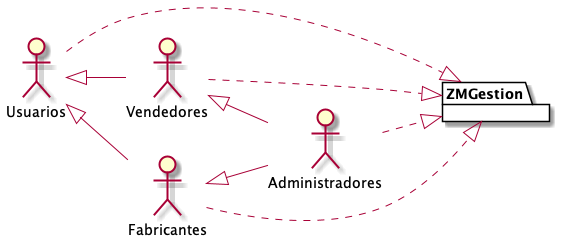
\includegraphics[width=\textwidth,height=0.40\textheight,keepaspectratio]{ModeladoDeCasosDeUso/DiagramaDeCasosDeUso/DiagramaContexto}
		\caption{Diagrama de contexto}
	\label{fig:DiagramaContexto}
	\end{figure}
    \subsection{Diagrama de subsistema}
	\begin{figure}[H]
		\centering
		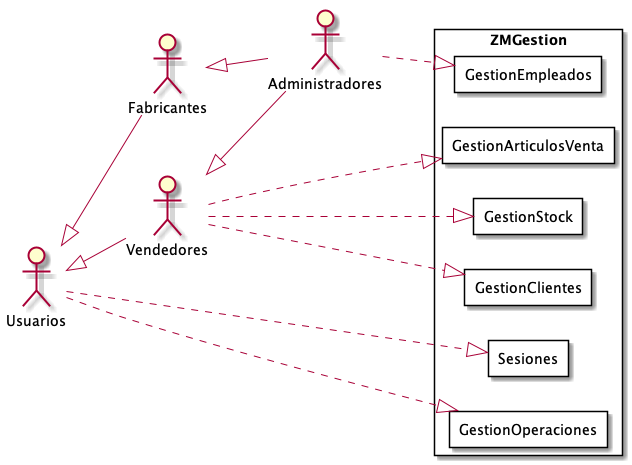
\includegraphics[width=\textwidth,height=0.90\textheight,keepaspectratio]{ModeladoDeCasosDeUso/DiagramaDeCasosDeUso/DiagramaSubsistema}
		\caption{Diagrama de subsistema}
	\label{fig:DiagramaSubsistema}
	\end{figure}
	\subsection{Listado de casos de uso}
	\label{sec:listadoCasoUso}
	\begin{itemize}
		\item Sesiones
		\begin{itemize}
			\itemCaseUse{iniciarSesion}{Iniciar sesión}
			\itemCaseUse{cerrarSesion}{Cerrar sesión}
		\end{itemize}
		\item Gestión empleados
		\begin{itemize}
			\itemCaseUse{crearEmpleado}{Crear empleado}
			\itemCaseUse{buscarAvanzadoEmpleados}{Buscar avanzado empleados}
			\itemCaseUse{darBajaEmpleado}{Dar de baja empleado}
			\itemCaseUse{darAltaEmpleado}{Dar de alta empleado}
			\itemCaseUse{modificarEmpleado}{Modificar empleado}
			\itemCaseUse{borrarEmpleado}{Borrar empleado}
		\end{itemize}
		\item Gestión roles
		\begin{itemize}
			\item Quitar esto cuando se descomente alguna línea de abajo
			%\itemCaseUse{crearRol}{Crear rol}
			%\itemCaseUse{listarRoles}{Listar roles}
			%\itemCaseUse{modificarRol}{Modificar rol}
			%\itemCaseUse{borrarRol}{Borrar rol}
		\end{itemize}
		\item Gestión productos
		\begin{itemize}
			\itemCaseUse{crearProducto}{Crear producto}
			\itemCaseUse{buscarAvanzadoProductos}{Buscar avanzado productos}
			\itemCaseUse{darBajaProducto}{Dar de baja producto}
			\itemCaseUse{darAltaProducto}{Dar de alta producto}
			\itemCaseUse{modificarProducto}{Modificar producto}
			\itemCaseUse{borrarProducto}{Borrar producto}
		\end{itemize}
		\item Gestión telas
		\begin{itemize}
			\itemCaseUse{crearTela}{Crear tela}
			\itemCaseUse{listarTelas}{Listar telas}
			\itemCaseUse{darBajaTela}{Dar de baja tela}
			\itemCaseUse{darAltaTela}{Dar de alta tela}
			\itemCaseUse{modificarTela}{Modificar tela}
			\itemCaseUse{borrarTela}{Borrar tela}
		\end{itemize}
		\item Gestión productos finales
		\begin{itemize}
			\item Quitar esto cuando se descomente alguna línea de abajo
			%\itemCaseUse{crearProductoFinal}{Crear producto final}
			%\itemCaseUse{buscarAvanzadoProductosFinales}{Buscar avanzado productos finales}
			%\itemCaseUse{darBajaProductoFinal}{Dar de baja producto final}
			%\itemCaseUse{darAltaProductoFinal}{Dar de alta producto final}
			%\itemCaseUse{modificarProductoFinal}{Modificar producto final}
			%\itemCaseUse{borrarProductoFinal}{Borrar producto final}
		\end{itemize}
		\item Gestión grupos de producto
		\begin{itemize}
			\item Quitar esto cuando se descomente alguna línea de abajo
			%\itemCaseUse{crearGrupoProducto}{Crear grupo de producto}
			%\itemCaseUse{listarGruposProducto}{Listar grupos de producto}
			%\itemCaseUse{darBajaGrupoProducto}{Dar de baja grupo de producto}
			%\itemCaseUse{darAltaGrupoProducto}{Dar de alta grupo de producto}
			%\itemCaseUse{modificarGrupoProducto}{Modificar grupo de producto}
			%\itemCaseUse{borrarGrupoProducto}{Borrar grupo de producto}
			%\itemCaseUse{listarProductosGrupo}{Listar productos por grupo}
			%\itemCaseUse{modificarPreciosGrupo}{Modificar precios grupo}
		\end{itemize}
		\item Gestión ubicaciones
		\begin{itemize}
			\item Quitar esto cuando se descomente alguna línea de abajo
			%\itemCaseUse{crearUbicacion}{Crear ubicación}
			%\itemCaseUse{listarUbicaciones}{Listar ubicaciones}
			%\itemCaseUse{darBajaUbicacion}{Dar de baja ubicación}
			%\itemCaseUse{darAltaUbicacion}{Dar de alta ubicación}
			%\itemCaseUse{modificarUbicacion}{Modificar ubicación}
			%\itemCaseUse{borrarUbicacion}{Borrar ubicación}
		\end{itemize}
		\item Gestión clientes
		\begin{itemize}
			\item Quitar esto cuando se descomente alguna línea de abajo
			%\itemCaseUse{crearCliente}{Crear cliente}
			%\itemCaseUse{buscarAvanzadoClientes}{Buscar avanzado clientes}
			%\itemCaseUse{darBajaCliente}{Dar de baja cliente}
			%\itemCaseUse{darAltaCliente}{Dar de alta cliente}
			%\itemCaseUse{modificarCliente}{Modificar cliente}
			%\itemCaseUse{borrarCliente}{Borrar cliente}
		\end{itemize}
		\item Gestión presupuestos
		\begin{itemize}
			\item Quitar esto cuando se descomente alguna línea de abajo
			%\itemCaseUse{crearPresupuesto}{Crear presupuesto}
			%\itemCaseUse{buscarAvanzadoPresupuestos}{Buscar avanzado presupuestos}
			%\itemCaseUse{modificarPresupuesto}{Modificar presupuesto}
			%\itemCaseUse{borrarPresupuesto}{Borrar presupuesto}
			%\itemCaseUse{transformarPresupuestoEnVenta}{Transformar presupuesto en venta}
			%\itemCaseUse{generarPresupuestoPDF}{Generar presupuesto en formato PDF}
			%\itemCaseUse{enviarPresupuestoEmail}{Enviar presupuesto por correo electrónico}
			%\itemCaseUse{listarLineasPresupuesto}{Listar líneas de presupuesto}
			
			
		\end{itemize}
		\item Gestión líneas de presupuesto
		\begin{itemize}
			\item Quitar esto cuando se descomente alguna línea de abajo
			%\itemCaseUse{crearLineaPresupuesto}{Crear línea de presupuesto}
			%\itemCaseUse{modificarLineaPresupuesto}{Modificar línea de presupuesto}
			%\itemCaseUse{borrarLineaPresupuesto}{Borrar línea de presupuesto}
		\end{itemize}
		\item Gestión ventas
		\begin{itemize}
			\item Quitar esto cuando se descomente alguna línea de abajo
			%\itemCaseUse{crearVenta}{Crear venta}
			%\itemCaseUse{buscarAvanzadoVentas}{Buscar avanzado ventas}
			%\itemCaseUse{listarLineasVenta}{Listar líneas de venta}
			%\itemCaseUse{modificarVenta}{Modificar venta}
			%\itemCaseUse{borrarVenta}{Borrar venta}
			%\itemCaseUse{generarOrdenProduccionDesdeVenta}{Generar orden de producción a partir de venta}
		\end{itemize}
		\item Gestión líneas de venta
		\begin{itemize}
			\item Quitar esto cuando se descomente alguna línea de abajo
			%\itemCaseUse{crearLineaVenta}{Crear línea de venta}
			%\itemCaseUse{modificarLineaVenta}{Modificar línea de venta}
			%\itemCaseUse{borrarLineaVenta}{Borrar línea de venta}
		\end{itemize}
		\item Gestión facturas
		\begin{itemize}
			\item Quitar esto cuando se descomente alguna línea de abajo
			%\itemCaseUse{crearFactura}{Crear factura}
			%\itemCaseUse{buscarAvanzadoFacturas}{Buscar avanzado facturas}
			%\itemCaseUse{darBajaFactura}{Dar de baja factura}
			%\itemCaseUse{darAltaFactura}{Dar de alta factura}
			%\itemCaseUse{modificarFactura}{Modificar factura}
			%\itemCaseUse{borrarFactura}{Borrar factura}
		\end{itemize}
		\item Gestión recibos
		\begin{itemize}
			\item Quitar esto cuando se descomente alguna línea de abajo
			%\itemCaseUse{crearRecibo}{Crear recibo}
			%\itemCaseUse{buscarAvanzadoRecibos}{Buscar avanzado recibos}
			%\itemCaseUse{darBajaRecibo}{Dar de baja recibo}
			%\itemCaseUse{darAltaRecibo}{Dar de alta recibo}
			%\itemCaseUse{modificarRecibo}{Modificar recibo}
			%\itemCaseUse{borrarRecibo}{Borrar recibo}
		\end{itemize}
		\item Gestión notas de crédito
		\begin{itemize}
			\item Quitar esto cuando se descomente alguna línea de abajo
			%\itemCaseUse{crearNotaCredito}{Crear nota de crédito}
			%\itemCaseUse{buscarAvanzadoNotasCredito}{Buscar avanzado notas de crédito}
			%\itemCaseUse{darBajaNotaCredito}{Dar de baja nota de crédito}
			%\itemCaseUse{darAltaNotaCredito}{Dar de alta nota de crédito}
			%\itemCaseUse{modificarNotaCredito}{Modificar nota de crédito}
			%\itemCaseUse{borrarNotaCredito}{Borrar nota de crédito}
		\end{itemize}
		\item Gestión remitos
		\begin{itemize}
			\item Quitar esto cuando se descomente alguna línea de abajo
			%\itemCaseUse{crearRemito}{Crear remito}
			%\itemCaseUse{buscarAvanzadoRemitos}{Buscar avanzado remitos}
			%\itemCaseUse{darBajaRemito}{Dar de baja remito}
			%\itemCaseUse{darAltaRemito}{Dar de alta remito}
			%\itemCaseUse{borrarRemito}{Borrar remito}
		\end{itemize}
		\item Gestión órdenes de reposición
		\begin{itemize}
			\item Quitar esto cuando se descomente alguna línea de abajo
			%\itemCaseUse{crearOrdenReposicion}{Crear orden de reposición}
			%\itemCaseUse{buscarAvanzadoOrdenesReposicion}{Buscar avanzado órdenes de reposición}
			%\itemCaseUse{darBajaOrdenReposicion}{Dar de baja orden de reposición}
			%\itemCaseUse{darAltaOrdenReposicion}{Dar de alta orden de reposición}
			%\itemCaseUse{borrarOrdenReposicion}{Borrar orden de reposición}
		\end{itemize}
		\item Gestión órdenes de producción
		\begin{itemize}
			\item Quitar esto cuando se descomente alguna línea de abajo
			%\itemCaseUse{crearOrdenProduccion}{Crear orden de producción}
			%\itemCaseUse{buscarAvanzadoOrdenesProduccion}{Buscar avanzado órdenes de producción}
			%\itemCaseUse{modificarOrdenProduccion}{Modificar orden de producción}
			%\itemCaseUse{listarLineasOrdenProduccion}Listar lineas de orden de producción}
			%\itemCaseUse{borrarOrdenProduccion}{Borrar orden de producción}
			%\itemCaseUse{finalizarOrdenProduccion}{Finalizar orden de producción}
			%\itemCaseUse{verificarOrdenProduccion}{Verificar orden de producción}
			%\itemCaseUse{producirOrdenProduccion}{Producir orden de producción}
			%\itemCaseUse{cancelarOrdenProduccion}{Cancelar orden de producción}
			%\itemCaseUse{listarObservacionesLineaOrdenProduccion}{Listar observaciones de línea de orden de producción}
		\end{itemize}
		\item Gestión líneas de órdenes de producción
		\begin{itemize}
			\item Quitar esto cuando se descomente alguna línea de abajo
			%\itemCaseUse{crearLineaOrdenProduccion}{Crear línea de orden de producción}
			%\itemCaseUse{modificarLineaOrdenProduccion}{Modificar línea de orden de producción}
			%\itemCaseUse{borrarLineaOrdenProduccion}{Borrar línea de orden de producción}
			%\itemCaseUse{finalizarLineaOrdenProduccion}{Finalizar línea de orden de producción}
			%\itemCaseUse{verificarLineaOrdenProduccion}{Verificar línea de orden de producción}
			%\itemCaseUse{asignarFabricanteLineaOrdenProduccion}{Asignar fabricante a línea de orden de producción}
			%\itemCaseUse{producirLineaOrdenProduccion}{Producir línea de orden de producción}
			%\itemCaseUse{cancelarLineaOrdenProduccion}{Cancelar línea de orden de producción}		
			
		\end{itemize}
		\item Gestión observaciones
		\begin{itemize}
			\item Quitar esto cuando se descomente alguna línea de abajo
			%\itemCaseUse{crearObservacion}{Crear observación}
			%\itemCaseUse{borrarObservacion}{Borrar observación}
		\end{itemize}
	\end{itemize}	
	\subsection{Diagrama de casos de uso}
	\begin{figure}[H]
		\centering
		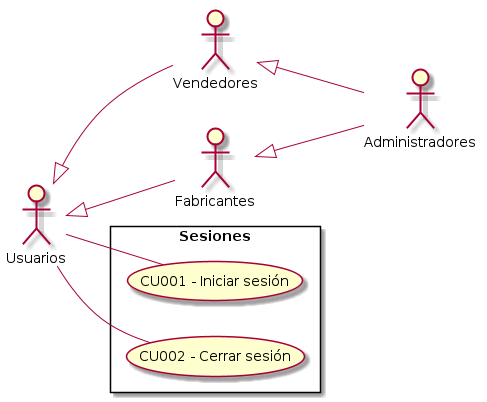
\includegraphics[width=\textwidth,height=0.30\textheight,keepaspectratio]{ModeladoDeCasosDeUso/DiagramaDeCasosDeUso/Sesiones}
		\caption{Diagrama de casos de uso para sesiones}
	\label{fig:Sesiones}
	\end{figure}
	\begin{figure}[H]
		\centering
		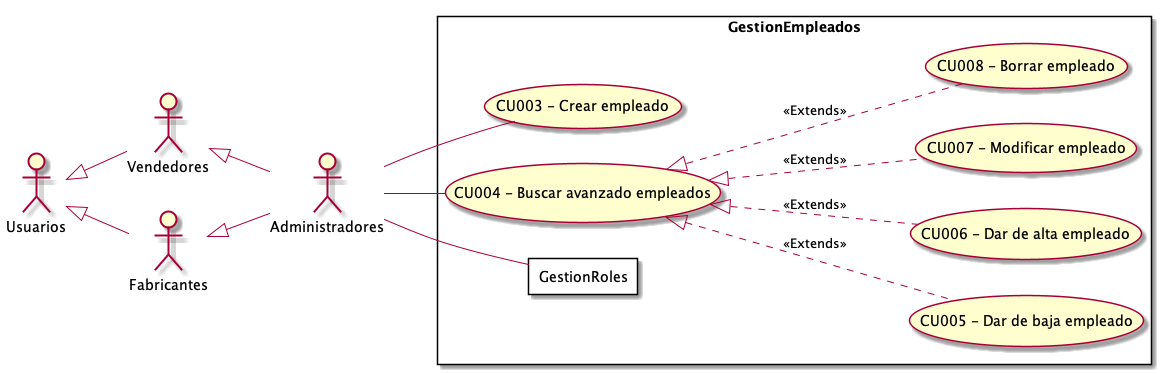
\includegraphics[width=\textwidth,height=0.40\textheight,keepaspectratio]{ModeladoDeCasosDeUso/DiagramaDeCasosDeUso/GestionEmpleados}
		\caption{Diagrama de casos de uso para la gestión de empleados}
	\label{fig:GestionEmpleados}
	\end{figure}
	\begin{figure}[H]
		\centering
		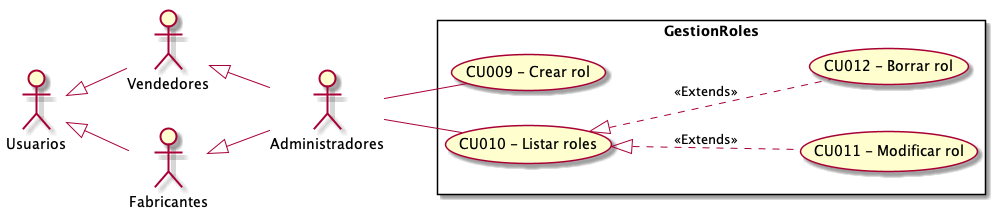
\includegraphics[width=\textwidth,height=0.90\textheight,keepaspectratio]{ModeladoDeCasosDeUso/DiagramaDeCasosDeUso/GestionRoles}
		\caption{Diagrama de casos de uso para la gestión de roles}
	\label{fig:GestionRoles}
    \end{figure}
    \begin{figure}[H]
		\centering
		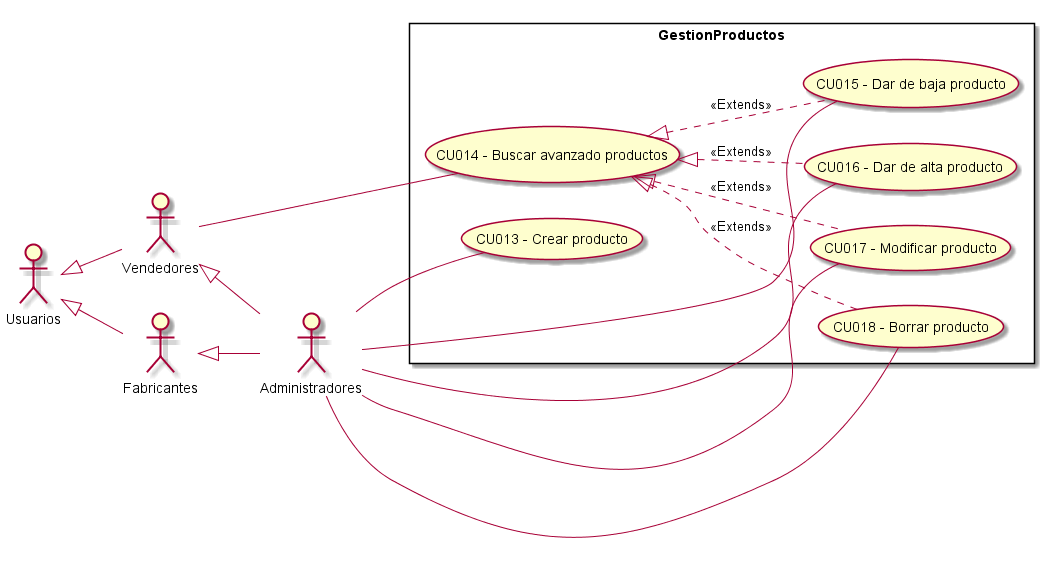
\includegraphics[width=\textwidth,height=0.90\textheight,keepaspectratio]{ModeladoDeCasosDeUso/DiagramaDeCasosDeUso/GestionProductos}
		\caption{Diagrama de casos de uso para la gestión de productos}
	\label{fig:GestionProductos}
    \end{figure}
    \begin{figure}[H]
		\centering
		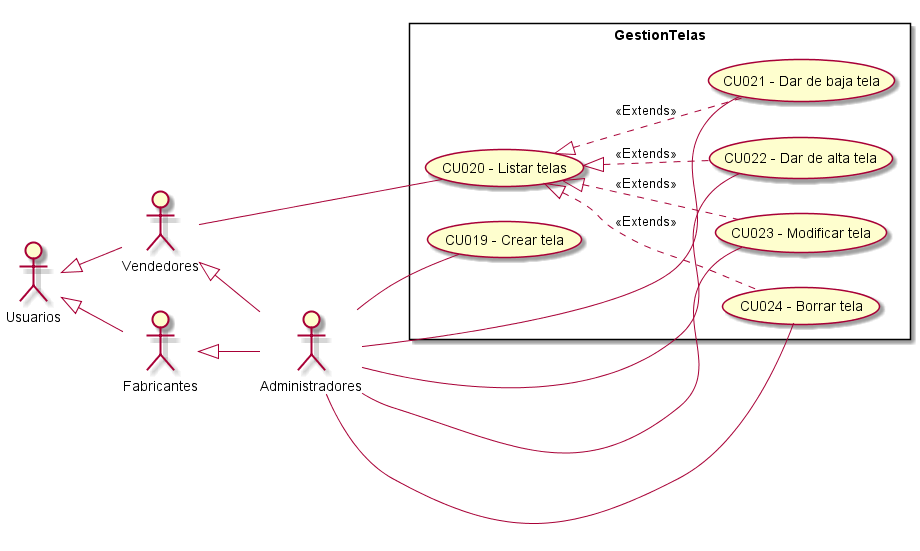
\includegraphics[width=\textwidth,height=0.90\textheight,keepaspectratio]{ModeladoDeCasosDeUso/DiagramaDeCasosDeUso/GestionTelas}
		\caption{Diagrama de casos de uso para la gestión de telas}
	\label{fig:GestionTelas}
    \end{figure}
    \begin{figure}[H]
		\centering
		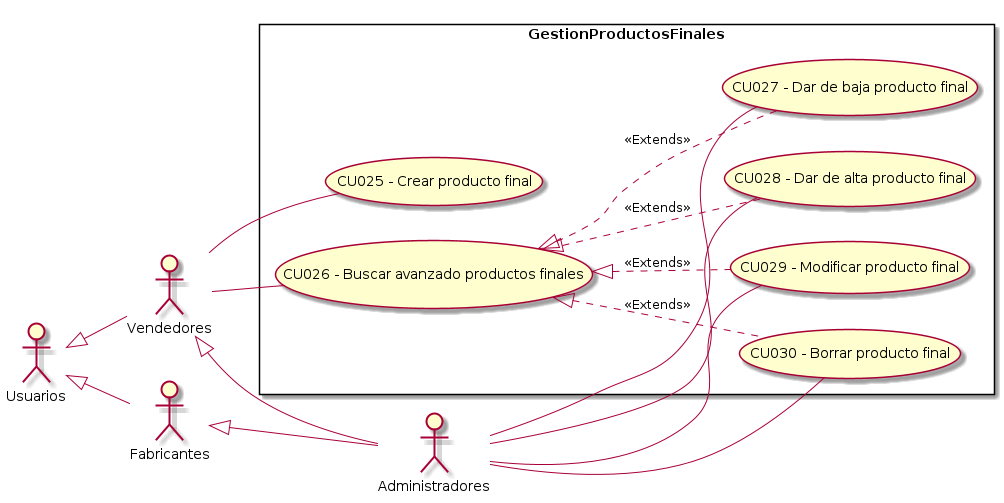
\includegraphics[width=\textwidth,height=0.90\textheight,keepaspectratio]{ModeladoDeCasosDeUso/DiagramaDeCasosDeUso/GestionProductosFinales}
		\caption{Diagrama de casos de uso para la gestión de productos finales}
	\label{fig:GestionProductosFinales}
    \end{figure}
    \begin{figure}[H]
		\centering
		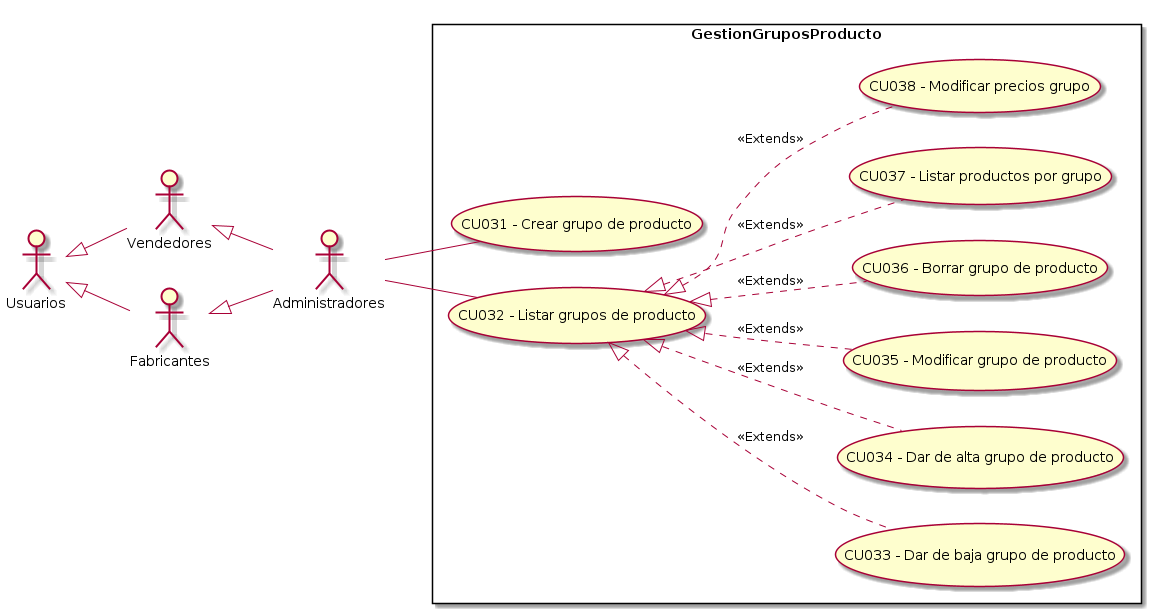
\includegraphics[width=\textwidth,height=0.90\textheight,keepaspectratio]{ModeladoDeCasosDeUso/DiagramaDeCasosDeUso/GestionGruposProducto}
		\caption{Diagrama de casos de uso para la gestión de grupos de producto}
	\label{fig:GestionGruposProducto}
    \end{figure}
    \begin{figure}[H]
		\centering
		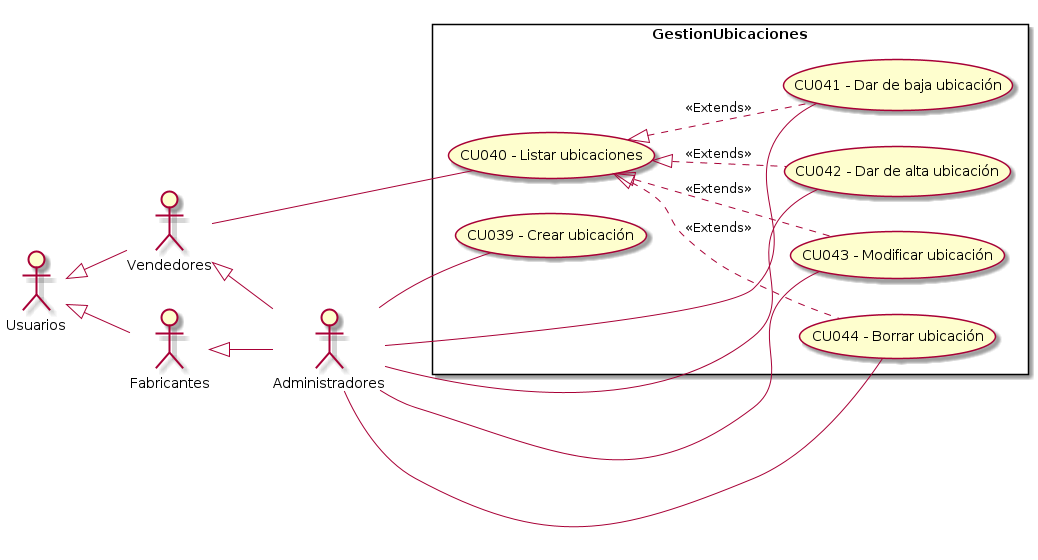
\includegraphics[width=\textwidth,height=0.90\textheight,keepaspectratio]{ModeladoDeCasosDeUso/DiagramaDeCasosDeUso/GestionUbicaciones}
		\caption{Diagrama de casos de uso para la gestión de ubicaciones}
	\label{fig:GestionUbicaciones}
    \end{figure}
    \begin{figure}[H]
		\centering
		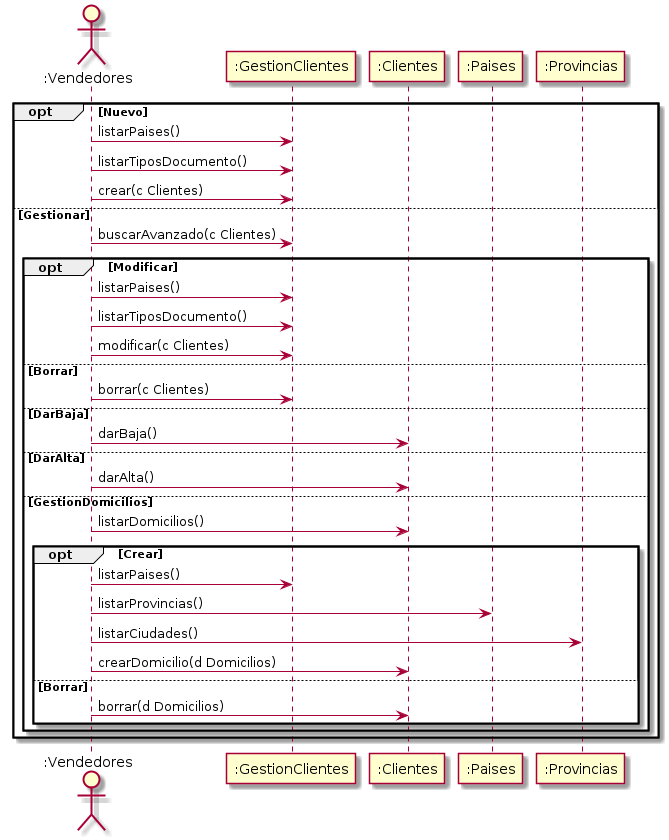
\includegraphics[width=\textwidth,height=0.90\textheight,keepaspectratio]{ModeladoDeCasosDeUso/DiagramaDeCasosDeUso/GestionClientes}
		\caption{Diagrama de casos de uso para la gestión de clientes}
	\label{fig:GestionClientes}
    \end{figure}
    \begin{figure}[H]
		\centering
		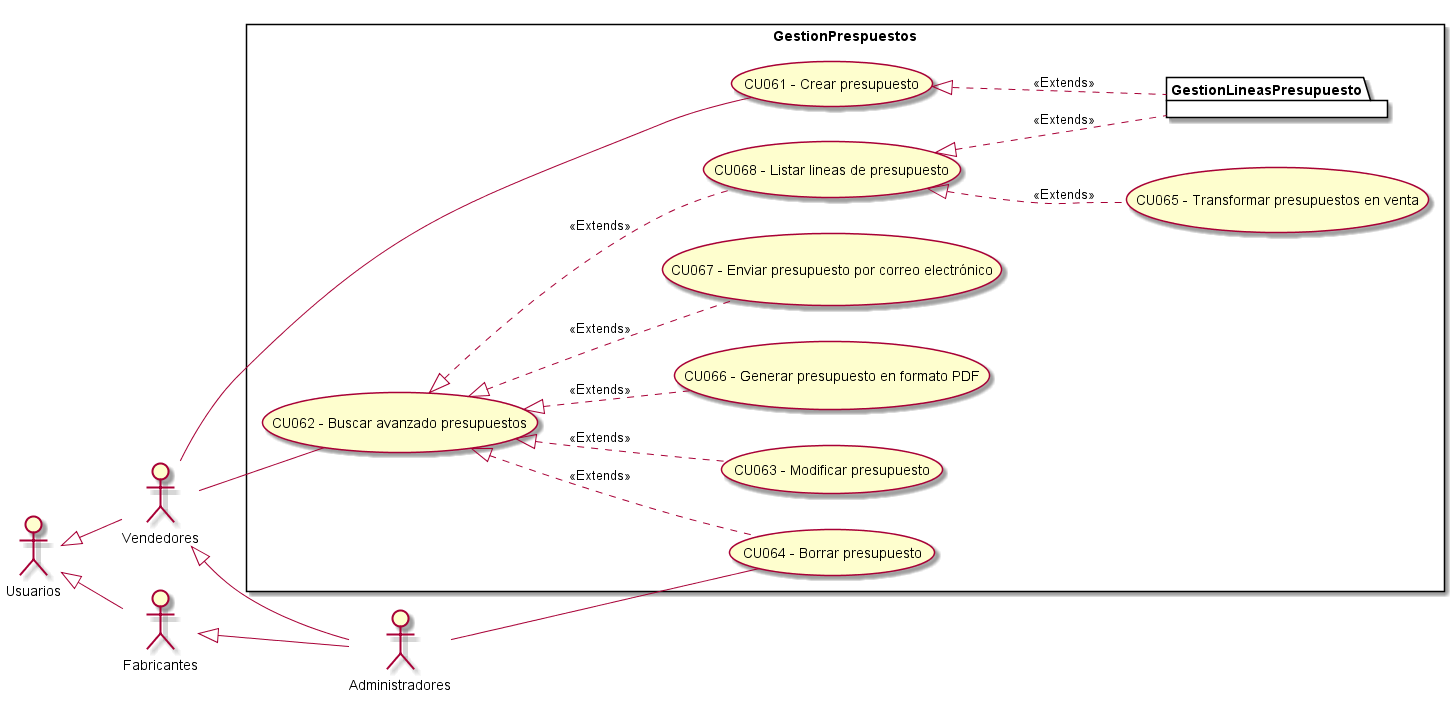
\includegraphics[width=\textwidth,height=0.90\textheight,keepaspectratio]{ModeladoDeCasosDeUso/DiagramaDeCasosDeUso/GestionPresupuestos}
		\caption{Diagrama de casos de uso para la gestión de presupuestos}
	\label{fig:GestionPresupuestos}
    \end{figure}
    \begin{figure}[H]
		\centering
		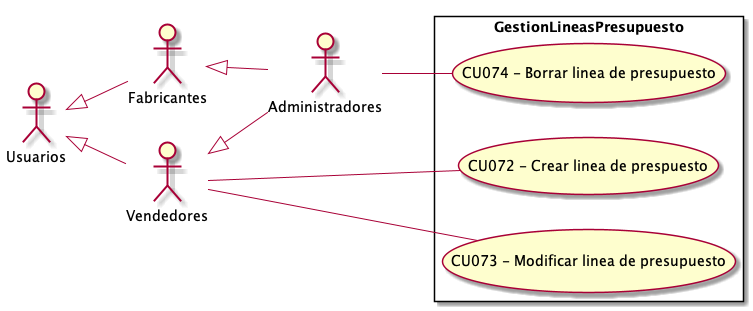
\includegraphics[width=\textwidth,height=0.90\textheight,keepaspectratio]{ModeladoDeCasosDeUso/DiagramaDeCasosDeUso/GestionLineasPresupuesto}
		\caption{Diagrama de casos de uso para la gestión de líneas de presupuesto}
	\label{fig:GestionLineasPresupuesto}
    \end{figure}
    \begin{figure}[H]
		\centering
		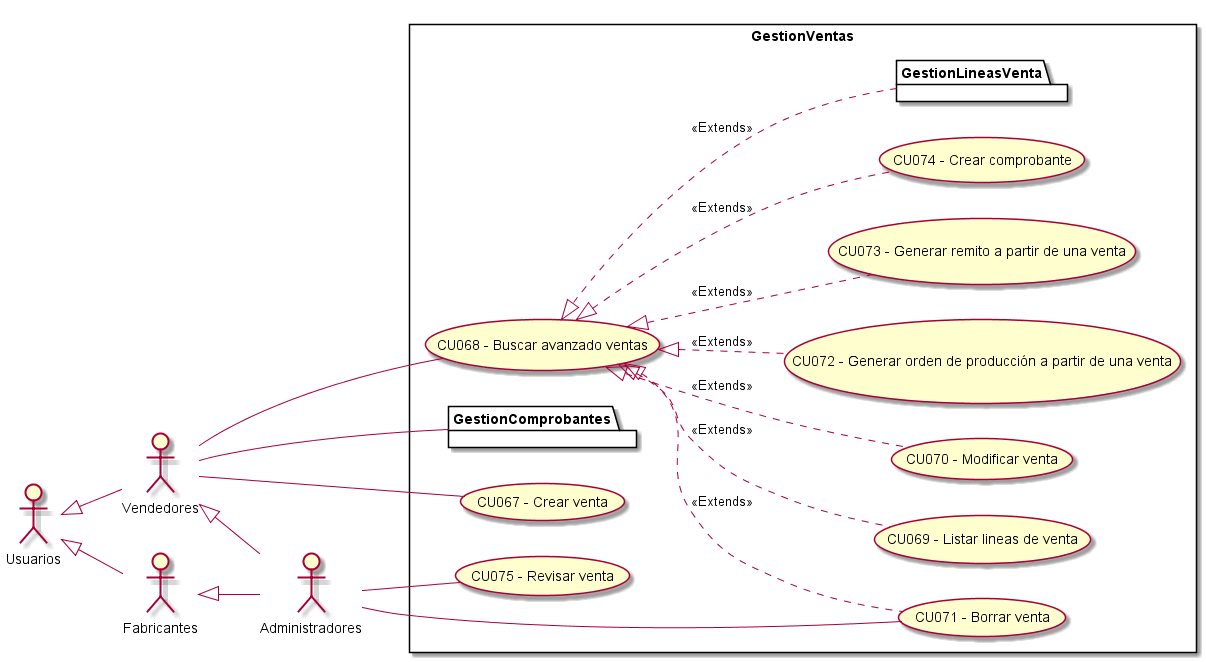
\includegraphics[width=\textwidth,height=0.90\textheight,keepaspectratio]{ModeladoDeCasosDeUso/DiagramaDeCasosDeUso/GestionVentas}
		\caption{Diagrama de casos de uso para la gestión de ventas}
	\label{fig:GestionVentas}
    \end{figure}
    \begin{figure}[H]
		\centering
		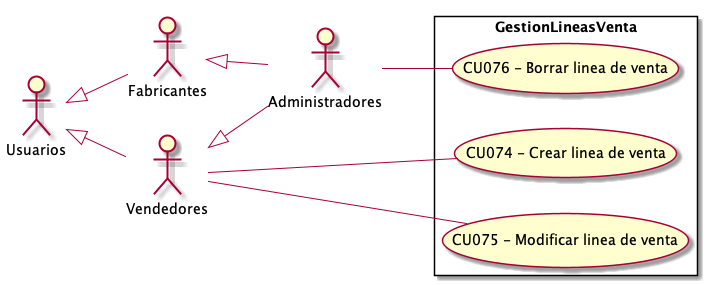
\includegraphics[width=\textwidth,height=0.90\textheight,keepaspectratio]{ModeladoDeCasosDeUso/DiagramaDeCasosDeUso/GestionLineasVenta}
		\caption{Diagrama de casos de uso para la gestión de líneas de venta}
	\label{fig:GestionLineasVenta}
    \end{figure}
    \begin{figure}[H]
		\centering
		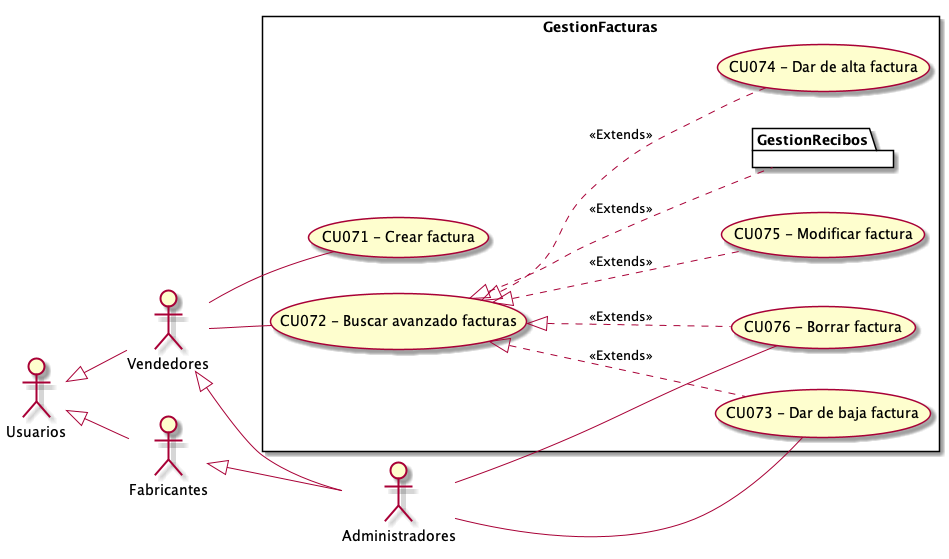
\includegraphics[width=\textwidth,height=0.90\textheight,keepaspectratio]{ModeladoDeCasosDeUso/DiagramaDeCasosDeUso/GestionFacturas}
		\caption{Diagrama de casos de uso para la gestión de facturas}
	\label{fig:GestionFacturas}
    \end{figure}
    \begin{figure}[H]
		\centering
		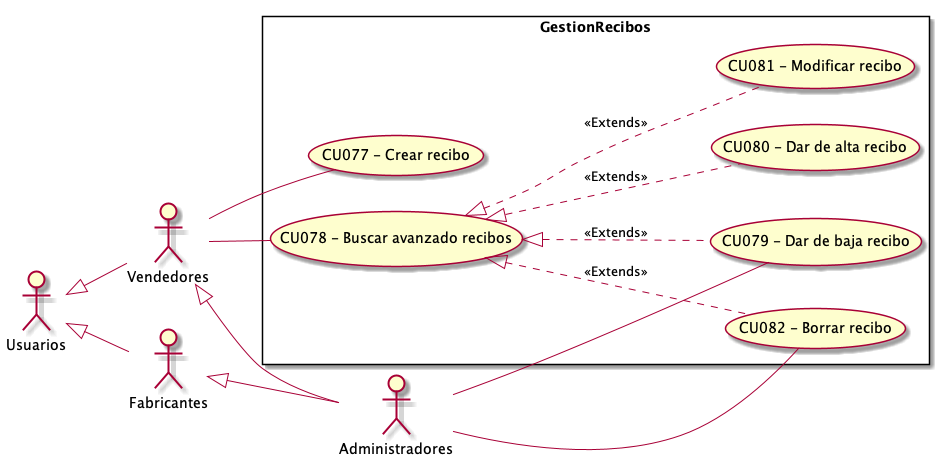
\includegraphics[width=\textwidth,height=0.90\textheight,keepaspectratio]{ModeladoDeCasosDeUso/DiagramaDeCasosDeUso/GestionRecibos}
		\caption{Diagrama de casos de uso para la gestión de recibos}
	\label{fig:GestionRecibos}
    \end{figure}
    \begin{figure}[H]
		\centering
		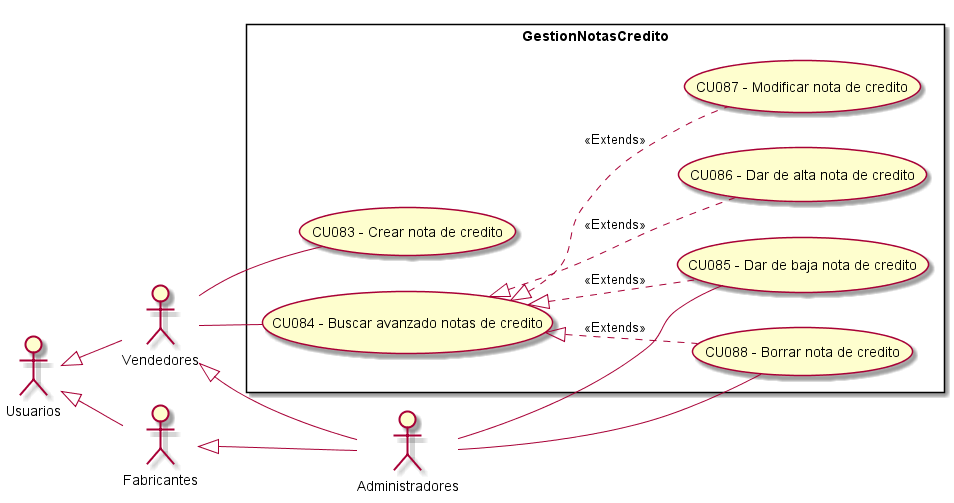
\includegraphics[width=\textwidth,height=0.90\textheight,keepaspectratio]{ModeladoDeCasosDeUso/DiagramaDeCasosDeUso/GestionNotasCredito}
		\caption{Diagrama de casos de uso para la gestión de notas de crédito}
	\label{fig:GestionNotasCredito}
    \end{figure}
    \begin{figure}[H]
		\centering
		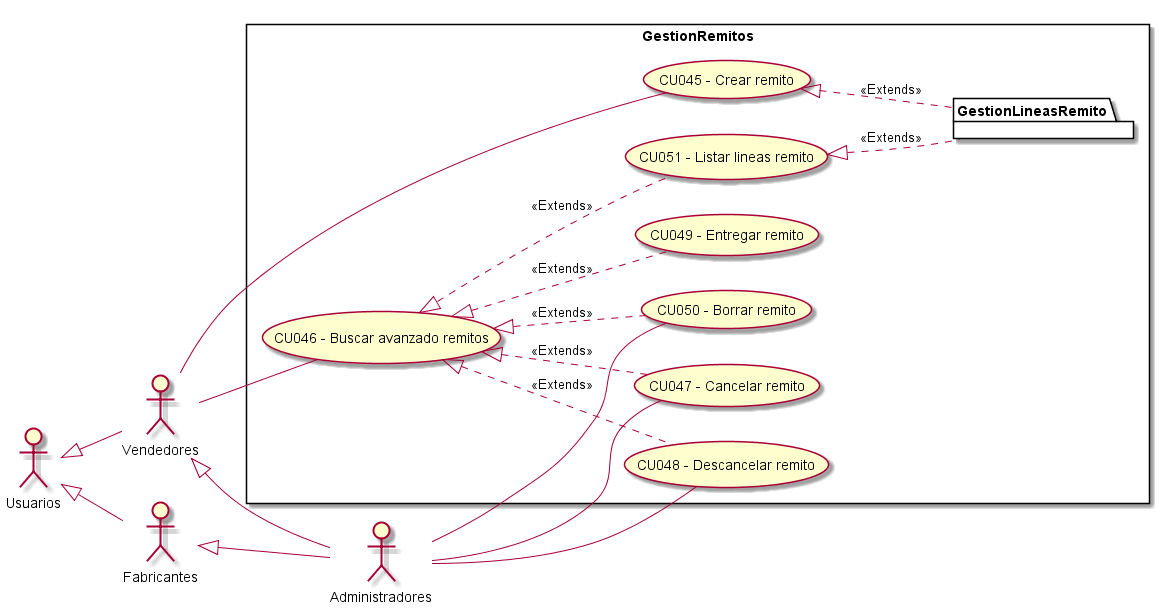
\includegraphics[width=\textwidth,height=0.90\textheight,keepaspectratio]{ModeladoDeCasosDeUso/DiagramaDeCasosDeUso/GestionRemitos}
		\caption{Diagrama de casos de uso para la gestión de remitos}
	\label{fig:GestionRemitos}
    \end{figure}
    \begin{figure}[H]
		\centering
		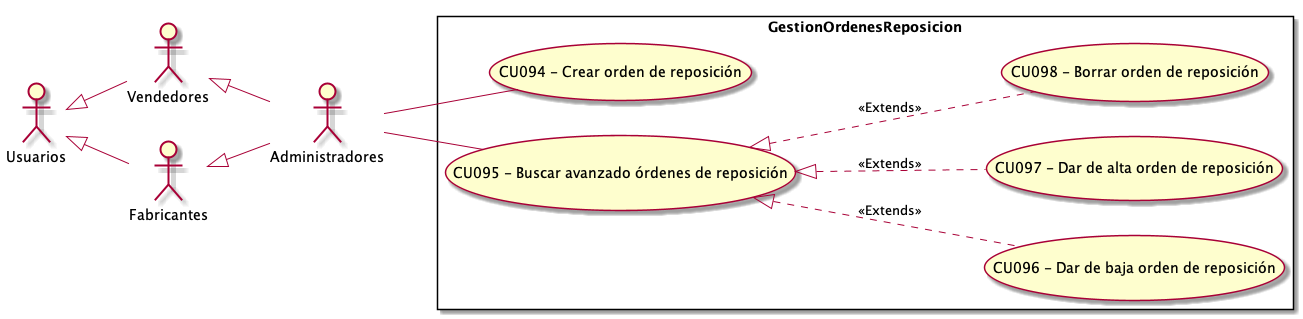
\includegraphics[width=\textwidth,height=0.90\textheight,keepaspectratio]{ModeladoDeCasosDeUso/DiagramaDeCasosDeUso/GestionOrdenesReposicion}
		\caption{Diagrama de casos de uso para la gestión de órdenes de reposición}
	\label{fig:GestionOrdenesReposicion}
    \end{figure}
    \begin{figure}[H]
		\centering
		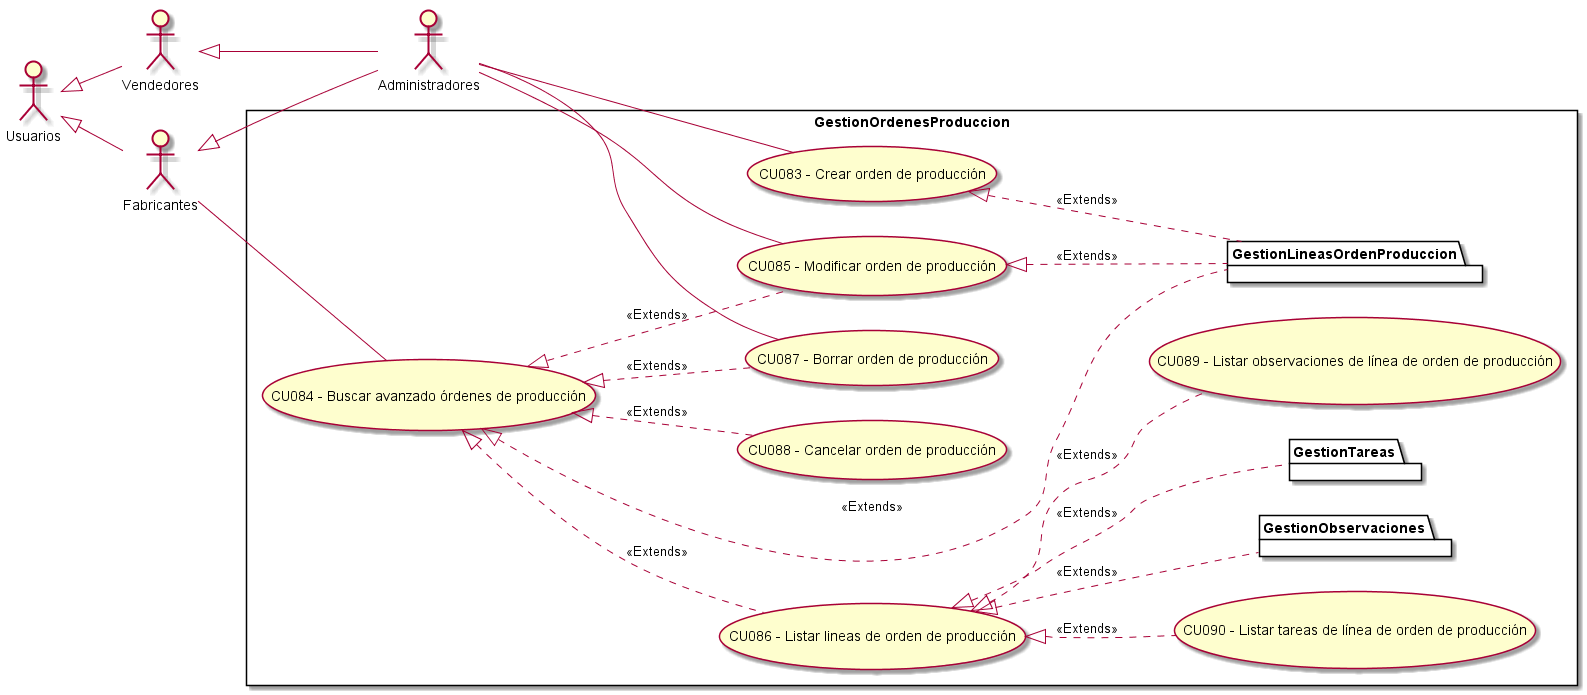
\includegraphics[width=\textwidth,height=0.90\textheight,keepaspectratio]{ModeladoDeCasosDeUso/DiagramaDeCasosDeUso/GestionOrdenesProduccion}
		\caption{Diagrama de casos de uso para la gestión de órdenes de producción}
	\label{fig:GestionOrdenesProduccion}
    \end{figure}
    \begin{figure}[H]
		\centering
		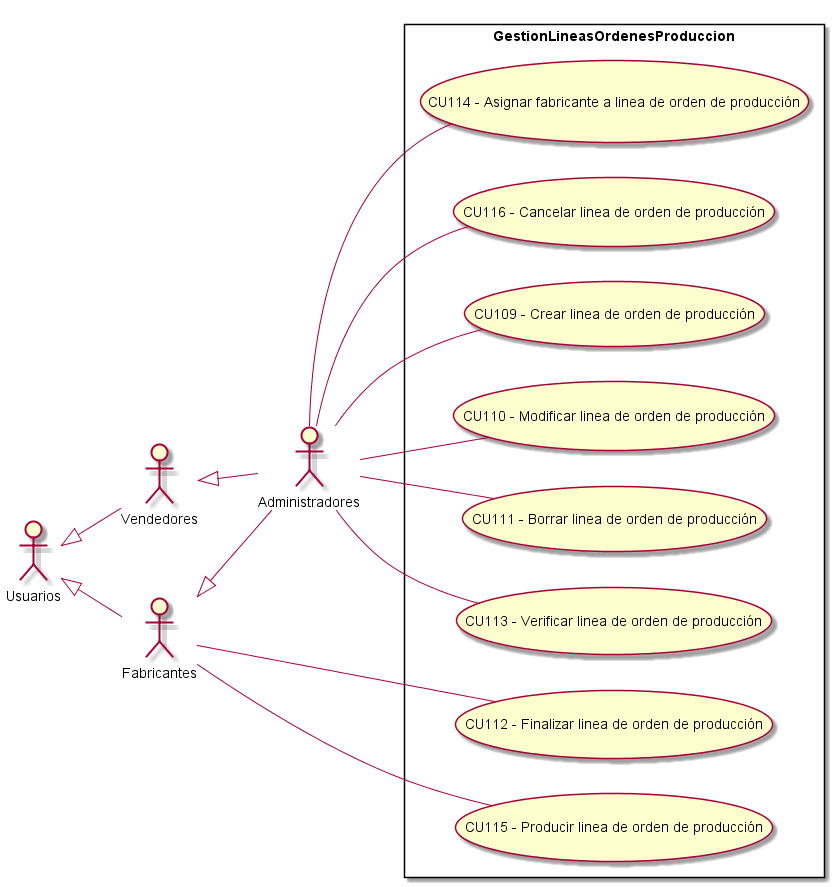
\includegraphics[width=\textwidth,height=0.90\textheight,keepaspectratio]{ModeladoDeCasosDeUso/DiagramaDeCasosDeUso/GestionLineasOrdenesProduccion}
		\caption{Diagrama de casos de uso para la gestión de líneas de órdenes de producción}
	\label{fig:GestionLineasOrdenesProduccion}
    \end{figure}
    \begin{figure}[H]
		\centering
		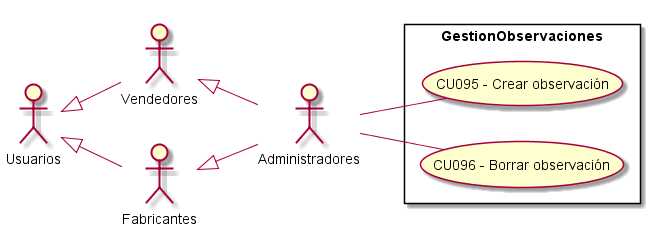
\includegraphics[width=\textwidth,height=0.90\textheight,keepaspectratio]{ModeladoDeCasosDeUso/DiagramaDeCasosDeUso/GestionObservaciones}
		\caption{Diagrama de casos de uso para la gestión de observaciones}
	\label{fig:GestionObservaciones}
	\end{figure}
	\clearpage %salto de pagina
	\subsection{Descripción textual de los casos de uso}
		\begin{enumerate}
			%Sesiones
			\renewcommand{\caseUseShortName}{iniciarSesion}
\renewcommand{\caseUseCreated}{16/01/2020}
\renewcommand{\caseUseModified}{16/01/2020}
\renewcommand{\caseUseName}{\CUiniciarSesion - Iniciar sesión}
\renewcommand{\caseUseSummary}{Este caso de uso permite a un usuario iniciar sesión en el sistema.}
\renewcommand{\caseUsePeople}{Usuarios: quiere ingresar al sistema.}
\renewcommand{\caseUsePreconditions}{
	\caseUseRow{El usuario se encuentra creado y activo en ZMGestion.}
}
\renewcommand{\caseUsePostconditions}{
	\caseUseRow{Se valida al usuario y se le muestra al usuario las opciones personales disponibles.}
}
\renewcommand{\caseUseScene}{
	\addCaseUseStep{El usuario ingresa la dirección de la aplicación en un dispositivo conectado a Internet.}
	\addCaseUseStep{ZMGestion muestra un formulario para que el usuario ingrese su nombre de usuario y contraseña.}
	\addCaseUseStep{El usuario introduce su nombre de usuario y contraseña.}
	\addCaseUseStep{ZMGestion trae los permisos del usuario y le muestra sus opciones.}
	
}
\renewcommand{\alternativeCaseUse}{
	\newAlternative{A1: El nombre de usuario no existe en ZMGestion.}{3}
	\caseUseRow{La secuencia A1 comienza luego del punto 3 del escenario principal.}
	\alternativeRow{ZMGestion muestra un mensaje de error.}
	\caseUseRow{El escenario vuelve al punto 2.}
	\caseUseRow{}
	
	\newAlternative{A2: El usuario no se encuentra activo.}{3}
	\caseUseRow{La secuencia A2 comienza luego del punto 3 del escenario principal.}
	\alternativeRow{ZMGestion informa al usuario que el mismo no se encuentra activo y que debe comuicarse con un administrador.}
	\caseUseRow{El escenario vuelve al punto 2.}
	\caseUseRow{}

	\newAlternative{A3: La contraseña ingresada es incorrecta y el número de intentos no supero el límite permitido.}{3}
	\caseUseRow{La secuencia A3 comienza luego del punto 3 del escenario principal.}
	\alternativeRow{ZMGestion informa al usuario que la contraseña ingresada es incorrecta.}
	\caseUseRow{El escenario vuelve al punto 2.}
	\caseUseRow{}

	\newAlternative{A4: La contraseña ingresada es incorrecta y el número de intentos supero el límite permitido.}{3}
	\caseUseRow{La secuencia A4 comienza luego del punto 3 del escenario principal.}
	\alternativeRow{ZMGestion informa al usuario que la contraseña es incorrecta, que el usuario ha sido ha sido dado de baja y que debe comunicarse con un administrador.}
	\caseUseRow{El escenario vuelve al punto 2.}
	\caseUseRow{}	
}

\item Caso de uso \caseUseName

%DESCRIPCION TEXTUAL
\renewcommand*{\arraystretch}{1.3}
\begin{longtable}[c]{|>{\raggedright}p{0.3\textwidth} | >{\raggedright}p{0.2\textwidth} | p{0.5\textwidth} |}
\caption{\hyperref[sec:listadoCasoUso]{\caseUseName}}
\label{tabla:\caseUseShortName}\\
\hline
\rowcolor{tableCaseUseBackground}

\multicolumn{3}{|l|}{\textcolor{tableCaseUseFontColor}{Descripción textual del caso de uso: \caseUseName}} \\ \hline

Fecha de Creación: & \multicolumn{2}{L{\secondColumnWidth}|}{\caseUseCreated}\\ \hline

Fecha de Modificación: & \multicolumn{2}{L{\secondColumnWidth}|}{\caseUseModified} \\ \hline

Versión: & \multicolumn{2}{L{\secondColumnWidth}|}{1} \\ \hline

Resumen: & \multicolumn{2}{L{\secondColumnWidth}|}{\caseUseSummary} \\ \hline

Personas involucradas y metas: & \multicolumn{2}{L{\secondColumnWidth}|}{\caseUsePeople} \\ \hline

Precondiciones: \caseUsePreconditions \hline

Postcondiciones: \caseUsePostconditions \hline

Escenario principal: \caseUseScene \hline

Flujos alternativos: \alternativeCaseUse \hline

Requisitos de interfaz de usuario: \caseUseRequirementsGUI \hline
\multirow{3}{*}{Requisitos funcionales:}  & Tiempo de respuesta: & \caseUseResponseTime \\ \cline{2-3} 
& Concurrencia: & \caseUseConcurrence \\ \cline{2-3} 
& Disponibilidad: & \caseUseAvailability \\ \hline
\end{longtable}

\setcounter{rownumbers}{0}

\renewcommand{\alternativeCaseUse}{
	\caseUseRow{No existen flujos alternativos.}
}

%DIAGRAMA DE ACTIVIDAD
%\lineabreak[0]
\activityDiagram{\caseUseShortName}{Diagrama de actividad - \caseUseName}

			\renewcommand{\caseUseShortName}{cerrarSesion}
\renewcommand{\caseUseCreated}{16/01/2020}
\renewcommand{\caseUseModified}{16/01/2020}
\renewcommand{\caseUseName}{CU02 - Cerrar sesión}
\renewcommand{\caseUseSummary}{Este caso de uso permite a un usuario cerrar sesión en el sistema.}
\renewcommand{\caseUsePeople}{Usuarios: quiere salir del sistema.}
\renewcommand{\caseUsePreconditions}{
	\caseUseRow{Tener una sesión iniciada en el sistema.}
}
\renewcommand{\caseUsePostconditions}{
	\caseUseRow{Se borra el token de sesión almacenado en el dispositivo del usuario.}
}
\renewcommand{\caseUseScene}{
	\addCaseUseStep{El usuario accede a la pantalla destinada para cerrar sesión.}
	\addCaseUseStep{ZMGestion cierra la sesión del usuario y muestra un mensaje informando el éxito de la operación.}
}
\renewcommand{\alternativeCaseUse}{
	\caseUseRow{Ninguno.}
	\caseUseRow{}
}

%\item Caso de uso \caseUseName

%DESCRIPCION TEXTUAL
\renewcommand*{\arraystretch}{1.3}
\begin{longtable}[c]{|>{\raggedright}p{0.3\textwidth} | >{\raggedright}p{0.2\textwidth} | p{0.5\textwidth} |}
\caption{\hyperref[sec:listadoCasoUso]{\caseUseName}}
\label{tabla:\caseUseShortName}\\
\hline
\rowcolor{tableCaseUseBackground}

\multicolumn{3}{|l|}{\textcolor{tableCaseUseFontColor}{Descripción textual del caso de uso: \caseUseName}} \\ \hline

Fecha de Creación: & \multicolumn{2}{L{\secondColumnWidth}|}{\caseUseCreated}\\ \hline

Fecha de Modificación: & \multicolumn{2}{L{\secondColumnWidth}|}{\caseUseModified} \\ \hline

Versión: & \multicolumn{2}{L{\secondColumnWidth}|}{1} \\ \hline

Resumen: & \multicolumn{2}{L{\secondColumnWidth}|}{\caseUseSummary} \\ \hline

Personas involucradas y metas: & \multicolumn{2}{L{\secondColumnWidth}|}{\caseUsePeople} \\ \hline

Precondiciones: \caseUsePreconditions \hline

Postcondiciones: \caseUsePostconditions \hline

Escenario principal: \caseUseScene \hline

Flujos alternativos: \alternativeCaseUse \hline

Requisitos de interfaz de usuario: \caseUseRequirementsGUI \hline
\multirow{3}{*}{Requisitos funcionales:}  & Tiempo de respuesta: & \caseUseResponseTime \\ \cline{2-3} 
& Concurrencia: & \caseUseConcurrence \\ \cline{2-3} 
& Disponibilidad: & \caseUseAvailability \\ \hline
\end{longtable}

\setcounter{rownumbers}{0}

\renewcommand{\alternativeCaseUse}{
	\caseUseRow{No existen flujos alternativos.}
}

%DIAGRAMA DE ACTIVIDAD
%\lineabreak[0]
%\activityDiagram{\caseUseShortName}{Diagrama de actividad - \caseUseName}


			%GestionEmpleados
			
\renewcommand{\caseUseShortName}{crearEmpleado} %cammelCase name

\renewcommand{\caseUseCreated}{27/01/2020} %Fecha creación
\renewcommand{\caseUseModified}{27/01/2020} %Fecha modificación
\renewcommand{\caseUseName}{CU03 - Crear empleado} %{\CUcammelCase - Title}

\renewcommand{\caseUseSummary}{Este caso de uso permite a un administrador de ZMGestion crear empleados y asignarle un rol en el sistema.} %Resumen
\renewcommand{\caseUsePeople}{Administradores: quiere crear un empleado.} %Actor: Meta
\renewcommand{\caseUsePreconditions}{
	\caseUseRow{Haber iniciado sesión en el sistema y tener el permiso necesario para realizar esta función.} %Precondiciones
}
\renewcommand{\caseUsePostconditions}{
	\caseUseRow{Ninguna.} %Postcondiciones
}
\renewcommand{\caseUseScene}{ %Escenario principal
    \addCaseUseStep{El administrador accede a la pantalla para crear empleados}
    \addCaseUseStep{ZMGestion muestra un formulario para que el usuario ingrese: Nombres, apellidos, correo electrónico, número de teléfono, nombre de usuario, contraseña, fecha de inicio de actividad laboral, cantidad de hijos, estado civil, tipo de documento, documento, teléfono, fecha de nacimiento, rol del empleado que desea agregar y su ubicación en la cual desempeñará su tarea. Indicando que son requeridos todos los campos.}
    \addCaseUseStep{El administrador completa los campos del formulario.}
    \addCaseUseStep{ZMGestion crea el empleado con los campos ingresados por el usuario y muestra un mensaje indicando el éxito de la operación.}
}
\renewcommand{\alternativeCaseUse}{ %Flujos alternativos
	\newAlternative{A1: El nombre de usuario ingresado ya existe.}{3} %Flujo alternativo A1.
	\caseUseRow{La secuencia A1 comienza luego del punto 3 del escenario principal.} %¡Indicar número paso!
    \alternativeRow{ZMGestion muestra un mensaje de error informando que el nombre de usuario ingresado ya está en uso.}
    \caseUseRow{El escenario vuelve al punto 2.}
    \caseUseRow{}
    \newAlternative{A2: El correo electrónico ingresado ya existe.}{3} %Flujo alternativo A2.
	\caseUseRow{La secuencia A2 comienza luego del punto 3 del escenario principal.} %¡Indicar número paso!
    \alternativeRow{ZMGestion muestra un mensaje de error informando que el correo electrónico ingresado ya está en uso.}
    \caseUseRow{El escenario vuelve al punto 2.}
    \caseUseRow{}
    \newAlternative{A3: El documento y tipo de documento ingresado ya existe.}{3} %Flujo alternativo A3.
	\caseUseRow{La secuencia A3 comienza luego del punto 3 del escenario principal.} %¡Indicar número paso!
    \alternativeRow{ZMGestion muestra un mensaje de error informando que el documento y tipo de documento ya existe.}
    \caseUseRow{El escenario vuelve al punto 2.}
    \caseUseRow{}
    \newAlternative{A4: El usuario ha dejado un campo requerido vacío.}{3} %Flujo alternativo A3.
	\caseUseRow{La secuencia A4 comienza luego del punto 3 del escenario principal.} %¡Indicar número paso!
    \alternativeRow{ZMGestion informa al usuario que dicho campo es requerido.}
    \caseUseRow{El escenario vuelve al punto 2.}
    \caseUseRow{}
}

%\item Caso de uso \caseUseName
\renewcommand*{\arraystretch}{1.3}
\begin{longtable}[c]{|>{\raggedright}p{0.3\textwidth} | >{\raggedright}p{0.2\textwidth} | p{0.5\textwidth} |}
\caption{\hyperref[sec:listadoCasoUso]{\caseUseName}}
\label{tabla:\caseUseShortName}\\
\hline
\rowcolor{tableCaseUseBackground}

\multicolumn{3}{|l|}{\textcolor{tableCaseUseFontColor}{Descripción textual del caso de uso: \caseUseName}} \\ \hline

Fecha de Creación: & \multicolumn{2}{L{\secondColumnWidth}|}{\caseUseCreated}\\ \hline

Fecha de Modificación: & \multicolumn{2}{L{\secondColumnWidth}|}{\caseUseModified} \\ \hline

Versión: & \multicolumn{2}{L{\secondColumnWidth}|}{1} \\ \hline

Resumen: & \multicolumn{2}{L{\secondColumnWidth}|}{\caseUseSummary} \\ \hline

Personas involucradas y metas: & \multicolumn{2}{L{\secondColumnWidth}|}{\caseUsePeople} \\ \hline

Precondiciones: \caseUsePreconditions \hline

Postcondiciones: \caseUsePostconditions \hline

Escenario principal: \caseUseScene \hline

Flujos alternativos: \alternativeCaseUse \hline

Requisitos de interfaz de usuario: \caseUseRequirementsGUI \hline
\multirow{3}{*}{Requisitos funcionales:}  & Tiempo de respuesta: & \caseUseResponseTime \\ \cline{2-3} 
& Concurrencia: & \caseUseConcurrence \\ \cline{2-3} 
& Disponibilidad: & \caseUseAvailability \\ \hline
\end{longtable}

\setcounter{rownumbers}{0}

\renewcommand{\alternativeCaseUse}{
	\caseUseRow{No existen flujos alternativos.}
}

%DIAGRAMA DE ACTIVIDAD
%\lineabreak[0]
%\activityDiagram{\caseUseShortName}{Diagrama de actividad - \caseUseName}
			
\renewcommand{\caseUseShortName}{} %cammelCase name

\renewcommand{\caseUseCreated}{15/02/2020} %Fecha creación
\renewcommand{\caseUseModified}{15/02/2020} %Fecha modificación
\renewcommand{\caseUseName}{\CU - } %{\CUcammelCase - Title}

\renewcommand{\caseUseSummary}{} %Resumen
\renewcommand{\caseUsePeople}{} %Actor: Meta
\renewcommand{\caseUsePreconditions}{
	\caseUseRow{Haber iniciado sesión en el sistema.} %Precondiciones
}
\renewcommand{\caseUsePostconditions}{
	\caseUseRow{Ninguna.} %Postcondiciones
}
\renewcommand{\caseUseScene}{ %Escenario principal
    \addCaseUseStep{}
    \addCaseUseStep{}
    \addCaseUseStep{}
    \addCaseUseStep{}
    \addCaseUseStep{}
    \addCaseUseStep{}
    \addCaseUseStep{}
    \addCaseUseStep{}
}
\renewcommand{\alternativeCaseUse}{ %Flujos alternativos
	\newAlternative{A1: Error al .}{NUMERO} %Flujo alternativo A1.
	\caseUseRow{La secuencia A1 comienza luego del punto NUMERO del escenario principal.} %¡Indicar número paso!
    \alternativeRow{}
    \alternativeRow{}
    \alternativeRow{}
    \alternativeRow{}
    \alternativeRow{}
    \alternativeRow{}
    
    \caseUseRow{}

	\newAlternative{A2: Error al .}{NUMERO} %Flujo alternativo A2.
    \caseUseRow{La secuencia A2 comienza luego del punto NUMERO del escenario principal.}%¡Indicar número paso!
    \alternativeRow{}
    \alternativeRow{}
    \alternativeRow{}
    \alternativeRow{}
    \alternativeRow{}
    \alternativeRow{}
}
\renewcommand{\caseUseRequirementsGUI}{
	\caseUseRow{Teclado, Mouse y Pantalla} %Requisitos interfaz de usuario
}
\renewcommand{\caseUseResponseTime}{La interfaz debe responder dentro de un tiempo máximo de 10 segundos.} %Requisitos funcionales: Tiempo de respuesta
\renewcommand{\caseUseConcurrence}{} %Requisitos funcionales: Concurrencia
\renewcommand{\caseUseAvailability}{} %Requisitos funcionales: Disponibilidad

\item Caso de uso \caseUseName
\renewcommand*{\arraystretch}{1.3}
\begin{longtable}[c]{|>{\raggedright}p{0.3\textwidth} | >{\raggedright}p{0.2\textwidth} | p{0.5\textwidth} |}
\caption{\hyperref[sec:listadoCasoUso]{\caseUseName}}
\label{tabla:\caseUseShortName}\\
\hline
\rowcolor{tableCaseUseBackground}

\multicolumn{3}{|l|}{\textcolor{tableCaseUseFontColor}{Descripción textual del caso de uso: \caseUseName}} \\ \hline

Fecha de Creación: & \multicolumn{2}{L{\secondColumnWidth}|}{\caseUseCreated}\\ \hline

Fecha de Modificación: & \multicolumn{2}{L{\secondColumnWidth}|}{\caseUseModified} \\ \hline

Versión: & \multicolumn{2}{L{\secondColumnWidth}|}{1} \\ \hline

Resumen: & \multicolumn{2}{L{\secondColumnWidth}|}{\caseUseSummary} \\ \hline

Personas involucradas y metas: & \multicolumn{2}{L{\secondColumnWidth}|}{\caseUsePeople} \\ \hline

Precondiciones: \caseUsePreconditions \hline

Postcondiciones: \caseUsePostconditions \hline

Escenario principal: \caseUseScene \hline

Flujos alternativos: \alternativeCaseUse \hline

Requisitos de interfaz de usuario: \caseUseRequirementsGUI \hline
\multirow{3}{*}{Requisitos funcionales:}  & Tiempo de respuesta: & \caseUseResponseTime \\ \cline{2-3} 
& Concurrencia: & \caseUseConcurrence \\ \cline{2-3} 
& Disponibilidad: & \caseUseAvailability \\ \hline
\end{longtable}

\setcounter{rownumbers}{0}

\renewcommand{\alternativeCaseUse}{
	\caseUseRow{No existen flujos alternativos.}
}

%DIAGRAMA DE ACTIVIDAD
%\lineabreak[0]
%\activityDiagram{AD_\caseUseShortName}{Diagrama de actividad - \caseUseName}
			
\renewcommand{\caseUseShortName}{} %cammelCase name

\renewcommand{\caseUseCreated}{15/02/2020} %Fecha creación
\renewcommand{\caseUseModified}{15/02/2020} %Fecha modificación
\renewcommand{\caseUseName}{\CU - } %{\CUcammelCase - Title}

\renewcommand{\caseUseSummary}{} %Resumen
\renewcommand{\caseUsePeople}{} %Actor: Meta
\renewcommand{\caseUsePreconditions}{
	\caseUseRow{Haber iniciado sesión en el sistema.} %Precondiciones
}
\renewcommand{\caseUsePostconditions}{
	\caseUseRow{Ninguna.} %Postcondiciones
}
\renewcommand{\caseUseScene}{ %Escenario principal
    \addCaseUseStep{}
    \addCaseUseStep{}
    \addCaseUseStep{}
    \addCaseUseStep{}
    \addCaseUseStep{}
    \addCaseUseStep{}
    \addCaseUseStep{}
    \addCaseUseStep{}
}
\renewcommand{\alternativeCaseUse}{ %Flujos alternativos
	\newAlternative{A1: Error al .}{NUMERO} %Flujo alternativo A1.
	\caseUseRow{La secuencia A1 comienza luego del punto NUMERO del escenario principal.} %¡Indicar número paso!
    \alternativeRow{}
    \alternativeRow{}
    \alternativeRow{}
    \alternativeRow{}
    \alternativeRow{}
    \alternativeRow{}
    
    \caseUseRow{}

	\newAlternative{A2: Error al .}{NUMERO} %Flujo alternativo A2.
    \caseUseRow{La secuencia A2 comienza luego del punto NUMERO del escenario principal.}%¡Indicar número paso!
    \alternativeRow{}
    \alternativeRow{}
    \alternativeRow{}
    \alternativeRow{}
    \alternativeRow{}
    \alternativeRow{}
}
\renewcommand{\caseUseRequirementsGUI}{
	\caseUseRow{Teclado, Mouse y Pantalla} %Requisitos interfaz de usuario
}
\renewcommand{\caseUseResponseTime}{La interfaz debe responder dentro de un tiempo máximo de 10 segundos.} %Requisitos funcionales: Tiempo de respuesta
\renewcommand{\caseUseConcurrence}{} %Requisitos funcionales: Concurrencia
\renewcommand{\caseUseAvailability}{} %Requisitos funcionales: Disponibilidad

\item Caso de uso \caseUseName
\renewcommand*{\arraystretch}{1.3}
\begin{longtable}[c]{|>{\raggedright}p{0.3\textwidth} | >{\raggedright}p{0.2\textwidth} | p{0.5\textwidth} |}
\caption{\hyperref[sec:listadoCasoUso]{\caseUseName}}
\label{tabla:\caseUseShortName}\\
\hline
\rowcolor{tableCaseUseBackground}

\multicolumn{3}{|l|}{\textcolor{tableCaseUseFontColor}{Descripción textual del caso de uso: \caseUseName}} \\ \hline

Fecha de Creación: & \multicolumn{2}{L{\secondColumnWidth}|}{\caseUseCreated}\\ \hline

Fecha de Modificación: & \multicolumn{2}{L{\secondColumnWidth}|}{\caseUseModified} \\ \hline

Versión: & \multicolumn{2}{L{\secondColumnWidth}|}{1} \\ \hline

Resumen: & \multicolumn{2}{L{\secondColumnWidth}|}{\caseUseSummary} \\ \hline

Personas involucradas y metas: & \multicolumn{2}{L{\secondColumnWidth}|}{\caseUsePeople} \\ \hline

Precondiciones: \caseUsePreconditions \hline

Postcondiciones: \caseUsePostconditions \hline

Escenario principal: \caseUseScene \hline

Flujos alternativos: \alternativeCaseUse \hline

Requisitos de interfaz de usuario: \caseUseRequirementsGUI \hline
\multirow{3}{*}{Requisitos funcionales:}  & Tiempo de respuesta: & \caseUseResponseTime \\ \cline{2-3} 
& Concurrencia: & \caseUseConcurrence \\ \cline{2-3} 
& Disponibilidad: & \caseUseAvailability \\ \hline
\end{longtable}

\setcounter{rownumbers}{0}

\renewcommand{\alternativeCaseUse}{
	\caseUseRow{No existen flujos alternativos.}
}

%DIAGRAMA DE ACTIVIDAD
%\lineabreak[0]
%\activityDiagram{AD_\caseUseShortName}{Diagrama de actividad - \caseUseName}
			
\renewcommand{\caseUseShortName}{darAltaEmpleado} %cammelCase name

\renewcommand{\caseUseCreated}{27/01/2020} %Fecha creación
\renewcommand{\caseUseModified}{27/01/2020} %Fecha modificación
\renewcommand{\caseUseName}{\CUdarAltaEmpleado - Dar de alta empleado} %{\CUcammelCase - Title}

\renewcommand{\caseUseSummary}{Este caso de uso permite a un administrador dar de alta un empleado que se encuentra en el estado de Baja.} %Resumen
\renewcommand{\caseUsePeople}{Administradores: quiere dar de alta un empleado que se encuentra en estado Baja.} %Actor: Meta
\renewcommand{\caseUsePreconditions}{
	\caseUseRow{Haber realizado con éxito el \CUbuscarAvanzadoEmpleados (Buscar avanzado empleados).} %Precondiciones
}
\renewcommand{\caseUsePostconditions}{
	\caseUseRow{Ningúna.} %Postcondiciones
}
\renewcommand{\caseUseScene}{ %Escenario principal
    \addCaseUseStep{El administrador indica el usuario que desea dar de alta.}
    \addCaseUseStep{ZMGestión da de alta el usuario indicado y muestra un mensaje informando que la operación se realizó con éxito.}
}
\renewcommand{\alternativeCaseUse}{ %Flujos alternativos
	\newAlternative{A1: El usuario ya se encuentra en estado Alta.}{1} %Flujo alternativo A1.
	\caseUseRow{La secuencia A1 comienza luego del punto 1 del escenario principal.} %¡Indicar número paso!
    \alternativeRow{ZMGestion informa que el usuario indicado ya que encuentra en estado Alta.}
    \caseUseRow{El escenario vuelve al punto 1.}
}

\item Caso de uso \caseUseName
\renewcommand*{\arraystretch}{1.3}
\begin{longtable}[c]{|>{\raggedright}p{0.3\textwidth} | >{\raggedright}p{0.2\textwidth} | p{0.5\textwidth} |}
\caption{\hyperref[sec:listadoCasoUso]{\caseUseName}}
\label{tabla:\caseUseShortName}\\
\hline
\rowcolor{tableCaseUseBackground}

\multicolumn{3}{|l|}{\textcolor{tableCaseUseFontColor}{Descripción textual del caso de uso: \caseUseName}} \\ \hline

Fecha de Creación: & \multicolumn{2}{L{\secondColumnWidth}|}{\caseUseCreated}\\ \hline

Fecha de Modificación: & \multicolumn{2}{L{\secondColumnWidth}|}{\caseUseModified} \\ \hline

Versión: & \multicolumn{2}{L{\secondColumnWidth}|}{1} \\ \hline

Resumen: & \multicolumn{2}{L{\secondColumnWidth}|}{\caseUseSummary} \\ \hline

Personas involucradas y metas: & \multicolumn{2}{L{\secondColumnWidth}|}{\caseUsePeople} \\ \hline

Precondiciones: \caseUsePreconditions \hline

Postcondiciones: \caseUsePostconditions \hline

Escenario principal: \caseUseScene \hline

Flujos alternativos: \alternativeCaseUse \hline

Requisitos de interfaz de usuario: \caseUseRequirementsGUI \hline
\multirow{3}{*}{Requisitos funcionales:}  & Tiempo de respuesta: & \caseUseResponseTime \\ \cline{2-3} 
& Concurrencia: & \caseUseConcurrence \\ \cline{2-3} 
& Disponibilidad: & \caseUseAvailability \\ \hline
\end{longtable}

\setcounter{rownumbers}{0}

\renewcommand{\alternativeCaseUse}{
	\caseUseRow{No existen flujos alternativos.}
}

%DIAGRAMA DE ACTIVIDAD
%\lineabreak[0]
%\activityDiagram{AD_\caseUseShortName}{Diagrama de actividad - \caseUseName}
			
\renewcommand{\caseUseShortName}{modificarEmpleado} %cammelCase name

\renewcommand{\caseUseCreated}{27/01/2020} %Fecha creación
\renewcommand{\caseUseModified}{27/01/2020} %Fecha modificación
\renewcommand{\caseUseName}{\CUmodificarEmpleado - Modificar empleado} %{\CUcammelCase - Title}

\renewcommand{\caseUseSummary}{Este caso de uso permite a un administrador de ZMGestion modificar un empleado existente.} %Resumen
\renewcommand{\caseUsePeople}{Administradores: quiere modificar un empleado.} %Actor: Meta
\renewcommand{\caseUsePreconditions}{
	\caseUseRow{Haber realizado con éxito el \CUbuscarAvanzadoEmpleados (Buscar avanzado empleados).} %Precondiciones
}
\renewcommand{\caseUsePostconditions}{
	\caseUseRow{Ninguna.} %Postcondiciones
}
\renewcommand{\caseUseScene}{ %Escenario principal
    \addCaseUseStep{El administrador indica el usuario que desea modificar.}
    \addCaseUseStep{ZMGestion muestra un formulario autocompletado con los datos del usuario seleccionado para que el administrador modifique: Nombres, apellidos, correo electrónico, número de teléfono, nombre de usuario, contraseña, fecha de inicio de actividad laboral, cantidad de hijos, estado civil, tipo de documento, documento, teléfono, fecha de nacimiento, rol del empleado y ubicación en la cual desempeña su tarea. Indicando que son requeridos todos los campos.}
    \addCaseUseStep{El usuario modifica los campos que desea cambiar.}
    \addCaseUseStep{ZMGestion modifica el usuario con los nuevos valores de los campos solicitados.}
}
\renewcommand{\alternativeCaseUse}{ %Flujos alternativos
	\newAlternative{A1: El nombre de usuario ingresado está siendo usado por otro empleado.}{3} %Flujo alternativo A1.
	\caseUseRow{La secuencia A1 comienza luego del punto 3 del escenario principal.} %¡Indicar número paso!
    \alternativeRow{ZMGestion muestra un mensaje de error informando que el nombre de usuario ingresado ya está en uso.}
    \caseUseRow{El escenario vuelve al punto 2.}
    \caseUseRow{}
    \newAlternative{A2: El correo electrónico ingresado está siendo usado por otro empleado.}{3} %Flujo alternativo A2.
	\caseUseRow{La secuencia A2 comienza luego del punto 3 del escenario principal.} %¡Indicar número paso!
    \alternativeRow{ZMGestion muestra un mensaje de error informando que el correo electrónico ingresado ya está en uso.}
    \caseUseRow{El escenario vuelve al punto 2.}
    \caseUseRow{}
    \newAlternative{A3: El documento y tipo de documento ingresado está siendo usado por otro empleado.}{3} %Flujo alternativo A3.
	\caseUseRow{La secuencia A3 comienza luego del punto 3 del escenario principal.} %¡Indicar número paso!
    \alternativeRow{ZMGestion muestra un mensaje de error informando que el documento y tipo de documento ya existe.}
    \caseUseRow{El escenario vuelve al punto 2.}
    \caseUseRow{}
    \newAlternative{A4: El usuario ha modificado el rol del usuario.}{3} %Flujo alternativo A3.
	\caseUseRow{La secuencia A4 comienza luego del punto 3 del escenario principal.} %¡Indicar número paso!
    \alternativeRow{ZMGestion cierra la sesión del usuario que se está modificando.}
    \caseUseRow{El escenario continúa desde el punto 4.}
    \caseUseRow{}
    \newAlternative{A5: El usuario ha dejado un campo requerido vacio.}{3} %Flujo alternativo A3.
	\caseUseRow{La secuencia A5 comienza luego del punto 3 del escenario principal.} %¡Indicar número paso!
    \alternativeRow{ZMGestion informa al usuario que dicho campo es requerido.}
    \caseUseRow{El escenario vuelve al punto 2.}
    \caseUseRow{}
}

\item Caso de uso \caseUseName
\renewcommand*{\arraystretch}{1.3}
\begin{longtable}[c]{|>{\raggedright}p{0.3\textwidth} | >{\raggedright}p{0.2\textwidth} | p{0.5\textwidth} |}
\caption{\hyperref[sec:listadoCasoUso]{\caseUseName}}
\label{tabla:\caseUseShortName}\\
\hline
\rowcolor{tableCaseUseBackground}

\multicolumn{3}{|l|}{\textcolor{tableCaseUseFontColor}{Descripción textual del caso de uso: \caseUseName}} \\ \hline

Fecha de Creación: & \multicolumn{2}{L{\secondColumnWidth}|}{\caseUseCreated}\\ \hline

Fecha de Modificación: & \multicolumn{2}{L{\secondColumnWidth}|}{\caseUseModified} \\ \hline

Versión: & \multicolumn{2}{L{\secondColumnWidth}|}{1} \\ \hline

Resumen: & \multicolumn{2}{L{\secondColumnWidth}|}{\caseUseSummary} \\ \hline

Personas involucradas y metas: & \multicolumn{2}{L{\secondColumnWidth}|}{\caseUsePeople} \\ \hline

Precondiciones: \caseUsePreconditions \hline

Postcondiciones: \caseUsePostconditions \hline

Escenario principal: \caseUseScene \hline

Flujos alternativos: \alternativeCaseUse \hline

Requisitos de interfaz de usuario: \caseUseRequirementsGUI \hline
\multirow{3}{*}{Requisitos funcionales:}  & Tiempo de respuesta: & \caseUseResponseTime \\ \cline{2-3} 
& Concurrencia: & \caseUseConcurrence \\ \cline{2-3} 
& Disponibilidad: & \caseUseAvailability \\ \hline
\end{longtable}

\setcounter{rownumbers}{0}

\renewcommand{\alternativeCaseUse}{
	\caseUseRow{No existen flujos alternativos.}
}

%DIAGRAMA DE ACTIVIDAD
%\lineabreak[0]
%\activityDiagram{\caseUseShortName}{Diagrama de actividad - \caseUseName}
			
\renewcommand{\caseUseShortName}{borrarEmpleado} %cammelCase name

\renewcommand{\caseUseCreated}{27/01/2020} %Fecha creación
\renewcommand{\caseUseModified}{27/01/2020} %Fecha modificación
\renewcommand{\caseUseName}{CU8 - Borrar empleado} %{\CUcammelCase - Title}

\renewcommand{\caseUseSummary}{Este caso de uso permite a un administrador borrar un empleado.} %Resumen
\renewcommand{\caseUsePeople}{Administradores: quiere borrar un empleado existente.} %Actor: Meta
\renewcommand{\caseUsePreconditions}{
	\caseUseRow{Haber realizado con éxito el CU04 (Buscar avanzado empleados).} %Precondiciones
}
\renewcommand{\caseUsePostconditions}{
	\caseUseRow{Ninguna.} %Postcondiciones
}
\renewcommand{\caseUseScene}{ %Escenario principal
    \addCaseUseStep{El administrador indica el usuario que desea borrar.}
    \addCaseUseStep{ZMGestión borra el empleado indicado y muestra un mensaje informando que la operación se realizó con éxito.}
}
\renewcommand{\alternativeCaseUse}{ %Flujos alternativos
	\newAlternative{A1: El usuario indicado tiene presupuestos asociados.}{1} %Flujo alternativo A1.
	\caseUseRow{La secuencia A1 comienza luego del punto 1 del escenario principal.} %¡Indicar número paso!
    \alternativeRow{ZMGestion muestra un mensaje de error informando que el usuario no se puede borrar.}
    \caseUseRow{El escenario vuelve al punto 1.}

    \newAlternative{A2: El usuario indicado tiene ventas asociadas.}{1} %Flujo alternativo A2.
	\caseUseRow{La secuencia A2 comienza luego del punto 1 del escenario principal.} %¡Indicar número paso!
    \alternativeRow{ZMGestion muestra un mensaje de error informando que el usuario no se puede borrar.}
    \caseUseRow{El escenario vuelve al punto 1.}

    \newAlternative{A3: El usuario indicado tiene órdenes de producción asociadas.}{1} %Flujo alternativo A3.
	\caseUseRow{La secuencia A3 comienza luego del punto 1 del escenario principal.} %¡Indicar número paso!
    \alternativeRow{ZMGestion muestra un mensaje de error informando que el usuario no se puede borrar.}
    \caseUseRow{El escenario vuelve al punto 1.}

    \newAlternative{A4: El usuario indicado tiene lineas de órdenes de producción asociadas.}{1} %Flujo alternativo A4.
	\caseUseRow{La secuencia A4 comienza luego del punto 1 del escenario principal.} %¡Indicar número paso!
    \alternativeRow{ZMGestion muestra un mensaje de error informando que el usuario no se puede borrar.}
    \caseUseRow{El escenario vuelve al punto 1.}
}

%\item Caso de uso \caseUseName
\renewcommand*{\arraystretch}{1.3}
\begin{longtable}[c]{|>{\raggedright}p{0.3\textwidth} | >{\raggedright}p{0.2\textwidth} | p{0.5\textwidth} |}
\caption{\hyperref[sec:listadoCasoUso]{\caseUseName}}
\label{tabla:\caseUseShortName}\\
\hline
\rowcolor{tableCaseUseBackground}

\multicolumn{3}{|l|}{\textcolor{tableCaseUseFontColor}{Descripción textual del caso de uso: \caseUseName}} \\ \hline

Fecha de Creación: & \multicolumn{2}{L{\secondColumnWidth}|}{\caseUseCreated}\\ \hline

Fecha de Modificación: & \multicolumn{2}{L{\secondColumnWidth}|}{\caseUseModified} \\ \hline

Versión: & \multicolumn{2}{L{\secondColumnWidth}|}{1} \\ \hline

Resumen: & \multicolumn{2}{L{\secondColumnWidth}|}{\caseUseSummary} \\ \hline

Personas involucradas y metas: & \multicolumn{2}{L{\secondColumnWidth}|}{\caseUsePeople} \\ \hline

Precondiciones: \caseUsePreconditions \hline

Postcondiciones: \caseUsePostconditions \hline

Escenario principal: \caseUseScene \hline

Flujos alternativos: \alternativeCaseUse \hline

Requisitos de interfaz de usuario: \caseUseRequirementsGUI \hline
\multirow{3}{*}{Requisitos funcionales:}  & Tiempo de respuesta: & \caseUseResponseTime \\ \cline{2-3} 
& Concurrencia: & \caseUseConcurrence \\ \cline{2-3} 
& Disponibilidad: & \caseUseAvailability \\ \hline
\end{longtable}

\setcounter{rownumbers}{0}

\renewcommand{\alternativeCaseUse}{
	\caseUseRow{No existen flujos alternativos.}
}

%DIAGRAMA DE ACTIVIDAD
%\lineabreak[0]
%\activityDiagram{\caseUseShortName}{Diagrama de actividad - \caseUseName}

			%GestionRoles
			%
\renewcommand{\caseUseShortName}{crearRol} %cammelCase name

\renewcommand{\caseUseCreated}{31/01/2020} %Fecha creación
\renewcommand{\caseUseModified}{31/01/2020} %Fecha modificación
\renewcommand{\caseUseName}{\CUcrearRol - Crear rol } %{\CUcammelCase - Title}

\renewcommand{\caseUseSummary}{Este caso de uso permite a un administrador de ZMGestion crear un nuevo rol.} %Resumen
\renewcommand{\caseUsePeople}{Administrador: quiere crear un nuevo rol.} %Actor: Meta
\renewcommand{\caseUsePreconditions}{
	\caseUseRow{Haber iniciado sesión en el sistema y tener el permiso necesario para realizar esta función.} %Precondiciones
}
\renewcommand{\caseUsePostconditions}{
	\caseUseRow{Ninguna.} %Postcondiciones
}
\renewcommand{\caseUseScene}{ %Escenario principal
    \addCaseUseStep{El administrador accede a la pantalla para crear roles.}
    \addCaseUseStep{ZMGestion muestra un formulario para que el administrador ingrese el nombre del rol, descripción y seleccione todos los permisos que desea otorgarle. Indicando todos los campos son obligatorios excepto el de descripción.}
    \addCaseUseStep{El administrador completa los campos requeridos del formulario.}
    \addCaseUseStep{ZMGestion crea el rol y muestra un mensaje indicando el éxito de la operación.}
}
\renewcommand{\alternativeCaseUse}{ %Flujos alternativos
	\newAlternative{A1: El nombre del rol ingresado ya esta en uso.}{3} %Flujo alternativo A1.
	\caseUseRow{La secuencia A1 comienza luego del punto 3 del escenario principal.} %¡Indicar número paso!
    \alternativeRow{ZMgestion muestra un mensaje indicando que el nombre ingresado ya se encuentra en uso.}
    \caseUseRow{El escenario vuelve al punto 2.}    
    \caseUseRow{}

	\newAlternative{A2:El administrador ha dejado un campo obligatorio vacio.}{3} %Flujo alternativo A2.
    \caseUseRow{La secuencia A2 comienza luego del punto 3 del escenario principal.}%¡Indicar número paso!
    \alternativeRow{ZMGestion muestra un mensaje de error indicando que dicho campo es requerido.}
    \caseUseRow{EL escenario vuelve al punto 2.}
    \caseUseRow{}
}

\item Caso de uso \caseUseName
\renewcommand*{\arraystretch}{1.3}
\begin{longtable}[c]{|>{\raggedright}p{0.3\textwidth} | >{\raggedright}p{0.2\textwidth} | p{0.5\textwidth} |}
\caption{\hyperref[sec:listadoCasoUso]{\caseUseName}}
\label{tabla:\caseUseShortName}\\
\hline
\rowcolor{tableCaseUseBackground}

\multicolumn{3}{|l|}{\textcolor{tableCaseUseFontColor}{Descripción textual del caso de uso: \caseUseName}} \\ \hline

Fecha de Creación: & \multicolumn{2}{L{\secondColumnWidth}|}{\caseUseCreated}\\ \hline

Fecha de Modificación: & \multicolumn{2}{L{\secondColumnWidth}|}{\caseUseModified} \\ \hline

Versión: & \multicolumn{2}{L{\secondColumnWidth}|}{1} \\ \hline

Resumen: & \multicolumn{2}{L{\secondColumnWidth}|}{\caseUseSummary} \\ \hline

Personas involucradas y metas: & \multicolumn{2}{L{\secondColumnWidth}|}{\caseUsePeople} \\ \hline

Precondiciones: \caseUsePreconditions \hline

Postcondiciones: \caseUsePostconditions \hline

Escenario principal: \caseUseScene \hline

Flujos alternativos: \alternativeCaseUse \hline

Requisitos de interfaz de usuario: \caseUseRequirementsGUI \hline
\multirow{3}{*}{Requisitos funcionales:}  & Tiempo de respuesta: & \caseUseResponseTime \\ \cline{2-3} 
& Concurrencia: & \caseUseConcurrence \\ \cline{2-3} 
& Disponibilidad: & \caseUseAvailability \\ \hline
\end{longtable}

\setcounter{rownumbers}{0}

\renewcommand{\alternativeCaseUse}{
	\caseUseRow{No existen flujos alternativos.}
}

%DIAGRAMA DE ACTIVIDAD
%\lineabreak[0]
\activityDiagram{\caseUseShortName}{Diagrama de actividad - \caseUseName}
			%
\renewcommand{\caseUseShortName}{listarRoles} %cammelCase name

\renewcommand{\caseUseCreated}{31/01/2020} %Fecha creación
\renewcommand{\caseUseModified}{31/01/2020} %Fecha modificación
\renewcommand{\caseUseName}{CU10 - Listar roles } %{\CUcammelCase - Title}

\renewcommand{\caseUseSummary}{Este caso de uso permite a un administrador de ZMGestion listar todos los roles.} %Resumen
\renewcommand{\caseUsePeople}{Administrador: quiere listar los roles existentes en el sitema.} %Actor: Meta
\renewcommand{\caseUsePreconditions}{
	\caseUseRow{Haber iniciado sesión en el sistema y tener el permiso necesario para realizar esta función.} %Precondiciones
}
\renewcommand{\caseUsePostconditions}{
	\caseUseRow{Ninguna.} %Postcondiciones
}
\renewcommand{\caseUseScene}{ %Escenario principal
    \addCaseUseStep{El administrador accede a la pantalla para listar los roles.}
    \addCaseUseStep{ZMGestion muestra una lista con todos los roles existentes en el sistema.}
}

%\item Caso de uso \caseUseName
\renewcommand*{\arraystretch}{1.3}
\begin{longtable}[c]{|>{\raggedright}p{0.3\textwidth} | >{\raggedright}p{0.2\textwidth} | p{0.5\textwidth} |}
\caption{\hyperref[sec:listadoCasoUso]{\caseUseName}}
\label{tabla:\caseUseShortName}\\
\hline
\rowcolor{tableCaseUseBackground}

\multicolumn{3}{|l|}{\textcolor{tableCaseUseFontColor}{Descripción textual del caso de uso: \caseUseName}} \\ \hline

Fecha de Creación: & \multicolumn{2}{L{\secondColumnWidth}|}{\caseUseCreated}\\ \hline

Fecha de Modificación: & \multicolumn{2}{L{\secondColumnWidth}|}{\caseUseModified} \\ \hline

Versión: & \multicolumn{2}{L{\secondColumnWidth}|}{1} \\ \hline

Resumen: & \multicolumn{2}{L{\secondColumnWidth}|}{\caseUseSummary} \\ \hline

Personas involucradas y metas: & \multicolumn{2}{L{\secondColumnWidth}|}{\caseUsePeople} \\ \hline

Precondiciones: \caseUsePreconditions \hline

Postcondiciones: \caseUsePostconditions \hline

Escenario principal: \caseUseScene \hline

Flujos alternativos: \alternativeCaseUse \hline

Requisitos de interfaz de usuario: \caseUseRequirementsGUI \hline
\multirow{3}{*}{Requisitos funcionales:}  & Tiempo de respuesta: & \caseUseResponseTime \\ \cline{2-3} 
& Concurrencia: & \caseUseConcurrence \\ \cline{2-3} 
& Disponibilidad: & \caseUseAvailability \\ \hline
\end{longtable}

\setcounter{rownumbers}{0}

\renewcommand{\alternativeCaseUse}{
	\caseUseRow{No existen flujos alternativos.}
}

%DIAGRAMA DE ACTIVIDAD
%\lineabreak[0]
%\activityDiagram{\caseUseShortName}{Diagrama de actividad - \caseUseName}
			%
\renewcommand{\caseUseShortName}{modificarRol} %cammelCase name

\renewcommand{\caseUseCreated}{31/01/2020} %Fecha creación
\renewcommand{\caseUseModified}{31/01/2020} %Fecha modificación
\renewcommand{\caseUseName}{\CUmodificarRol - Modificar rol} %{\CUcammelCase - Title}

\renewcommand{\caseUseSummary}{Este caso de uso permite a un administrador de ZMGestion modificar un rol existente.} %Resumen
\renewcommand{\caseUsePeople}{Administrador: quiere modificar un rol.} %Actor: Meta
\renewcommand{\caseUsePreconditions}{
	\caseUseRow{Haber realizado con éxito el \CUlistarRoles (Listar roles).} %Precondiciones
}
\renewcommand{\caseUsePostconditions}{
	\caseUseRow{Ninguna.} %Postcondiciones
}
\renewcommand{\caseUseScene}{ %Escenario principal
    \addCaseUseStep{El administrador indica el rol que desea modificar.}
    \addCaseUseStep{ZMGestion muestra un formulario autocmpletado con los datos del rol seleccionado para que el administrador modifique: nombre y permisos asignados. Indicando que ambos campos son obligatorios.}
    \addCaseUseStep{ZMGestion modifica el rol y muestra un mensaje indicando el éxito de la operación.}
}
\renewcommand{\alternativeCaseUse}{ %Flujos alternativos
	\newAlternative{A1: El nombre del rol ingresado ya esta en uso.}{3} %Flujo alternativo A1.
	\caseUseRow{La secuencia A1 comienza luego del punto 3 del escenario principal.} %¡Indicar número paso!
    \alternativeRow{ZMgestion muestra un mensaje indicando que el nombre ingresado ya se encuentra en uso.}
    \caseUseRow{El escenario vuelve al punto 2.}    
    \caseUseRow{}

	\newAlternative{A2:El administrador ha dejado un campo obligatorio vacio.}{3} %Flujo alternativo A2.
    \caseUseRow{La secuencia A2 comienza luego del punto 3 del escenario principal.}%¡Indicar número paso!
    \alternativeRow{ZMGestion muestra un mensaje de error indicando que dicho campo es requerido.}
    \caseUseRow{EL escenario vuelve al punto 2.}
    \caseUseRow{}
}

\item Caso de uso \caseUseName
\renewcommand*{\arraystretch}{1.3}
\begin{longtable}[c]{|>{\raggedright}p{0.3\textwidth} | >{\raggedright}p{0.2\textwidth} | p{0.5\textwidth} |}
\caption{\hyperref[sec:listadoCasoUso]{\caseUseName}}
\label{tabla:\caseUseShortName}\\
\hline
\rowcolor{tableCaseUseBackground}

\multicolumn{3}{|l|}{\textcolor{tableCaseUseFontColor}{Descripción textual del caso de uso: \caseUseName}} \\ \hline

Fecha de Creación: & \multicolumn{2}{L{\secondColumnWidth}|}{\caseUseCreated}\\ \hline

Fecha de Modificación: & \multicolumn{2}{L{\secondColumnWidth}|}{\caseUseModified} \\ \hline

Versión: & \multicolumn{2}{L{\secondColumnWidth}|}{1} \\ \hline

Resumen: & \multicolumn{2}{L{\secondColumnWidth}|}{\caseUseSummary} \\ \hline

Personas involucradas y metas: & \multicolumn{2}{L{\secondColumnWidth}|}{\caseUsePeople} \\ \hline

Precondiciones: \caseUsePreconditions \hline

Postcondiciones: \caseUsePostconditions \hline

Escenario principal: \caseUseScene \hline

Flujos alternativos: \alternativeCaseUse \hline

Requisitos de interfaz de usuario: \caseUseRequirementsGUI \hline
\multirow{3}{*}{Requisitos funcionales:}  & Tiempo de respuesta: & \caseUseResponseTime \\ \cline{2-3} 
& Concurrencia: & \caseUseConcurrence \\ \cline{2-3} 
& Disponibilidad: & \caseUseAvailability \\ \hline
\end{longtable}

\setcounter{rownumbers}{0}

\renewcommand{\alternativeCaseUse}{
	\caseUseRow{No existen flujos alternativos.}
}

%DIAGRAMA DE ACTIVIDAD
%\lineabreak[0]
%\activityDiagram{\caseUseShortName}{Diagrama de actividad - \caseUseName}
			%
\renewcommand{\caseUseShortName}{} %cammelCase name

\renewcommand{\caseUseCreated}{15/02/2020} %Fecha creación
\renewcommand{\caseUseModified}{15/02/2020} %Fecha modificación
\renewcommand{\caseUseName}{\CU - } %{\CUcammelCase - Title}

\renewcommand{\caseUseSummary}{} %Resumen
\renewcommand{\caseUsePeople}{} %Actor: Meta
\renewcommand{\caseUsePreconditions}{
	\caseUseRow{Haber iniciado sesión en el sistema.} %Precondiciones
}
\renewcommand{\caseUsePostconditions}{
	\caseUseRow{Ninguna.} %Postcondiciones
}
\renewcommand{\caseUseScene}{ %Escenario principal
    \addCaseUseStep{}
    \addCaseUseStep{}
    \addCaseUseStep{}
    \addCaseUseStep{}
    \addCaseUseStep{}
    \addCaseUseStep{}
    \addCaseUseStep{}
    \addCaseUseStep{}
}
\renewcommand{\alternativeCaseUse}{ %Flujos alternativos
	\newAlternative{A1: Error al .}{NUMERO} %Flujo alternativo A1.
	\caseUseRow{La secuencia A1 comienza luego del punto NUMERO del escenario principal.} %¡Indicar número paso!
    \alternativeRow{}
    \alternativeRow{}
    \alternativeRow{}
    \alternativeRow{}
    \alternativeRow{}
    \alternativeRow{}
    
    \caseUseRow{}

	\newAlternative{A2: Error al .}{NUMERO} %Flujo alternativo A2.
    \caseUseRow{La secuencia A2 comienza luego del punto NUMERO del escenario principal.}%¡Indicar número paso!
    \alternativeRow{}
    \alternativeRow{}
    \alternativeRow{}
    \alternativeRow{}
    \alternativeRow{}
    \alternativeRow{}
}
\renewcommand{\caseUseRequirementsGUI}{
	\caseUseRow{Teclado, Mouse y Pantalla} %Requisitos interfaz de usuario
}
\renewcommand{\caseUseResponseTime}{La interfaz debe responder dentro de un tiempo máximo de 10 segundos.} %Requisitos funcionales: Tiempo de respuesta
\renewcommand{\caseUseConcurrence}{} %Requisitos funcionales: Concurrencia
\renewcommand{\caseUseAvailability}{} %Requisitos funcionales: Disponibilidad

\item Caso de uso \caseUseName
\renewcommand*{\arraystretch}{1.3}
\begin{longtable}[c]{|>{\raggedright}p{0.3\textwidth} | >{\raggedright}p{0.2\textwidth} | p{0.5\textwidth} |}
\caption{\hyperref[sec:listadoCasoUso]{\caseUseName}}
\label{tabla:\caseUseShortName}\\
\hline
\rowcolor{tableCaseUseBackground}

\multicolumn{3}{|l|}{\textcolor{tableCaseUseFontColor}{Descripción textual del caso de uso: \caseUseName}} \\ \hline

Fecha de Creación: & \multicolumn{2}{L{\secondColumnWidth}|}{\caseUseCreated}\\ \hline

Fecha de Modificación: & \multicolumn{2}{L{\secondColumnWidth}|}{\caseUseModified} \\ \hline

Versión: & \multicolumn{2}{L{\secondColumnWidth}|}{1} \\ \hline

Resumen: & \multicolumn{2}{L{\secondColumnWidth}|}{\caseUseSummary} \\ \hline

Personas involucradas y metas: & \multicolumn{2}{L{\secondColumnWidth}|}{\caseUsePeople} \\ \hline

Precondiciones: \caseUsePreconditions \hline

Postcondiciones: \caseUsePostconditions \hline

Escenario principal: \caseUseScene \hline

Flujos alternativos: \alternativeCaseUse \hline

Requisitos de interfaz de usuario: \caseUseRequirementsGUI \hline
\multirow{3}{*}{Requisitos funcionales:}  & Tiempo de respuesta: & \caseUseResponseTime \\ \cline{2-3} 
& Concurrencia: & \caseUseConcurrence \\ \cline{2-3} 
& Disponibilidad: & \caseUseAvailability \\ \hline
\end{longtable}

\setcounter{rownumbers}{0}

\renewcommand{\alternativeCaseUse}{
	\caseUseRow{No existen flujos alternativos.}
}

%DIAGRAMA DE ACTIVIDAD
%\lineabreak[0]
%\activityDiagram{AD_\caseUseShortName}{Diagrama de actividad - \caseUseName}

			%GestionProductos
			
\renewcommand{\caseUseShortName}{crearProducto} %cammelCase name

\renewcommand{\caseUseCreated}{27/01/2020} %Fecha creación
\renewcommand{\caseUseModified}{27/01/2020} %Fecha modificación
\renewcommand{\caseUseName}{\CUcrearProducto - Crear producto } %{\CUcammelCase - Title}

\renewcommand{\caseUseSummary}{Este caso de uso permite a los administradores de ZMGestion crear un producto de manera segura y confiable.} %Resumen
\renewcommand{\caseUsePeople}{Administradores: quiere crear un producto.} %Actor: Meta
\renewcommand{\caseUsePreconditions}{
	\caseUseRow{Haber iniciado sesión en el sistema y tener el permiso necesario para realizar esta función.} %Precondiciones
}
\renewcommand{\caseUsePostconditions}{
	\caseUseRow{Ninguna.} %Postcondiciones
}
\renewcommand{\caseUseScene}{ %Escenario principal
    \addCaseUseStep{El administrador accede a la pantalla para crear productos. }
    \addCaseUseStep{ZMGestion muestra un formulario para que el administrador ingrese el nombre del producto, el precio unitario, la cantidad de metros de tela que deben utilizarse para producirlo, tipo de producto, observaciones y dos listas para seleccionar el grupo y categoría de productos a los cuales pertenece el mismo. Indicando que todos los campos menos la cantidad de metros de tela y observaciones son obligatorios.}
    \addCaseUseStep{El administrador completa los campos del formulario.}
    \addCaseUseStep{ZMGestion crea al producto con los campos ingresados por el usuario y muestra un mensaje indicando el éxito de la operación. }
}
\renewcommand{\alternativeCaseUse}{ %Flujos alternativos
	\newAlternative{A1: El nombre del producto ingresado, la categoría y grupo seleccionado ya existe.}{3} %Flujo alternativo A1.
	\caseUseRow{La secuencia A1 comienza luego del punto 3 del escenario principal.} %¡Indicar número paso!
    \alternativeRow{ZMGestion muestra un mensaje de error indicando que el nombre del producto ya está en uso para el grupo y categoría seleccionado.}
    \caseUseRow{El escenario vuelve al punto 2.}
    \caseUseRow{}

    \newAlternative{A2: El administrador ha dejado un campo obligatorio vacío.}{3} %Flujo alternativo A1.
	\caseUseRow{La secuencia A2 comienza luego del punto 3 del escenario principal.} %¡Indicar número paso!
    \alternativeRow{ZMGestion muestra un mensaje de error indicando que dicho campo es requerido.}
    \caseUseRow{El escenario vuelve al punto 2.}
    \caseUseRow{}

    \newAlternative{A3: El precio ingresado es menor o igual a cero.}{3} %Flujo alternativo A1.
	\caseUseRow{La secuencia A3 comienza luego del punto 3 del escenario principal.} %¡Indicar número paso!
    \alternativeRow{ZMGestion muestra un mensaje de error informando que el precio no puede ser menor o igual que cero<.}
    \caseUseRow{El escenario vuelve al punto 2.}
    \caseUseRow{}

    \newAlternative{A4: La cantidad de tela requerida ingresada es menor a cero.}{3} %Flujo alternativo A1.
	\caseUseRow{La secuencia A4 comienza luego del punto 3 del escenario principal.} %¡Indicar número paso!
    \alternativeRow{ZMGestion muestra un mensaje de error informando que la cantidad de tela necesaria ingresada es inválida.}
    \caseUseRow{El escenario vuelve al punto 2.}
    \caseUseRow{}

}

\item Caso de uso \caseUseName
\renewcommand*{\arraystretch}{1.3}
\begin{longtable}[c]{|>{\raggedright}p{0.3\textwidth} | >{\raggedright}p{0.2\textwidth} | p{0.5\textwidth} |}
\caption{\hyperref[sec:listadoCasoUso]{\caseUseName}}
\label{tabla:\caseUseShortName}\\
\hline
\rowcolor{tableCaseUseBackground}

\multicolumn{3}{|l|}{\textcolor{tableCaseUseFontColor}{Descripción textual del caso de uso: \caseUseName}} \\ \hline

Fecha de Creación: & \multicolumn{2}{L{\secondColumnWidth}|}{\caseUseCreated}\\ \hline

Fecha de Modificación: & \multicolumn{2}{L{\secondColumnWidth}|}{\caseUseModified} \\ \hline

Versión: & \multicolumn{2}{L{\secondColumnWidth}|}{1} \\ \hline

Resumen: & \multicolumn{2}{L{\secondColumnWidth}|}{\caseUseSummary} \\ \hline

Personas involucradas y metas: & \multicolumn{2}{L{\secondColumnWidth}|}{\caseUsePeople} \\ \hline

Precondiciones: \caseUsePreconditions \hline

Postcondiciones: \caseUsePostconditions \hline

Escenario principal: \caseUseScene \hline

Flujos alternativos: \alternativeCaseUse \hline

Requisitos de interfaz de usuario: \caseUseRequirementsGUI \hline
\multirow{3}{*}{Requisitos funcionales:}  & Tiempo de respuesta: & \caseUseResponseTime \\ \cline{2-3} 
& Concurrencia: & \caseUseConcurrence \\ \cline{2-3} 
& Disponibilidad: & \caseUseAvailability \\ \hline
\end{longtable}

\setcounter{rownumbers}{0}

\renewcommand{\alternativeCaseUse}{
	\caseUseRow{No existen flujos alternativos.}
}

%DIAGRAMA DE ACTIVIDAD
%\lineabreak[0]
\activityDiagram{\caseUseShortName}{Diagrama de actividad - \caseUseName}
			
\renewcommand{\caseUseShortName}{buscarAvanzadoProductos} %cammelCase name

\renewcommand{\caseUseCreated}{28/01/2020} %Fecha creación
\renewcommand{\caseUseModified}{28/01/2020} %Fecha modificación
\renewcommand{\caseUseName}{CU14 - Buscar avanzado productos } %{\CUcammelCase - Title}

\renewcommand{\caseUseSummary}{Este caso de uso permite a un vendedor de ZMGestion buscar productos a partir de una cadena de búsqueda.} %Resumen
\renewcommand{\caseUsePeople}{Vendedor: quiere encontrar un producto existente en el sistema.} %Actor: Meta
\renewcommand{\caseUsePreconditions}{
	\caseUseRow{Haber iniciado sesión en el sistema y tener el permiso necesario para realizar esta función.} %Precondiciones
}
\renewcommand{\caseUsePostconditions}{
	\caseUseRow{Ninguna.} %Postcondiciones
}
\renewcommand{\caseUseScene}{ %Escenario principal
    \addCaseUseStep{ El vendedor accede a la pantalla para realizar la búsqueda de productos.}
    \addCaseUseStep{ZMGestion muestra un formulario para que el vendedor ingrese una cadena de búsqueda, elija el grupo, categoría y tipo de producto y si desea buscar productos dados de baja.}
    \addCaseUseStep{El vendedor completa los campos solicitados.}
    \addCaseUseStep{ZMGestion realiza la búsqueda por nombre del producto, categoría, tipo, grupo de productos y estado.}
    \addCaseUseStep{ZMGestion lista las coincidencias encontradas.}
}
\renewcommand{\alternativeCaseUse}{ %Flujos alternativos
	\newAlternative{A1: No se encontró ninguna coincidencia.}{3} %Flujo alternativo A1.
	\caseUseRow{La secuencia A1 comienza luego del punto 3 del escenario principal.} %¡Indicar número paso!
    \alternativeRow{ZMGestion informa al usuario que no se encontron resultados para su búsqueda.}
    \caseUseRow{El escenario vuelve al punto 2.}
    \caseUseRow{}
}
%\item Caso de uso \caseUseName
\renewcommand*{\arraystretch}{1.3}
\begin{longtable}[c]{|>{\raggedright}p{0.3\textwidth} | >{\raggedright}p{0.2\textwidth} | p{0.5\textwidth} |}
\caption{\hyperref[sec:listadoCasoUso]{\caseUseName}}
\label{tabla:\caseUseShortName}\\
\hline
\rowcolor{tableCaseUseBackground}

\multicolumn{3}{|l|}{\textcolor{tableCaseUseFontColor}{Descripción textual del caso de uso: \caseUseName}} \\ \hline

Fecha de Creación: & \multicolumn{2}{L{\secondColumnWidth}|}{\caseUseCreated}\\ \hline

Fecha de Modificación: & \multicolumn{2}{L{\secondColumnWidth}|}{\caseUseModified} \\ \hline

Versión: & \multicolumn{2}{L{\secondColumnWidth}|}{1} \\ \hline

Resumen: & \multicolumn{2}{L{\secondColumnWidth}|}{\caseUseSummary} \\ \hline

Personas involucradas y metas: & \multicolumn{2}{L{\secondColumnWidth}|}{\caseUsePeople} \\ \hline

Precondiciones: \caseUsePreconditions \hline

Postcondiciones: \caseUsePostconditions \hline

Escenario principal: \caseUseScene \hline

Flujos alternativos: \alternativeCaseUse \hline

Requisitos de interfaz de usuario: \caseUseRequirementsGUI \hline
\multirow{3}{*}{Requisitos funcionales:}  & Tiempo de respuesta: & \caseUseResponseTime \\ \cline{2-3} 
& Concurrencia: & \caseUseConcurrence \\ \cline{2-3} 
& Disponibilidad: & \caseUseAvailability \\ \hline
\end{longtable}

\setcounter{rownumbers}{0}

\renewcommand{\alternativeCaseUse}{
	\caseUseRow{No existen flujos alternativos.}
}

%DIAGRAMA DE ACTIVIDAD
%\lineabreak[0]
\activityDiagram{\caseUseShortName}{Diagrama de actividad - \caseUseName}
			
\renewcommand{\caseUseShortName}{} %cammelCase name

\renewcommand{\caseUseCreated}{15/02/2020} %Fecha creación
\renewcommand{\caseUseModified}{15/02/2020} %Fecha modificación
\renewcommand{\caseUseName}{\CU - } %{\CUcammelCase - Title}

\renewcommand{\caseUseSummary}{} %Resumen
\renewcommand{\caseUsePeople}{} %Actor: Meta
\renewcommand{\caseUsePreconditions}{
	\caseUseRow{Haber iniciado sesión en el sistema.} %Precondiciones
}
\renewcommand{\caseUsePostconditions}{
	\caseUseRow{Ninguna.} %Postcondiciones
}
\renewcommand{\caseUseScene}{ %Escenario principal
    \addCaseUseStep{}
    \addCaseUseStep{}
    \addCaseUseStep{}
    \addCaseUseStep{}
    \addCaseUseStep{}
    \addCaseUseStep{}
    \addCaseUseStep{}
    \addCaseUseStep{}
}
\renewcommand{\alternativeCaseUse}{ %Flujos alternativos
	\newAlternative{A1: Error al .}{NUMERO} %Flujo alternativo A1.
	\caseUseRow{La secuencia A1 comienza luego del punto NUMERO del escenario principal.} %¡Indicar número paso!
    \alternativeRow{}
    \alternativeRow{}
    \alternativeRow{}
    \alternativeRow{}
    \alternativeRow{}
    \alternativeRow{}
    
    \caseUseRow{}

	\newAlternative{A2: Error al .}{NUMERO} %Flujo alternativo A2.
    \caseUseRow{La secuencia A2 comienza luego del punto NUMERO del escenario principal.}%¡Indicar número paso!
    \alternativeRow{}
    \alternativeRow{}
    \alternativeRow{}
    \alternativeRow{}
    \alternativeRow{}
    \alternativeRow{}
}
\renewcommand{\caseUseRequirementsGUI}{
	\caseUseRow{Teclado, Mouse y Pantalla} %Requisitos interfaz de usuario
}
\renewcommand{\caseUseResponseTime}{La interfaz debe responder dentro de un tiempo máximo de 10 segundos.} %Requisitos funcionales: Tiempo de respuesta
\renewcommand{\caseUseConcurrence}{} %Requisitos funcionales: Concurrencia
\renewcommand{\caseUseAvailability}{} %Requisitos funcionales: Disponibilidad

\item Caso de uso \caseUseName
\renewcommand*{\arraystretch}{1.3}
\begin{longtable}[c]{|>{\raggedright}p{0.3\textwidth} | >{\raggedright}p{0.2\textwidth} | p{0.5\textwidth} |}
\caption{\hyperref[sec:listadoCasoUso]{\caseUseName}}
\label{tabla:\caseUseShortName}\\
\hline
\rowcolor{tableCaseUseBackground}

\multicolumn{3}{|l|}{\textcolor{tableCaseUseFontColor}{Descripción textual del caso de uso: \caseUseName}} \\ \hline

Fecha de Creación: & \multicolumn{2}{L{\secondColumnWidth}|}{\caseUseCreated}\\ \hline

Fecha de Modificación: & \multicolumn{2}{L{\secondColumnWidth}|}{\caseUseModified} \\ \hline

Versión: & \multicolumn{2}{L{\secondColumnWidth}|}{1} \\ \hline

Resumen: & \multicolumn{2}{L{\secondColumnWidth}|}{\caseUseSummary} \\ \hline

Personas involucradas y metas: & \multicolumn{2}{L{\secondColumnWidth}|}{\caseUsePeople} \\ \hline

Precondiciones: \caseUsePreconditions \hline

Postcondiciones: \caseUsePostconditions \hline

Escenario principal: \caseUseScene \hline

Flujos alternativos: \alternativeCaseUse \hline

Requisitos de interfaz de usuario: \caseUseRequirementsGUI \hline
\multirow{3}{*}{Requisitos funcionales:}  & Tiempo de respuesta: & \caseUseResponseTime \\ \cline{2-3} 
& Concurrencia: & \caseUseConcurrence \\ \cline{2-3} 
& Disponibilidad: & \caseUseAvailability \\ \hline
\end{longtable}

\setcounter{rownumbers}{0}

\renewcommand{\alternativeCaseUse}{
	\caseUseRow{No existen flujos alternativos.}
}

%DIAGRAMA DE ACTIVIDAD
%\lineabreak[0]
%\activityDiagram{AD_\caseUseShortName}{Diagrama de actividad - \caseUseName}
			
\renewcommand{\caseUseShortName}{darAltaProducto} %cammelCase name

\renewcommand{\caseUseCreated}{29/01/2020} %Fecha creación
\renewcommand{\caseUseModified}{29/01/2020} %Fecha modificación
\renewcommand{\caseUseName}{\CUdarAltaProducto - Dar de alta producto} %{\CUcammelCase - Title}

\renewcommand{\caseUseSummary}{Este caso de uso permite a un administrador dar de alta un producto que se encuentra en estado de Baja.} %Resumen
\renewcommand{\caseUsePeople}{Administrador: quiere dar de alta un producto que esta en estado de Baja.} %Actor: Meta
\renewcommand{\caseUsePreconditions}{
	\caseUseRow{Haber realizado con éxito el \CUbuscarAvanzadoProductos (Buscar avanzado productos).} %Precondiciones
}
\renewcommand{\caseUsePostconditions}{
	\caseUseRow{Ninguna.} %Postcondiciones
}
\renewcommand{\caseUseScene}{ %Escenario principal
    \addCaseUseStep{El administrador indica el producto que desea dar de alta.}
    \addCaseUseStep{ZMGestion da de alta el producto y muestra un mensaje indicando el éxito de la operación.}
}
\renewcommand{\alternativeCaseUse}{ %Flujos alternativos
	\newAlternative{A1: El producto indicado ya se encuentra en estado de Alta.}{1} %Flujo alternativo A1.
	\caseUseRow{La secuencia A1 comienza luego del punto 1 del escenario principal.} %¡Indicar número paso!
    \alternativeRow{ZMGestion muestra un mensaje indicando que el producto ya se encuentra en estado de Alta.}
    \caseUseRow{El escenario vuelve al punto 1.}
    \caseUseRow{}
}
\item Caso de uso \caseUseName
\renewcommand*{\arraystretch}{1.3}
\begin{longtable}[c]{|>{\raggedright}p{0.3\textwidth} | >{\raggedright}p{0.2\textwidth} | p{0.5\textwidth} |}
\caption{\hyperref[sec:listadoCasoUso]{\caseUseName}}
\label{tabla:\caseUseShortName}\\
\hline
\rowcolor{tableCaseUseBackground}

\multicolumn{3}{|l|}{\textcolor{tableCaseUseFontColor}{Descripción textual del caso de uso: \caseUseName}} \\ \hline

Fecha de Creación: & \multicolumn{2}{L{\secondColumnWidth}|}{\caseUseCreated}\\ \hline

Fecha de Modificación: & \multicolumn{2}{L{\secondColumnWidth}|}{\caseUseModified} \\ \hline

Versión: & \multicolumn{2}{L{\secondColumnWidth}|}{1} \\ \hline

Resumen: & \multicolumn{2}{L{\secondColumnWidth}|}{\caseUseSummary} \\ \hline

Personas involucradas y metas: & \multicolumn{2}{L{\secondColumnWidth}|}{\caseUsePeople} \\ \hline

Precondiciones: \caseUsePreconditions \hline

Postcondiciones: \caseUsePostconditions \hline

Escenario principal: \caseUseScene \hline

Flujos alternativos: \alternativeCaseUse \hline

Requisitos de interfaz de usuario: \caseUseRequirementsGUI \hline
\multirow{3}{*}{Requisitos funcionales:}  & Tiempo de respuesta: & \caseUseResponseTime \\ \cline{2-3} 
& Concurrencia: & \caseUseConcurrence \\ \cline{2-3} 
& Disponibilidad: & \caseUseAvailability \\ \hline
\end{longtable}

\setcounter{rownumbers}{0}

\renewcommand{\alternativeCaseUse}{
	\caseUseRow{No existen flujos alternativos.}
}

%DIAGRAMA DE ACTIVIDAD
%\lineabreak[0]
\activityDiagram{\caseUseShortName}{Diagrama de actividad - \caseUseName}
			
\renewcommand{\caseUseShortName}{modificarProducto} %cammelCase name

\renewcommand{\caseUseCreated}{28/01/2020} %Fecha creación
\renewcommand{\caseUseModified}{28/01/2020} %Fecha modificación
\renewcommand{\caseUseName}{\CUmodificarProducto - Modificar producto } %{\CUcammelCase - Title}

\renewcommand{\caseUseSummary}{Este caso de uso permite a un administrador de ZMGestion modificar un producto existente.} %Resumen
\renewcommand{\caseUsePeople}{Administrador: quiere modificar un producto.} %Actor: Meta
\renewcommand{\caseUsePreconditions}{
	\caseUseRow{Haber realizado con éxito el \CUbuscarAvanzadoProductos (Buscar avanzado productos).} %Precondiciones
}
\renewcommand{\caseUsePostconditions}{
	\caseUseRow{Ninguna.} %Postcondiciones
}
\renewcommand{\caseUseScene}{ %Escenario principal
    \addCaseUseStep{El administrador selecciona el producto que desea modificar.}
    \addCaseUseStep{ZMGestion muestra un formulario autocompletado con los datos del producto seleccionado para que el administrador modifique: nombre, categoría, grupo, tipo de producto, cantidad de metros de tela necesario para producirlo y precio. Indicando que todos los campos menos la cantidad de metros de tela son requeridos.}
    \addCaseUseStep{El administrador modifica los campos que desea cambiar.}
    \addCaseUseStep{ZMGestion modifica el producto asignando al producto los valores que hayan sido modificados y muestra un mensaje indicando el éxito de la operación.}
}
\renewcommand{\alternativeCaseUse}{ %Flujos alternativos
	\newAlternative{A1: El nombre, el grupo y categoría ingresados ya estan en uso.}{3} %Flujo alternativo A1.
	\caseUseRow{La secuencia A1 comienza luego del punto 3 del escenario principal.} %¡Indicar número paso!
    \alternativeRow{ZMGestion muestra un mensaje de error indicando que el nombre, grupo y categoría ingresado ya se encuentran en uso.}
    \caseUseRow{El escenario vuelve al punto 2.}
    \caseUseRow{}

	\newAlternative{A2: El precio ingresado es menor o igual a cero.}{3} %Flujo alternativo A2.
    \caseUseRow{La secuencia A2 comienza luego del punto 3 del escenario principal.}%¡Indicar número paso!
    \alternativeRow{ZMGestion muestra un mensaje de error indicando que el precio del producto no puede ser menor o igual que cero.}
    \caseUseRow{El escenario vuelve al punto 2.}
    \caseUseRow{}

    \newAlternative{A3: La cantidad de tela ingresada es menor a cero.}{3} %Flujo alternativo A2.
    \caseUseRow{La secuencia A3 comienza luego del punto 3 del escenario principal.}%¡Indicar número paso!
    \alternativeRow{ZMGestion muestra un mensaje de error indicando que la cantidad de tela no puede ser menor que cero.}
    \caseUseRow{El escenario vuelve al punto 2.}
    \caseUseRow{}

    \newAlternative{A4: El administrador ha dejado un campo requerido vacio.}{3} %Flujo alternativo A3.
	\caseUseRow{La secuencia A4 comienza luego del punto 3 del escenario principal.} %¡Indicar número paso!
    \alternativeRow{ZMGestion muestra un mensaje de error indicando que dicho campo es requerido.}
    \caseUseRow{El escenario vuelve al punto 2.}
    \caseUseRow{}
}

\item Caso de uso \caseUseName
\renewcommand*{\arraystretch}{1.3}
\begin{longtable}[c]{|>{\raggedright}p{0.3\textwidth} | >{\raggedright}p{0.2\textwidth} | p{0.5\textwidth} |}
\caption{\hyperref[sec:listadoCasoUso]{\caseUseName}}
\label{tabla:\caseUseShortName}\\
\hline
\rowcolor{tableCaseUseBackground}

\multicolumn{3}{|l|}{\textcolor{tableCaseUseFontColor}{Descripción textual del caso de uso: \caseUseName}} \\ \hline

Fecha de Creación: & \multicolumn{2}{L{\secondColumnWidth}|}{\caseUseCreated}\\ \hline

Fecha de Modificación: & \multicolumn{2}{L{\secondColumnWidth}|}{\caseUseModified} \\ \hline

Versión: & \multicolumn{2}{L{\secondColumnWidth}|}{1} \\ \hline

Resumen: & \multicolumn{2}{L{\secondColumnWidth}|}{\caseUseSummary} \\ \hline

Personas involucradas y metas: & \multicolumn{2}{L{\secondColumnWidth}|}{\caseUsePeople} \\ \hline

Precondiciones: \caseUsePreconditions \hline

Postcondiciones: \caseUsePostconditions \hline

Escenario principal: \caseUseScene \hline

Flujos alternativos: \alternativeCaseUse \hline

Requisitos de interfaz de usuario: \caseUseRequirementsGUI \hline
\multirow{3}{*}{Requisitos funcionales:}  & Tiempo de respuesta: & \caseUseResponseTime \\ \cline{2-3} 
& Concurrencia: & \caseUseConcurrence \\ \cline{2-3} 
& Disponibilidad: & \caseUseAvailability \\ \hline
\end{longtable}

\setcounter{rownumbers}{0}

\renewcommand{\alternativeCaseUse}{
	\caseUseRow{No existen flujos alternativos.}
}

%DIAGRAMA DE ACTIVIDAD
%\lineabreak[0]
\activityDiagram{\caseUseShortName}{Diagrama de actividad - \caseUseName}
			
\renewcommand{\caseUseShortName}{} %cammelCase name

\renewcommand{\caseUseCreated}{15/02/2020} %Fecha creación
\renewcommand{\caseUseModified}{15/02/2020} %Fecha modificación
\renewcommand{\caseUseName}{\CU - } %{\CUcammelCase - Title}

\renewcommand{\caseUseSummary}{} %Resumen
\renewcommand{\caseUsePeople}{} %Actor: Meta
\renewcommand{\caseUsePreconditions}{
	\caseUseRow{Haber iniciado sesión en el sistema.} %Precondiciones
}
\renewcommand{\caseUsePostconditions}{
	\caseUseRow{Ninguna.} %Postcondiciones
}
\renewcommand{\caseUseScene}{ %Escenario principal
    \addCaseUseStep{}
    \addCaseUseStep{}
    \addCaseUseStep{}
    \addCaseUseStep{}
    \addCaseUseStep{}
    \addCaseUseStep{}
    \addCaseUseStep{}
    \addCaseUseStep{}
}
\renewcommand{\alternativeCaseUse}{ %Flujos alternativos
	\newAlternative{A1: Error al .}{NUMERO} %Flujo alternativo A1.
	\caseUseRow{La secuencia A1 comienza luego del punto NUMERO del escenario principal.} %¡Indicar número paso!
    \alternativeRow{}
    \alternativeRow{}
    \alternativeRow{}
    \alternativeRow{}
    \alternativeRow{}
    \alternativeRow{}
    
    \caseUseRow{}

	\newAlternative{A2: Error al .}{NUMERO} %Flujo alternativo A2.
    \caseUseRow{La secuencia A2 comienza luego del punto NUMERO del escenario principal.}%¡Indicar número paso!
    \alternativeRow{}
    \alternativeRow{}
    \alternativeRow{}
    \alternativeRow{}
    \alternativeRow{}
    \alternativeRow{}
}
\renewcommand{\caseUseRequirementsGUI}{
	\caseUseRow{Teclado, Mouse y Pantalla} %Requisitos interfaz de usuario
}
\renewcommand{\caseUseResponseTime}{La interfaz debe responder dentro de un tiempo máximo de 10 segundos.} %Requisitos funcionales: Tiempo de respuesta
\renewcommand{\caseUseConcurrence}{} %Requisitos funcionales: Concurrencia
\renewcommand{\caseUseAvailability}{} %Requisitos funcionales: Disponibilidad

\item Caso de uso \caseUseName
\renewcommand*{\arraystretch}{1.3}
\begin{longtable}[c]{|>{\raggedright}p{0.3\textwidth} | >{\raggedright}p{0.2\textwidth} | p{0.5\textwidth} |}
\caption{\hyperref[sec:listadoCasoUso]{\caseUseName}}
\label{tabla:\caseUseShortName}\\
\hline
\rowcolor{tableCaseUseBackground}

\multicolumn{3}{|l|}{\textcolor{tableCaseUseFontColor}{Descripción textual del caso de uso: \caseUseName}} \\ \hline

Fecha de Creación: & \multicolumn{2}{L{\secondColumnWidth}|}{\caseUseCreated}\\ \hline

Fecha de Modificación: & \multicolumn{2}{L{\secondColumnWidth}|}{\caseUseModified} \\ \hline

Versión: & \multicolumn{2}{L{\secondColumnWidth}|}{1} \\ \hline

Resumen: & \multicolumn{2}{L{\secondColumnWidth}|}{\caseUseSummary} \\ \hline

Personas involucradas y metas: & \multicolumn{2}{L{\secondColumnWidth}|}{\caseUsePeople} \\ \hline

Precondiciones: \caseUsePreconditions \hline

Postcondiciones: \caseUsePostconditions \hline

Escenario principal: \caseUseScene \hline

Flujos alternativos: \alternativeCaseUse \hline

Requisitos de interfaz de usuario: \caseUseRequirementsGUI \hline
\multirow{3}{*}{Requisitos funcionales:}  & Tiempo de respuesta: & \caseUseResponseTime \\ \cline{2-3} 
& Concurrencia: & \caseUseConcurrence \\ \cline{2-3} 
& Disponibilidad: & \caseUseAvailability \\ \hline
\end{longtable}

\setcounter{rownumbers}{0}

\renewcommand{\alternativeCaseUse}{
	\caseUseRow{No existen flujos alternativos.}
}

%DIAGRAMA DE ACTIVIDAD
%\lineabreak[0]
%\activityDiagram{AD_\caseUseShortName}{Diagrama de actividad - \caseUseName}

			%GestionTelas
			
\renewcommand{\caseUseShortName}{} %cammelCase name

\renewcommand{\caseUseCreated}{15/02/2020} %Fecha creación
\renewcommand{\caseUseModified}{15/02/2020} %Fecha modificación
\renewcommand{\caseUseName}{\CU - } %{\CUcammelCase - Title}

\renewcommand{\caseUseSummary}{} %Resumen
\renewcommand{\caseUsePeople}{} %Actor: Meta
\renewcommand{\caseUsePreconditions}{
	\caseUseRow{Haber iniciado sesión en el sistema.} %Precondiciones
}
\renewcommand{\caseUsePostconditions}{
	\caseUseRow{Ninguna.} %Postcondiciones
}
\renewcommand{\caseUseScene}{ %Escenario principal
    \addCaseUseStep{}
    \addCaseUseStep{}
    \addCaseUseStep{}
    \addCaseUseStep{}
    \addCaseUseStep{}
    \addCaseUseStep{}
    \addCaseUseStep{}
    \addCaseUseStep{}
}
\renewcommand{\alternativeCaseUse}{ %Flujos alternativos
	\newAlternative{A1: Error al .}{NUMERO} %Flujo alternativo A1.
	\caseUseRow{La secuencia A1 comienza luego del punto NUMERO del escenario principal.} %¡Indicar número paso!
    \alternativeRow{}
    \alternativeRow{}
    \alternativeRow{}
    \alternativeRow{}
    \alternativeRow{}
    \alternativeRow{}
    
    \caseUseRow{}

	\newAlternative{A2: Error al .}{NUMERO} %Flujo alternativo A2.
    \caseUseRow{La secuencia A2 comienza luego del punto NUMERO del escenario principal.}%¡Indicar número paso!
    \alternativeRow{}
    \alternativeRow{}
    \alternativeRow{}
    \alternativeRow{}
    \alternativeRow{}
    \alternativeRow{}
}
\renewcommand{\caseUseRequirementsGUI}{
	\caseUseRow{Teclado, Mouse y Pantalla} %Requisitos interfaz de usuario
}
\renewcommand{\caseUseResponseTime}{La interfaz debe responder dentro de un tiempo máximo de 10 segundos.} %Requisitos funcionales: Tiempo de respuesta
\renewcommand{\caseUseConcurrence}{} %Requisitos funcionales: Concurrencia
\renewcommand{\caseUseAvailability}{} %Requisitos funcionales: Disponibilidad

\item Caso de uso \caseUseName
\renewcommand*{\arraystretch}{1.3}
\begin{longtable}[c]{|>{\raggedright}p{0.3\textwidth} | >{\raggedright}p{0.2\textwidth} | p{0.5\textwidth} |}
\caption{\hyperref[sec:listadoCasoUso]{\caseUseName}}
\label{tabla:\caseUseShortName}\\
\hline
\rowcolor{tableCaseUseBackground}

\multicolumn{3}{|l|}{\textcolor{tableCaseUseFontColor}{Descripción textual del caso de uso: \caseUseName}} \\ \hline

Fecha de Creación: & \multicolumn{2}{L{\secondColumnWidth}|}{\caseUseCreated}\\ \hline

Fecha de Modificación: & \multicolumn{2}{L{\secondColumnWidth}|}{\caseUseModified} \\ \hline

Versión: & \multicolumn{2}{L{\secondColumnWidth}|}{1} \\ \hline

Resumen: & \multicolumn{2}{L{\secondColumnWidth}|}{\caseUseSummary} \\ \hline

Personas involucradas y metas: & \multicolumn{2}{L{\secondColumnWidth}|}{\caseUsePeople} \\ \hline

Precondiciones: \caseUsePreconditions \hline

Postcondiciones: \caseUsePostconditions \hline

Escenario principal: \caseUseScene \hline

Flujos alternativos: \alternativeCaseUse \hline

Requisitos de interfaz de usuario: \caseUseRequirementsGUI \hline
\multirow{3}{*}{Requisitos funcionales:}  & Tiempo de respuesta: & \caseUseResponseTime \\ \cline{2-3} 
& Concurrencia: & \caseUseConcurrence \\ \cline{2-3} 
& Disponibilidad: & \caseUseAvailability \\ \hline
\end{longtable}

\setcounter{rownumbers}{0}

\renewcommand{\alternativeCaseUse}{
	\caseUseRow{No existen flujos alternativos.}
}

%DIAGRAMA DE ACTIVIDAD
%\lineabreak[0]
%\activityDiagram{AD_\caseUseShortName}{Diagrama de actividad - \caseUseName}
			
\renewcommand{\caseUseShortName}{listarTelas} %cammelCase name

\renewcommand{\caseUseCreated}{29/01/2020} %Fecha creación
\renewcommand{\caseUseModified}{29/01/2020} %Fecha modificación
\renewcommand{\caseUseName}{\CUlistarTelas - Listar telas } %{\CUcammelCase - Title}

\renewcommand{\caseUseSummary}{Este caso de uso permite a un usuario listar todas las telas.} %Resumen
\renewcommand{\caseUsePeople}{Usuario: quiere ver todas las telas existentes.} %Actor: Meta
\renewcommand{\caseUsePreconditions}{
	\caseUseRow{Haber iniciado sesión en el sistema y tener el permiso necesario para realizar esta función.} %Precondiciones
}
\renewcommand{\caseUsePostconditions}{
	\caseUseRow{Ninguna.} %Postcondiciones
}
\renewcommand{\caseUseScene}{ %Escenario principal
    \addCaseUseStep{El usuario accede a la pantalla para ver todas las telas.}
    \addCaseUseStep{ZMGestion muestra una lista con todas las telas existentes.}

}
\renewcommand{\alternativeCaseUse}{ %Flujos alternativos
	\newAlternative{A1: No existe ninguna tela.}{1} %Flujo alternativo A1.
	\caseUseRow{La secuencia A1 comienza luego del punto 1 del escenario principal.} %¡Indicar número paso!
    \alternativeRow{ZMGestion muestra un mensaje indicando que no existe ninguna tela.}
    \caseUseRow{}
}

\item Caso de uso \caseUseName
\renewcommand*{\arraystretch}{1.3}
\begin{longtable}[c]{|>{\raggedright}p{0.3\textwidth} | >{\raggedright}p{0.2\textwidth} | p{0.5\textwidth} |}
\caption{\hyperref[sec:listadoCasoUso]{\caseUseName}}
\label{tabla:\caseUseShortName}\\
\hline
\rowcolor{tableCaseUseBackground}

\multicolumn{3}{|l|}{\textcolor{tableCaseUseFontColor}{Descripción textual del caso de uso: \caseUseName}} \\ \hline

Fecha de Creación: & \multicolumn{2}{L{\secondColumnWidth}|}{\caseUseCreated}\\ \hline

Fecha de Modificación: & \multicolumn{2}{L{\secondColumnWidth}|}{\caseUseModified} \\ \hline

Versión: & \multicolumn{2}{L{\secondColumnWidth}|}{1} \\ \hline

Resumen: & \multicolumn{2}{L{\secondColumnWidth}|}{\caseUseSummary} \\ \hline

Personas involucradas y metas: & \multicolumn{2}{L{\secondColumnWidth}|}{\caseUsePeople} \\ \hline

Precondiciones: \caseUsePreconditions \hline

Postcondiciones: \caseUsePostconditions \hline

Escenario principal: \caseUseScene \hline

Flujos alternativos: \alternativeCaseUse \hline

Requisitos de interfaz de usuario: \caseUseRequirementsGUI \hline
\multirow{3}{*}{Requisitos funcionales:}  & Tiempo de respuesta: & \caseUseResponseTime \\ \cline{2-3} 
& Concurrencia: & \caseUseConcurrence \\ \cline{2-3} 
& Disponibilidad: & \caseUseAvailability \\ \hline
\end{longtable}

\setcounter{rownumbers}{0}

\renewcommand{\alternativeCaseUse}{
	\caseUseRow{No existen flujos alternativos.}
}

%DIAGRAMA DE ACTIVIDAD
%\lineabreak[0]
%\activityDiagram{AD_\caseUseShortName}{Diagrama de actividad - \caseUseName}
			
\renewcommand{\caseUseShortName}{} %cammelCase name

\renewcommand{\caseUseCreated}{15/02/2020} %Fecha creación
\renewcommand{\caseUseModified}{15/02/2020} %Fecha modificación
\renewcommand{\caseUseName}{\CU - } %{\CUcammelCase - Title}

\renewcommand{\caseUseSummary}{} %Resumen
\renewcommand{\caseUsePeople}{} %Actor: Meta
\renewcommand{\caseUsePreconditions}{
	\caseUseRow{Haber iniciado sesión en el sistema.} %Precondiciones
}
\renewcommand{\caseUsePostconditions}{
	\caseUseRow{Ninguna.} %Postcondiciones
}
\renewcommand{\caseUseScene}{ %Escenario principal
    \addCaseUseStep{}
    \addCaseUseStep{}
    \addCaseUseStep{}
    \addCaseUseStep{}
    \addCaseUseStep{}
    \addCaseUseStep{}
    \addCaseUseStep{}
    \addCaseUseStep{}
}
\renewcommand{\alternativeCaseUse}{ %Flujos alternativos
	\newAlternative{A1: Error al .}{NUMERO} %Flujo alternativo A1.
	\caseUseRow{La secuencia A1 comienza luego del punto NUMERO del escenario principal.} %¡Indicar número paso!
    \alternativeRow{}
    \alternativeRow{}
    \alternativeRow{}
    \alternativeRow{}
    \alternativeRow{}
    \alternativeRow{}
    
    \caseUseRow{}

	\newAlternative{A2: Error al .}{NUMERO} %Flujo alternativo A2.
    \caseUseRow{La secuencia A2 comienza luego del punto NUMERO del escenario principal.}%¡Indicar número paso!
    \alternativeRow{}
    \alternativeRow{}
    \alternativeRow{}
    \alternativeRow{}
    \alternativeRow{}
    \alternativeRow{}
}
\renewcommand{\caseUseRequirementsGUI}{
	\caseUseRow{Teclado, Mouse y Pantalla} %Requisitos interfaz de usuario
}
\renewcommand{\caseUseResponseTime}{La interfaz debe responder dentro de un tiempo máximo de 10 segundos.} %Requisitos funcionales: Tiempo de respuesta
\renewcommand{\caseUseConcurrence}{} %Requisitos funcionales: Concurrencia
\renewcommand{\caseUseAvailability}{} %Requisitos funcionales: Disponibilidad

\item Caso de uso \caseUseName
\renewcommand*{\arraystretch}{1.3}
\begin{longtable}[c]{|>{\raggedright}p{0.3\textwidth} | >{\raggedright}p{0.2\textwidth} | p{0.5\textwidth} |}
\caption{\hyperref[sec:listadoCasoUso]{\caseUseName}}
\label{tabla:\caseUseShortName}\\
\hline
\rowcolor{tableCaseUseBackground}

\multicolumn{3}{|l|}{\textcolor{tableCaseUseFontColor}{Descripción textual del caso de uso: \caseUseName}} \\ \hline

Fecha de Creación: & \multicolumn{2}{L{\secondColumnWidth}|}{\caseUseCreated}\\ \hline

Fecha de Modificación: & \multicolumn{2}{L{\secondColumnWidth}|}{\caseUseModified} \\ \hline

Versión: & \multicolumn{2}{L{\secondColumnWidth}|}{1} \\ \hline

Resumen: & \multicolumn{2}{L{\secondColumnWidth}|}{\caseUseSummary} \\ \hline

Personas involucradas y metas: & \multicolumn{2}{L{\secondColumnWidth}|}{\caseUsePeople} \\ \hline

Precondiciones: \caseUsePreconditions \hline

Postcondiciones: \caseUsePostconditions \hline

Escenario principal: \caseUseScene \hline

Flujos alternativos: \alternativeCaseUse \hline

Requisitos de interfaz de usuario: \caseUseRequirementsGUI \hline
\multirow{3}{*}{Requisitos funcionales:}  & Tiempo de respuesta: & \caseUseResponseTime \\ \cline{2-3} 
& Concurrencia: & \caseUseConcurrence \\ \cline{2-3} 
& Disponibilidad: & \caseUseAvailability \\ \hline
\end{longtable}

\setcounter{rownumbers}{0}

\renewcommand{\alternativeCaseUse}{
	\caseUseRow{No existen flujos alternativos.}
}

%DIAGRAMA DE ACTIVIDAD
%\lineabreak[0]
%\activityDiagram{AD_\caseUseShortName}{Diagrama de actividad - \caseUseName}
			
\renewcommand{\caseUseShortName}{darAltaTela} %cammelCase name

\renewcommand{\caseUseCreated}{30/01/2020} %Fecha creación
\renewcommand{\caseUseModified}{30/01/2020} %Fecha modificación
\renewcommand{\caseUseName}{CU22 - Dar de alta tela} %{\CUcammelCase - Title}

\renewcommand{\caseUseSummary}{Este caso de uso permite a un administrador de ZMGestion dar de alta una tela que se encuentra en el estado de Baja.} %Resumen
\renewcommand{\caseUsePeople}{Administradores: quiere dar de alta una tela que se encuentra en estado de Baja.} %Actor: Meta
\renewcommand{\caseUsePreconditions}{
	\caseUseRow{Haber realizado con éxito el CU20 (Listar telas).} %Precondiciones
}
\renewcommand{\caseUsePostconditions}{
	\caseUseRow{Ninguna.} %Postcondiciones
}
\renewcommand{\caseUseScene}{ %Escenario principal
    \addCaseUseStep{El administrador indica la tela que quiere dar de alta}
    \addCaseUseStep{ZMGestion da de alta la tela y muestra un mesaje indicando el éxito de la operación.}

}
\renewcommand{\alternativeCaseUse}{ %Flujos alternativos
	\newAlternative{A1: La tela indicada ya se encuenta en el estado de Alta.}{1} %Flujo alternativo A1.
	\caseUseRow{La secuencia A1 comienza luego del punto 1 del escenario principal.} %¡Indicar número paso!
    \alternativeRow{ZMGestion muestra un mensaje indicando que la tela ya se ecuentra en el estado de Alta.}    
    \caseUseRow{El escenario vuelve al punto 1.}
    \caseUseRow{}
}

%\item Caso de uso \caseUseName
\renewcommand*{\arraystretch}{1.3}
\begin{longtable}[c]{|>{\raggedright}p{0.3\textwidth} | >{\raggedright}p{0.2\textwidth} | p{0.5\textwidth} |}
\caption{\hyperref[sec:listadoCasoUso]{\caseUseName}}
\label{tabla:\caseUseShortName}\\
\hline
\rowcolor{tableCaseUseBackground}

\multicolumn{3}{|l|}{\textcolor{tableCaseUseFontColor}{Descripción textual del caso de uso: \caseUseName}} \\ \hline

Fecha de Creación: & \multicolumn{2}{L{\secondColumnWidth}|}{\caseUseCreated}\\ \hline

Fecha de Modificación: & \multicolumn{2}{L{\secondColumnWidth}|}{\caseUseModified} \\ \hline

Versión: & \multicolumn{2}{L{\secondColumnWidth}|}{1} \\ \hline

Resumen: & \multicolumn{2}{L{\secondColumnWidth}|}{\caseUseSummary} \\ \hline

Personas involucradas y metas: & \multicolumn{2}{L{\secondColumnWidth}|}{\caseUsePeople} \\ \hline

Precondiciones: \caseUsePreconditions \hline

Postcondiciones: \caseUsePostconditions \hline

Escenario principal: \caseUseScene \hline

Flujos alternativos: \alternativeCaseUse \hline

Requisitos de interfaz de usuario: \caseUseRequirementsGUI \hline
\multirow{3}{*}{Requisitos funcionales:}  & Tiempo de respuesta: & \caseUseResponseTime \\ \cline{2-3} 
& Concurrencia: & \caseUseConcurrence \\ \cline{2-3} 
& Disponibilidad: & \caseUseAvailability \\ \hline
\end{longtable}

\setcounter{rownumbers}{0}

\renewcommand{\alternativeCaseUse}{
	\caseUseRow{No existen flujos alternativos.}
}

%DIAGRAMA DE ACTIVIDAD
%\lineabreak[0]
\activityDiagram{\caseUseShortName}{Diagrama de actividad - \caseUseName}
			
\renewcommand{\caseUseShortName}{modificarTela} %cammelCase name

\renewcommand{\caseUseCreated}{30/01/2020} %Fecha creación
\renewcommand{\caseUseModified}{30/01/2020} %Fecha modificación
\renewcommand{\caseUseName}{\CUmodificarTela - Modificar tela } %{\CUcammelCase - Title}

\renewcommand{\caseUseSummary}{Este caso de uso permite a un administrador de ZMGestion modificar una tela.} %Resumen
\renewcommand{\caseUsePeople}{Administradores: quiere modificar una tela.} %Actor: Meta
\renewcommand{\caseUsePreconditions}{
	\caseUseRow{Haber realizado con éxito el \CUlistarTelas (Listar telas).} %Precondiciones
}
\renewcommand{\caseUsePostconditions}{
	\caseUseRow{Ninguna.} %Postcondiciones
}
\renewcommand{\caseUseScene}{ %Escenario principal
    \addCaseUseStep{El administrador indica la tela que quiere modificar.}
    \addCaseUseStep{ZMGestion muestra un formulario autocompletado con los datos de la tela seleccionada para que el administrador modifique: nombre, precio por metro y observaciones. Indicando que todos los campos son obligatorios excepto el de observaciones.}
    \addCaseUseStep{El administrador modifca los datos que desea cambiar.}
    \addCaseUseStep{ZMGestion modifica la tela y muestra un mensaje indicando el éxito de la operación}

}
\renewcommand{\alternativeCaseUse}{ %Flujos alternativos
	\newAlternative{A1: El nombre ingresado ya se encuentra en uso.}{3} %Flujo alternativo A1.
	\caseUseRow{La secuencia A1 comienza luego del punto 3 del escenario principal.} %¡Indicar número paso!
    \alternativeRow{ZMGestion muestra un mensaje de error indicando que el nombre ingresado ya se encuentra en uso.}
    \caseUseRow{El escenario vuelve al punto 2.}
    \caseUseRow{}

	\newAlternative{A2: El precio por metro ingresado es menor o igual a cero.}{3} %Flujo alternativo A2.
    \caseUseRow{La secuencia A2 comienza luego del punto 3 del escenario principal.}%¡Indicar número paso!
    \alternativeRow{ZMGestion muestra un mensaje de error indicando que el precio no puede ser menor o igual que cero.}
    \caseUseRow{El escenario vuelve al punto 2.}
    \caseUseRow{}

    \newAlternative{A4: El administrador ha dejado un campo requerido vacio.}{3} %Flujo alternativo A3.
	\caseUseRow{La secuencia A4 comienza luego del punto 3 del escenario principal.} %¡Indicar número paso!
    \alternativeRow{ZMGestion muestra un mensaje de error indicando que dicho campo es requerido.}
    \caseUseRow{El escenario vuelve al punto 2.}
    \caseUseRow{}
}
ewcommand{\caseUseAvailability}{} %Requisitos funcionales: Disponibilidad

\item Caso de uso \caseUseName
\renewcommand*{\arraystretch}{1.3}
\begin{longtable}[c]{|>{\raggedright}p{0.3\textwidth} | >{\raggedright}p{0.2\textwidth} | p{0.5\textwidth} |}
\caption{\hyperref[sec:listadoCasoUso]{\caseUseName}}
\label{tabla:\caseUseShortName}\\
\hline
\rowcolor{tableCaseUseBackground}

\multicolumn{3}{|l|}{\textcolor{tableCaseUseFontColor}{Descripción textual del caso de uso: \caseUseName}} \\ \hline

Fecha de Creación: & \multicolumn{2}{L{\secondColumnWidth}|}{\caseUseCreated}\\ \hline

Fecha de Modificación: & \multicolumn{2}{L{\secondColumnWidth}|}{\caseUseModified} \\ \hline

Versión: & \multicolumn{2}{L{\secondColumnWidth}|}{1} \\ \hline

Resumen: & \multicolumn{2}{L{\secondColumnWidth}|}{\caseUseSummary} \\ \hline

Personas involucradas y metas: & \multicolumn{2}{L{\secondColumnWidth}|}{\caseUsePeople} \\ \hline

Precondiciones: \caseUsePreconditions \hline

Postcondiciones: \caseUsePostconditions \hline

Escenario principal: \caseUseScene \hline

Flujos alternativos: \alternativeCaseUse \hline

Requisitos de interfaz de usuario: \caseUseRequirementsGUI \hline
\multirow{3}{*}{Requisitos funcionales:}  & Tiempo de respuesta: & \caseUseResponseTime \\ \cline{2-3} 
& Concurrencia: & \caseUseConcurrence \\ \cline{2-3} 
& Disponibilidad: & \caseUseAvailability \\ \hline
\end{longtable}

\setcounter{rownumbers}{0}

\renewcommand{\alternativeCaseUse}{
	\caseUseRow{No existen flujos alternativos.}
}

%DIAGRAMA DE ACTIVIDAD
%\lineabreak[0]
\activityDiagram{\caseUseShortName}{Diagrama de actividad - \caseUseName}
			
\renewcommand{\caseUseShortName}{borrarTela} %cammelCase name

\renewcommand{\caseUseCreated}{30/01/2020} %Fecha creación
\renewcommand{\caseUseModified}{30/01/2020} %Fecha modificación
\renewcommand{\caseUseName}{\CUborrarTela - Borrar tela } %{\CUcammelCase - Title}

\renewcommand{\caseUseSummary}{Este caso de uso permite a un administrador de ZMGestion borrar una tela.} %Resumen
\renewcommand{\caseUsePeople}{Administrador: quiere borrar una tela.} %Actor: Meta
\renewcommand{\caseUsePreconditions}{
	\caseUseRow{Haber realizado con éxito el \CUlistarTelas (Listar telas).} %Precondiciones
}
\renewcommand{\caseUsePostconditions}{
	\caseUseRow{Ninguna.} %Postcondiciones
}
\renewcommand{\caseUseScene}{ %Escenario principal
    \addCaseUseStep{El administrador indica la tela que desea borrar.}
    \addCaseUseStep{ZMGestion borra la tela y muestra un mensaje indicando el éxito de la operación.}
}
\renewcommand{\alternativeCaseUse}{ %Flujos alternativos
	\newAlternative{A1: La tela indicada fue utilizada para crear al menos un producto final.}{1} %Flujo alternativo A1.
	\caseUseRow{La secuencia A1 comienza luego del punto 1 del escenario principal.} %¡Indicar número paso!
    \alternativeRow{ZMGestion muestra un mensaje de error indicando que la tela no puede borrarse.}
    \caseUseRow{El escenario vuelve al punto 1.}
    \caseUseRow{}

}

\item Caso de uso \caseUseName
\renewcommand*{\arraystretch}{1.3}
\begin{longtable}[c]{|>{\raggedright}p{0.3\textwidth} | >{\raggedright}p{0.2\textwidth} | p{0.5\textwidth} |}
\caption{\hyperref[sec:listadoCasoUso]{\caseUseName}}
\label{tabla:\caseUseShortName}\\
\hline
\rowcolor{tableCaseUseBackground}

\multicolumn{3}{|l|}{\textcolor{tableCaseUseFontColor}{Descripción textual del caso de uso: \caseUseName}} \\ \hline

Fecha de Creación: & \multicolumn{2}{L{\secondColumnWidth}|}{\caseUseCreated}\\ \hline

Fecha de Modificación: & \multicolumn{2}{L{\secondColumnWidth}|}{\caseUseModified} \\ \hline

Versión: & \multicolumn{2}{L{\secondColumnWidth}|}{1} \\ \hline

Resumen: & \multicolumn{2}{L{\secondColumnWidth}|}{\caseUseSummary} \\ \hline

Personas involucradas y metas: & \multicolumn{2}{L{\secondColumnWidth}|}{\caseUsePeople} \\ \hline

Precondiciones: \caseUsePreconditions \hline

Postcondiciones: \caseUsePostconditions \hline

Escenario principal: \caseUseScene \hline

Flujos alternativos: \alternativeCaseUse \hline

Requisitos de interfaz de usuario: \caseUseRequirementsGUI \hline
\multirow{3}{*}{Requisitos funcionales:}  & Tiempo de respuesta: & \caseUseResponseTime \\ \cline{2-3} 
& Concurrencia: & \caseUseConcurrence \\ \cline{2-3} 
& Disponibilidad: & \caseUseAvailability \\ \hline
\end{longtable}

\setcounter{rownumbers}{0}

\renewcommand{\alternativeCaseUse}{
	\caseUseRow{No existen flujos alternativos.}
}

%DIAGRAMA DE ACTIVIDAD
%\lineabreak[0]
\activityDiagram{\caseUseShortName}{Diagrama de actividad - \caseUseName}

			%GestionProductosFinales
			%
\renewcommand{\caseUseShortName}{crearProductoFinal} %cammelCase name

\renewcommand{\caseUseCreated}{03/02/2020} %Fecha creación
\renewcommand{\caseUseModified}{03/02/2020} %Fecha modificación
\renewcommand{\caseUseName}{CU25 - Crear producto final} %{\CUcammelCase - Title}

\renewcommand{\caseUseSummary}{Este caso de uso permite a un vendedor de ZMGestion crear un producto final.} %Resumen
\renewcommand{\caseUsePeople}{Vendedores: quiere crear un producto final.} %Actor: Meta
\renewcommand{\caseUsePreconditions}{
	\caseUseRow{Haber iniciado sesión en el sistema y tener el permiso necesario para realizar esta función.} %Precondiciones
}
\renewcommand{\caseUsePostconditions}{
	\caseUseRow{Ninguna.} %Postcondiciones
}
\renewcommand{\caseUseScene}{ %Escenario principal
    \addCaseUseStep{El vendedor accede a la pantalla de creación de productos finales.}
    \addCaseUseStep{ZMGestion le muestra un formulario para que el usuario seleccione un producto, tipo de producto, tela y lustre existentes.}
    \addCaseUseStep{El vendedor selecciona un producto, tipo de producto, tela y lustre.}
    \addCaseUseStep{ZMGestion crea el producto final a partir del producto, tipo de producto, tela y lustre seleccionado por el usuario.}
}
\renewcommand{\alternativeCaseUse}{ %Flujos alternativos
	\newAlternative{A1: El producto final ya existe.}{3} %Flujo alternativo A1.
	\caseUseRow{La secuencia A1 comienza luego del punto 3 del escenario principal.} %¡Indicar número paso!
    \alternativeRow{ZMGestion informa al vendedor que ya existe un producto final con el producto, tipo de producto, tela y lustre seleccionados.}
    \caseUseRow{El escenario vuelve al punto 2.}
    \caseUseRow{}
}

%\item Caso de uso \caseUseName
\renewcommand*{\arraystretch}{1.3}
\begin{longtable}[c]{|>{\raggedright}p{0.3\textwidth} | >{\raggedright}p{0.2\textwidth} | p{0.5\textwidth} |}
\caption{\hyperref[sec:listadoCasoUso]{\caseUseName}}
\label{tabla:\caseUseShortName}\\
\hline
\rowcolor{tableCaseUseBackground}

\multicolumn{3}{|l|}{\textcolor{tableCaseUseFontColor}{Descripción textual del caso de uso: \caseUseName}} \\ \hline

Fecha de Creación: & \multicolumn{2}{L{\secondColumnWidth}|}{\caseUseCreated}\\ \hline

Fecha de Modificación: & \multicolumn{2}{L{\secondColumnWidth}|}{\caseUseModified} \\ \hline

Versión: & \multicolumn{2}{L{\secondColumnWidth}|}{1} \\ \hline

Resumen: & \multicolumn{2}{L{\secondColumnWidth}|}{\caseUseSummary} \\ \hline

Personas involucradas y metas: & \multicolumn{2}{L{\secondColumnWidth}|}{\caseUsePeople} \\ \hline

Precondiciones: \caseUsePreconditions \hline

Postcondiciones: \caseUsePostconditions \hline

Escenario principal: \caseUseScene \hline

Flujos alternativos: \alternativeCaseUse \hline

Requisitos de interfaz de usuario: \caseUseRequirementsGUI \hline
\multirow{3}{*}{Requisitos funcionales:}  & Tiempo de respuesta: & \caseUseResponseTime \\ \cline{2-3} 
& Concurrencia: & \caseUseConcurrence \\ \cline{2-3} 
& Disponibilidad: & \caseUseAvailability \\ \hline
\end{longtable}

\setcounter{rownumbers}{0}

\renewcommand{\alternativeCaseUse}{
	\caseUseRow{No existen flujos alternativos.}
}

%DIAGRAMA DE ACTIVIDAD
%\lineabreak[0]
\activityDiagram{\caseUseShortName}{Diagrama de actividad - \caseUseName}
			%
\renewcommand{\caseUseShortName}{} %cammelCase name

\renewcommand{\caseUseCreated}{15/02/2020} %Fecha creación
\renewcommand{\caseUseModified}{15/02/2020} %Fecha modificación
\renewcommand{\caseUseName}{\CU - } %{\CUcammelCase - Title}

\renewcommand{\caseUseSummary}{} %Resumen
\renewcommand{\caseUsePeople}{} %Actor: Meta
\renewcommand{\caseUsePreconditions}{
	\caseUseRow{Haber iniciado sesión en el sistema.} %Precondiciones
}
\renewcommand{\caseUsePostconditions}{
	\caseUseRow{Ninguna.} %Postcondiciones
}
\renewcommand{\caseUseScene}{ %Escenario principal
    \addCaseUseStep{}
    \addCaseUseStep{}
    \addCaseUseStep{}
    \addCaseUseStep{}
    \addCaseUseStep{}
    \addCaseUseStep{}
    \addCaseUseStep{}
    \addCaseUseStep{}
}
\renewcommand{\alternativeCaseUse}{ %Flujos alternativos
	\newAlternative{A1: Error al .}{NUMERO} %Flujo alternativo A1.
	\caseUseRow{La secuencia A1 comienza luego del punto NUMERO del escenario principal.} %¡Indicar número paso!
    \alternativeRow{}
    \alternativeRow{}
    \alternativeRow{}
    \alternativeRow{}
    \alternativeRow{}
    \alternativeRow{}
    
    \caseUseRow{}

	\newAlternative{A2: Error al .}{NUMERO} %Flujo alternativo A2.
    \caseUseRow{La secuencia A2 comienza luego del punto NUMERO del escenario principal.}%¡Indicar número paso!
    \alternativeRow{}
    \alternativeRow{}
    \alternativeRow{}
    \alternativeRow{}
    \alternativeRow{}
    \alternativeRow{}
}
\renewcommand{\caseUseRequirementsGUI}{
	\caseUseRow{Teclado, Mouse y Pantalla} %Requisitos interfaz de usuario
}
\renewcommand{\caseUseResponseTime}{La interfaz debe responder dentro de un tiempo máximo de 10 segundos.} %Requisitos funcionales: Tiempo de respuesta
\renewcommand{\caseUseConcurrence}{} %Requisitos funcionales: Concurrencia
\renewcommand{\caseUseAvailability}{} %Requisitos funcionales: Disponibilidad

\item Caso de uso \caseUseName
\renewcommand*{\arraystretch}{1.3}
\begin{longtable}[c]{|>{\raggedright}p{0.3\textwidth} | >{\raggedright}p{0.2\textwidth} | p{0.5\textwidth} |}
\caption{\hyperref[sec:listadoCasoUso]{\caseUseName}}
\label{tabla:\caseUseShortName}\\
\hline
\rowcolor{tableCaseUseBackground}

\multicolumn{3}{|l|}{\textcolor{tableCaseUseFontColor}{Descripción textual del caso de uso: \caseUseName}} \\ \hline

Fecha de Creación: & \multicolumn{2}{L{\secondColumnWidth}|}{\caseUseCreated}\\ \hline

Fecha de Modificación: & \multicolumn{2}{L{\secondColumnWidth}|}{\caseUseModified} \\ \hline

Versión: & \multicolumn{2}{L{\secondColumnWidth}|}{1} \\ \hline

Resumen: & \multicolumn{2}{L{\secondColumnWidth}|}{\caseUseSummary} \\ \hline

Personas involucradas y metas: & \multicolumn{2}{L{\secondColumnWidth}|}{\caseUsePeople} \\ \hline

Precondiciones: \caseUsePreconditions \hline

Postcondiciones: \caseUsePostconditions \hline

Escenario principal: \caseUseScene \hline

Flujos alternativos: \alternativeCaseUse \hline

Requisitos de interfaz de usuario: \caseUseRequirementsGUI \hline
\multirow{3}{*}{Requisitos funcionales:}  & Tiempo de respuesta: & \caseUseResponseTime \\ \cline{2-3} 
& Concurrencia: & \caseUseConcurrence \\ \cline{2-3} 
& Disponibilidad: & \caseUseAvailability \\ \hline
\end{longtable}

\setcounter{rownumbers}{0}

\renewcommand{\alternativeCaseUse}{
	\caseUseRow{No existen flujos alternativos.}
}

%DIAGRAMA DE ACTIVIDAD
%\lineabreak[0]
%\activityDiagram{AD_\caseUseShortName}{Diagrama de actividad - \caseUseName}
			%
\renewcommand{\caseUseShortName}{} %cammelCase name

\renewcommand{\caseUseCreated}{15/02/2020} %Fecha creación
\renewcommand{\caseUseModified}{15/02/2020} %Fecha modificación
\renewcommand{\caseUseName}{\CU - } %{\CUcammelCase - Title}

\renewcommand{\caseUseSummary}{} %Resumen
\renewcommand{\caseUsePeople}{} %Actor: Meta
\renewcommand{\caseUsePreconditions}{
	\caseUseRow{Haber iniciado sesión en el sistema.} %Precondiciones
}
\renewcommand{\caseUsePostconditions}{
	\caseUseRow{Ninguna.} %Postcondiciones
}
\renewcommand{\caseUseScene}{ %Escenario principal
    \addCaseUseStep{}
    \addCaseUseStep{}
    \addCaseUseStep{}
    \addCaseUseStep{}
    \addCaseUseStep{}
    \addCaseUseStep{}
    \addCaseUseStep{}
    \addCaseUseStep{}
}
\renewcommand{\alternativeCaseUse}{ %Flujos alternativos
	\newAlternative{A1: Error al .}{NUMERO} %Flujo alternativo A1.
	\caseUseRow{La secuencia A1 comienza luego del punto NUMERO del escenario principal.} %¡Indicar número paso!
    \alternativeRow{}
    \alternativeRow{}
    \alternativeRow{}
    \alternativeRow{}
    \alternativeRow{}
    \alternativeRow{}
    
    \caseUseRow{}

	\newAlternative{A2: Error al .}{NUMERO} %Flujo alternativo A2.
    \caseUseRow{La secuencia A2 comienza luego del punto NUMERO del escenario principal.}%¡Indicar número paso!
    \alternativeRow{}
    \alternativeRow{}
    \alternativeRow{}
    \alternativeRow{}
    \alternativeRow{}
    \alternativeRow{}
}
\renewcommand{\caseUseRequirementsGUI}{
	\caseUseRow{Teclado, Mouse y Pantalla} %Requisitos interfaz de usuario
}
\renewcommand{\caseUseResponseTime}{La interfaz debe responder dentro de un tiempo máximo de 10 segundos.} %Requisitos funcionales: Tiempo de respuesta
\renewcommand{\caseUseConcurrence}{} %Requisitos funcionales: Concurrencia
\renewcommand{\caseUseAvailability}{} %Requisitos funcionales: Disponibilidad

\item Caso de uso \caseUseName
\renewcommand*{\arraystretch}{1.3}
\begin{longtable}[c]{|>{\raggedright}p{0.3\textwidth} | >{\raggedright}p{0.2\textwidth} | p{0.5\textwidth} |}
\caption{\hyperref[sec:listadoCasoUso]{\caseUseName}}
\label{tabla:\caseUseShortName}\\
\hline
\rowcolor{tableCaseUseBackground}

\multicolumn{3}{|l|}{\textcolor{tableCaseUseFontColor}{Descripción textual del caso de uso: \caseUseName}} \\ \hline

Fecha de Creación: & \multicolumn{2}{L{\secondColumnWidth}|}{\caseUseCreated}\\ \hline

Fecha de Modificación: & \multicolumn{2}{L{\secondColumnWidth}|}{\caseUseModified} \\ \hline

Versión: & \multicolumn{2}{L{\secondColumnWidth}|}{1} \\ \hline

Resumen: & \multicolumn{2}{L{\secondColumnWidth}|}{\caseUseSummary} \\ \hline

Personas involucradas y metas: & \multicolumn{2}{L{\secondColumnWidth}|}{\caseUsePeople} \\ \hline

Precondiciones: \caseUsePreconditions \hline

Postcondiciones: \caseUsePostconditions \hline

Escenario principal: \caseUseScene \hline

Flujos alternativos: \alternativeCaseUse \hline

Requisitos de interfaz de usuario: \caseUseRequirementsGUI \hline
\multirow{3}{*}{Requisitos funcionales:}  & Tiempo de respuesta: & \caseUseResponseTime \\ \cline{2-3} 
& Concurrencia: & \caseUseConcurrence \\ \cline{2-3} 
& Disponibilidad: & \caseUseAvailability \\ \hline
\end{longtable}

\setcounter{rownumbers}{0}

\renewcommand{\alternativeCaseUse}{
	\caseUseRow{No existen flujos alternativos.}
}

%DIAGRAMA DE ACTIVIDAD
%\lineabreak[0]
%\activityDiagram{AD_\caseUseShortName}{Diagrama de actividad - \caseUseName}
			%
\renewcommand{\caseUseShortName}{darAltaProductoFinal} %cammelCase name

\renewcommand{\caseUseCreated}{04/02/2020} %Fecha creación
\renewcommand{\caseUseModified}{04/02/2020} %Fecha modificación
\renewcommand{\caseUseName}{\CUdarAltaProductoFinal - Dar de alta producto final} %{\CUcammelCase - Title}

\renewcommand{\caseUseSummary}{Este caso de uso permite a un administrador dar de alta un producto final que se encuentra en estado de Baja.} %Resumen
\renewcommand{\caseUsePeople}{Administrador: quiere dar de alta un producto final que esta en estado de Baja.} %Actor: Meta
\renewcommand{\caseUsePreconditions}{
	\caseUseRow{Haber realizado con éxito el \CUbuscarAvanzadoProductosFinales (Buscar avanzado productos finales).} %Precondiciones
}
\renewcommand{\caseUsePostconditions}{
	\caseUseRow{Ninguna.} %Postcondiciones
}
\renewcommand{\caseUseScene}{ %Escenario principal
    \addCaseUseStep{El administrador indica el producto final que desea dar de alta.}
    \addCaseUseStep{ZMGestion da de alta el producto final y muestra un mensaje indicando el éxito de la operación.}
}
\renewcommand{\alternativeCaseUse}{ %Flujos alternativos
	\newAlternative{A1: El producto final indicado ya se encuentra en estado de Alta.}{1} %Flujo alternativo A1.
	\caseUseRow{La secuencia A1 comienza luego del punto 1 del escenario principal.} %¡Indicar número paso!
    \alternativeRow{ZMGestion muestra un mensaje indicando que el producto finaal indicado ya se encuentra en estado de Alta.}
    \caseUseRow{El escenario vuelve al punto 1.}
    \caseUseRow{}
}
\item Caso de uso \caseUseName
\renewcommand*{\arraystretch}{1.3}
\begin{longtable}[c]{|>{\raggedright}p{0.3\textwidth} | >{\raggedright}p{0.2\textwidth} | p{0.5\textwidth} |}
\caption{\hyperref[sec:listadoCasoUso]{\caseUseName}}
\label{tabla:\caseUseShortName}\\
\hline
\rowcolor{tableCaseUseBackground}

\multicolumn{3}{|l|}{\textcolor{tableCaseUseFontColor}{Descripción textual del caso de uso: \caseUseName}} \\ \hline

Fecha de Creación: & \multicolumn{2}{L{\secondColumnWidth}|}{\caseUseCreated}\\ \hline

Fecha de Modificación: & \multicolumn{2}{L{\secondColumnWidth}|}{\caseUseModified} \\ \hline

Versión: & \multicolumn{2}{L{\secondColumnWidth}|}{1} \\ \hline

Resumen: & \multicolumn{2}{L{\secondColumnWidth}|}{\caseUseSummary} \\ \hline

Personas involucradas y metas: & \multicolumn{2}{L{\secondColumnWidth}|}{\caseUsePeople} \\ \hline

Precondiciones: \caseUsePreconditions \hline

Postcondiciones: \caseUsePostconditions \hline

Escenario principal: \caseUseScene \hline

Flujos alternativos: \alternativeCaseUse \hline

Requisitos de interfaz de usuario: \caseUseRequirementsGUI \hline
\multirow{3}{*}{Requisitos funcionales:}  & Tiempo de respuesta: & \caseUseResponseTime \\ \cline{2-3} 
& Concurrencia: & \caseUseConcurrence \\ \cline{2-3} 
& Disponibilidad: & \caseUseAvailability \\ \hline
\end{longtable}

\setcounter{rownumbers}{0}

\renewcommand{\alternativeCaseUse}{
	\caseUseRow{No existen flujos alternativos.}
}

%DIAGRAMA DE ACTIVIDAD
%\lineabreak[0]
%\activityDiagram{\caseUseShortName}{Diagrama de actividad - \caseUseName}
			%
\renewcommand{\caseUseShortName}{} %cammelCase name

\renewcommand{\caseUseCreated}{15/02/2020} %Fecha creación
\renewcommand{\caseUseModified}{15/02/2020} %Fecha modificación
\renewcommand{\caseUseName}{\CU - } %{\CUcammelCase - Title}

\renewcommand{\caseUseSummary}{} %Resumen
\renewcommand{\caseUsePeople}{} %Actor: Meta
\renewcommand{\caseUsePreconditions}{
	\caseUseRow{Haber iniciado sesión en el sistema.} %Precondiciones
}
\renewcommand{\caseUsePostconditions}{
	\caseUseRow{Ninguna.} %Postcondiciones
}
\renewcommand{\caseUseScene}{ %Escenario principal
    \addCaseUseStep{}
    \addCaseUseStep{}
    \addCaseUseStep{}
    \addCaseUseStep{}
    \addCaseUseStep{}
    \addCaseUseStep{}
    \addCaseUseStep{}
    \addCaseUseStep{}
}
\renewcommand{\alternativeCaseUse}{ %Flujos alternativos
	\newAlternative{A1: Error al .}{NUMERO} %Flujo alternativo A1.
	\caseUseRow{La secuencia A1 comienza luego del punto NUMERO del escenario principal.} %¡Indicar número paso!
    \alternativeRow{}
    \alternativeRow{}
    \alternativeRow{}
    \alternativeRow{}
    \alternativeRow{}
    \alternativeRow{}
    
    \caseUseRow{}

	\newAlternative{A2: Error al .}{NUMERO} %Flujo alternativo A2.
    \caseUseRow{La secuencia A2 comienza luego del punto NUMERO del escenario principal.}%¡Indicar número paso!
    \alternativeRow{}
    \alternativeRow{}
    \alternativeRow{}
    \alternativeRow{}
    \alternativeRow{}
    \alternativeRow{}
}
\renewcommand{\caseUseRequirementsGUI}{
	\caseUseRow{Teclado, Mouse y Pantalla} %Requisitos interfaz de usuario
}
\renewcommand{\caseUseResponseTime}{La interfaz debe responder dentro de un tiempo máximo de 10 segundos.} %Requisitos funcionales: Tiempo de respuesta
\renewcommand{\caseUseConcurrence}{} %Requisitos funcionales: Concurrencia
\renewcommand{\caseUseAvailability}{} %Requisitos funcionales: Disponibilidad

\item Caso de uso \caseUseName
\renewcommand*{\arraystretch}{1.3}
\begin{longtable}[c]{|>{\raggedright}p{0.3\textwidth} | >{\raggedright}p{0.2\textwidth} | p{0.5\textwidth} |}
\caption{\hyperref[sec:listadoCasoUso]{\caseUseName}}
\label{tabla:\caseUseShortName}\\
\hline
\rowcolor{tableCaseUseBackground}

\multicolumn{3}{|l|}{\textcolor{tableCaseUseFontColor}{Descripción textual del caso de uso: \caseUseName}} \\ \hline

Fecha de Creación: & \multicolumn{2}{L{\secondColumnWidth}|}{\caseUseCreated}\\ \hline

Fecha de Modificación: & \multicolumn{2}{L{\secondColumnWidth}|}{\caseUseModified} \\ \hline

Versión: & \multicolumn{2}{L{\secondColumnWidth}|}{1} \\ \hline

Resumen: & \multicolumn{2}{L{\secondColumnWidth}|}{\caseUseSummary} \\ \hline

Personas involucradas y metas: & \multicolumn{2}{L{\secondColumnWidth}|}{\caseUsePeople} \\ \hline

Precondiciones: \caseUsePreconditions \hline

Postcondiciones: \caseUsePostconditions \hline

Escenario principal: \caseUseScene \hline

Flujos alternativos: \alternativeCaseUse \hline

Requisitos de interfaz de usuario: \caseUseRequirementsGUI \hline
\multirow{3}{*}{Requisitos funcionales:}  & Tiempo de respuesta: & \caseUseResponseTime \\ \cline{2-3} 
& Concurrencia: & \caseUseConcurrence \\ \cline{2-3} 
& Disponibilidad: & \caseUseAvailability \\ \hline
\end{longtable}

\setcounter{rownumbers}{0}

\renewcommand{\alternativeCaseUse}{
	\caseUseRow{No existen flujos alternativos.}
}

%DIAGRAMA DE ACTIVIDAD
%\lineabreak[0]
%\activityDiagram{AD_\caseUseShortName}{Diagrama de actividad - \caseUseName}
			%
\renewcommand{\caseUseShortName}{borrarProductoFinal} %cammelCase name

\renewcommand{\caseUseCreated}{04/02/2020} %Fecha creación
\renewcommand{\caseUseModified}{04/02/2020} %Fecha modificación
\renewcommand{\caseUseName}{\CUborrarProductoFinal - Borrar producto final} %{\CUcammelCase - Title}

\renewcommand{\caseUseSummary}{Este caso de uso permite a un administrador borrar un producto final.} %Resumen
\renewcommand{\caseUsePeople}{Administradores: quiere borrar un producto final.} %Actor: Meta
\renewcommand{\caseUsePreconditions}{
	\caseUseRow{Haber realizado con éxito el \CUbuscarAvanzadoProductosFinales (Buscar avanzado productos finales).} %Precondiciones
}
\renewcommand{\caseUsePostconditions}{
	\caseUseRow{Ninguna.} %Postcondiciones
}
\renewcommand{\caseUseScene}{ %Escenario principal
    \addCaseUseStep{El administrador indica el producto final que desea borrar.}
    \addCaseUseStep{ZMGestion borra el producto final y muestra un mensaje indicando el éxito de la operación.}
}
\renewcommand{\alternativeCaseUse}{ %Flujos alternativos
    \newAlternative{A1: El producto final indicado fue utilizado en alguna linea de presupuesto.}{1} %Flujo alternativo A1.
    \caseUseRow{La secuencia A1 comienza luego del punto 1 del escenario principal.} %¡Indicar número paso!
    \alternativeRow{ZMGestion muestra un mensaje de error informando que el producto final no puede borrarse.}
    \caseUseRow{El escenario vuelve al punto 1.}
    \caseUseRow{}
    \newAlternative{A2: El producto final indicado fue utilizado en alguna linea de venta o linea de orden de producción.}{1} %Flujo alternativo A2.
	\caseUseRow{La secuencia A2 comienza luego del punto 1 del escenario principal.} %¡Indicar número paso!
    \alternativeRow{ZMGestion muestra un mensaje de error informando que el producto final no puede borrarse.}
    \caseUseRow{El escenario vuelve al punto 1.}
    \caseUseRow{}
}
\item Caso de uso \caseUseName
\renewcommand*{\arraystretch}{1.3}
\begin{longtable}[c]{|>{\raggedright}p{0.3\textwidth} | >{\raggedright}p{0.2\textwidth} | p{0.5\textwidth} |}
\caption{\hyperref[sec:listadoCasoUso]{\caseUseName}}
\label{tabla:\caseUseShortName}\\
\hline
\rowcolor{tableCaseUseBackground}

\multicolumn{3}{|l|}{\textcolor{tableCaseUseFontColor}{Descripción textual del caso de uso: \caseUseName}} \\ \hline

Fecha de Creación: & \multicolumn{2}{L{\secondColumnWidth}|}{\caseUseCreated}\\ \hline

Fecha de Modificación: & \multicolumn{2}{L{\secondColumnWidth}|}{\caseUseModified} \\ \hline

Versión: & \multicolumn{2}{L{\secondColumnWidth}|}{1} \\ \hline

Resumen: & \multicolumn{2}{L{\secondColumnWidth}|}{\caseUseSummary} \\ \hline

Personas involucradas y metas: & \multicolumn{2}{L{\secondColumnWidth}|}{\caseUsePeople} \\ \hline

Precondiciones: \caseUsePreconditions \hline

Postcondiciones: \caseUsePostconditions \hline

Escenario principal: \caseUseScene \hline

Flujos alternativos: \alternativeCaseUse \hline

Requisitos de interfaz de usuario: \caseUseRequirementsGUI \hline
\multirow{3}{*}{Requisitos funcionales:}  & Tiempo de respuesta: & \caseUseResponseTime \\ \cline{2-3} 
& Concurrencia: & \caseUseConcurrence \\ \cline{2-3} 
& Disponibilidad: & \caseUseAvailability \\ \hline
\end{longtable}

\setcounter{rownumbers}{0}

\renewcommand{\alternativeCaseUse}{
	\caseUseRow{No existen flujos alternativos.}
}

%DIAGRAMA DE ACTIVIDAD
%\lineabreak[0]
%\activityDiagram{\caseUseShortName}{Diagrama de actividad - \caseUseName}

			%GestionGruposProducto
			%
\renewcommand{\caseUseShortName}{crearGrupoProducto} %cammelCase name

\renewcommand{\caseUseCreated}{04/02/2020} %Fecha creación
\renewcommand{\caseUseModified}{04/02/2020} %Fecha modificación
\renewcommand{\caseUseName}{CU31 - Crear grupo de productos} %{\CUcammelCase - Title}

\renewcommand{\caseUseSummary}{Este caso de uso permite a los administradores de ZMGestion crear un grupo de productos.} %Resumen
\renewcommand{\caseUsePeople}{Administradores: quiere crear un grupo de productos.} %Actor: Meta
\renewcommand{\caseUsePreconditions}{
	\caseUseRow{Haber iniciado sesión en el sistema y tener el permiso necesario para realizar esta función.} %Precondiciones
}
\renewcommand{\caseUsePostconditions}{
	\caseUseRow{Ninguna.} %Postcondiciones
}
\renewcommand{\caseUseScene}{ %Escenario principal
    \addCaseUseStep{El administrador accede a la pantalla para crear grupos de productos.}
    \addCaseUseStep{ZMGestion muestra un formulario para que el administrador ingrese el nombre del grupo de productos y una descripcion. Indicando que el nombre del grupo es obligatorio.}
    \addCaseUseStep{El administrador completa el formulario.}
    \addCaseUseStep{ZMGestion crea el grupo de productos con los campos ingresados por el administrador y muestra un mensaje indicando el éxito de la operación. }
}
\renewcommand{\alternativeCaseUse}{ %Flujos alternativos
	\newAlternative{A1: El nombre de grupo de productos ingresado ya existe.}{3} %Flujo alternativo A1.
	\caseUseRow{La secuencia A1 comienza luego del punto 3 del escenario principal.} %¡Indicar número paso!
    \alternativeRow{ZMGestion muestra un mensaje de error indicando que el grupo de productos ingresado ya existe.}
    \caseUseRow{El escenario vuelve al punto 2.}
    \caseUseRow{}

}

%\item Caso de uso \caseUseName
\renewcommand*{\arraystretch}{1.3}
\begin{longtable}[c]{|>{\raggedright}p{0.3\textwidth} | >{\raggedright}p{0.2\textwidth} | p{0.5\textwidth} |}
\caption{\hyperref[sec:listadoCasoUso]{\caseUseName}}
\label{tabla:\caseUseShortName}\\
\hline
\rowcolor{tableCaseUseBackground}

\multicolumn{3}{|l|}{\textcolor{tableCaseUseFontColor}{Descripción textual del caso de uso: \caseUseName}} \\ \hline

Fecha de Creación: & \multicolumn{2}{L{\secondColumnWidth}|}{\caseUseCreated}\\ \hline

Fecha de Modificación: & \multicolumn{2}{L{\secondColumnWidth}|}{\caseUseModified} \\ \hline

Versión: & \multicolumn{2}{L{\secondColumnWidth}|}{1} \\ \hline

Resumen: & \multicolumn{2}{L{\secondColumnWidth}|}{\caseUseSummary} \\ \hline

Personas involucradas y metas: & \multicolumn{2}{L{\secondColumnWidth}|}{\caseUsePeople} \\ \hline

Precondiciones: \caseUsePreconditions \hline

Postcondiciones: \caseUsePostconditions \hline

Escenario principal: \caseUseScene \hline

Flujos alternativos: \alternativeCaseUse \hline

Requisitos de interfaz de usuario: \caseUseRequirementsGUI \hline
\multirow{3}{*}{Requisitos funcionales:}  & Tiempo de respuesta: & \caseUseResponseTime \\ \cline{2-3} 
& Concurrencia: & \caseUseConcurrence \\ \cline{2-3} 
& Disponibilidad: & \caseUseAvailability \\ \hline
\end{longtable}

\setcounter{rownumbers}{0}

\renewcommand{\alternativeCaseUse}{
	\caseUseRow{No existen flujos alternativos.}
}

%DIAGRAMA DE ACTIVIDAD
%\lineabreak[0]
%\activityDiagram{\caseUseShortName}{Diagrama de actividad - \caseUseName}
			%
\renewcommand{\caseUseShortName}{} %cammelCase name

\renewcommand{\caseUseCreated}{15/02/2020} %Fecha creación
\renewcommand{\caseUseModified}{15/02/2020} %Fecha modificación
\renewcommand{\caseUseName}{\CU - } %{\CUcammelCase - Title}

\renewcommand{\caseUseSummary}{} %Resumen
\renewcommand{\caseUsePeople}{} %Actor: Meta
\renewcommand{\caseUsePreconditions}{
	\caseUseRow{Haber iniciado sesión en el sistema.} %Precondiciones
}
\renewcommand{\caseUsePostconditions}{
	\caseUseRow{Ninguna.} %Postcondiciones
}
\renewcommand{\caseUseScene}{ %Escenario principal
    \addCaseUseStep{}
    \addCaseUseStep{}
    \addCaseUseStep{}
    \addCaseUseStep{}
    \addCaseUseStep{}
    \addCaseUseStep{}
    \addCaseUseStep{}
    \addCaseUseStep{}
}
\renewcommand{\alternativeCaseUse}{ %Flujos alternativos
	\newAlternative{A1: Error al .}{NUMERO} %Flujo alternativo A1.
	\caseUseRow{La secuencia A1 comienza luego del punto NUMERO del escenario principal.} %¡Indicar número paso!
    \alternativeRow{}
    \alternativeRow{}
    \alternativeRow{}
    \alternativeRow{}
    \alternativeRow{}
    \alternativeRow{}
    
    \caseUseRow{}

	\newAlternative{A2: Error al .}{NUMERO} %Flujo alternativo A2.
    \caseUseRow{La secuencia A2 comienza luego del punto NUMERO del escenario principal.}%¡Indicar número paso!
    \alternativeRow{}
    \alternativeRow{}
    \alternativeRow{}
    \alternativeRow{}
    \alternativeRow{}
    \alternativeRow{}
}
\renewcommand{\caseUseRequirementsGUI}{
	\caseUseRow{Teclado, Mouse y Pantalla} %Requisitos interfaz de usuario
}
\renewcommand{\caseUseResponseTime}{La interfaz debe responder dentro de un tiempo máximo de 10 segundos.} %Requisitos funcionales: Tiempo de respuesta
\renewcommand{\caseUseConcurrence}{} %Requisitos funcionales: Concurrencia
\renewcommand{\caseUseAvailability}{} %Requisitos funcionales: Disponibilidad

\item Caso de uso \caseUseName
\renewcommand*{\arraystretch}{1.3}
\begin{longtable}[c]{|>{\raggedright}p{0.3\textwidth} | >{\raggedright}p{0.2\textwidth} | p{0.5\textwidth} |}
\caption{\hyperref[sec:listadoCasoUso]{\caseUseName}}
\label{tabla:\caseUseShortName}\\
\hline
\rowcolor{tableCaseUseBackground}

\multicolumn{3}{|l|}{\textcolor{tableCaseUseFontColor}{Descripción textual del caso de uso: \caseUseName}} \\ \hline

Fecha de Creación: & \multicolumn{2}{L{\secondColumnWidth}|}{\caseUseCreated}\\ \hline

Fecha de Modificación: & \multicolumn{2}{L{\secondColumnWidth}|}{\caseUseModified} \\ \hline

Versión: & \multicolumn{2}{L{\secondColumnWidth}|}{1} \\ \hline

Resumen: & \multicolumn{2}{L{\secondColumnWidth}|}{\caseUseSummary} \\ \hline

Personas involucradas y metas: & \multicolumn{2}{L{\secondColumnWidth}|}{\caseUsePeople} \\ \hline

Precondiciones: \caseUsePreconditions \hline

Postcondiciones: \caseUsePostconditions \hline

Escenario principal: \caseUseScene \hline

Flujos alternativos: \alternativeCaseUse \hline

Requisitos de interfaz de usuario: \caseUseRequirementsGUI \hline
\multirow{3}{*}{Requisitos funcionales:}  & Tiempo de respuesta: & \caseUseResponseTime \\ \cline{2-3} 
& Concurrencia: & \caseUseConcurrence \\ \cline{2-3} 
& Disponibilidad: & \caseUseAvailability \\ \hline
\end{longtable}

\setcounter{rownumbers}{0}

\renewcommand{\alternativeCaseUse}{
	\caseUseRow{No existen flujos alternativos.}
}

%DIAGRAMA DE ACTIVIDAD
%\lineabreak[0]
%\activityDiagram{AD_\caseUseShortName}{Diagrama de actividad - \caseUseName}
			%
\renewcommand{\caseUseShortName}{darBajaGrupoProducto} %cammelCase name

\renewcommand{\caseUseCreated}{04/02/2020} %Fecha creación
\renewcommand{\caseUseModified}{04/02/2020} %Fecha modificación
\renewcommand{\caseUseName}{\CUdarBajaGrupoProducto - Dar de baja grupo de productos} %{\CUcammelCase - Title}

\renewcommand{\caseUseSummary}{Este caso de uso permite a los administradores dar de baja un grupo de productos que se encuentra en estado activo.} %Resumen
\renewcommand{\caseUsePeople}{Administradores: quiere dar de baja un grupo de productos.} %Actor: Meta
\renewcommand{\caseUsePreconditions}{
	\caseUseRow{Haber realizado con éxito el \CUlistarGruposProducto (Listar grupos de productos).} %Precondiciones
}
\renewcommand{\caseUsePostconditions}{
	\caseUseRow{Ninguna.} %Postcondiciones
}
\renewcommand{\caseUseScene}{ %Escenario principal
    \addCaseUseStep{El administrador indica el grupo de productos que desea dar de baja.}
    \addCaseUseStep{ZMGestion cambia el estado del grupo de productos a Baja y muestra un mensaje indicando el éxito de la operación.}
}
\renewcommand{\alternativeCaseUse}{ %Flujos alternativos
	\newAlternative{A1: El grupo de producto ya se encontraba en estado de baja.}{1} %Flujo alternativo A1.
	\caseUseRow{La secuencia A1 comienza luego del punto 1 del escenario principal.} %¡Indicar número paso!
    \alternativeRow{ZMGestion muestra un mensaje de error indicando que el grupo de productos ya se encontraba en estado de baja.}
    \caseUseRow{El escenario vuelve al punto 1.}
    \caseUseRow{}
}

\item Caso de uso \caseUseName
\renewcommand*{\arraystretch}{1.3}
\begin{longtable}[c]{|>{\raggedright}p{0.3\textwidth} | >{\raggedright}p{0.2\textwidth} | p{0.5\textwidth} |}
\caption{\hyperref[sec:listadoCasoUso]{\caseUseName}}
\label{tabla:\caseUseShortName}\\
\hline
\rowcolor{tableCaseUseBackground}

\multicolumn{3}{|l|}{\textcolor{tableCaseUseFontColor}{Descripción textual del caso de uso: \caseUseName}} \\ \hline

Fecha de Creación: & \multicolumn{2}{L{\secondColumnWidth}|}{\caseUseCreated}\\ \hline

Fecha de Modificación: & \multicolumn{2}{L{\secondColumnWidth}|}{\caseUseModified} \\ \hline

Versión: & \multicolumn{2}{L{\secondColumnWidth}|}{1} \\ \hline

Resumen: & \multicolumn{2}{L{\secondColumnWidth}|}{\caseUseSummary} \\ \hline

Personas involucradas y metas: & \multicolumn{2}{L{\secondColumnWidth}|}{\caseUsePeople} \\ \hline

Precondiciones: \caseUsePreconditions \hline

Postcondiciones: \caseUsePostconditions \hline

Escenario principal: \caseUseScene \hline

Flujos alternativos: \alternativeCaseUse \hline

Requisitos de interfaz de usuario: \caseUseRequirementsGUI \hline
\multirow{3}{*}{Requisitos funcionales:}  & Tiempo de respuesta: & \caseUseResponseTime \\ \cline{2-3} 
& Concurrencia: & \caseUseConcurrence \\ \cline{2-3} 
& Disponibilidad: & \caseUseAvailability \\ \hline
\end{longtable}

\setcounter{rownumbers}{0}

\renewcommand{\alternativeCaseUse}{
	\caseUseRow{No existen flujos alternativos.}
}

%DIAGRAMA DE ACTIVIDAD
%\lineabreak[0]
%\activityDiagram{AD_\caseUseShortName}{Diagrama de actividad - \caseUseName}
			%
\renewcommand{\caseUseShortName}{} %cammelCase name

\renewcommand{\caseUseCreated}{15/02/2020} %Fecha creación
\renewcommand{\caseUseModified}{15/02/2020} %Fecha modificación
\renewcommand{\caseUseName}{\CU - } %{\CUcammelCase - Title}

\renewcommand{\caseUseSummary}{} %Resumen
\renewcommand{\caseUsePeople}{} %Actor: Meta
\renewcommand{\caseUsePreconditions}{
	\caseUseRow{Haber iniciado sesión en el sistema.} %Precondiciones
}
\renewcommand{\caseUsePostconditions}{
	\caseUseRow{Ninguna.} %Postcondiciones
}
\renewcommand{\caseUseScene}{ %Escenario principal
    \addCaseUseStep{}
    \addCaseUseStep{}
    \addCaseUseStep{}
    \addCaseUseStep{}
    \addCaseUseStep{}
    \addCaseUseStep{}
    \addCaseUseStep{}
    \addCaseUseStep{}
}
\renewcommand{\alternativeCaseUse}{ %Flujos alternativos
	\newAlternative{A1: Error al .}{NUMERO} %Flujo alternativo A1.
	\caseUseRow{La secuencia A1 comienza luego del punto NUMERO del escenario principal.} %¡Indicar número paso!
    \alternativeRow{}
    \alternativeRow{}
    \alternativeRow{}
    \alternativeRow{}
    \alternativeRow{}
    \alternativeRow{}
    
    \caseUseRow{}

	\newAlternative{A2: Error al .}{NUMERO} %Flujo alternativo A2.
    \caseUseRow{La secuencia A2 comienza luego del punto NUMERO del escenario principal.}%¡Indicar número paso!
    \alternativeRow{}
    \alternativeRow{}
    \alternativeRow{}
    \alternativeRow{}
    \alternativeRow{}
    \alternativeRow{}
}
\renewcommand{\caseUseRequirementsGUI}{
	\caseUseRow{Teclado, Mouse y Pantalla} %Requisitos interfaz de usuario
}
\renewcommand{\caseUseResponseTime}{La interfaz debe responder dentro de un tiempo máximo de 10 segundos.} %Requisitos funcionales: Tiempo de respuesta
\renewcommand{\caseUseConcurrence}{} %Requisitos funcionales: Concurrencia
\renewcommand{\caseUseAvailability}{} %Requisitos funcionales: Disponibilidad

\item Caso de uso \caseUseName
\renewcommand*{\arraystretch}{1.3}
\begin{longtable}[c]{|>{\raggedright}p{0.3\textwidth} | >{\raggedright}p{0.2\textwidth} | p{0.5\textwidth} |}
\caption{\hyperref[sec:listadoCasoUso]{\caseUseName}}
\label{tabla:\caseUseShortName}\\
\hline
\rowcolor{tableCaseUseBackground}

\multicolumn{3}{|l|}{\textcolor{tableCaseUseFontColor}{Descripción textual del caso de uso: \caseUseName}} \\ \hline

Fecha de Creación: & \multicolumn{2}{L{\secondColumnWidth}|}{\caseUseCreated}\\ \hline

Fecha de Modificación: & \multicolumn{2}{L{\secondColumnWidth}|}{\caseUseModified} \\ \hline

Versión: & \multicolumn{2}{L{\secondColumnWidth}|}{1} \\ \hline

Resumen: & \multicolumn{2}{L{\secondColumnWidth}|}{\caseUseSummary} \\ \hline

Personas involucradas y metas: & \multicolumn{2}{L{\secondColumnWidth}|}{\caseUsePeople} \\ \hline

Precondiciones: \caseUsePreconditions \hline

Postcondiciones: \caseUsePostconditions \hline

Escenario principal: \caseUseScene \hline

Flujos alternativos: \alternativeCaseUse \hline

Requisitos de interfaz de usuario: \caseUseRequirementsGUI \hline
\multirow{3}{*}{Requisitos funcionales:}  & Tiempo de respuesta: & \caseUseResponseTime \\ \cline{2-3} 
& Concurrencia: & \caseUseConcurrence \\ \cline{2-3} 
& Disponibilidad: & \caseUseAvailability \\ \hline
\end{longtable}

\setcounter{rownumbers}{0}

\renewcommand{\alternativeCaseUse}{
	\caseUseRow{No existen flujos alternativos.}
}

%DIAGRAMA DE ACTIVIDAD
%\lineabreak[0]
%\activityDiagram{AD_\caseUseShortName}{Diagrama de actividad - \caseUseName}
			%
\renewcommand{\caseUseShortName}{modificarGrupoProducto} %cammelCase name

\renewcommand{\caseUseCreated}{04/02/2020} %Fecha creación
\renewcommand{\caseUseModified}{04/02/2020} %Fecha modificación
\renewcommand{\caseUseName}{\CUmodificarGrupoProducto - Modificar grupo de productos} %{\CUcammelCase - Title}

\renewcommand{\caseUseSummary}{Este caso de uso permite a un administrador de ZMGestion modificar un grupo de productos existente.} %Resumen
\renewcommand{\caseUsePeople}{Administrador: quiere modificar un grupo de productos.} %Actor: Meta
\renewcommand{\caseUsePreconditions}{
	\caseUseRow{Haber realizado con éxito el \CUlistarGruposProducto (Listar grupos de productos).} %Precondiciones
}
\renewcommand{\caseUsePostconditions}{
	\caseUseRow{Ninguna.} %Postcondiciones
}
\renewcommand{\caseUseScene}{ %Escenario principal
    \addCaseUseStep{El administrador selecciona el grupo de producto que desea modificar.}
    \addCaseUseStep{ZMGestion muestra un formulario autocompletado con el nombre del grupo de productos seleccionado.}
    \addCaseUseStep{El administrador modifica el nombre del grupo de productos.}
    \addCaseUseStep{ZMGestion modifica el nombre del grupo de productos con el nuevo valor ingresado por el administrador y muestra un mensaje indicando el éxito de la operación.}
}
\renewcommand{\alternativeCaseUse}{ %Flujos alternativos
	\newAlternative{A1: El nombre del grupo de productos ya está en uso.}{3} %Flujo alternativo A1.
	\caseUseRow{La secuencia A1 comienza luego del punto 3 del escenario principal.} %¡Indicar número paso!
    \alternativeRow{ZMGestion muestra un mensaje de error indicando que el nombre del grupo de productos ya se encuentra en uso.}
    \caseUseRow{El escenario vuelve al punto 2.}
    \caseUseRow{}

    \newAlternative{A2: El administrador no ha ingresado ningún nombre de grupo de productos.}{3} %Flujo alternativo A2.
	\caseUseRow{La secuencia A2 comienza luego del punto 3 del escenario principal.} %¡Indicar número paso!
    \alternativeRow{ZMGestion muestra un mensaje de error indicando que dicho campo es requerido.}
    \caseUseRow{El escenario vuelve al punto 2.}
    \caseUseRow{}
}

\item Caso de uso \caseUseName
\renewcommand*{\arraystretch}{1.3}
\begin{longtable}[c]{|>{\raggedright}p{0.3\textwidth} | >{\raggedright}p{0.2\textwidth} | p{0.5\textwidth} |}
\caption{\hyperref[sec:listadoCasoUso]{\caseUseName}}
\label{tabla:\caseUseShortName}\\
\hline
\rowcolor{tableCaseUseBackground}

\multicolumn{3}{|l|}{\textcolor{tableCaseUseFontColor}{Descripción textual del caso de uso: \caseUseName}} \\ \hline

Fecha de Creación: & \multicolumn{2}{L{\secondColumnWidth}|}{\caseUseCreated}\\ \hline

Fecha de Modificación: & \multicolumn{2}{L{\secondColumnWidth}|}{\caseUseModified} \\ \hline

Versión: & \multicolumn{2}{L{\secondColumnWidth}|}{1} \\ \hline

Resumen: & \multicolumn{2}{L{\secondColumnWidth}|}{\caseUseSummary} \\ \hline

Personas involucradas y metas: & \multicolumn{2}{L{\secondColumnWidth}|}{\caseUsePeople} \\ \hline

Precondiciones: \caseUsePreconditions \hline

Postcondiciones: \caseUsePostconditions \hline

Escenario principal: \caseUseScene \hline

Flujos alternativos: \alternativeCaseUse \hline

Requisitos de interfaz de usuario: \caseUseRequirementsGUI \hline
\multirow{3}{*}{Requisitos funcionales:}  & Tiempo de respuesta: & \caseUseResponseTime \\ \cline{2-3} 
& Concurrencia: & \caseUseConcurrence \\ \cline{2-3} 
& Disponibilidad: & \caseUseAvailability \\ \hline
\end{longtable}

\setcounter{rownumbers}{0}

\renewcommand{\alternativeCaseUse}{
	\caseUseRow{No existen flujos alternativos.}
}

%DIAGRAMA DE ACTIVIDAD
%\lineabreak[0]
%\activityDiagram{\caseUseShortName}{Diagrama de actividad - \caseUseName}
			%
\renewcommand{\caseUseShortName}{} %cammelCase name

\renewcommand{\caseUseCreated}{15/02/2020} %Fecha creación
\renewcommand{\caseUseModified}{15/02/2020} %Fecha modificación
\renewcommand{\caseUseName}{\CU - } %{\CUcammelCase - Title}

\renewcommand{\caseUseSummary}{} %Resumen
\renewcommand{\caseUsePeople}{} %Actor: Meta
\renewcommand{\caseUsePreconditions}{
	\caseUseRow{Haber iniciado sesión en el sistema.} %Precondiciones
}
\renewcommand{\caseUsePostconditions}{
	\caseUseRow{Ninguna.} %Postcondiciones
}
\renewcommand{\caseUseScene}{ %Escenario principal
    \addCaseUseStep{}
    \addCaseUseStep{}
    \addCaseUseStep{}
    \addCaseUseStep{}
    \addCaseUseStep{}
    \addCaseUseStep{}
    \addCaseUseStep{}
    \addCaseUseStep{}
}
\renewcommand{\alternativeCaseUse}{ %Flujos alternativos
	\newAlternative{A1: Error al .}{NUMERO} %Flujo alternativo A1.
	\caseUseRow{La secuencia A1 comienza luego del punto NUMERO del escenario principal.} %¡Indicar número paso!
    \alternativeRow{}
    \alternativeRow{}
    \alternativeRow{}
    \alternativeRow{}
    \alternativeRow{}
    \alternativeRow{}
    
    \caseUseRow{}

	\newAlternative{A2: Error al .}{NUMERO} %Flujo alternativo A2.
    \caseUseRow{La secuencia A2 comienza luego del punto NUMERO del escenario principal.}%¡Indicar número paso!
    \alternativeRow{}
    \alternativeRow{}
    \alternativeRow{}
    \alternativeRow{}
    \alternativeRow{}
    \alternativeRow{}
}
\renewcommand{\caseUseRequirementsGUI}{
	\caseUseRow{Teclado, Mouse y Pantalla} %Requisitos interfaz de usuario
}
\renewcommand{\caseUseResponseTime}{La interfaz debe responder dentro de un tiempo máximo de 10 segundos.} %Requisitos funcionales: Tiempo de respuesta
\renewcommand{\caseUseConcurrence}{} %Requisitos funcionales: Concurrencia
\renewcommand{\caseUseAvailability}{} %Requisitos funcionales: Disponibilidad

\item Caso de uso \caseUseName
\renewcommand*{\arraystretch}{1.3}
\begin{longtable}[c]{|>{\raggedright}p{0.3\textwidth} | >{\raggedright}p{0.2\textwidth} | p{0.5\textwidth} |}
\caption{\hyperref[sec:listadoCasoUso]{\caseUseName}}
\label{tabla:\caseUseShortName}\\
\hline
\rowcolor{tableCaseUseBackground}

\multicolumn{3}{|l|}{\textcolor{tableCaseUseFontColor}{Descripción textual del caso de uso: \caseUseName}} \\ \hline

Fecha de Creación: & \multicolumn{2}{L{\secondColumnWidth}|}{\caseUseCreated}\\ \hline

Fecha de Modificación: & \multicolumn{2}{L{\secondColumnWidth}|}{\caseUseModified} \\ \hline

Versión: & \multicolumn{2}{L{\secondColumnWidth}|}{1} \\ \hline

Resumen: & \multicolumn{2}{L{\secondColumnWidth}|}{\caseUseSummary} \\ \hline

Personas involucradas y metas: & \multicolumn{2}{L{\secondColumnWidth}|}{\caseUsePeople} \\ \hline

Precondiciones: \caseUsePreconditions \hline

Postcondiciones: \caseUsePostconditions \hline

Escenario principal: \caseUseScene \hline

Flujos alternativos: \alternativeCaseUse \hline

Requisitos de interfaz de usuario: \caseUseRequirementsGUI \hline
\multirow{3}{*}{Requisitos funcionales:}  & Tiempo de respuesta: & \caseUseResponseTime \\ \cline{2-3} 
& Concurrencia: & \caseUseConcurrence \\ \cline{2-3} 
& Disponibilidad: & \caseUseAvailability \\ \hline
\end{longtable}

\setcounter{rownumbers}{0}

\renewcommand{\alternativeCaseUse}{
	\caseUseRow{No existen flujos alternativos.}
}

%DIAGRAMA DE ACTIVIDAD
%\lineabreak[0]
%\activityDiagram{AD_\caseUseShortName}{Diagrama de actividad - \caseUseName}
			%
\renewcommand{\caseUseShortName}{listarProductosGrupo} %cammelCase name

\renewcommand{\caseUseCreated}{04/02/2020} %Fecha creación
\renewcommand{\caseUseModified}{04/02/2020} %Fecha modificación
\renewcommand{\caseUseName}{\CUlistarProductosGrupo - Listar productos por grupo} %{\CUcammelCase - Title}

\renewcommand{\caseUseSummary}{Este caso de uso permite a los administradores listar todos los productos que pertenecen a un grupo.} %Resumen
\renewcommand{\caseUsePeople}{} %Actor: Meta
\renewcommand{\caseUsePreconditions}{
	\caseUseRow{Haber realizado con éxito el \CUlistarGruposProducto (Listar grupos de productos).} %Precondiciones
}
\renewcommand{\caseUsePostconditions}{
	\caseUseRow{Ninguna.} %Postcondiciones
}
\renewcommand{\caseUseScene}{ %Escenario principal
    \addCaseUseStep{El administrador indica un grupo de productos.}
    \addCaseUseStep{ZMGestion muestra una lista con todos los productos que pertenecen a dicho grupo de productos.}
}
\renewcommand{\alternativeCaseUse}{ %Flujos alternativos
    \caseUseRow{Ningun flujo alternativo.}
}

\item Caso de uso \caseUseName
\renewcommand*{\arraystretch}{1.3}
\begin{longtable}[c]{|>{\raggedright}p{0.3\textwidth} | >{\raggedright}p{0.2\textwidth} | p{0.5\textwidth} |}
\caption{\hyperref[sec:listadoCasoUso]{\caseUseName}}
\label{tabla:\caseUseShortName}\\
\hline
\rowcolor{tableCaseUseBackground}

\multicolumn{3}{|l|}{\textcolor{tableCaseUseFontColor}{Descripción textual del caso de uso: \caseUseName}} \\ \hline

Fecha de Creación: & \multicolumn{2}{L{\secondColumnWidth}|}{\caseUseCreated}\\ \hline

Fecha de Modificación: & \multicolumn{2}{L{\secondColumnWidth}|}{\caseUseModified} \\ \hline

Versión: & \multicolumn{2}{L{\secondColumnWidth}|}{1} \\ \hline

Resumen: & \multicolumn{2}{L{\secondColumnWidth}|}{\caseUseSummary} \\ \hline

Personas involucradas y metas: & \multicolumn{2}{L{\secondColumnWidth}|}{\caseUsePeople} \\ \hline

Precondiciones: \caseUsePreconditions \hline

Postcondiciones: \caseUsePostconditions \hline

Escenario principal: \caseUseScene \hline

Flujos alternativos: \alternativeCaseUse \hline

Requisitos de interfaz de usuario: \caseUseRequirementsGUI \hline
\multirow{3}{*}{Requisitos funcionales:}  & Tiempo de respuesta: & \caseUseResponseTime \\ \cline{2-3} 
& Concurrencia: & \caseUseConcurrence \\ \cline{2-3} 
& Disponibilidad: & \caseUseAvailability \\ \hline
\end{longtable}

\setcounter{rownumbers}{0}

\renewcommand{\alternativeCaseUse}{
	\caseUseRow{No existen flujos alternativos.}
}

%DIAGRAMA DE ACTIVIDAD
%\lineabreak[0]
%\activityDiagram{\caseUseShortName}{Diagrama de actividad - \caseUseName}
			%
\renewcommand{\caseUseShortName}{modificarPreciosGrupo} %cammelCase name

\renewcommand{\caseUseCreated}{04/02/2020} %Fecha creación
\renewcommand{\caseUseModified}{04/02/2020} %Fecha modificación
\renewcommand{\caseUseName}{\CUmodificarPreciosGrupo - Modificar precios grupo} %{\CUcammelCase - Title}

\renewcommand{\caseUseSummary}{Este caso de uso permite modificar de manera proporcional el precio de todos los productos que pertenecen a un determinado grupo de productos.} %Resumen
\renewcommand{\caseUsePeople}{} %Actor: Meta
\renewcommand{\caseUsePreconditions}{
	\caseUseRow{Haber realizado con éxito el \CUlistarGruposProducto (Listar grupos de productos).} %Precondiciones
}
\renewcommand{\caseUsePostconditions}{
	\caseUseRow{Ninguna.} %Postcondiciones
}
\renewcommand{\caseUseScene}{ %Escenario principal
    \addCaseUseStep{El administrador selecciona el grupo de productos al cual desea modificar el precio.}
    \addCaseUseStep{ZMGestion muestra un formulario para que el administrador ingrese un porcentaje e indique si el mismo corresponde a un aumento o descuento a realizar sobre el precio actual de los productos que pertenecen al grupo seleccionado. Siendo ambos campos requeridos.}
    \addCaseUseStep{El administrador indica el porcentaje y si es un aumento o descuento del precio actual.}
    \addCaseUseStep{ZMGestion modifica el precio de todos los productos que pertenecen al grupo seleccionado de manera proporcional al precio actual, de acuerdo al porcentaje ingresado por el administrador y si el mismo corresponde a un aumento o descuento del precio actual.}
}
\renewcommand{\alternativeCaseUse}{ %Flujos alternativos
	\newAlternative{A1: El porcentaje ingresado es menor a cero.}{3} %Flujo alternativo A1.
	\caseUseRow{La secuencia A1 comienza luego del punto 3 del escenario principal.} %¡Indicar número paso!
    \alternativeRow{ZMGestion muestra un mensaje de error informando que debe ingresar un número mayor o igual a cero.}
    \caseUseRow{El escenario vuelve al punto 2.}
    
    \caseUseRow{}

	\newAlternative{A2: El administrador ha dejado un campo requerido vacío.}{3} %Flujo alternativo A2.
    \caseUseRow{La secuencia A2 comienza luego del punto 3 del escenario principal.}%¡Indicar número paso!
    \alternativeRow{ZMGestion muestra un mensaje informando que debe completar todos los campos requeridos.}
    \caseUseRow{El escenario vuelve al punto 2.}
}

\item Caso de uso \caseUseName
\renewcommand*{\arraystretch}{1.3}
\begin{longtable}[c]{|>{\raggedright}p{0.3\textwidth} | >{\raggedright}p{0.2\textwidth} | p{0.5\textwidth} |}
\caption{\hyperref[sec:listadoCasoUso]{\caseUseName}}
\label{tabla:\caseUseShortName}\\
\hline
\rowcolor{tableCaseUseBackground}

\multicolumn{3}{|l|}{\textcolor{tableCaseUseFontColor}{Descripción textual del caso de uso: \caseUseName}} \\ \hline

Fecha de Creación: & \multicolumn{2}{L{\secondColumnWidth}|}{\caseUseCreated}\\ \hline

Fecha de Modificación: & \multicolumn{2}{L{\secondColumnWidth}|}{\caseUseModified} \\ \hline

Versión: & \multicolumn{2}{L{\secondColumnWidth}|}{1} \\ \hline

Resumen: & \multicolumn{2}{L{\secondColumnWidth}|}{\caseUseSummary} \\ \hline

Personas involucradas y metas: & \multicolumn{2}{L{\secondColumnWidth}|}{\caseUsePeople} \\ \hline

Precondiciones: \caseUsePreconditions \hline

Postcondiciones: \caseUsePostconditions \hline

Escenario principal: \caseUseScene \hline

Flujos alternativos: \alternativeCaseUse \hline

Requisitos de interfaz de usuario: \caseUseRequirementsGUI \hline
\multirow{3}{*}{Requisitos funcionales:}  & Tiempo de respuesta: & \caseUseResponseTime \\ \cline{2-3} 
& Concurrencia: & \caseUseConcurrence \\ \cline{2-3} 
& Disponibilidad: & \caseUseAvailability \\ \hline
\end{longtable}

\setcounter{rownumbers}{0}

\renewcommand{\alternativeCaseUse}{
	\caseUseRow{No existen flujos alternativos.}
}

%DIAGRAMA DE ACTIVIDAD
%\lineabreak[0]
%\activityDiagram{AD_\caseUseShortName}{Diagrama de actividad - \caseUseName}
	
			%GestionUbicaciones
			%
\renewcommand{\caseUseShortName}{crearUbicacion} %cammelCase name

\renewcommand{\caseUseCreated}{09/02/2020} %Fecha creación
\renewcommand{\caseUseModified}{09/02/2020} %Fecha modificación
\renewcommand{\caseUseName}{\CUcrearUbicacion - Crear ubicación } %{\CUcammelCase - Title}

\renewcommand{\caseUseSummary}{Este caso de uso permite a un administrador de ZMGestion crear una ubicación} %Resumen
\renewcommand{\caseUsePeople}{Administradores: quiere crear una ubicación.} %Actor: Meta
\renewcommand{\caseUsePreconditions}{
	\caseUseRow{Haber iniciado sesión en el sistema y tener el permiso necesario para realizar esta función.} %Precondiciones
}
\renewcommand{\caseUsePostconditions}{
	\caseUseRow{Ninguna.} %Postcondiciones
}
\renewcommand{\caseUseScene}{ %Escenario principal
    \addCaseUseStep{El administrador accede a la pantalla para crear ubicaciones.}
    \addCaseUseStep{ZMGestion muestra un formulario para que el administrador ingrese el nombre de la ubicación, la calle y el número, el codigo postal y seleccione ciudad, provincia y país. Inidicando que todos los campos son obligatorios.}
    \addCaseUseStep{El administrador completa el formulario.}
    \addCaseUseStep{ZMGestion crea la ubicación y muestra un mensaje indicando el éxito de la operación.}
}
\renewcommand{\alternativeCaseUse}{ %Flujos alternativos
	\newAlternative{A1: El administrador ha dejado un campo obligatorio vacio.}{3} %Flujo alternativo A1.
	\caseUseRow{La secuencia A1 comienza luego del punto 3 del escenario principal.} %¡Indicar número paso!
    \alternativeRow{ZMGestion muestra un mensaje de error indicando que dicho campo es requerido.}
    \caseUseRow{El escenario vuelve al punto 2.}
    \caseUseRow{}

	\newAlternative{A2: La dirección ingresada ya esta siendo utilizada por otra ubicación.}{3} %Flujo alternativo A2.
    \caseUseRow{La secuencia A2 comienza luego del punto 3 del escenario principal.}%¡Indicar número paso!
    \alternativeRow{ZMGestion muestra un mensaje de error indicando que la dirección esta siendo utilizada por otra ubicación.}
    \caseUseRow{El escenario vuelve al punto 2.}
    \caseUseRow{}
}
\renewcommand{\caseUseRequirementsGUI}{
	\caseUseRow{Teclado, Mouse y Pantalla} %Requisitos interfaz de usuario
}
\renewcommand{\caseUseResponseTime}{La interfaz debe responder dentro de un tiempo máximo de 10 segundos.} %Requisitos funcionales: Tiempo de respuesta
\renewcommand{\caseUseConcurrence}{} %Requisitos funcionales: Concurrencia
\renewcommand{\caseUseAvailability}{} %Requisitos funcionales: Disponibilidad

\item Caso de uso \caseUseName
\renewcommand*{\arraystretch}{1.3}
\begin{longtable}[c]{|>{\raggedright}p{0.3\textwidth} | >{\raggedright}p{0.2\textwidth} | p{0.5\textwidth} |}
\caption{\hyperref[sec:listadoCasoUso]{\caseUseName}}
\label{tabla:\caseUseShortName}\\
\hline
\rowcolor{tableCaseUseBackground}

\multicolumn{3}{|l|}{\textcolor{tableCaseUseFontColor}{Descripción textual del caso de uso: \caseUseName}} \\ \hline

Fecha de Creación: & \multicolumn{2}{L{\secondColumnWidth}|}{\caseUseCreated}\\ \hline

Fecha de Modificación: & \multicolumn{2}{L{\secondColumnWidth}|}{\caseUseModified} \\ \hline

Versión: & \multicolumn{2}{L{\secondColumnWidth}|}{1} \\ \hline

Resumen: & \multicolumn{2}{L{\secondColumnWidth}|}{\caseUseSummary} \\ \hline

Personas involucradas y metas: & \multicolumn{2}{L{\secondColumnWidth}|}{\caseUsePeople} \\ \hline

Precondiciones: \caseUsePreconditions \hline

Postcondiciones: \caseUsePostconditions \hline

Escenario principal: \caseUseScene \hline

Flujos alternativos: \alternativeCaseUse \hline

Requisitos de interfaz de usuario: \caseUseRequirementsGUI \hline
\multirow{3}{*}{Requisitos funcionales:}  & Tiempo de respuesta: & \caseUseResponseTime \\ \cline{2-3} 
& Concurrencia: & \caseUseConcurrence \\ \cline{2-3} 
& Disponibilidad: & \caseUseAvailability \\ \hline
\end{longtable}

\setcounter{rownumbers}{0}

\renewcommand{\alternativeCaseUse}{
	\caseUseRow{No existen flujos alternativos.}
}

%DIAGRAMA DE ACTIVIDAD
%\lineabreak[0]
%\activityDiagram{AD_\caseUseShortName}{Diagrama de actividad - \caseUseName}
			%
\renewcommand{\caseUseShortName}{listarUbicaciones} %cammelCase name

\renewcommand{\caseUseCreated}{11/02/2020} %Fecha creación
\renewcommand{\caseUseModified}{11/02/2020} %Fecha modificación
\renewcommand{\caseUseName}{\CUlistarUbicaciones - Listar ubicaciones } %{\CUcammelCase - Title}

\renewcommand{\caseUseSummary}{Este caso de uso permite a un vendedor de ZMGestion listar todas las ubicaciones existentes en el sistema.} %Resumen
\renewcommand{\caseUsePeople}{Vendedores: quiere listar todas las ubicaciones.} %Actor: Meta
\renewcommand{\caseUsePreconditions}{
	\caseUseRow{Haber iniciado sesión en el sistema y tener el permiso necesario para realizar esta función.} %Precondiciones
}
\renewcommand{\caseUsePostconditions}{
	\caseUseRow{Ninguna.} %Postcondiciones
}
\renewcommand{\caseUseScene}{ %Escenario principal
    \addCaseUseStep{El vendendor accede a la pantalla para ver todas las ubicaciones.}
    \addCaseUseStep{ZMGestion muestra una lista con todas las ubicaciones existentes.}
}
\renewcommand{\alternativeCaseUse}{ %Flujos alternativos
	\newAlternative{A1: No existe ningúna ubicación.}{2} %Flujo alternativo A1.
	\caseUseRow{La secuencia A1 comienza luego del punto 2 del escenario principal.} %¡Indicar número paso!
    \alternativeRow{ZMGestion muestra un mensaje de error indicando que no existe ningúna ubicación.}
    \caseUseRow{}
}

\item Caso de uso \caseUseName
\renewcommand*{\arraystretch}{1.3}
\begin{longtable}[c]{|>{\raggedright}p{0.3\textwidth} | >{\raggedright}p{0.2\textwidth} | p{0.5\textwidth} |}
\caption{\hyperref[sec:listadoCasoUso]{\caseUseName}}
\label{tabla:\caseUseShortName}\\
\hline
\rowcolor{tableCaseUseBackground}

\multicolumn{3}{|l|}{\textcolor{tableCaseUseFontColor}{Descripción textual del caso de uso: \caseUseName}} \\ \hline

Fecha de Creación: & \multicolumn{2}{L{\secondColumnWidth}|}{\caseUseCreated}\\ \hline

Fecha de Modificación: & \multicolumn{2}{L{\secondColumnWidth}|}{\caseUseModified} \\ \hline

Versión: & \multicolumn{2}{L{\secondColumnWidth}|}{1} \\ \hline

Resumen: & \multicolumn{2}{L{\secondColumnWidth}|}{\caseUseSummary} \\ \hline

Personas involucradas y metas: & \multicolumn{2}{L{\secondColumnWidth}|}{\caseUsePeople} \\ \hline

Precondiciones: \caseUsePreconditions \hline

Postcondiciones: \caseUsePostconditions \hline

Escenario principal: \caseUseScene \hline

Flujos alternativos: \alternativeCaseUse \hline

Requisitos de interfaz de usuario: \caseUseRequirementsGUI \hline
\multirow{3}{*}{Requisitos funcionales:}  & Tiempo de respuesta: & \caseUseResponseTime \\ \cline{2-3} 
& Concurrencia: & \caseUseConcurrence \\ \cline{2-3} 
& Disponibilidad: & \caseUseAvailability \\ \hline
\end{longtable}

\setcounter{rownumbers}{0}

\renewcommand{\alternativeCaseUse}{
	\caseUseRow{No existen flujos alternativos.}
}

%DIAGRAMA DE ACTIVIDAD
%\lineabreak[0]
%\activityDiagram{\caseUseShortName}{Diagrama de actividad - \caseUseName}
			%
\renewcommand{\caseUseShortName}{darBajaUbicacion} %cammelCase name

\renewcommand{\caseUseCreated}{11/02/2020} %Fecha creación
\renewcommand{\caseUseModified}{11/02/2020} %Fecha modificación
\renewcommand{\caseUseName}{\CUdarAltaUbicacion - Dar de baja ubicación } %{\CUcammelCase - Title}

\renewcommand{\caseUseSummary}{Este caso de uso permite a un administrador de ZMGestion dar de baja a una ubicación que se encuentra en estado  de Alta.} %Resumen
\renewcommand{\caseUsePeople}{Administradores: quiere dar de alta una ubicación.} %Actor: Meta
\renewcommand{\caseUsePreconditions}{
	\caseUseRow{Haber realizado con éxito el \CUlistarUbicaciones (Listar ubicaciones).} %Precondiciones
}
\renewcommand{\caseUsePostconditions}{
	\caseUseRow{Ninguna.} %Postcondiciones
}
\renewcommand{\caseUseScene}{ %Escenario principal
    \addCaseUseStep{El administrador indica la ubicación que quiere dar de baja.}
    \addCaseUseStep{ZMGestion cambia el estado de la ubicación a Baja y muestra un mensaje indicando el éxito de la operación.}
}
\renewcommand{\alternativeCaseUse}{ %Flujos alternativos
	\newAlternative{A1: La ubicación ya se encontraba en estado de Baja.}{2} %Flujo alternativo A1.
	\caseUseRow{La secuencia A1 comienza luego del punto 2 del escenario principal.} %¡Indicar número paso!
    \alternativeRow{ZMGestion muestra un mensaje indicando que la ubicación ya se encontraba en estado de Baja.}    
    \caseUseRow{}
}

\item Caso de uso \caseUseName
\renewcommand*{\arraystretch}{1.3}
\begin{longtable}[c]{|>{\raggedright}p{0.3\textwidth} | >{\raggedright}p{0.2\textwidth} | p{0.5\textwidth} |}
\caption{\hyperref[sec:listadoCasoUso]{\caseUseName}}
\label{tabla:\caseUseShortName}\\
\hline
\rowcolor{tableCaseUseBackground}

\multicolumn{3}{|l|}{\textcolor{tableCaseUseFontColor}{Descripción textual del caso de uso: \caseUseName}} \\ \hline

Fecha de Creación: & \multicolumn{2}{L{\secondColumnWidth}|}{\caseUseCreated}\\ \hline

Fecha de Modificación: & \multicolumn{2}{L{\secondColumnWidth}|}{\caseUseModified} \\ \hline

Versión: & \multicolumn{2}{L{\secondColumnWidth}|}{1} \\ \hline

Resumen: & \multicolumn{2}{L{\secondColumnWidth}|}{\caseUseSummary} \\ \hline

Personas involucradas y metas: & \multicolumn{2}{L{\secondColumnWidth}|}{\caseUsePeople} \\ \hline

Precondiciones: \caseUsePreconditions \hline

Postcondiciones: \caseUsePostconditions \hline

Escenario principal: \caseUseScene \hline

Flujos alternativos: \alternativeCaseUse \hline

Requisitos de interfaz de usuario: \caseUseRequirementsGUI \hline
\multirow{3}{*}{Requisitos funcionales:}  & Tiempo de respuesta: & \caseUseResponseTime \\ \cline{2-3} 
& Concurrencia: & \caseUseConcurrence \\ \cline{2-3} 
& Disponibilidad: & \caseUseAvailability \\ \hline
\end{longtable}

\setcounter{rownumbers}{0}

\renewcommand{\alternativeCaseUse}{
	\caseUseRow{No existen flujos alternativos.}
}

%DIAGRAMA DE ACTIVIDAD
%\lineabreak[0]
%\activityDiagram{AD_\caseUseShortName}{Diagrama de actividad - \caseUseName}
			%
\renewcommand{\caseUseShortName}{darAltaUbicacion} %cammelCase name

\renewcommand{\caseUseCreated}{11/02/2020} %Fecha creación
\renewcommand{\caseUseModified}{11/02/2020} %Fecha modificación
\renewcommand{\caseUseName}{\CUdarAltaUbicacion - Dar de alta ubicación} %{\CUcammelCase - Title}

\renewcommand{\caseUseSummary}{Este caso de uso permite a un administrador de ZMGestion dar de alta a una ubicación que se encuentra en estado de Baja.} %Resumen
\renewcommand{\caseUsePeople}{Administradores: quiere dar de alta una ubicación.} %Actor: Meta
\renewcommand{\caseUsePreconditions}{
	\caseUseRow{Haber realizado con éxito el \CUlistarUbicaciones (Listar ubicaciones).} %Precondiciones
}
\renewcommand{\caseUsePostconditions}{
	\caseUseRow{Ninguna.} %Postcondiciones
}
\renewcommand{\caseUseScene}{ %Escenario principal
    \addCaseUseStep{El administrador indica la ubicación que quiere dar de alta.}
    \addCaseUseStep{ZMGestion cambia el estado de la ubicación a Alta y muestra un mensaje indicando el éxito de la operación.}
}
\renewcommand{\alternativeCaseUse}{ %Flujos alternativos
	\newAlternative{A1: La ubicación ya se encontraba en estado de Alta.}{2} %Flujo alternativo A1.
	\caseUseRow{La secuencia A1 comienza luego del punto 2 del escenario principal.} %¡Indicar número paso!
    \alternativeRow{ZMGestion muestra un mensaje indicando que la ubicación ya se encontraba en estado de Alta.}    
    \caseUseRow{}
}

\item Caso de uso \caseUseName
\renewcommand*{\arraystretch}{1.3}
\begin{longtable}[c]{|>{\raggedright}p{0.3\textwidth} | >{\raggedright}p{0.2\textwidth} | p{0.5\textwidth} |}
\caption{\hyperref[sec:listadoCasoUso]{\caseUseName}}
\label{tabla:\caseUseShortName}\\
\hline
\rowcolor{tableCaseUseBackground}

\multicolumn{3}{|l|}{\textcolor{tableCaseUseFontColor}{Descripción textual del caso de uso: \caseUseName}} \\ \hline

Fecha de Creación: & \multicolumn{2}{L{\secondColumnWidth}|}{\caseUseCreated}\\ \hline

Fecha de Modificación: & \multicolumn{2}{L{\secondColumnWidth}|}{\caseUseModified} \\ \hline

Versión: & \multicolumn{2}{L{\secondColumnWidth}|}{1} \\ \hline

Resumen: & \multicolumn{2}{L{\secondColumnWidth}|}{\caseUseSummary} \\ \hline

Personas involucradas y metas: & \multicolumn{2}{L{\secondColumnWidth}|}{\caseUsePeople} \\ \hline

Precondiciones: \caseUsePreconditions \hline

Postcondiciones: \caseUsePostconditions \hline

Escenario principal: \caseUseScene \hline

Flujos alternativos: \alternativeCaseUse \hline

Requisitos de interfaz de usuario: \caseUseRequirementsGUI \hline
\multirow{3}{*}{Requisitos funcionales:}  & Tiempo de respuesta: & \caseUseResponseTime \\ \cline{2-3} 
& Concurrencia: & \caseUseConcurrence \\ \cline{2-3} 
& Disponibilidad: & \caseUseAvailability \\ \hline
\end{longtable}

\setcounter{rownumbers}{0}

\renewcommand{\alternativeCaseUse}{
	\caseUseRow{No existen flujos alternativos.}
}

%DIAGRAMA DE ACTIVIDAD
%\lineabreak[0]
%\activityDiagram{\caseUseShortName}{Diagrama de actividad - \caseUseName}
			%
\renewcommand{\caseUseShortName}{modificarUbicación} %cammelCase name

\renewcommand{\caseUseCreated}{11/02/2020} %Fecha creación
\renewcommand{\caseUseModified}{11/02/2020} %Fecha modificación
\renewcommand{\caseUseName}{\CUmodificarUbicacion - Modificar ubicación} %{\CUcammelCase - Title}

\renewcommand{\caseUseSummary}{Este caso de uso permite a un administrador de ZMGestion modificar una ubicación.} %Resumen
\renewcommand{\caseUsePeople}{Administradores: quiere modificar una ubicación.} %Actor: Meta
\renewcommand{\caseUsePreconditions}{
	\caseUseRow{Haber realizado con éxito el \CUlistarUbicaciones (Listar ubicaciones).}%Precondiciones
}
\renewcommand{\caseUsePostconditions}{
	\caseUseRow{Ninguna.} %Postcondiciones
}
\renewcommand{\caseUseScene}{ %Escenario principal
    \addCaseUseStep{El administrador inidca la ubicación que desea modificar.}
    \addCaseUseStep{ZMGestion muestra un formulario autocompletado con los datos de la ubicación seleccionada para que el administrador modifique: nombre de la ubicación y dirección (nombre y número de calle, código postal, ciudad, provincia y pais) de la misma. Indicando que todos los campos son obligatorios.}
    \addCaseUseStep{El administrador modifica los datos que desea cambiar de la ubicación.}
    \addCaseUseStep{ZMGestion modifica la ubicación y muestra un mensaje de éxito.}
}
\renewcommand{\alternativeCaseUse}{ %Flujos alternativos
	\newAlternative{A1: El nombre de la ubicación ingresado ya se encuentra en uso.}{3} %Flujo alternativo A1.
	\caseUseRow{La secuencia A1 comienza luego del punto 3 del escenario principal.} %¡Indicar número paso!
    \alternativeRow{ZMGestion muestra un mensaje de error indicando que el nombre ingresado ya se encuentra en uso.}
    \caseUseRow{El escenario vuelve al punto 2.}
    \caseUseRow{}

	\newAlternative{A2: La dirección ingresada ya se encuentra en uso.}{3} %Flujo alternativo A2.
    \caseUseRow{La secuencia A2 comienza luego del punto 3 del escenario principal.}%¡Indicar número paso!
    \alternativeRow{ZMGestion muestra un mensaje de error indicando que la dirección ingresada ya se encuentra en uso.}
    \caseUseRow{El escenario vuelve al punto 2.}
    \caseUseRow{}

    \newAlternative{A3: El administrador ha dejado un campo obligatorio vacio.}{3} %Flujo alternativo A2.
    \caseUseRow{La secuencia A3 comienza luego del punto 3 del escenario principal.}%¡Indicar número paso!
    \alternativeRow{ZMGestion muestra un mensaje de error indicando que dicho campo es requerido.}
    \caseUseRow{El escenario vuelve al punto 2.}
    \caseUseRow{}
}
\item Caso de uso \caseUseName
\renewcommand*{\arraystretch}{1.3}
\begin{longtable}[c]{|>{\raggedright}p{0.3\textwidth} | >{\raggedright}p{0.2\textwidth} | p{0.5\textwidth} |}
\caption{\hyperref[sec:listadoCasoUso]{\caseUseName}}
\label{tabla:\caseUseShortName}\\
\hline
\rowcolor{tableCaseUseBackground}

\multicolumn{3}{|l|}{\textcolor{tableCaseUseFontColor}{Descripción textual del caso de uso: \caseUseName}} \\ \hline

Fecha de Creación: & \multicolumn{2}{L{\secondColumnWidth}|}{\caseUseCreated}\\ \hline

Fecha de Modificación: & \multicolumn{2}{L{\secondColumnWidth}|}{\caseUseModified} \\ \hline

Versión: & \multicolumn{2}{L{\secondColumnWidth}|}{1} \\ \hline

Resumen: & \multicolumn{2}{L{\secondColumnWidth}|}{\caseUseSummary} \\ \hline

Personas involucradas y metas: & \multicolumn{2}{L{\secondColumnWidth}|}{\caseUsePeople} \\ \hline

Precondiciones: \caseUsePreconditions \hline

Postcondiciones: \caseUsePostconditions \hline

Escenario principal: \caseUseScene \hline

Flujos alternativos: \alternativeCaseUse \hline

Requisitos de interfaz de usuario: \caseUseRequirementsGUI \hline
\multirow{3}{*}{Requisitos funcionales:}  & Tiempo de respuesta: & \caseUseResponseTime \\ \cline{2-3} 
& Concurrencia: & \caseUseConcurrence \\ \cline{2-3} 
& Disponibilidad: & \caseUseAvailability \\ \hline
\end{longtable}

\setcounter{rownumbers}{0}

\renewcommand{\alternativeCaseUse}{
	\caseUseRow{No existen flujos alternativos.}
}

%DIAGRAMA DE ACTIVIDAD
%\lineabreak[0]
%\activityDiagram{\caseUseShortName}{Diagrama de actividad - \caseUseName}
			%
\renewcommand{\caseUseShortName}{borrarUbicacion} %cammelCase name

\renewcommand{\caseUseCreated}{14/02/2020} %Fecha creación
\renewcommand{\caseUseModified}{14/02/2020} %Fecha modificación
\renewcommand{\caseUseName}{\CUborrarUbicacion - Borrar ubicación} %{\CUcammelCase - Title}

\renewcommand{\caseUseSummary}{Este caso de uso permite a un administrador de ZMGestion borrar una ubicación. } %Resumen
\renewcommand{\caseUsePeople}{Administradores: quiere borrar una ubicación.}
%Actor: Meta
\renewcommand{\caseUsePreconditions}{
    \caseUseRow{Haber realizado con éxito el \CUlistarUbicaciones (Listar ubicaciones).}
}
\renewcommand{\caseUsePostconditions}{
	\caseUseRow{Ninguna.} %Postcondiciones
}
\renewcommand{\caseUseScene}{ %Escenario principal
    \addCaseUseStep{El administrador indica la ubicación que desea borrar.}
    \addCaseUseStep{ZMGestion borra la ubicación y muestra un mensaje indicando el éxito de la operación.}
}
\renewcommand{\alternativeCaseUse}{ %Flujos alternativos
	\newAlternative{A1: Existen productos que se encuentran almacenados en dicha ubicación.}{1} %Flujo alternativo A1.
	\caseUseRow{La secuencia A1 comienza luego del punto 1 del escenario principal.} %¡Indicar número paso!
    \alternativeRow{ZMGestion muestra un mensaje de error indicando que existen productos almacenados en dicha ubicación y por lo tanto no puede ser borrada.}
    \caseUseRow{El escenario vuelve al punto 1.}
    \caseUseRow{}
}



\item Caso de uso \caseUseName
\renewcommand*{\arraystretch}{1.3}
\begin{longtable}[c]{|>{\raggedright}p{0.3\textwidth} | >{\raggedright}p{0.2\textwidth} | p{0.5\textwidth} |}
\caption{\hyperref[sec:listadoCasoUso]{\caseUseName}}
\label{tabla:\caseUseShortName}\\
\hline
\rowcolor{tableCaseUseBackground}

\multicolumn{3}{|l|}{\textcolor{tableCaseUseFontColor}{Descripción textual del caso de uso: \caseUseName}} \\ \hline

Fecha de Creación: & \multicolumn{2}{L{\secondColumnWidth}|}{\caseUseCreated}\\ \hline

Fecha de Modificación: & \multicolumn{2}{L{\secondColumnWidth}|}{\caseUseModified} \\ \hline

Versión: & \multicolumn{2}{L{\secondColumnWidth}|}{1} \\ \hline

Resumen: & \multicolumn{2}{L{\secondColumnWidth}|}{\caseUseSummary} \\ \hline

Personas involucradas y metas: & \multicolumn{2}{L{\secondColumnWidth}|}{\caseUsePeople} \\ \hline

Precondiciones: \caseUsePreconditions \hline

Postcondiciones: \caseUsePostconditions \hline

Escenario principal: \caseUseScene \hline

Flujos alternativos: \alternativeCaseUse \hline

Requisitos de interfaz de usuario: \caseUseRequirementsGUI \hline
\multirow{3}{*}{Requisitos funcionales:}  & Tiempo de respuesta: & \caseUseResponseTime \\ \cline{2-3} 
& Concurrencia: & \caseUseConcurrence \\ \cline{2-3} 
& Disponibilidad: & \caseUseAvailability \\ \hline
\end{longtable}

\setcounter{rownumbers}{0}

\renewcommand{\alternativeCaseUse}{
	\caseUseRow{No existen flujos alternativos.}
}

%DIAGRAMA DE ACTIVIDAD
%\lineabreak[0]
%\activityDiagram{AD_\caseUseShortName}{Diagrama de actividad - \caseUseName}

			%GestionClientes
			%
\renewcommand{\caseUseShortName}{crearCliente} %cammelCase name

\renewcommand{\caseUseCreated}{03/02/2020} %Fecha creación
\renewcommand{\caseUseModified}{03/02/2020} %Fecha modificación
\renewcommand{\caseUseName}{CU55 - Crear cliente } %{\CUcammelCase - Title}

\renewcommand{\caseUseSummary}{Este caso de uso permite a un vendedor de ZMGestion crear un cliente.} %Resumen
\renewcommand{\caseUsePeople}{Vendedor: quiere crear un cliente} %Actor: Meta
\renewcommand{\caseUsePreconditions}{
	\caseUseRow{Haber iniciado sesión en el sistema y tener el permiso necesario para realizar esta función.} %Precondiciones
}
\renewcommand{\caseUsePostconditions}{
	\caseUseRow{Ninguna.} %Postcondiciones
}
\renewcommand{\caseUseScene}{ %Escenario principal
    \addCaseUseStep{El vendedor accede a la pantalla para crear clientes.}
    \addCaseUseStep{ZMGestion muestra un formulario para que el vendedor ingrese el tipo de persona (física o jurídica), nombre y apellido (o razón social), tipo y número de documento, correo electrónico, número de teléfono y nacionalidad. Indicando que todos los campos son obligatorios exceptuando al de correo electrónico, número de teléfono y dependiendo el tipo de persona el nombre y apellido o razon social.}
    \addCaseUseStep{El vendedor completa los campos del formulario.}
    \addCaseUseStep{ZMGestion crea el cliente y muestra un mensaje indicando el éxito de la operación.}
}
\renewcommand{\alternativeCaseUse}{ %Flujos alternativos
	\newAlternative{A1: El correo electrónico ingresado ya se encuentra en uso.}{3} %Flujo alternativo A1.
	\caseUseRow{La secuencia A1 comienza luego del punto 3 del escenario principal.} %¡Indicar número paso!
    \alternativeRow{ZMGestion muestra un mensaje de error indicando que el correo electrónico ingresado ya está en uso.}
    \caseUseRow{El escenario vuelve al punto 2.}
    \caseUseRow{}

	\newAlternative{A2: El vendedor ha dejado un campo obligatorio vacío.}{3} %Flujo alternativo A2.
    \caseUseRow{La secuencia A2 comienza luego del punto 3 del escenario principal.}%¡Indicar número paso!
    \alternativeRow{ZMGestion muestra un mensaje de error indicando que dicho campo es requerido.}
    \caseUseRow{El escenario vuelve al punto 2.}
    \caseUseRow{}

    \newAlternative{A3:El documento y tipo de docuemnto ingresado ya existe.}{3} %Flujo alternativo A2.
    \caseUseRow{La secuencia A3 comienza luego del punto 3 del escenario principal.}%¡Indicar número paso!
    \alternativeRow{ZMGestion muestra un mensaje de error indicando que el documento y el tipo de documento ya existe.}
    \caseUseRow{El escenario vuelve al punto 2.}
    \caseUseRow{}
}

%\item Caso de uso \caseUseName
\renewcommand*{\arraystretch}{1.3}
\begin{longtable}[c]{|>{\raggedright}p{0.3\textwidth} | >{\raggedright}p{0.2\textwidth} | p{0.5\textwidth} |}
\caption{\hyperref[sec:listadoCasoUso]{\caseUseName}}
\label{tabla:\caseUseShortName}\\
\hline
\rowcolor{tableCaseUseBackground}

\multicolumn{3}{|l|}{\textcolor{tableCaseUseFontColor}{Descripción textual del caso de uso: \caseUseName}} \\ \hline

Fecha de Creación: & \multicolumn{2}{L{\secondColumnWidth}|}{\caseUseCreated}\\ \hline

Fecha de Modificación: & \multicolumn{2}{L{\secondColumnWidth}|}{\caseUseModified} \\ \hline

Versión: & \multicolumn{2}{L{\secondColumnWidth}|}{1} \\ \hline

Resumen: & \multicolumn{2}{L{\secondColumnWidth}|}{\caseUseSummary} \\ \hline

Personas involucradas y metas: & \multicolumn{2}{L{\secondColumnWidth}|}{\caseUsePeople} \\ \hline

Precondiciones: \caseUsePreconditions \hline

Postcondiciones: \caseUsePostconditions \hline

Escenario principal: \caseUseScene \hline

Flujos alternativos: \alternativeCaseUse \hline

Requisitos de interfaz de usuario: \caseUseRequirementsGUI \hline
\multirow{3}{*}{Requisitos funcionales:}  & Tiempo de respuesta: & \caseUseResponseTime \\ \cline{2-3} 
& Concurrencia: & \caseUseConcurrence \\ \cline{2-3} 
& Disponibilidad: & \caseUseAvailability \\ \hline
\end{longtable}

\setcounter{rownumbers}{0}

\renewcommand{\alternativeCaseUse}{
	\caseUseRow{No existen flujos alternativos.}
}

%DIAGRAMA DE ACTIVIDAD
%\lineabreak[0]
\activityDiagram{\caseUseShortName}{Diagrama de actividad - \caseUseName}
			%
\renewcommand{\caseUseShortName}{buscarAvanzadoClientes} %cammelCase name

\renewcommand{\caseUseCreated}{03/02/2020} %Fecha creación
\renewcommand{\caseUseModified}{03/02/2020} %Fecha modificación
\renewcommand{\caseUseName}{CU56 - Buscar avanzado clientes} %{\CUcammelCase - Title}

\renewcommand{\caseUseSummary}{Este caso de uso permite a un vendendor de ZMGestion buscar cliente a partir de una cadena de busqueda.} %Resumen
\renewcommand{\caseUsePeople}{Vendedor: quiere encontrar un cliente existente en el sistema.} %Actor: Meta
\renewcommand{\caseUsePreconditions}{
	\caseUseRow{Haber iniciado sesión en el sistema y tener el permiso necesario para realizar esta función..} %Precondiciones
}
\renewcommand{\caseUsePostconditions}{
	\caseUseRow{Ninguna.} %Postcondiciones
}
\renewcommand{\caseUseScene}{ %Escenario principal
    \addCaseUseStep{El vendedor accede a la pantalla para realizar la búsqueda de clientes.}
    \addCaseUseStep{ZMGestion muestra un formulario para que el vendedor ingrese la cadena de búsqueda, seleccione el tipo de persona y si desea buscar clientes dados de baja.}
    \addCaseUseStep{El vendedor completa los campos seleccionados.}
    \addCaseUseStep{ZMGestion lista las coincidencias encontradas.}
}
\renewcommand{\alternativeCaseUse}{ %Flujos alternativos
	\newAlternative{A1: No se encontró ninguna coincidencia.}{3} %Flujo alternativo A1.
	\caseUseRow{La secuencia A1 comienza luego del punto 3 del escenario principal.} %¡Indicar número paso!
    \alternativeRow{ZMGestion muestra un mensaje de error indicando que no se encontró ningun resultado para su búsqueda.}
    \caseUseRow{El escenario vuelve al punto 2.}
    \caseUseRow{}
}
%\item Caso de uso \caseUseName
\renewcommand*{\arraystretch}{1.3}
\begin{longtable}[c]{|>{\raggedright}p{0.3\textwidth} | >{\raggedright}p{0.2\textwidth} | p{0.5\textwidth} |}
\caption{\hyperref[sec:listadoCasoUso]{\caseUseName}}
\label{tabla:\caseUseShortName}\\
\hline
\rowcolor{tableCaseUseBackground}

\multicolumn{3}{|l|}{\textcolor{tableCaseUseFontColor}{Descripción textual del caso de uso: \caseUseName}} \\ \hline

Fecha de Creación: & \multicolumn{2}{L{\secondColumnWidth}|}{\caseUseCreated}\\ \hline

Fecha de Modificación: & \multicolumn{2}{L{\secondColumnWidth}|}{\caseUseModified} \\ \hline

Versión: & \multicolumn{2}{L{\secondColumnWidth}|}{1} \\ \hline

Resumen: & \multicolumn{2}{L{\secondColumnWidth}|}{\caseUseSummary} \\ \hline

Personas involucradas y metas: & \multicolumn{2}{L{\secondColumnWidth}|}{\caseUsePeople} \\ \hline

Precondiciones: \caseUsePreconditions \hline

Postcondiciones: \caseUsePostconditions \hline

Escenario principal: \caseUseScene \hline

Flujos alternativos: \alternativeCaseUse \hline

Requisitos de interfaz de usuario: \caseUseRequirementsGUI \hline
\multirow{3}{*}{Requisitos funcionales:}  & Tiempo de respuesta: & \caseUseResponseTime \\ \cline{2-3} 
& Concurrencia: & \caseUseConcurrence \\ \cline{2-3} 
& Disponibilidad: & \caseUseAvailability \\ \hline
\end{longtable}

\setcounter{rownumbers}{0}

\renewcommand{\alternativeCaseUse}{
	\caseUseRow{No existen flujos alternativos.}
}

%DIAGRAMA DE ACTIVIDAD
%\lineabreak[0]
\activityDiagram{\caseUseShortName}{Diagrama de actividad - \caseUseName}
			%
\renewcommand{\caseUseShortName}{darBajaCliente} %cammelCase name

\renewcommand{\caseUseCreated}{03/02/2020} %Fecha creación
\renewcommand{\caseUseModified}{03/02/2020} %Fecha modificación
\renewcommand{\caseUseName}{CU57 - Dar de baja cliente } %{\CUcammelCase - Title}

\renewcommand{\caseUseSummary}{Este caso de uso permite a un administrador de ZMGestion dar de baja un cliente que se encuentra en estado de Alta.} %Resumen
\renewcommand{\caseUsePeople}{Administrador: quiere dar de baja un cliente.} %Actor: Meta
\renewcommand{\caseUsePreconditions}{
	\caseUseRow{Haber realizado con éxito el CU56 (Buscar avanzado clientes).} %Precondiciones
}
\renewcommand{\caseUsePostconditions}{
	\caseUseRow{Ninguna.} %Postcondiciones
}
\renewcommand{\caseUseScene}{ %Escenario principal
    \addCaseUseStep{El administrador indica el cliente que quiere dar de baja.}
    \addCaseUseStep{ZMGestion cambia el estado del cliente a Baja y muestra un mensaje indicando el éxito de la operación.}
}
\renewcommand{\alternativeCaseUse}{ %Flujos alternativos
	\newAlternative{A1: El cliente ya se encontraba en estado de Baja.}{1} %Flujo alternativo A1.
	\caseUseRow{La secuencia A1 comienza luego del punto 1 del escenario principal.} %¡Indicar número paso!
    \alternativeRow{ZMGestion muestra un mensaje de error indicando que el cliente ya se encontraba en estado de Baja.}
    \caseUseRow{El escenario vuelve al punto 1.}
    \caseUseRow{}
}

%\item Caso de uso \caseUseName
\renewcommand*{\arraystretch}{1.3}
\begin{longtable}[c]{|>{\raggedright}p{0.3\textwidth} | >{\raggedright}p{0.2\textwidth} | p{0.5\textwidth} |}
\caption{\hyperref[sec:listadoCasoUso]{\caseUseName}}
\label{tabla:\caseUseShortName}\\
\hline
\rowcolor{tableCaseUseBackground}

\multicolumn{3}{|l|}{\textcolor{tableCaseUseFontColor}{Descripción textual del caso de uso: \caseUseName}} \\ \hline

Fecha de Creación: & \multicolumn{2}{L{\secondColumnWidth}|}{\caseUseCreated}\\ \hline

Fecha de Modificación: & \multicolumn{2}{L{\secondColumnWidth}|}{\caseUseModified} \\ \hline

Versión: & \multicolumn{2}{L{\secondColumnWidth}|}{1} \\ \hline

Resumen: & \multicolumn{2}{L{\secondColumnWidth}|}{\caseUseSummary} \\ \hline

Personas involucradas y metas: & \multicolumn{2}{L{\secondColumnWidth}|}{\caseUsePeople} \\ \hline

Precondiciones: \caseUsePreconditions \hline

Postcondiciones: \caseUsePostconditions \hline

Escenario principal: \caseUseScene \hline

Flujos alternativos: \alternativeCaseUse \hline

Requisitos de interfaz de usuario: \caseUseRequirementsGUI \hline
\multirow{3}{*}{Requisitos funcionales:}  & Tiempo de respuesta: & \caseUseResponseTime \\ \cline{2-3} 
& Concurrencia: & \caseUseConcurrence \\ \cline{2-3} 
& Disponibilidad: & \caseUseAvailability \\ \hline
\end{longtable}

\setcounter{rownumbers}{0}

\renewcommand{\alternativeCaseUse}{
	\caseUseRow{No existen flujos alternativos.}
}

%DIAGRAMA DE ACTIVIDAD
%\lineabreak[0]
%\activityDiagram{\caseUseShortName}{Diagrama de actividad - \caseUseName}
			%
\renewcommand{\caseUseShortName}{darAltaCliente} %cammelCase name

\renewcommand{\caseUseCreated}{03/02/2020} %Fecha creación
\renewcommand{\caseUseModified}{03/02/2020} %Fecha modificación
\renewcommand{\caseUseName}{\CUdarAltaCliente - Dar de alta cliente} %{\CUcammelCase - Title}

\renewcommand{\caseUseSummary}{Este caso de uso npermite a un administrador de ZMGestion dar de alta un cliente que se encuentra en estado de Baja.} %Resumen
\renewcommand{\caseUsePeople}{Administrador: quiere dar de alta un cliente.} %Actor: Meta
\renewcommand{\caseUsePreconditions}{
	\caseUseRow{Haber realizado con éxito el \CUbuscarAvanzadoClientes (Buscar avanzado clientes).} %Precondiciones
}
\renewcommand{\caseUsePostconditions}{
	\caseUseRow{Ninguna.} %Postcondiciones
}
\renewcommand{\caseUseScene}{ %Escenario principal
    \addCaseUseStep{EL administrador indica el cliente que quiere dar de alta.}
    \addCaseUseStep{ZMGestion cambia el estado del cliente a Alta y muestra un mensaje indicando el éxito de la operación.}
}
\renewcommand{\alternativeCaseUse}{ %Flujos alternativos
	\newAlternative{A1: El cliente seleccionado ya se encontraba en estado de Alta.}{1} %Flujo alternativo A1.
	\caseUseRow{La secuencia A1 comienza luego del punto 1 del escenario principal.} %¡Indicar número paso!
    \alternativeRow{ZMGestion muestra un mensaje de error indicando que el cliente ya se econtraba en estado de Alta.}
    \caseUseRow{El escenario vuelve al punto 1.}
    \caseUseRow{}
}

\item Caso de uso \caseUseName
\renewcommand*{\arraystretch}{1.3}
\begin{longtable}[c]{|>{\raggedright}p{0.3\textwidth} | >{\raggedright}p{0.2\textwidth} | p{0.5\textwidth} |}
\caption{\hyperref[sec:listadoCasoUso]{\caseUseName}}
\label{tabla:\caseUseShortName}\\
\hline
\rowcolor{tableCaseUseBackground}

\multicolumn{3}{|l|}{\textcolor{tableCaseUseFontColor}{Descripción textual del caso de uso: \caseUseName}} \\ \hline

Fecha de Creación: & \multicolumn{2}{L{\secondColumnWidth}|}{\caseUseCreated}\\ \hline

Fecha de Modificación: & \multicolumn{2}{L{\secondColumnWidth}|}{\caseUseModified} \\ \hline

Versión: & \multicolumn{2}{L{\secondColumnWidth}|}{1} \\ \hline

Resumen: & \multicolumn{2}{L{\secondColumnWidth}|}{\caseUseSummary} \\ \hline

Personas involucradas y metas: & \multicolumn{2}{L{\secondColumnWidth}|}{\caseUsePeople} \\ \hline

Precondiciones: \caseUsePreconditions \hline

Postcondiciones: \caseUsePostconditions \hline

Escenario principal: \caseUseScene \hline

Flujos alternativos: \alternativeCaseUse \hline

Requisitos de interfaz de usuario: \caseUseRequirementsGUI \hline
\multirow{3}{*}{Requisitos funcionales:}  & Tiempo de respuesta: & \caseUseResponseTime \\ \cline{2-3} 
& Concurrencia: & \caseUseConcurrence \\ \cline{2-3} 
& Disponibilidad: & \caseUseAvailability \\ \hline
\end{longtable}

\setcounter{rownumbers}{0}

\renewcommand{\alternativeCaseUse}{
	\caseUseRow{No existen flujos alternativos.}
}

%DIAGRAMA DE ACTIVIDAD
%\lineabreak[0]
%\activityDiagram{AD_\caseUseShortName}{Diagrama de actividad - \caseUseName}
			%
\renewcommand{\caseUseShortName}{modificarCliente} %cammelCase name

\renewcommand{\caseUseCreated}{03/02/2020} %Fecha creación
\renewcommand{\caseUseModified}{03/02/2020} %Fecha modificación
\renewcommand{\caseUseName}{CU59 - Modificar cliente} %{\CUcammelCase - Title}

\renewcommand{\caseUseSummary}{Este caso de uso permite a un vendedor de ZMGestion modificar un cliente existente.} %Resumen
\renewcommand{\caseUsePeople}{Vendedor: quiere modificar un cliente.} %Actor: Meta
\renewcommand{\caseUsePreconditions}{
	\caseUseRow{Haber realizado con éxito el CU56 (Buscar avanzado clientes).} %Precondiciones
}
\renewcommand{\caseUsePostconditions}{
	\caseUseRow{Ninguna.} %Postcondiciones
}
\renewcommand{\caseUseScene}{ %Escenario principal
    \addCaseUseStep{El vendedor selecciona el cliente que desea modificar.}
    \addCaseUseStep{ZMGestion muestra un formulario autocompletado con los datos del cliente seleccioando para que el vendedor modifique: el tipo de persona, nombre y apellido (o razón social), número y tipo de documento, correo electrónico, número de teléfono y nacionalidad. }
    \addCaseUseStep{El vendedor modifica los campos que desea cambiar.}
    \addCaseUseStep{ZMGestion modifica el cliente y muestra un mensaje indicando el éxito de la operación.}
}
\renewcommand{\alternativeCaseUse}{ %Flujos alternativos
	\newAlternative{A1: El correo electrónico ingresado ya está en uso.}{3} %Flujo alternativo A1.
	\caseUseRow{La secuencia A1 comienza luego del punto 3 del escenario principal.} %¡Indicar número paso!
    \alternativeRow{ZMGestion muestra un mensaje de error indicando el que correo electrónico ya se encuentra en uso.}
    \caseUseRow{El escenario vuele al punto 2.}
    \caseUseRow{}

	\newAlternative{A2: El tipo y número de documento ya existe.}{3} %Flujo alternativo A2.
    \caseUseRow{La secuencia A2 comienza luego del punto 3 del escenario principal.}%¡Indicar número paso!
    \alternativeRow{ZMGestion muestra un mensaje de error indicando que el tipo y número de documento ya existe.}
    \caseUseRow{El escenario vuele al punto 2.}
    \caseUseRow{}

    \newAlternative{A3: El vendedor ha dejado un campo obligatorio vacío.}{3} %Flujo alternativo A2.
    \caseUseRow{La secuencia A3 comienza luego del punto 3 del escenario principal.}%¡Indicar número paso!
    \alternativeRow{ZMGestion muestra un mensaje de error indicando que dicho campo es requerido.}
    \caseUseRow{El escenario vuelve al punto 2.}
    \caseUseRow{}
}
\renewcommand{\caseUseRequirementsGUI}{
	\caseUseRow{Teclado, Mouse y Pantalla} %Requisitos interfaz de usuario
}
\renewcommand{\caseUseResponseTime}{La interfaz debe responder dentro de un tiempo máximo de 10 segundos.} %Requisitos funcionales: Tiempo de respuesta
\renewcommand{\caseUseConcurrence}{} %Requisitos funcionales: Concurrencia
\renewcommand{\caseUseAvailability}{} %Requisitos funcionales: Disponibilidad

%\item Caso de uso \caseUseName
\renewcommand*{\arraystretch}{1.3}
\begin{longtable}[c]{|>{\raggedright}p{0.3\textwidth} | >{\raggedright}p{0.2\textwidth} | p{0.5\textwidth} |}
\caption{\hyperref[sec:listadoCasoUso]{\caseUseName}}
\label{tabla:\caseUseShortName}\\
\hline
\rowcolor{tableCaseUseBackground}

\multicolumn{3}{|l|}{\textcolor{tableCaseUseFontColor}{Descripción textual del caso de uso: \caseUseName}} \\ \hline

Fecha de Creación: & \multicolumn{2}{L{\secondColumnWidth}|}{\caseUseCreated}\\ \hline

Fecha de Modificación: & \multicolumn{2}{L{\secondColumnWidth}|}{\caseUseModified} \\ \hline

Versión: & \multicolumn{2}{L{\secondColumnWidth}|}{1} \\ \hline

Resumen: & \multicolumn{2}{L{\secondColumnWidth}|}{\caseUseSummary} \\ \hline

Personas involucradas y metas: & \multicolumn{2}{L{\secondColumnWidth}|}{\caseUsePeople} \\ \hline

Precondiciones: \caseUsePreconditions \hline

Postcondiciones: \caseUsePostconditions \hline

Escenario principal: \caseUseScene \hline

Flujos alternativos: \alternativeCaseUse \hline

Requisitos de interfaz de usuario: \caseUseRequirementsGUI \hline
\multirow{3}{*}{Requisitos funcionales:}  & Tiempo de respuesta: & \caseUseResponseTime \\ \cline{2-3} 
& Concurrencia: & \caseUseConcurrence \\ \cline{2-3} 
& Disponibilidad: & \caseUseAvailability \\ \hline
\end{longtable}

\setcounter{rownumbers}{0}

\renewcommand{\alternativeCaseUse}{
	\caseUseRow{No existen flujos alternativos.}
}

%DIAGRAMA DE ACTIVIDAD
%\lineabreak[0]
%\activityDiagram{\caseUseShortName}{Diagrama de actividad - \caseUseName}
			%
\renewcommand{\caseUseShortName}{} %cammelCase name

\renewcommand{\caseUseCreated}{15/02/2020} %Fecha creación
\renewcommand{\caseUseModified}{15/02/2020} %Fecha modificación
\renewcommand{\caseUseName}{\CU - } %{\CUcammelCase - Title}

\renewcommand{\caseUseSummary}{} %Resumen
\renewcommand{\caseUsePeople}{} %Actor: Meta
\renewcommand{\caseUsePreconditions}{
	\caseUseRow{Haber iniciado sesión en el sistema.} %Precondiciones
}
\renewcommand{\caseUsePostconditions}{
	\caseUseRow{Ninguna.} %Postcondiciones
}
\renewcommand{\caseUseScene}{ %Escenario principal
    \addCaseUseStep{}
    \addCaseUseStep{}
    \addCaseUseStep{}
    \addCaseUseStep{}
    \addCaseUseStep{}
    \addCaseUseStep{}
    \addCaseUseStep{}
    \addCaseUseStep{}
}
\renewcommand{\alternativeCaseUse}{ %Flujos alternativos
	\newAlternative{A1: Error al .}{NUMERO} %Flujo alternativo A1.
	\caseUseRow{La secuencia A1 comienza luego del punto NUMERO del escenario principal.} %¡Indicar número paso!
    \alternativeRow{}
    \alternativeRow{}
    \alternativeRow{}
    \alternativeRow{}
    \alternativeRow{}
    \alternativeRow{}
    
    \caseUseRow{}

	\newAlternative{A2: Error al .}{NUMERO} %Flujo alternativo A2.
    \caseUseRow{La secuencia A2 comienza luego del punto NUMERO del escenario principal.}%¡Indicar número paso!
    \alternativeRow{}
    \alternativeRow{}
    \alternativeRow{}
    \alternativeRow{}
    \alternativeRow{}
    \alternativeRow{}
}
\renewcommand{\caseUseRequirementsGUI}{
	\caseUseRow{Teclado, Mouse y Pantalla} %Requisitos interfaz de usuario
}
\renewcommand{\caseUseResponseTime}{La interfaz debe responder dentro de un tiempo máximo de 10 segundos.} %Requisitos funcionales: Tiempo de respuesta
\renewcommand{\caseUseConcurrence}{} %Requisitos funcionales: Concurrencia
\renewcommand{\caseUseAvailability}{} %Requisitos funcionales: Disponibilidad

\item Caso de uso \caseUseName
\renewcommand*{\arraystretch}{1.3}
\begin{longtable}[c]{|>{\raggedright}p{0.3\textwidth} | >{\raggedright}p{0.2\textwidth} | p{0.5\textwidth} |}
\caption{\hyperref[sec:listadoCasoUso]{\caseUseName}}
\label{tabla:\caseUseShortName}\\
\hline
\rowcolor{tableCaseUseBackground}

\multicolumn{3}{|l|}{\textcolor{tableCaseUseFontColor}{Descripción textual del caso de uso: \caseUseName}} \\ \hline

Fecha de Creación: & \multicolumn{2}{L{\secondColumnWidth}|}{\caseUseCreated}\\ \hline

Fecha de Modificación: & \multicolumn{2}{L{\secondColumnWidth}|}{\caseUseModified} \\ \hline

Versión: & \multicolumn{2}{L{\secondColumnWidth}|}{1} \\ \hline

Resumen: & \multicolumn{2}{L{\secondColumnWidth}|}{\caseUseSummary} \\ \hline

Personas involucradas y metas: & \multicolumn{2}{L{\secondColumnWidth}|}{\caseUsePeople} \\ \hline

Precondiciones: \caseUsePreconditions \hline

Postcondiciones: \caseUsePostconditions \hline

Escenario principal: \caseUseScene \hline

Flujos alternativos: \alternativeCaseUse \hline

Requisitos de interfaz de usuario: \caseUseRequirementsGUI \hline
\multirow{3}{*}{Requisitos funcionales:}  & Tiempo de respuesta: & \caseUseResponseTime \\ \cline{2-3} 
& Concurrencia: & \caseUseConcurrence \\ \cline{2-3} 
& Disponibilidad: & \caseUseAvailability \\ \hline
\end{longtable}

\setcounter{rownumbers}{0}

\renewcommand{\alternativeCaseUse}{
	\caseUseRow{No existen flujos alternativos.}
}

%DIAGRAMA DE ACTIVIDAD
%\lineabreak[0]
%\activityDiagram{AD_\caseUseShortName}{Diagrama de actividad - \caseUseName}

			%GestionPresupuestos
			%
\renewcommand{\caseUseShortName}{crearPresupuesto} %cammelCase name

\renewcommand{\caseUseCreated}{04/02/2020} %Fecha creación
\renewcommand{\caseUseModified}{04/02/2020} %Fecha modificación
\renewcommand{\caseUseName}{\CUcrearPresupuesto - Crear presupuesto} %{\CUcammelCase - Title}

\renewcommand{\caseUseSummary}{Este caso de uso permite a un vendedor de ZMGestion crear un presupuesto para un determinado cliente.} %Resumen
\renewcommand{\caseUsePeople}{Vendedores: quiere crear un presupuesto.} %Actor: Meta
\renewcommand{\caseUsePreconditions}{
	\caseUseRow{Haber iniciado sesión en el sistemay tener el permiso necesario para realizar esta función.} %Precondiciones
}
\renewcommand{\caseUsePostconditions}{
	\caseUseRow{Ninguna.} %Postcondiciones
}
\renewcommand{\caseUseScene}{ %Escenario principal
    \addCaseUseStep{El vendedor accede a la pantalla para crear presupuestos.}
    \addCaseUseStep{ZMGestion le muestra un formulario para que el vendedor seleccione un cliente. Además se muestra un campo autocompletado con el periodo de validez. Si el vendedor cuenta con los permisos necesarios para modificar el periodo de validez el campo se muestra habilitado, caso contrario el campo se le muestra deshabilitado.}
    \addCaseUseStep{El vendedor selecciona un cliente y modifica el periodo de validez.}%3
    \addCaseUseStep{ZMGestion crea un presupuesto en estado de "En creación" para el cliente con el periodo de validez ingresado por el vendedor.}%4
    \addCaseUseStep{ZMGestion pregunta si desea agregar una nueva linea de presupuesto.}%5
    \addCaseUseStep{En caso afirmativo se ejecuta el \CUcrearLineaPresupuesto (Crear linea de presupuesto). En caso contrario ZMGestión pasa el estado del presupuesto a "Creado".}
    \addCaseUseStep{ZMGestión muestra un mensaje indicando el éxito de la operacion y vuelve al punto 5 del escenario principal.
    }
}
\renewcommand{\alternativeCaseUse}{ %Flujos alternativos
	\newAlternative{A1: No ha seleccionado ningún cliente.}{3} %Flujo alternativo A1.
	\caseUseRow{La secuencia A1 comienza luego del punto 3 del escenario principal.} %¡Indicar número paso!
    \alternativeRow{ZMGestion muestra un mensaje de error indicando que debe seleccionar un cliente.}
    \caseUseRow{El escenario vuelve al punto 2.}
    \caseUseRow{}
	\newAlternative{A2: No ha agregado ninguna linea de presupuesto.}{5} %Flujo alternativo A2.
    \caseUseRow{La secuencia A2 comienza luego del punto 5 del escenario principal.}%¡Indicar número paso!
    \alternativeRow{ZMGestion muestra un mensaje de error indicando que debe agregar al menos una linea de presupuesto.}
    \caseUseRow{El escenario vuelve al punto 5.}
    \caseUseRow{}
	\newAlternative{A3: No ha agregado ninguna linea de presupuesto.}{3} %Flujo alternativo A3.
    \caseUseRow{La secuencia A3 comienza luego del punto 3 del escenario principal.}%¡Indicar número paso!
    \alternativeRow{ZMGestion muestra un mensaje de error indicando que no cuenta con los permisos necesarios para modificar el periodo de validez de un presupuesto.}
    \caseUseRow{El escenario vuelve al punto 2.}
}

\item Caso de uso \caseUseName
\renewcommand*{\arraystretch}{1.3}
\begin{longtable}[c]{|>{\raggedright}p{0.3\textwidth} | >{\raggedright}p{0.2\textwidth} | p{0.5\textwidth} |}
\caption{\hyperref[sec:listadoCasoUso]{\caseUseName}}
\label{tabla:\caseUseShortName}\\
\hline
\rowcolor{tableCaseUseBackground}

\multicolumn{3}{|l|}{\textcolor{tableCaseUseFontColor}{Descripción textual del caso de uso: \caseUseName}} \\ \hline

Fecha de Creación: & \multicolumn{2}{L{\secondColumnWidth}|}{\caseUseCreated}\\ \hline

Fecha de Modificación: & \multicolumn{2}{L{\secondColumnWidth}|}{\caseUseModified} \\ \hline

Versión: & \multicolumn{2}{L{\secondColumnWidth}|}{1} \\ \hline

Resumen: & \multicolumn{2}{L{\secondColumnWidth}|}{\caseUseSummary} \\ \hline

Personas involucradas y metas: & \multicolumn{2}{L{\secondColumnWidth}|}{\caseUsePeople} \\ \hline

Precondiciones: \caseUsePreconditions \hline

Postcondiciones: \caseUsePostconditions \hline

Escenario principal: \caseUseScene \hline

Flujos alternativos: \alternativeCaseUse \hline

Requisitos de interfaz de usuario: \caseUseRequirementsGUI \hline
\multirow{3}{*}{Requisitos funcionales:}  & Tiempo de respuesta: & \caseUseResponseTime \\ \cline{2-3} 
& Concurrencia: & \caseUseConcurrence \\ \cline{2-3} 
& Disponibilidad: & \caseUseAvailability \\ \hline
\end{longtable}

\setcounter{rownumbers}{0}

\renewcommand{\alternativeCaseUse}{
	\caseUseRow{No existen flujos alternativos.}
}

%DIAGRAMA DE ACTIVIDAD
%\lineabreak[0]
%\activityDiagram{AD_\caseUseShortName}{Diagrama de actividad - \caseUseName}
			%
\renewcommand{\caseUseShortName}{} %cammelCase name

\renewcommand{\caseUseCreated}{15/02/2020} %Fecha creación
\renewcommand{\caseUseModified}{15/02/2020} %Fecha modificación
\renewcommand{\caseUseName}{\CU - } %{\CUcammelCase - Title}

\renewcommand{\caseUseSummary}{} %Resumen
\renewcommand{\caseUsePeople}{} %Actor: Meta
\renewcommand{\caseUsePreconditions}{
	\caseUseRow{Haber iniciado sesión en el sistema.} %Precondiciones
}
\renewcommand{\caseUsePostconditions}{
	\caseUseRow{Ninguna.} %Postcondiciones
}
\renewcommand{\caseUseScene}{ %Escenario principal
    \addCaseUseStep{}
    \addCaseUseStep{}
    \addCaseUseStep{}
    \addCaseUseStep{}
    \addCaseUseStep{}
    \addCaseUseStep{}
    \addCaseUseStep{}
    \addCaseUseStep{}
}
\renewcommand{\alternativeCaseUse}{ %Flujos alternativos
	\newAlternative{A1: Error al .}{NUMERO} %Flujo alternativo A1.
	\caseUseRow{La secuencia A1 comienza luego del punto NUMERO del escenario principal.} %¡Indicar número paso!
    \alternativeRow{}
    \alternativeRow{}
    \alternativeRow{}
    \alternativeRow{}
    \alternativeRow{}
    \alternativeRow{}
    
    \caseUseRow{}

	\newAlternative{A2: Error al .}{NUMERO} %Flujo alternativo A2.
    \caseUseRow{La secuencia A2 comienza luego del punto NUMERO del escenario principal.}%¡Indicar número paso!
    \alternativeRow{}
    \alternativeRow{}
    \alternativeRow{}
    \alternativeRow{}
    \alternativeRow{}
    \alternativeRow{}
}
\renewcommand{\caseUseRequirementsGUI}{
	\caseUseRow{Teclado, Mouse y Pantalla} %Requisitos interfaz de usuario
}
\renewcommand{\caseUseResponseTime}{La interfaz debe responder dentro de un tiempo máximo de 10 segundos.} %Requisitos funcionales: Tiempo de respuesta
\renewcommand{\caseUseConcurrence}{} %Requisitos funcionales: Concurrencia
\renewcommand{\caseUseAvailability}{} %Requisitos funcionales: Disponibilidad

\item Caso de uso \caseUseName
\renewcommand*{\arraystretch}{1.3}
\begin{longtable}[c]{|>{\raggedright}p{0.3\textwidth} | >{\raggedright}p{0.2\textwidth} | p{0.5\textwidth} |}
\caption{\hyperref[sec:listadoCasoUso]{\caseUseName}}
\label{tabla:\caseUseShortName}\\
\hline
\rowcolor{tableCaseUseBackground}

\multicolumn{3}{|l|}{\textcolor{tableCaseUseFontColor}{Descripción textual del caso de uso: \caseUseName}} \\ \hline

Fecha de Creación: & \multicolumn{2}{L{\secondColumnWidth}|}{\caseUseCreated}\\ \hline

Fecha de Modificación: & \multicolumn{2}{L{\secondColumnWidth}|}{\caseUseModified} \\ \hline

Versión: & \multicolumn{2}{L{\secondColumnWidth}|}{1} \\ \hline

Resumen: & \multicolumn{2}{L{\secondColumnWidth}|}{\caseUseSummary} \\ \hline

Personas involucradas y metas: & \multicolumn{2}{L{\secondColumnWidth}|}{\caseUsePeople} \\ \hline

Precondiciones: \caseUsePreconditions \hline

Postcondiciones: \caseUsePostconditions \hline

Escenario principal: \caseUseScene \hline

Flujos alternativos: \alternativeCaseUse \hline

Requisitos de interfaz de usuario: \caseUseRequirementsGUI \hline
\multirow{3}{*}{Requisitos funcionales:}  & Tiempo de respuesta: & \caseUseResponseTime \\ \cline{2-3} 
& Concurrencia: & \caseUseConcurrence \\ \cline{2-3} 
& Disponibilidad: & \caseUseAvailability \\ \hline
\end{longtable}

\setcounter{rownumbers}{0}

\renewcommand{\alternativeCaseUse}{
	\caseUseRow{No existen flujos alternativos.}
}

%DIAGRAMA DE ACTIVIDAD
%\lineabreak[0]
%\activityDiagram{AD_\caseUseShortName}{Diagrama de actividad - \caseUseName}
			%
\renewcommand{\caseUseShortName}{modificarPresupuesto} %cammelCase name

\renewcommand{\caseUseCreated}{04/02/2020} %Fecha creación
\renewcommand{\caseUseModified}{04/02/2020} %Fecha modificación
\renewcommand{\caseUseName}{\CUmodificarPresupuesto - Modificar presupuesto} %{\CUcammelCase - Title}

\renewcommand{\caseUseSummary}{Este caso de uso permite a un vendedor modificar un presupuesto existente.} %Resumen
\renewcommand{\caseUsePeople}{Vendedores: quiere modificar un presupuesto existente.} %Actor: Meta
\renewcommand{\caseUsePreconditions}{
	\caseUseRow{Haber realizado con éxito el \CUbuscarAvanzadoPresupuestos\ (Buscar avanzado presupuestos).} %Precondiciones
}
\renewcommand{\caseUsePostconditions}{
	\caseUseRow{Ninguna.} %Postcondiciones
}
\renewcommand{\caseUseScene}{ %Escenario principal
    \addCaseUseStep{El vendedor indica el presupuesto que desea modificar.}
    \addCaseUseStep{ZMGestion muestra un formulario autocompletado para que el usuario modifique el cliente y/o el periodo de validez. Si el vendedor cuenta con los permisos necesarios podrá modificar el periodo de validez.}
    \addCaseUseStep{El vendedor modifica el cliente y periodo de validez.}
    \addCaseUseStep{Se ejecuta el \CUlistarLineasPresupuesto\ (Listar lineas de presupuesto) para el presupuesto seleccionado.}
    \addCaseUseStep{Si el vendedor desea modificar una linea, ejecuta el \CUmodificarLineaPresupuesto\ (Modificar linea de presupuesto), si desea borrar una linea ejecuta el \CUborrarLineaPresupuesto\ (Borrar linea de presupuesto) y si desea agregar una nueva linea ejecuta el \CUcrearLineaPresupuesto\ (Crear linea de presupuesto).}
    \addCaseUseStep{ZMGestion modifica el presupuesto seleccionado y muestra un mensaje indicando el éxito de la operación.}
}
\renewcommand{\alternativeCaseUse}{ %Flujos alternativos
	\newAlternative{A1: El presupuesto se encuentra en estado `Vendido'.}{5} %Flujo alternativo A1.
	\caseUseRow{La secuencia A1 comienza luego del punto 5 del escenario principal.} %¡Indicar número paso!
    \alternativeRow{ZMGestion muestra un mensaje indicando que no se puede modificar el presupuesto ya que se encuentra en estado "Vendido".}
    \caseUseRow{El escenario vuelve al punto 4.}
    \caseUseRow{}
    \newAlternative{A2: El vendedor modificó el periodo de validez y no cuenta con los permisos necesarios para hacerlo.}{5} %Flujo alternativo A2.
	\caseUseRow{La secuencia A2 comienza luego del punto 5 del escenario principal.} %¡Indicar número paso!
    \alternativeRow{ZMGestion muestra un mensaje indicando que no cuenta con los permisos necesarios para modificar el periodo de validez.}
    \caseUseRow{El escenario vuelve al punto 4.}
    \caseUseRow{}
    \newAlternative{A3: El vendedor ha dejado el campo de cliente o periodo de validez vacío.}{5} %Flujo alternativo A2.
	\caseUseRow{La secuencia A3 comienza luego del punto 5 del escenario principal.} %¡Indicar número paso!
    \alternativeRow{ZMGestion muestra un mensaje indicando que los campos son requeridos.}
    \caseUseRow{El escenario vuelve al punto 4.}
    \caseUseRow{}
    \newAlternative{A4: El vendedor que creó el presupuesto no es el mismo que el que quiere modificarlo y no es un administrador.}{5} %Flujo alternativo A4.
	\caseUseRow{La secuencia A4 comienza luego del punto 5 del escenario principal.} %¡Indicar número paso!
    \alternativeRow{ZMGestion muestra un mensaje informando que no puede modificar el presupuesto de otro vendedor.}
    \caseUseRow{El escenario vuelve al punto 4.}
    \caseUseRow{}
}
\item Caso de uso \caseUseName
\renewcommand*{\arraystretch}{1.3}
\begin{longtable}[c]{|>{\raggedright}p{0.3\textwidth} | >{\raggedright}p{0.2\textwidth} | p{0.5\textwidth} |}
\caption{\hyperref[sec:listadoCasoUso]{\caseUseName}}
\label{tabla:\caseUseShortName}\\
\hline
\rowcolor{tableCaseUseBackground}

\multicolumn{3}{|l|}{\textcolor{tableCaseUseFontColor}{Descripción textual del caso de uso: \caseUseName}} \\ \hline

Fecha de Creación: & \multicolumn{2}{L{\secondColumnWidth}|}{\caseUseCreated}\\ \hline

Fecha de Modificación: & \multicolumn{2}{L{\secondColumnWidth}|}{\caseUseModified} \\ \hline

Versión: & \multicolumn{2}{L{\secondColumnWidth}|}{1} \\ \hline

Resumen: & \multicolumn{2}{L{\secondColumnWidth}|}{\caseUseSummary} \\ \hline

Personas involucradas y metas: & \multicolumn{2}{L{\secondColumnWidth}|}{\caseUsePeople} \\ \hline

Precondiciones: \caseUsePreconditions \hline

Postcondiciones: \caseUsePostconditions \hline

Escenario principal: \caseUseScene \hline

Flujos alternativos: \alternativeCaseUse \hline

Requisitos de interfaz de usuario: \caseUseRequirementsGUI \hline
\multirow{3}{*}{Requisitos funcionales:}  & Tiempo de respuesta: & \caseUseResponseTime \\ \cline{2-3} 
& Concurrencia: & \caseUseConcurrence \\ \cline{2-3} 
& Disponibilidad: & \caseUseAvailability \\ \hline
\end{longtable}

\setcounter{rownumbers}{0}

\renewcommand{\alternativeCaseUse}{
	\caseUseRow{No existen flujos alternativos.}
}

%DIAGRAMA DE ACTIVIDAD
%\lineabreak[0]
\activityDiagram{\caseUseShortName}{Diagrama de actividad - \caseUseName}
			%
\renewcommand{\caseUseShortName}{borrarPresupuesto} %cammelCase name

\renewcommand{\caseUseCreated}{04/02/2020} %Fecha creación
\renewcommand{\caseUseModified}{04/02/2020} %Fecha modificación
\renewcommand{\caseUseName}{\CUborrarPresupuesto - Borrar presupuesto} %{\CUcammelCase - Title}

\renewcommand{\caseUseSummary}{Este caso de uso permite a un administrador borrar un presupuesto.} %Resumen
\renewcommand{\caseUsePeople}{Administradores: quiere borrar un presupuesto.} %Actor: Meta
\renewcommand{\caseUsePreconditions}{
	\caseUseRow{Haber realizado con éxito el \CUbuscarAvanzadoPresupuestos\ (Buscar avanzado presupuestos).} %Precondiciones
}
\renewcommand{\caseUsePostconditions}{
	\caseUseRow{Ninguna.} %Postcondiciones
}
\renewcommand{\caseUseScene}{ %Escenario principal
    \addCaseUseStep{El administrador indica el presupuesto que desea borrar.}
    \addCaseUseStep{ZMGestion borra el presupuesto y muestra un mensaje indicando el éxito de la operación.}
}
\renewcommand{\alternativeCaseUse}{ %Flujos alternativos
	\newAlternative{A1: El presupuesto indicado se encuentra en estado "Vendido".}{1} %Flujo alternativo A1.
	\caseUseRow{La secuencia A1 comienza luego del punto 1 del escenario principal.} %¡Indicar número paso!
    \alternativeRow{ZMGestion muestra un mensaje de error informando que el presupuesto no puede borrarse.}
    \caseUseRow{El escenario vuelve al punto 1.}
    \caseUseRow{}
}
\item Caso de uso \caseUseName
\renewcommand*{\arraystretch}{1.3}
\begin{longtable}[c]{|>{\raggedright}p{0.3\textwidth} | >{\raggedright}p{0.2\textwidth} | p{0.5\textwidth} |}
\caption{\hyperref[sec:listadoCasoUso]{\caseUseName}}
\label{tabla:\caseUseShortName}\\
\hline
\rowcolor{tableCaseUseBackground}

\multicolumn{3}{|l|}{\textcolor{tableCaseUseFontColor}{Descripción textual del caso de uso: \caseUseName}} \\ \hline

Fecha de Creación: & \multicolumn{2}{L{\secondColumnWidth}|}{\caseUseCreated}\\ \hline

Fecha de Modificación: & \multicolumn{2}{L{\secondColumnWidth}|}{\caseUseModified} \\ \hline

Versión: & \multicolumn{2}{L{\secondColumnWidth}|}{1} \\ \hline

Resumen: & \multicolumn{2}{L{\secondColumnWidth}|}{\caseUseSummary} \\ \hline

Personas involucradas y metas: & \multicolumn{2}{L{\secondColumnWidth}|}{\caseUsePeople} \\ \hline

Precondiciones: \caseUsePreconditions \hline

Postcondiciones: \caseUsePostconditions \hline

Escenario principal: \caseUseScene \hline

Flujos alternativos: \alternativeCaseUse \hline

Requisitos de interfaz de usuario: \caseUseRequirementsGUI \hline
\multirow{3}{*}{Requisitos funcionales:}  & Tiempo de respuesta: & \caseUseResponseTime \\ \cline{2-3} 
& Concurrencia: & \caseUseConcurrence \\ \cline{2-3} 
& Disponibilidad: & \caseUseAvailability \\ \hline
\end{longtable}

\setcounter{rownumbers}{0}

\renewcommand{\alternativeCaseUse}{
	\caseUseRow{No existen flujos alternativos.}
}

%DIAGRAMA DE ACTIVIDAD
%\lineabreak[0]
%\activityDiagram{AD_\caseUseShortName}{Diagrama de actividad - \caseUseName}
			%
\renewcommand{\caseUseShortName}{transformarPresupuestoEnVenta} %cammelCase name

\renewcommand{\caseUseCreated}{04/02/2020} %Fecha creación
\renewcommand{\caseUseModified}{04/02/2020} %Fecha modificación
\renewcommand{\caseUseName}{\CUtransformarPresupuestoEnVenta\ - Transformar presupuesto en venta.} %{\CUcammelCase - Title}

\renewcommand{\caseUseSummary}{Este caso de uso permite a un vendedor transformar uno o más presupuestos existentes en venta.} %Resumen
\renewcommand{\caseUsePeople}{Vendedores: quiere realizar una venta a partir de uno o más presupuestos.} %Actor: Meta
\renewcommand{\caseUsePreconditions}{
	\caseUseRow{Haber realizado con éxito el \CUbuscarAvanzadoPresupuestos\ (Buscar avanzado presupuestos).} %Precondiciones
}
\renewcommand{\caseUsePostconditions}{
	\caseUseRow{Ninguna.} %Postcondiciones
}
\renewcommand{\caseUseScene}{ %Escenario principal
    \addCaseUseStep{El vendedor indica uno o más presupuestos a partir de los cuales desea generar la venta.}
    \addCaseUseStep{ZMGestion muestra un formulario para que el vendedor seleccione un cliente existente y se ejecuta el \CUlistarLineasPresupuesto\ (Listar lineas de presupuesto) para cada presupuesto seleccionado, mostrando una opción para indicar si desea añadir dicha linea de presupuesto a la venta.}
    \addCaseUseStep{El vendedor selecciona un cliente existente y las lineas de presupuestos que desea agregar a la venta.}
    \addCaseUseStep{ZMGestion crea una venta en estado "En edición" para el cliente seleccionado, ejecuta el CUcrearLineaVenta\ (Crear linea de venta) para cada linea de presupuesto seleccionada, cambia el estado de los presupuestos seleccionados a "Vendido", el estado de las lineas de presupuesto seleccionadas a "Utilizadas" y las no seleccionadas a "No utilizadas".}
}
\renewcommand{\alternativeCaseUse}{ %Flujos alternativos
	\newAlternative{A1: Uno o más de los presupuestos seleccionados se encuentra en estado "Vendido".}{1} %Flujo alternativo A1.
	\caseUseRow{La secuencia A1 comienza luego del punto 1 del escenario principal.} %¡Indicar número paso!
    \alternativeRow{ZMGestion muestra un mensaje de error indicando que uno de los presupuestos seleccionados se encuentra en estado "Vendido".}
    \caseUseRow{}
    \caseUseRow{El escenario vuelve al punto 1.}
    \newAlternative{A2:El vendedor ha dejado el campo de cliente vacío.}{3} %Flujo alternativo A1.
	\caseUseRow{La secuencia A1 comienza luego del punto 3 del escenario principal.} %¡Indicar número paso!
    \alternativeRow{ZMGestion muestra un mensaje de error indicando que debe seleccionar un cliente válido.}
    \caseUseRow{}
    \caseUseRow{El escenario vuelve al punto 2.}
}
\item Caso de uso \caseUseName
\renewcommand*{\arraystretch}{1.3}
\begin{longtable}[c]{|>{\raggedright}p{0.3\textwidth} | >{\raggedright}p{0.2\textwidth} | p{0.5\textwidth} |}
\caption{\hyperref[sec:listadoCasoUso]{\caseUseName}}
\label{tabla:\caseUseShortName}\\
\hline
\rowcolor{tableCaseUseBackground}

\multicolumn{3}{|l|}{\textcolor{tableCaseUseFontColor}{Descripción textual del caso de uso: \caseUseName}} \\ \hline

Fecha de Creación: & \multicolumn{2}{L{\secondColumnWidth}|}{\caseUseCreated}\\ \hline

Fecha de Modificación: & \multicolumn{2}{L{\secondColumnWidth}|}{\caseUseModified} \\ \hline

Versión: & \multicolumn{2}{L{\secondColumnWidth}|}{1} \\ \hline

Resumen: & \multicolumn{2}{L{\secondColumnWidth}|}{\caseUseSummary} \\ \hline

Personas involucradas y metas: & \multicolumn{2}{L{\secondColumnWidth}|}{\caseUsePeople} \\ \hline

Precondiciones: \caseUsePreconditions \hline

Postcondiciones: \caseUsePostconditions \hline

Escenario principal: \caseUseScene \hline

Flujos alternativos: \alternativeCaseUse \hline

Requisitos de interfaz de usuario: \caseUseRequirementsGUI \hline
\multirow{3}{*}{Requisitos funcionales:}  & Tiempo de respuesta: & \caseUseResponseTime \\ \cline{2-3} 
& Concurrencia: & \caseUseConcurrence \\ \cline{2-3} 
& Disponibilidad: & \caseUseAvailability \\ \hline
\end{longtable}

\setcounter{rownumbers}{0}

\renewcommand{\alternativeCaseUse}{
	\caseUseRow{No existen flujos alternativos.}
}

%DIAGRAMA DE ACTIVIDAD
%\lineabreak[0]
%\activityDiagram{AD_\caseUseShortName}{Diagrama de actividad - \caseUseName}
			%
\renewcommand{\caseUseShortName}{} %cammelCase name

\renewcommand{\caseUseCreated}{15/02/2020} %Fecha creación
\renewcommand{\caseUseModified}{15/02/2020} %Fecha modificación
\renewcommand{\caseUseName}{\CU - } %{\CUcammelCase - Title}

\renewcommand{\caseUseSummary}{} %Resumen
\renewcommand{\caseUsePeople}{} %Actor: Meta
\renewcommand{\caseUsePreconditions}{
	\caseUseRow{Haber iniciado sesión en el sistema.} %Precondiciones
}
\renewcommand{\caseUsePostconditions}{
	\caseUseRow{Ninguna.} %Postcondiciones
}
\renewcommand{\caseUseScene}{ %Escenario principal
    \addCaseUseStep{}
    \addCaseUseStep{}
    \addCaseUseStep{}
    \addCaseUseStep{}
    \addCaseUseStep{}
    \addCaseUseStep{}
    \addCaseUseStep{}
    \addCaseUseStep{}
}
\renewcommand{\alternativeCaseUse}{ %Flujos alternativos
	\newAlternative{A1: Error al .}{NUMERO} %Flujo alternativo A1.
	\caseUseRow{La secuencia A1 comienza luego del punto NUMERO del escenario principal.} %¡Indicar número paso!
    \alternativeRow{}
    \alternativeRow{}
    \alternativeRow{}
    \alternativeRow{}
    \alternativeRow{}
    \alternativeRow{}
    
    \caseUseRow{}

	\newAlternative{A2: Error al .}{NUMERO} %Flujo alternativo A2.
    \caseUseRow{La secuencia A2 comienza luego del punto NUMERO del escenario principal.}%¡Indicar número paso!
    \alternativeRow{}
    \alternativeRow{}
    \alternativeRow{}
    \alternativeRow{}
    \alternativeRow{}
    \alternativeRow{}
}
\renewcommand{\caseUseRequirementsGUI}{
	\caseUseRow{Teclado, Mouse y Pantalla} %Requisitos interfaz de usuario
}
\renewcommand{\caseUseResponseTime}{La interfaz debe responder dentro de un tiempo máximo de 10 segundos.} %Requisitos funcionales: Tiempo de respuesta
\renewcommand{\caseUseConcurrence}{} %Requisitos funcionales: Concurrencia
\renewcommand{\caseUseAvailability}{} %Requisitos funcionales: Disponibilidad

\item Caso de uso \caseUseName
\renewcommand*{\arraystretch}{1.3}
\begin{longtable}[c]{|>{\raggedright}p{0.3\textwidth} | >{\raggedright}p{0.2\textwidth} | p{0.5\textwidth} |}
\caption{\hyperref[sec:listadoCasoUso]{\caseUseName}}
\label{tabla:\caseUseShortName}\\
\hline
\rowcolor{tableCaseUseBackground}

\multicolumn{3}{|l|}{\textcolor{tableCaseUseFontColor}{Descripción textual del caso de uso: \caseUseName}} \\ \hline

Fecha de Creación: & \multicolumn{2}{L{\secondColumnWidth}|}{\caseUseCreated}\\ \hline

Fecha de Modificación: & \multicolumn{2}{L{\secondColumnWidth}|}{\caseUseModified} \\ \hline

Versión: & \multicolumn{2}{L{\secondColumnWidth}|}{1} \\ \hline

Resumen: & \multicolumn{2}{L{\secondColumnWidth}|}{\caseUseSummary} \\ \hline

Personas involucradas y metas: & \multicolumn{2}{L{\secondColumnWidth}|}{\caseUsePeople} \\ \hline

Precondiciones: \caseUsePreconditions \hline

Postcondiciones: \caseUsePostconditions \hline

Escenario principal: \caseUseScene \hline

Flujos alternativos: \alternativeCaseUse \hline

Requisitos de interfaz de usuario: \caseUseRequirementsGUI \hline
\multirow{3}{*}{Requisitos funcionales:}  & Tiempo de respuesta: & \caseUseResponseTime \\ \cline{2-3} 
& Concurrencia: & \caseUseConcurrence \\ \cline{2-3} 
& Disponibilidad: & \caseUseAvailability \\ \hline
\end{longtable}

\setcounter{rownumbers}{0}

\renewcommand{\alternativeCaseUse}{
	\caseUseRow{No existen flujos alternativos.}
}

%DIAGRAMA DE ACTIVIDAD
%\lineabreak[0]
%\activityDiagram{AD_\caseUseShortName}{Diagrama de actividad - \caseUseName}
			%
\renewcommand{\caseUseShortName}{enviarPresupuestoEmail} %cammelCase name

\renewcommand{\caseUseCreated}{04/02/2020} %Fecha creación
\renewcommand{\caseUseModified}{04/02/2020} %Fecha modificación
\renewcommand{\caseUseName}{CU70 - Enviar presupuesto por correo electrónico} %{\CUcammelCase - Title}

\renewcommand{\caseUseSummary}{Este caso de uso permite a un vendedor enviar un presupuesto por correo electrónico.} %Resumen
\renewcommand{\caseUsePeople}{Vendedores: quiere enviar un presupuesto al correo electrónico del cliente al que se le realizó el presupuesto.} %Actor: Meta
\renewcommand{\caseUsePreconditions}{
	\caseUseRow{Haber realizado con éxito el CU65 (Buscar avanzado presupuestos).} %Precondiciones
}
\renewcommand{\caseUsePostconditions}{
	\caseUseRow{Ninguna.} %Postcondiciones
}
\renewcommand{\caseUseScene}{ %Escenario principal
    \addCaseUseStep{El administrador indica el presupuesto que desea enviar.}
    \addCaseUseStep{ZMGestion ejecuta el CU69 (Generar presupuesto en formato PDF).}
    \addCaseUseStep{ZMGestion envia el presupuesto en formato al correo electrónico del cliente al que se le realizó el presupuesto.}
}
\renewcommand{\alternativeCaseUse}{ %Flujos alternativos
	\newAlternative{A1: El cliente al que se le realizó el presupuesto no tiene un correo electrónico.}{1} %Flujo alternativo A1.
	\caseUseRow{La secuencia A1 comienza luego del punto 1 del escenario principal.} %¡Indicar número paso!
    \alternativeRow{ZMGestion muestra un mensaje de error informando que el presupuesto no puede enviarse ya que el cliente no tiene un correo electrónico.}
    \caseUseRow{El escenario vuelve al punto 1.}
    \caseUseRow{}
}
%\item Caso de uso \caseUseName
\renewcommand*{\arraystretch}{1.3}
\begin{longtable}[c]{|>{\raggedright}p{0.3\textwidth} | >{\raggedright}p{0.2\textwidth} | p{0.5\textwidth} |}
\caption{\hyperref[sec:listadoCasoUso]{\caseUseName}}
\label{tabla:\caseUseShortName}\\
\hline
\rowcolor{tableCaseUseBackground}

\multicolumn{3}{|l|}{\textcolor{tableCaseUseFontColor}{Descripción textual del caso de uso: \caseUseName}} \\ \hline

Fecha de Creación: & \multicolumn{2}{L{\secondColumnWidth}|}{\caseUseCreated}\\ \hline

Fecha de Modificación: & \multicolumn{2}{L{\secondColumnWidth}|}{\caseUseModified} \\ \hline

Versión: & \multicolumn{2}{L{\secondColumnWidth}|}{1} \\ \hline

Resumen: & \multicolumn{2}{L{\secondColumnWidth}|}{\caseUseSummary} \\ \hline

Personas involucradas y metas: & \multicolumn{2}{L{\secondColumnWidth}|}{\caseUsePeople} \\ \hline

Precondiciones: \caseUsePreconditions \hline

Postcondiciones: \caseUsePostconditions \hline

Escenario principal: \caseUseScene \hline

Flujos alternativos: \alternativeCaseUse \hline

Requisitos de interfaz de usuario: \caseUseRequirementsGUI \hline
\multirow{3}{*}{Requisitos funcionales:}  & Tiempo de respuesta: & \caseUseResponseTime \\ \cline{2-3} 
& Concurrencia: & \caseUseConcurrence \\ \cline{2-3} 
& Disponibilidad: & \caseUseAvailability \\ \hline
\end{longtable}

\setcounter{rownumbers}{0}

\renewcommand{\alternativeCaseUse}{
	\caseUseRow{No existen flujos alternativos.}
}

%DIAGRAMA DE ACTIVIDAD
%\lineabreak[0]
\activityDiagram{\caseUseShortName}{Diagrama de actividad - \caseUseName}
			%
\renewcommand{\caseUseShortName}{} %cammelCase name

\renewcommand{\caseUseCreated}{15/02/2020} %Fecha creación
\renewcommand{\caseUseModified}{15/02/2020} %Fecha modificación
\renewcommand{\caseUseName}{\CU - } %{\CUcammelCase - Title}

\renewcommand{\caseUseSummary}{} %Resumen
\renewcommand{\caseUsePeople}{} %Actor: Meta
\renewcommand{\caseUsePreconditions}{
	\caseUseRow{Haber iniciado sesión en el sistema.} %Precondiciones
}
\renewcommand{\caseUsePostconditions}{
	\caseUseRow{Ninguna.} %Postcondiciones
}
\renewcommand{\caseUseScene}{ %Escenario principal
    \addCaseUseStep{}
    \addCaseUseStep{}
    \addCaseUseStep{}
    \addCaseUseStep{}
    \addCaseUseStep{}
    \addCaseUseStep{}
    \addCaseUseStep{}
    \addCaseUseStep{}
}
\renewcommand{\alternativeCaseUse}{ %Flujos alternativos
	\newAlternative{A1: Error al .}{NUMERO} %Flujo alternativo A1.
	\caseUseRow{La secuencia A1 comienza luego del punto NUMERO del escenario principal.} %¡Indicar número paso!
    \alternativeRow{}
    \alternativeRow{}
    \alternativeRow{}
    \alternativeRow{}
    \alternativeRow{}
    \alternativeRow{}
    
    \caseUseRow{}

	\newAlternative{A2: Error al .}{NUMERO} %Flujo alternativo A2.
    \caseUseRow{La secuencia A2 comienza luego del punto NUMERO del escenario principal.}%¡Indicar número paso!
    \alternativeRow{}
    \alternativeRow{}
    \alternativeRow{}
    \alternativeRow{}
    \alternativeRow{}
    \alternativeRow{}
}
\renewcommand{\caseUseRequirementsGUI}{
	\caseUseRow{Teclado, Mouse y Pantalla} %Requisitos interfaz de usuario
}
\renewcommand{\caseUseResponseTime}{La interfaz debe responder dentro de un tiempo máximo de 10 segundos.} %Requisitos funcionales: Tiempo de respuesta
\renewcommand{\caseUseConcurrence}{} %Requisitos funcionales: Concurrencia
\renewcommand{\caseUseAvailability}{} %Requisitos funcionales: Disponibilidad

\item Caso de uso \caseUseName
\renewcommand*{\arraystretch}{1.3}
\begin{longtable}[c]{|>{\raggedright}p{0.3\textwidth} | >{\raggedright}p{0.2\textwidth} | p{0.5\textwidth} |}
\caption{\hyperref[sec:listadoCasoUso]{\caseUseName}}
\label{tabla:\caseUseShortName}\\
\hline
\rowcolor{tableCaseUseBackground}

\multicolumn{3}{|l|}{\textcolor{tableCaseUseFontColor}{Descripción textual del caso de uso: \caseUseName}} \\ \hline

Fecha de Creación: & \multicolumn{2}{L{\secondColumnWidth}|}{\caseUseCreated}\\ \hline

Fecha de Modificación: & \multicolumn{2}{L{\secondColumnWidth}|}{\caseUseModified} \\ \hline

Versión: & \multicolumn{2}{L{\secondColumnWidth}|}{1} \\ \hline

Resumen: & \multicolumn{2}{L{\secondColumnWidth}|}{\caseUseSummary} \\ \hline

Personas involucradas y metas: & \multicolumn{2}{L{\secondColumnWidth}|}{\caseUsePeople} \\ \hline

Precondiciones: \caseUsePreconditions \hline

Postcondiciones: \caseUsePostconditions \hline

Escenario principal: \caseUseScene \hline

Flujos alternativos: \alternativeCaseUse \hline

Requisitos de interfaz de usuario: \caseUseRequirementsGUI \hline
\multirow{3}{*}{Requisitos funcionales:}  & Tiempo de respuesta: & \caseUseResponseTime \\ \cline{2-3} 
& Concurrencia: & \caseUseConcurrence \\ \cline{2-3} 
& Disponibilidad: & \caseUseAvailability \\ \hline
\end{longtable}

\setcounter{rownumbers}{0}

\renewcommand{\alternativeCaseUse}{
	\caseUseRow{No existen flujos alternativos.}
}

%DIAGRAMA DE ACTIVIDAD
%\lineabreak[0]
%\activityDiagram{AD_\caseUseShortName}{Diagrama de actividad - \caseUseName}

			%GestionLineasPresupuesto
			%
\renewcommand{\caseUseShortName}{crearLineaPresupuesto} %cammelCase name

\renewcommand{\caseUseCreated}{04/02/2020} %Fecha creación
\renewcommand{\caseUseModified}{04/02/2020} %Fecha modificación
\renewcommand{\caseUseName}{\CUcrearLineaPresupuesto\ - Crear linea de presupuesto} %{\CUcammelCase - Title}

\renewcommand{\caseUseSummary}{Este caso de uso permite a un vendedor crear una linea de presupuesto para un presupuesto determinado.} %Resumen
\renewcommand{\caseUsePeople}{Vendedores: quiere crear una linea de presupuesto.} %Actor: Meta
\renewcommand{\caseUsePreconditions}{
	\caseUseRow{Estar ejecutando el \CUcrearPresupuesto (Crear presupuesto) o el \CUmodificarPresupuesto (Modificar presupuesto).} %Precondiciones
}
\renewcommand{\caseUsePostconditions}{
	\caseUseRow{Si el producto, tela y lustre no pertenece a ningún producto final existente se ejecuta el \CUcrearProductoFinal\ (Crear producto final) con el producto, tela y lustre seleccionados.} %Postcondiciones
}
\renewcommand{\caseUseScene}{ %Escenario principal
    \addCaseUseStep{El vendedor desea agregar una linea de presupuesto a un presupuesto.}
    \addCaseUseStep{ZMGestion le muestra un formulario para que el vendedor seleccione un producto, tela, lustre, precio unitario e indique la cantidad solicitada de dicho producto. En caso de no contar con los permisos necesarios para asignar precios el campo de precio unitario se muestra deshabilitado.}
    \addCaseUseStep{El vendedor selecciona producto, tela, lustre y la cantidad solicitada.}
    \addCaseUseStep{ZMGestion autocompleta el campo precio unitario con el precio actual del producto seleccionado con la tela solicitada. Si el vendedor cuenta con los permisos necesario para modificar este campo se le permite la edición, caso contrario se le muestra el campo deshabilitado con el precio.}
    \addCaseUseStep{El vendedor cuenta con los permisos necesarios y modifica el precio.}
    \addCaseUseStep{ZMGestion crea la linea de presupuesto en estado `Pendiente' y la asocia al presupuesto seleccionado.}
}
\renewcommand{\alternativeCaseUse}{ %Flujos alternativos
	\newAlternative{A1: La cantidad solicitada es menor o igual a cero.}{3} %Flujo alternativo A1.
	\caseUseRow{La secuencia A1 comienza luego del punto 3 del escenario principal.} %¡Indicar número paso!
    \alternativeRow{ZMGestion muestra un mensaje de error indicando que debe ingresar una cantidad mayor a cero.}
    \caseUseRow{El escenario vuelve al punto 2.}
    \caseUseRow{}

    \newAlternative{A2: El vendedor no cuenta con los permisos necesarios para modificar el precio.}{5} %Flujo alternativo A3.
    \caseUseRow{La secuencia A2 comienza luego del punto 5 del escenario principal.}%¡Indicar número paso!
    \alternativeRow{ZMGestion muestra un mensaje de error indicando que no cuenta con los permisos necesarios para modificar el precio unitario.}
    \caseUseRow{El escenario vuelve al punto 4.}

    \caseUseRow{}
    \newAlternative{A3: El producto, tela y lustre indicado ya se encuentra en el presupuesto.}{3} %Flujo alternativo A3.
    \caseUseRow{La secuencia A3 comienza luego del punto 3 del escenario principal.} %¡Indicar número paso!
    \alternativeRow{ZMGestion muestra un mensaje de error indicando que no se pueden agregar dos lineas idénticas al presupuesto.}
    \caseUseRow{El escenario vuelve al punto 2.}
    \caseUseRow{}
}

\item Caso de uso \caseUseName
\renewcommand*{\arraystretch}{1.3}
\begin{longtable}[c]{|>{\raggedright}p{0.3\textwidth} | >{\raggedright}p{0.2\textwidth} | p{0.5\textwidth} |}
\caption{\hyperref[sec:listadoCasoUso]{\caseUseName}}
\label{tabla:\caseUseShortName}\\
\hline
\rowcolor{tableCaseUseBackground}

\multicolumn{3}{|l|}{\textcolor{tableCaseUseFontColor}{Descripción textual del caso de uso: \caseUseName}} \\ \hline

Fecha de Creación: & \multicolumn{2}{L{\secondColumnWidth}|}{\caseUseCreated}\\ \hline

Fecha de Modificación: & \multicolumn{2}{L{\secondColumnWidth}|}{\caseUseModified} \\ \hline

Versión: & \multicolumn{2}{L{\secondColumnWidth}|}{1} \\ \hline

Resumen: & \multicolumn{2}{L{\secondColumnWidth}|}{\caseUseSummary} \\ \hline

Personas involucradas y metas: & \multicolumn{2}{L{\secondColumnWidth}|}{\caseUsePeople} \\ \hline

Precondiciones: \caseUsePreconditions \hline

Postcondiciones: \caseUsePostconditions \hline

Escenario principal: \caseUseScene \hline

Flujos alternativos: \alternativeCaseUse \hline

Requisitos de interfaz de usuario: \caseUseRequirementsGUI \hline
\multirow{3}{*}{Requisitos funcionales:}  & Tiempo de respuesta: & \caseUseResponseTime \\ \cline{2-3} 
& Concurrencia: & \caseUseConcurrence \\ \cline{2-3} 
& Disponibilidad: & \caseUseAvailability \\ \hline
\end{longtable}

\setcounter{rownumbers}{0}

\renewcommand{\alternativeCaseUse}{
	\caseUseRow{No existen flujos alternativos.}
}

%DIAGRAMA DE ACTIVIDAD
%\lineabreak[0]
%\activityDiagram{\caseUseShortName}{Diagrama de actividad - \caseUseName}
			%
\renewcommand{\caseUseShortName}{modificarLineaPresupuesto} %cammelCase name

\renewcommand{\caseUseCreated}{04/02/2020} %Fecha creación
\renewcommand{\caseUseModified}{04/02/2020} %Fecha modificación
\renewcommand{\caseUseName}{\CUmodificarLineaPresupuesto\ - Modificar linea de presupuesto} %{\CUcammelCase - Title}

\renewcommand{\caseUseSummary}{Este caso de uso permite a un vendedor modificar una linea de presupuesto.} %Resumen
\renewcommand{\caseUsePeople}{Vendedores: quiere modificar una linea de presupuesto.} %Actor: Meta
\renewcommand{\caseUsePreconditions}{
	\caseUseRow{Haber ejecutado con éxito el \CUlistarLineasPresupuesto (Listar lineas de presupuesto)} %Precondiciones
}
\renewcommand{\caseUsePostconditions}{
	\caseUseRow{Si el producto, tela y lustre seleccionado no pertenece a ningún producto final existente se ejecuta el \CUcrearProductoFinal\ (Crear producto final) con el producto, tela y lustre seleccionados.} %Postcondiciones
}
\renewcommand{\caseUseScene}{ %Escenario principal
    \addCaseUseStep{El vendedor indica la linea de presupuesto que desea modificar.}
    \addCaseUseStep{ZMGestion le muestra un formulario autocompletado para que el vendedor modifique el producto, tela, lustre, precio unitario y la cantidad solicitada de dicho producto. En caso de no contar con los permisos necesarios para asignar precios el campo de precio unitario se muestra deshabilitado.}
    \addCaseUseStep{El vendedor modifica el producto, tela, lustre y la cantidad solicitada.}
    \addCaseUseStep{ZMGestion autocompleta el campo precio unitario con el precio actual del producto seleccionado con la tela solicitada. Si el vendedor cuenta con los permisos necesario para modificar este campo se le permite la edición, caso contrario se le muestra el campo deshabilitado con el precio.}
    \addCaseUseStep{El vendedor cuenta con los permisos necesarios y modifica el precio.}
    \addCaseUseStep{ZMGestion modifica la linea de presupuesto con el valor de los campos producto, tela, lustre, precio unitario y cantidad solicitada ingresados por el vendedor.}
}
\renewcommand{\alternativeCaseUse}{ %Flujos alternativos

    %VER QUE A1 TAMBIEN SE PUEDE HACER REVISANDO SI LA LINEA ESTA UTILIZADA O NO

	\newAlternative{A1: El presupuesto al cual pertenece la linea se encuentra en estado "Vendido".}{3} %Flujo alternativo A1.
	\caseUseRow{La secuencia A1 comienza luego del punto 3 del escenario principal.} %¡Indicar número paso!
    \alternativeRow{ZMGestion muestra un mensaje de error indicando que no se puede modificar la linea de presupuesto ya que se encuentra en estado "Vendido".}
    \caseUseRow{El escenario vuelve al punto 2.}
    \caseUseRow{}

    \newAlternative{A2: La cantidad solicitada es menor o igual a cero.}{3} %Flujo alternativo A2.
	\caseUseRow{La secuencia A2 comienza luego del punto 3 del escenario principal.} %¡Indicar número paso!
    \alternativeRow{ZMGestion muestra un mensaje de error indicando que debe ingresar una cantidad mayor a cero.}
    \caseUseRow{El escenario vuelve al punto 2.}
    \caseUseRow{}

    \newAlternative{A3: El vendedor no cuenta con los permisos necesarios para modificar el precio.}{5} %Flujo alternativo A3.
    \caseUseRow{La secuencia A3 comienza luego del punto 5 del escenario principal.}%¡Indicar número paso!
    \alternativeRow{ZMGestion muestra un mensaje de error indicando que no cuenta con los permisos necesarios para modificar el precio unitario.}
    \caseUseRow{El escenario vuelve al punto 4.}
}

\item Caso de uso \caseUseName
\renewcommand*{\arraystretch}{1.3}
\begin{longtable}[c]{|>{\raggedright}p{0.3\textwidth} | >{\raggedright}p{0.2\textwidth} | p{0.5\textwidth} |}
\caption{\hyperref[sec:listadoCasoUso]{\caseUseName}}
\label{tabla:\caseUseShortName}\\
\hline
\rowcolor{tableCaseUseBackground}

\multicolumn{3}{|l|}{\textcolor{tableCaseUseFontColor}{Descripción textual del caso de uso: \caseUseName}} \\ \hline

Fecha de Creación: & \multicolumn{2}{L{\secondColumnWidth}|}{\caseUseCreated}\\ \hline

Fecha de Modificación: & \multicolumn{2}{L{\secondColumnWidth}|}{\caseUseModified} \\ \hline

Versión: & \multicolumn{2}{L{\secondColumnWidth}|}{1} \\ \hline

Resumen: & \multicolumn{2}{L{\secondColumnWidth}|}{\caseUseSummary} \\ \hline

Personas involucradas y metas: & \multicolumn{2}{L{\secondColumnWidth}|}{\caseUsePeople} \\ \hline

Precondiciones: \caseUsePreconditions \hline

Postcondiciones: \caseUsePostconditions \hline

Escenario principal: \caseUseScene \hline

Flujos alternativos: \alternativeCaseUse \hline

Requisitos de interfaz de usuario: \caseUseRequirementsGUI \hline
\multirow{3}{*}{Requisitos funcionales:}  & Tiempo de respuesta: & \caseUseResponseTime \\ \cline{2-3} 
& Concurrencia: & \caseUseConcurrence \\ \cline{2-3} 
& Disponibilidad: & \caseUseAvailability \\ \hline
\end{longtable}

\setcounter{rownumbers}{0}

\renewcommand{\alternativeCaseUse}{
	\caseUseRow{No existen flujos alternativos.}
}

%DIAGRAMA DE ACTIVIDAD
%\lineabreak[0]
%\activityDiagram{\caseUseShortName}{Diagrama de actividad - \caseUseName}
			%
\renewcommand{\caseUseShortName}{borrarLineaPresupuesto} %cammelCase name

\renewcommand{\caseUseCreated}{04/02/2020} %Fecha creación
\renewcommand{\caseUseModified}{04/02/2020} %Fecha modificación
\renewcommand{\caseUseName}{\CUborrarLineaPresupuesto\ - Borrar linea de presupuesto} %{\CUcammelCase - Title}

\renewcommand{\caseUseSummary}{Este caso de uso permite a un vendedor borrar una linea de presupuesto.} %Resumen
\renewcommand{\caseUsePeople}{Vendedores: quiere borrar una linea de presupuesto.} %Actor: Meta
\renewcommand{\caseUsePreconditions}{
	\caseUseRow{Haber ejecutado con éxito el \CUlistarLineasPresupuesto (Listar lineas presupuestos)} %Precondiciones
}
\renewcommand{\caseUsePostconditions}{
	\caseUseRow{Ninguna.} %Postcondiciones
}
\renewcommand{\caseUseScene}{ %Escenario principal
    \addCaseUseStep{El vendedor indica la linea de presupuesto que desea borrar.}
    \addCaseUseStep{ZMGestion borra la linea de presupuesto.}
}
\renewcommand{\alternativeCaseUse}{ %Flujos alternativos

    %VER QUE A1 TAMBIEN SE PUEDE HACER REVISANDO SI LA LINEA ESTA UTILIZADA O NO

	\newAlternative{A1: El presupuesto al cual pertenece la linea se encuentra en estado "Vendido".}{1} %Flujo alternativo A1.
	\caseUseRow{La secuencia A1 comienza luego del punto 1 del escenario principal.} %¡Indicar número paso!
    \alternativeRow{ZMGestion muestra un mensaje de error indicando que no se puede borrar la linea de presupuesto ya que se encuentra en estado "Vendido".}
    \caseUseRow{El escenario vuelve al punto 1.}
}

\item Caso de uso \caseUseName
\renewcommand*{\arraystretch}{1.3}
\begin{longtable}[c]{|>{\raggedright}p{0.3\textwidth} | >{\raggedright}p{0.2\textwidth} | p{0.5\textwidth} |}
\caption{\hyperref[sec:listadoCasoUso]{\caseUseName}}
\label{tabla:\caseUseShortName}\\
\hline
\rowcolor{tableCaseUseBackground}

\multicolumn{3}{|l|}{\textcolor{tableCaseUseFontColor}{Descripción textual del caso de uso: \caseUseName}} \\ \hline

Fecha de Creación: & \multicolumn{2}{L{\secondColumnWidth}|}{\caseUseCreated}\\ \hline

Fecha de Modificación: & \multicolumn{2}{L{\secondColumnWidth}|}{\caseUseModified} \\ \hline

Versión: & \multicolumn{2}{L{\secondColumnWidth}|}{1} \\ \hline

Resumen: & \multicolumn{2}{L{\secondColumnWidth}|}{\caseUseSummary} \\ \hline

Personas involucradas y metas: & \multicolumn{2}{L{\secondColumnWidth}|}{\caseUsePeople} \\ \hline

Precondiciones: \caseUsePreconditions \hline

Postcondiciones: \caseUsePostconditions \hline

Escenario principal: \caseUseScene \hline

Flujos alternativos: \alternativeCaseUse \hline

Requisitos de interfaz de usuario: \caseUseRequirementsGUI \hline
\multirow{3}{*}{Requisitos funcionales:}  & Tiempo de respuesta: & \caseUseResponseTime \\ \cline{2-3} 
& Concurrencia: & \caseUseConcurrence \\ \cline{2-3} 
& Disponibilidad: & \caseUseAvailability \\ \hline
\end{longtable}

\setcounter{rownumbers}{0}

\renewcommand{\alternativeCaseUse}{
	\caseUseRow{No existen flujos alternativos.}
}

%DIAGRAMA DE ACTIVIDAD
%\lineabreak[0]
%\activityDiagram{AD_\caseUseShortName}{Diagrama de actividad - \caseUseName}

			%GestionVentas
			%\renewcommand{\caseUseShortName}{crearVenta} %cammelCase name

\renewcommand{\caseUseCreated}{08/02/2020} %Fecha creación
\renewcommand{\caseUseModified}{08/02/2020} %Fecha modificación
\renewcommand{\caseUseName}{\CUcrearVenta - Crear venta} %{\CUcammelCase - Title}

\renewcommand{\caseUseSummary}{Este caso de uso permite a un vendedor de ZMGestion crear una venta para un cliente existente.} %Resumen
\renewcommand{\caseUsePeople}{Vendedores: quiere crear una venta para un cliente existente.} %Actor: Meta
\renewcommand{\caseUsePreconditions}{
	\caseUseRow{Haber iniciado sesión en el sistemay tener el permiso necesario para realizar esta función.} %Precondiciones
}
\renewcommand{\caseUsePostconditions}{
	\caseUseRow{Ninguna.} %Postcondiciones
}
\renewcommand{\caseUseScene}{ %Escenario principal
    \addCaseUseStep{El vendedor accede a la pantalla para crear ventas.}
    \addCaseUseStep{ZMGestion le muestra un formulario para que el vendedor seleccione un cliente.}
    \addCaseUseStep{El vendedor selecciona un cliente.}%3
    \addCaseUseStep{ZMGestion crea una venta en estado de "En revisión" para el cliente seleccionado.}%4
    \addCaseUseStep{ZMGestion pregunta si desea agregar una nueva linea de venta.}%5
    \addCaseUseStep{En caso afirmativo se ejecuta el \CUcrearLineaVenta (Crear linea de venta) y se vuelve a realizar la pregunta. En caso contrario ZMGestión verifica que las lineas de ventas creadas tengan el precio actual del producto, en caso de que todas las lineas de venta tengan el precio actual para el producto y tela seleccionados, la venta se pasa al estado "En edición", el estado de las lineas de presupuesto que se utilizaron se pasan a "Utilizadas" y las que no se utilizaron al estado "No utilizadas".} %REVISAR ESTADO DE LAS LINEAS DE VENTA. SIGUEN EN EDICION... SE DEBERIA CAMBIAR A ALGUN OTRO ESTADO? EL ESTADO DE LA VENTA SE DETERMINA A PARTIR DEL ESTADO DE LAS LINEAS DE VENTA Y CREAR UNA VENTA NO SIGNIFICA QUE HAYA HECHO UN PAGO...
    \addCaseUseStep{ZMGestión muestra un mensaje indicando el éxito de la operacion y vuelve al punto 5 del escenario principal.}
}
\renewcommand{\alternativeCaseUse}{ %Flujos alternativos
	\newAlternative{A1: No ha seleccionado ningún cliente.}{3} %Flujo alternativo A1.
	\caseUseRow{La secuencia A1 comienza luego del punto 3 del escenario principal.} %¡Indicar número paso!
    \alternativeRow{ZMGestion muestra un mensaje de error indicando que debe seleccionar un cliente.}
    \caseUseRow{El escenario vuelve al punto 2.}
    \caseUseRow{}
	\newAlternative{A2: No ha agregado ninguna linea de venta.}{6} %Flujo alternativo A2.
    \caseUseRow{La secuencia A2 comienza luego del punto 6 del escenario principal.}%¡Indicar número paso!
    \alternativeRow{ZMGestion muestra un mensaje de error indicando que debe agregar al menos una linea de venta.}
    \caseUseRow{El escenario vuelve al punto 5.}
    \caseUseRow{}
}

\item Caso de uso \caseUseName
\renewcommand*{\arraystretch}{1.3}
\begin{longtable}[c]{|>{\raggedright}p{0.3\textwidth} | >{\raggedright}p{0.2\textwidth} | p{0.5\textwidth} |}
\caption{\hyperref[sec:listadoCasoUso]{\caseUseName}}
\label{tabla:\caseUseShortName}\\
\hline
\rowcolor{tableCaseUseBackground}

\multicolumn{3}{|l|}{\textcolor{tableCaseUseFontColor}{Descripción textual del caso de uso: \caseUseName}} \\ \hline

Fecha de Creación: & \multicolumn{2}{L{\secondColumnWidth}|}{\caseUseCreated}\\ \hline

Fecha de Modificación: & \multicolumn{2}{L{\secondColumnWidth}|}{\caseUseModified} \\ \hline

Versión: & \multicolumn{2}{L{\secondColumnWidth}|}{1} \\ \hline

Resumen: & \multicolumn{2}{L{\secondColumnWidth}|}{\caseUseSummary} \\ \hline

Personas involucradas y metas: & \multicolumn{2}{L{\secondColumnWidth}|}{\caseUsePeople} \\ \hline

Precondiciones: \caseUsePreconditions \hline

Postcondiciones: \caseUsePostconditions \hline

Escenario principal: \caseUseScene \hline

Flujos alternativos: \alternativeCaseUse \hline

Requisitos de interfaz de usuario: \caseUseRequirementsGUI \hline
\multirow{3}{*}{Requisitos funcionales:}  & Tiempo de respuesta: & \caseUseResponseTime \\ \cline{2-3} 
& Concurrencia: & \caseUseConcurrence \\ \cline{2-3} 
& Disponibilidad: & \caseUseAvailability \\ \hline
\end{longtable}

\setcounter{rownumbers}{0}

\renewcommand{\alternativeCaseUse}{
	\caseUseRow{No existen flujos alternativos.}
}

%DIAGRAMA DE ACTIVIDAD
%\lineabreak[0]
%\activityDiagram{AD_\caseUseShortName}{Diagrama de actividad - \caseUseName}
			%\renewcommand{\caseUseShortName}{buscarAvanzadoVentas} %cammelCase name

\renewcommand{\caseUseCreated}{13/02/2020} %Fecha creación
\renewcommand{\caseUseModified}{13/02/2020} %Fecha modificación
\renewcommand{\caseUseName}{\CUbuscarAvanzadoVentas - Buscar avanzado ventas} %{\CUcammelCase - Title}

\renewcommand{\caseUseSummary}{Este caso de uso permite a un vendedor de ZMGestion buscar ventas a partir de un cliente, producto, estado y/o tela.} %Resumen
\renewcommand{\caseUsePeople}{Vendedores: quiere encontrar una venta existente en el sistema.} %Actor: Meta
\renewcommand{\caseUsePreconditions}{
	\caseUseRow{Haber iniciado sesión en el sistema y tener el permiso necesario para realizar esta función.} %Precondiciones
}
\renewcommand{\caseUsePostconditions}{
	\caseUseRow{Ninguna.} %Postcondiciones
}
\renewcommand{\caseUseScene}{ %Escenario principal
    \addCaseUseStep{ El vendedor accede a la pantalla para realizar la búsqueda de ventas.}
    \addCaseUseStep{ZMGestion muestra un formulario para que el vendedor seleccione un cliente, producto, tela, lustre y estado de la venta. Siendo opcionales todos los campos solicitados.}
    \addCaseUseStep{El vendedor completa los campos solicitados.}
    \addCaseUseStep{ZMGestion realiza la búsqueda por cliente, producto, tela, lustre y estado de la venta.}
    \addCaseUseStep{ZMGestion lista las coincidencias encontradas.}
}
\renewcommand{\alternativeCaseUse}{ %Flujos alternativos
	\newAlternative{A1: No se encontró ninguna coincidencia.}{4} %Flujo alternativo A1.
	\caseUseRow{La secuencia A1 comienza luego del punto 3 del escenario principal.} %¡Indicar número paso!
    \alternativeRow{ZMGestion informa al usuario que no se encontron resultados para su búsqueda.}
    \caseUseRow{El escenario vuelve al punto 2.}
}
\item Caso de uso \caseUseName
\renewcommand*{\arraystretch}{1.3}
\begin{longtable}[c]{|>{\raggedright}p{0.3\textwidth} | >{\raggedright}p{0.2\textwidth} | p{0.5\textwidth} |}
\caption{\hyperref[sec:listadoCasoUso]{\caseUseName}}
\label{tabla:\caseUseShortName}\\
\hline
\rowcolor{tableCaseUseBackground}

\multicolumn{3}{|l|}{\textcolor{tableCaseUseFontColor}{Descripción textual del caso de uso: \caseUseName}} \\ \hline

Fecha de Creación: & \multicolumn{2}{L{\secondColumnWidth}|}{\caseUseCreated}\\ \hline

Fecha de Modificación: & \multicolumn{2}{L{\secondColumnWidth}|}{\caseUseModified} \\ \hline

Versión: & \multicolumn{2}{L{\secondColumnWidth}|}{1} \\ \hline

Resumen: & \multicolumn{2}{L{\secondColumnWidth}|}{\caseUseSummary} \\ \hline

Personas involucradas y metas: & \multicolumn{2}{L{\secondColumnWidth}|}{\caseUsePeople} \\ \hline

Precondiciones: \caseUsePreconditions \hline

Postcondiciones: \caseUsePostconditions \hline

Escenario principal: \caseUseScene \hline

Flujos alternativos: \alternativeCaseUse \hline

Requisitos de interfaz de usuario: \caseUseRequirementsGUI \hline
\multirow{3}{*}{Requisitos funcionales:}  & Tiempo de respuesta: & \caseUseResponseTime \\ \cline{2-3} 
& Concurrencia: & \caseUseConcurrence \\ \cline{2-3} 
& Disponibilidad: & \caseUseAvailability \\ \hline
\end{longtable}

\setcounter{rownumbers}{0}

\renewcommand{\alternativeCaseUse}{
	\caseUseRow{No existen flujos alternativos.}
}

%DIAGRAMA DE ACTIVIDAD
%\lineabreak[0]
%\activityDiagram{\caseUseShortName}{Diagrama de actividad - \caseUseName}
			%
\renewcommand{\caseUseShortName}{listarLineasVenta} %cammelCase name

\renewcommand{\caseUseCreated}{13/02/2020} %Fecha creación
\renewcommand{\caseUseModified}{13/02/2020} %Fecha modificación
\renewcommand{\caseUseName}{\CUlistarLineasVenta - Listar líneas de venta} %{\CUcammelCase - Title}

\renewcommand{\caseUseSummary}{Este caso de uso permite a un vendedor de ZMGestion listar las líneas de venta de una venta determinada.} %Resumen
\renewcommand{\caseUsePeople}{Vendedores: quiere listar las líneas de venta de una venta existente.} %Actor: Meta
\renewcommand{\caseUsePreconditions}{
	\caseUseRow{Haber realizado con éxito el \CUbuscarAvanzadoVentas\ (Buscar avanzado ventas).} %Precondiciones
}
\renewcommand{\caseUsePostconditions}{
	\caseUseRow{Ninguna.} %Postcondiciones
}
\renewcommand{\caseUseScene}{ %Escenario principal
    \addCaseUseStep{El vendedor indica la venta a la cual desea listar sus líneas de venta.}
    \addCaseUseStep{ZMGestion lista las líneas de venta existentes de la venta seleccionada.}
}
\renewcommand{\alternativeCaseUse}{ %Flujos alternativos
	\newAlternative{A1: La venta no posee líneas de venta.}{1} %Flujo alternativo A1.
	\caseUseRow{La secuencia A1 comienza luego del punto 1 del escenario principal.} %¡Indicar número paso!
    \alternativeRow{ZMGestion muestra un mensaje indicando que la venta seleccionada no posee ninguna linea de venta.}
    \caseUseRow{El escenario vuelve al punto 1.}
    \caseUseRow{}
}
%\item Caso de uso \caseUseName
\renewcommand*{\arraystretch}{1.3}
\begin{longtable}[c]{|>{\raggedright}p{0.3\textwidth} | >{\raggedright}p{0.2\textwidth} | p{0.5\textwidth} |}
\caption{\hyperref[sec:listadoCasoUso]{\caseUseName}}
\label{tabla:\caseUseShortName}\\
\hline
\rowcolor{tableCaseUseBackground}

\multicolumn{3}{|l|}{\textcolor{tableCaseUseFontColor}{Descripción textual del caso de uso: \caseUseName}} \\ \hline

Fecha de Creación: & \multicolumn{2}{L{\secondColumnWidth}|}{\caseUseCreated}\\ \hline

Fecha de Modificación: & \multicolumn{2}{L{\secondColumnWidth}|}{\caseUseModified} \\ \hline

Versión: & \multicolumn{2}{L{\secondColumnWidth}|}{1} \\ \hline

Resumen: & \multicolumn{2}{L{\secondColumnWidth}|}{\caseUseSummary} \\ \hline

Personas involucradas y metas: & \multicolumn{2}{L{\secondColumnWidth}|}{\caseUsePeople} \\ \hline

Precondiciones: \caseUsePreconditions \hline

Postcondiciones: \caseUsePostconditions \hline

Escenario principal: \caseUseScene \hline

Flujos alternativos: \alternativeCaseUse \hline

Requisitos de interfaz de usuario: \caseUseRequirementsGUI \hline
\multirow{3}{*}{Requisitos funcionales:}  & Tiempo de respuesta: & \caseUseResponseTime \\ \cline{2-3} 
& Concurrencia: & \caseUseConcurrence \\ \cline{2-3} 
& Disponibilidad: & \caseUseAvailability \\ \hline
\end{longtable}

\setcounter{rownumbers}{0}

\renewcommand{\alternativeCaseUse}{
	\caseUseRow{No existen flujos alternativos.}
}

%DIAGRAMA DE ACTIVIDAD
%\lineabreak[0]
%\activityDiagram{\caseUseShortName}{Diagrama de actividad - \caseUseName}
			%
\renewcommand{\caseUseShortName}{modificarVenta} %cammelCase name

\renewcommand{\caseUseCreated}{13/02/2020} %Fecha creación
\renewcommand{\caseUseModified}{13/02/2020} %Fecha modificación
\renewcommand{\caseUseName}{\CUmodificarVenta - Modificar venta} %{\CUcammelCase - Title}

\renewcommand{\caseUseSummary}{Este caso de uso permite a un vendedor modificar una venta existente.} %Resumen
\renewcommand{\caseUsePeople}{Vendedores: quiere modificar una venta existente.} %Actor: Meta
\renewcommand{\caseUsePreconditions}{
	\caseUseRow{Haber realizado con éxito el \CUbuscarAvanzadoVentas\ (Buscar avanzado ventas).} %Precondiciones
}
\renewcommand{\caseUsePostconditions}{
	\caseUseRow{Ninguna.} %Postcondiciones
}
\renewcommand{\caseUseScene}{ %Escenario principal
    \addCaseUseStep{El vendedor indica la venta que desea modificar.}%1
    \addCaseUseStep{ZMGestion muestra un formulario autocompletado para que el usuario modifique el cliente.}%2
    \addCaseUseStep{El vendedor modifica el cliente.}%3
    \addCaseUseStep{Se ejecuta el \CUlistarLineasVenta\ (Listar lineas de venta) para la venta seleccionada.}%4
    \addCaseUseStep{Si el vendedor desea modificar una linea, ejecuta el \CUmodificarLineaVenta\ (Modificar linea de venta), si desea borrar una linea ejecuta el \CUborrarLineaVenta\ (Borrar linea de venta) y si desea agrear una linea ejecuta el \CUcrearLineaVenta\ (Crear linea de venta).}%5
    \addCaseUseStep{ZMGestion la venta y muestra un mensaje indicando el éxito de la operacioón.}
}
\renewcommand{\alternativeCaseUse}{ %Flujos alternativos
	\newAlternative{A1: La venta seleccionada no se encuentra en estado `En creación'.}{1} %Flujo alternativo A1.
	\caseUseRow{La secuencia A1 comienza luego del punto 1 del escenario principal.} %¡Indicar número paso!
    \alternativeRow{ZMGestion muestra un mensaje indicando que no se puede modificar la venta ya que no se encuentra en estado `En creación'.}
    \caseUseRow{El escenario vuelve al punto 1.}
    \caseUseRow{}
    \newAlternative{A2: El vendedor ha dejado el campo de cliente vacío.}{3} %Flujo alternativo A2.
	\caseUseRow{La secuencia A2 comienza luego del punto 3 del escenario principal.} %¡Indicar número paso!
    \alternativeRow{ZMGestion muestra un mensaje indicando que el campo cliente es requerido.}
    \caseUseRow{El escenario vuelve al punto 2.}
    \caseUseRow{}
    \newAlternative{A3: El vendedor que creó la venta no es el mismo que el que quiere modificarla y no es un administrador.}{1} %Flujo alternativo A3.
	\caseUseRow{La secuencia A3 comienza luego del punto 1 del escenario principal.} %¡Indicar número paso!
    \alternativeRow{ZMGestion muestra un mensaje informando que no puede modificar la venta de otro vendedor.}
    \caseUseRow{El escenario vuelve al punto 1.}
    \caseUseRow{}
}
\item Caso de uso \caseUseName
\renewcommand*{\arraystretch}{1.3}
\begin{longtable}[c]{|>{\raggedright}p{0.3\textwidth} | >{\raggedright}p{0.2\textwidth} | p{0.5\textwidth} |}
\caption{\hyperref[sec:listadoCasoUso]{\caseUseName}}
\label{tabla:\caseUseShortName}\\
\hline
\rowcolor{tableCaseUseBackground}

\multicolumn{3}{|l|}{\textcolor{tableCaseUseFontColor}{Descripción textual del caso de uso: \caseUseName}} \\ \hline

Fecha de Creación: & \multicolumn{2}{L{\secondColumnWidth}|}{\caseUseCreated}\\ \hline

Fecha de Modificación: & \multicolumn{2}{L{\secondColumnWidth}|}{\caseUseModified} \\ \hline

Versión: & \multicolumn{2}{L{\secondColumnWidth}|}{1} \\ \hline

Resumen: & \multicolumn{2}{L{\secondColumnWidth}|}{\caseUseSummary} \\ \hline

Personas involucradas y metas: & \multicolumn{2}{L{\secondColumnWidth}|}{\caseUsePeople} \\ \hline

Precondiciones: \caseUsePreconditions \hline

Postcondiciones: \caseUsePostconditions \hline

Escenario principal: \caseUseScene \hline

Flujos alternativos: \alternativeCaseUse \hline

Requisitos de interfaz de usuario: \caseUseRequirementsGUI \hline
\multirow{3}{*}{Requisitos funcionales:}  & Tiempo de respuesta: & \caseUseResponseTime \\ \cline{2-3} 
& Concurrencia: & \caseUseConcurrence \\ \cline{2-3} 
& Disponibilidad: & \caseUseAvailability \\ \hline
\end{longtable}

\setcounter{rownumbers}{0}

\renewcommand{\alternativeCaseUse}{
	\caseUseRow{No existen flujos alternativos.}
}

%DIAGRAMA DE ACTIVIDAD
%\lineabreak[0]
\activityDiagram{\caseUseShortName}{Diagrama de actividad - \caseUseName}
			%
\renewcommand{\caseUseShortName}{borrarVenta} %cammelCase name

\renewcommand{\caseUseCreated}{13/02/2020} %Fecha creación
\renewcommand{\caseUseModified}{13/02/2020} %Fecha modificación
\renewcommand{\caseUseName}{\CUborrarVenta - Borrar venta} %{\CUcammelCase - Title}

\renewcommand{\caseUseSummary}{Este caso de uso permite a un administrador de ZMGestion borrar una venta existente.} %Resumen
\renewcommand{\caseUsePeople}{Administradores: quiere borrar una venta.} %Actor: Meta
\renewcommand{\caseUsePreconditions}{
	\caseUseRow{Haber realizado con éxito el \CUbuscarAvanzadoVentas\ (Buscar avanzado ventas).} %Precondiciones
}
\renewcommand{\caseUsePostconditions}{
	\caseUseRow{Ninguna.} %Postcondiciones
}
\renewcommand{\caseUseScene}{ %Escenario principal
    \addCaseUseStep{El administrador indica la venta que desea borrar.}
    \addCaseUseStep{ZMGestion borra la venta y muestra un mensaje indicando el éxito de la operación.}
}
\renewcommand{\alternativeCaseUse}{ %Flujos alternativos
    \newAlternative{A1: La venta indicada no se encuentra en estado `En creación'.}{1} %Flujo alternativo A1.
    \caseUseRow{La secuencia A1 comienza luego del punto 1 del escenario principal.} %¡Indicar número paso!
    \alternativeRow{ZMGestion muestra un mensaje de error informando que la venta no puede borrarse.}
    \caseUseRow{El escenario vuelve al punto 1.}
    \caseUseRow{}
}
%\item Caso de uso \caseUseName
\renewcommand*{\arraystretch}{1.3}
\begin{longtable}[c]{|>{\raggedright}p{0.3\textwidth} | >{\raggedright}p{0.2\textwidth} | p{0.5\textwidth} |}
\caption{\hyperref[sec:listadoCasoUso]{\caseUseName}}
\label{tabla:\caseUseShortName}\\
\hline
\rowcolor{tableCaseUseBackground}

\multicolumn{3}{|l|}{\textcolor{tableCaseUseFontColor}{Descripción textual del caso de uso: \caseUseName}} \\ \hline

Fecha de Creación: & \multicolumn{2}{L{\secondColumnWidth}|}{\caseUseCreated}\\ \hline

Fecha de Modificación: & \multicolumn{2}{L{\secondColumnWidth}|}{\caseUseModified} \\ \hline

Versión: & \multicolumn{2}{L{\secondColumnWidth}|}{1} \\ \hline

Resumen: & \multicolumn{2}{L{\secondColumnWidth}|}{\caseUseSummary} \\ \hline

Personas involucradas y metas: & \multicolumn{2}{L{\secondColumnWidth}|}{\caseUsePeople} \\ \hline

Precondiciones: \caseUsePreconditions \hline

Postcondiciones: \caseUsePostconditions \hline

Escenario principal: \caseUseScene \hline

Flujos alternativos: \alternativeCaseUse \hline

Requisitos de interfaz de usuario: \caseUseRequirementsGUI \hline
\multirow{3}{*}{Requisitos funcionales:}  & Tiempo de respuesta: & \caseUseResponseTime \\ \cline{2-3} 
& Concurrencia: & \caseUseConcurrence \\ \cline{2-3} 
& Disponibilidad: & \caseUseAvailability \\ \hline
\end{longtable}

\setcounter{rownumbers}{0}

\renewcommand{\alternativeCaseUse}{
	\caseUseRow{No existen flujos alternativos.}
}

%DIAGRAMA DE ACTIVIDAD
%\lineabreak[0]
%\activityDiagram{\caseUseShortName}{Diagrama de actividad - \caseUseName}
			%
\renewcommand{\caseUseShortName}{generarOrdenProduccionDesdeVenta} %cammelCase name

\renewcommand{\caseUseCreated}{15/02/2020} %Fecha creación
\renewcommand{\caseUseModified}{15/02/2020} %Fecha modificación
\renewcommand{\caseUseName}{\CUgenerarOrdenProduccionDesdeVenta - Generar orden de producción a partir de venta} %{\CUcammelCase - Title}

\renewcommand{\caseUseSummary}{Este caso de uso permite a un administrador de ZMGestion crear una orden de producción a partir de una venta existente.} %Resumen
\renewcommand{\caseUsePeople}{Administradores: quiere crear una orden de producción a partir de una venta.} %Actor: Meta
\renewcommand{\caseUsePreconditions}{
	\caseUseRow{Haber ejecutado con éxito el \CUbuscarAvanzadoVentas (Buscar avanzado ventas).} %Precondiciones
}
\renewcommand{\caseUsePostconditions}{
	\caseUseRow{Ninguna.} %Postcondiciones
}
\renewcommand{\caseUseScene}{ %Escenario principal
    \addCaseUseStep{El administrador selecciona una venta a partir de la cual desea generar la orden de producción.}
    \addCaseUseStep{ZMGestion ejecuta el \CUlistarLineasVenta\ (Listar líneas de venta) para la venta seleccionada, mostrando una opción por cada línea para indicar si desea añadirla a la orden de producción.}
    \addCaseUseStep{El administrador selecciona las líneas de ventas que desea agregar a la orden de producción.}
    \addCaseUseStep{ZMGestion crea una orden de producción en estado "En creación" y ejecuta el \CUcrearLineaOrdenProduccion\ (Crear línea de orden de producción) con los valores de producto, tela, lustre y cantidad de la línea de venta seleccionada.}
    \addCaseUseStep{Si el administrador desea modificar alguna de las líneas de orden de producción agregadas ejecuta el \CUmodificarLineaOrdenProduccion\ (Modificar línea de orden de producción). Si el administrador desea quitar alguna línea de orden de producción agregada se ejecuta el \CUborrarLineaOrdenProduccion\ (Borrar línea de orden de producción). Si el administrador desea agregar una nueva línea de orden de producción se ejecuta el \CUcrearLineaOrdenProduccion\ (Crear línea de orden de producción).}
    \addCaseUseStep{ZMGestión pasa el estado de la orden de producción a `Pendiente'.}
}
\renewcommand{\alternativeCaseUse}{ %Flujos alternativos
	\newAlternative{A1: No se agregó ninguna línea de orden de producción.}{5} %Flujo alternativo A1.
	\caseUseRow{La secuencia A1 comienza luego del punto 5 del escenario principal.} %¡Indicar número paso!
    \alternativeRow{ZMGestion muestra un mensaje de error indicando que debe ingresar al menos una linea de orden de producción.}
    \caseUseRow{El escenario vuelve al punto 5.}
    \caseUseRow{}
}

\item Caso de uso \caseUseName
\renewcommand*{\arraystretch}{1.3}
\begin{longtable}[c]{|>{\raggedright}p{0.3\textwidth} | >{\raggedright}p{0.2\textwidth} | p{0.5\textwidth} |}
\caption{\hyperref[sec:listadoCasoUso]{\caseUseName}}
\label{tabla:\caseUseShortName}\\
\hline
\rowcolor{tableCaseUseBackground}

\multicolumn{3}{|l|}{\textcolor{tableCaseUseFontColor}{Descripción textual del caso de uso: \caseUseName}} \\ \hline

Fecha de Creación: & \multicolumn{2}{L{\secondColumnWidth}|}{\caseUseCreated}\\ \hline

Fecha de Modificación: & \multicolumn{2}{L{\secondColumnWidth}|}{\caseUseModified} \\ \hline

Versión: & \multicolumn{2}{L{\secondColumnWidth}|}{1} \\ \hline

Resumen: & \multicolumn{2}{L{\secondColumnWidth}|}{\caseUseSummary} \\ \hline

Personas involucradas y metas: & \multicolumn{2}{L{\secondColumnWidth}|}{\caseUsePeople} \\ \hline

Precondiciones: \caseUsePreconditions \hline

Postcondiciones: \caseUsePostconditions \hline

Escenario principal: \caseUseScene \hline

Flujos alternativos: \alternativeCaseUse \hline

Requisitos de interfaz de usuario: \caseUseRequirementsGUI \hline
\multirow{3}{*}{Requisitos funcionales:}  & Tiempo de respuesta: & \caseUseResponseTime \\ \cline{2-3} 
& Concurrencia: & \caseUseConcurrence \\ \cline{2-3} 
& Disponibilidad: & \caseUseAvailability \\ \hline
\end{longtable}

\setcounter{rownumbers}{0}

\renewcommand{\alternativeCaseUse}{
	\caseUseRow{No existen flujos alternativos.}
}

%DIAGRAMA DE ACTIVIDAD
%\lineabreak[0]
%\activityDiagram{\caseUseShortName}{Diagrama de actividad - \caseUseName}

			%GestionLineasVenta
			%
\renewcommand{\caseUseShortName}{crearLineaVenta} %cammelCase name

\renewcommand{\caseUseCreated}{13/02/2020} %Fecha creación
\renewcommand{\caseUseModified}{13/02/2020} %Fecha modificación
\renewcommand{\caseUseName}{\CUcrearLineaVenta\ - Crear linea de venta.} %{\CUcammelCase - Title}

\renewcommand{\caseUseSummary}{Este caso de uso permite a un vendedor crear una linea de venta para una venta determinada.} %Resumen
\renewcommand{\caseUsePeople}{Vendedores: quiere crear una linea de venta.} %Actor: Meta
\renewcommand{\caseUsePreconditions}{
	\caseUseRow{Estar ejecutando el \CUcrearVenta (Crear venta) o el \CUmodificarVenta (Modificar venta).} %Precondiciones
}
\renewcommand{\caseUsePostconditions}{
	\caseUseRow{Si el producto, tela y lustre no pertenece a ningún producto final existente se ejecuta el \CUcrearProductoFinal\ (Crear producto final) con el producto, tela y lustre seleccionados.} %Postcondiciones
}
\renewcommand{\caseUseScene}{ %Escenario principal
    \addCaseUseStep{El vendedor desea agregar una linea de venta a una venta determinada.}
    \addCaseUseStep{ZMGestion le muestra un formulario para que el vendedor seleccione un producto, tela, lustre, precio unitario e indique la cantidad solicitada de dicho producto. En caso de no contar con los permisos necesarios para asignar precios el campo de precio unitario se muestra deshabilitado.}
    \addCaseUseStep{El vendedor selecciona producto, tela, lustre y la cantidad solicitada.}
    \addCaseUseStep{ZMGestion autocompleta el campo precio unitario con el precio actual del producto seleccionado con la tela solicitada. Si el vendedor cuenta con los permisos necesario para modificar este campo se le permite la edición, caso contrario se le muestra el campo deshabilitado con el precio.}
    \addCaseUseStep{El vendedor cuenta con los permisos necesarios y modifica el precio.}
    \addCaseUseStep{ZMGestion crea la linea de venta en estado `Pendiente' y la asocia a la venta seleccionada.}
}
\renewcommand{\alternativeCaseUse}{ %Flujos alternativos
    \newAlternative{A1: La cantidad solicitada es menor o igual a cero.}{3} %Flujo alternativo A1.
    \caseUseRow{La secuencia A1 comienza luego del punto 3 del escenario principal.} %¡Indicar número paso!
    \alternativeRow{ZMGestion muestra un mensaje de error indicando que debe ingresar una cantidad mayor a cero.}
    \caseUseRow{El escenario vuelve al punto 2.}
    \caseUseRow{}
    \newAlternative{A2: El producto, tela y lustre indicado ya se encuentra en la venta.}{5} %Flujo alternativo A2.
    \caseUseRow{La secuencia A2 comienza luego del punto 5 del escenario principal.} %¡Indicar número paso!
    \alternativeRow{ZMGestion muestra un mensaje de error indicando que no se pueden agregar dos lineas idénticas a la venta.}
    \caseUseRow{El escenario vuelve al punto 2.}
    \caseUseRow{}
}

\item Caso de uso \caseUseName
\renewcommand*{\arraystretch}{1.3}
\begin{longtable}[c]{|>{\raggedright}p{0.3\textwidth} | >{\raggedright}p{0.2\textwidth} | p{0.5\textwidth} |}
\caption{\hyperref[sec:listadoCasoUso]{\caseUseName}}
\label{tabla:\caseUseShortName}\\
\hline
\rowcolor{tableCaseUseBackground}

\multicolumn{3}{|l|}{\textcolor{tableCaseUseFontColor}{Descripción textual del caso de uso: \caseUseName}} \\ \hline

Fecha de Creación: & \multicolumn{2}{L{\secondColumnWidth}|}{\caseUseCreated}\\ \hline

Fecha de Modificación: & \multicolumn{2}{L{\secondColumnWidth}|}{\caseUseModified} \\ \hline

Versión: & \multicolumn{2}{L{\secondColumnWidth}|}{1} \\ \hline

Resumen: & \multicolumn{2}{L{\secondColumnWidth}|}{\caseUseSummary} \\ \hline

Personas involucradas y metas: & \multicolumn{2}{L{\secondColumnWidth}|}{\caseUsePeople} \\ \hline

Precondiciones: \caseUsePreconditions \hline

Postcondiciones: \caseUsePostconditions \hline

Escenario principal: \caseUseScene \hline

Flujos alternativos: \alternativeCaseUse \hline

Requisitos de interfaz de usuario: \caseUseRequirementsGUI \hline
\multirow{3}{*}{Requisitos funcionales:}  & Tiempo de respuesta: & \caseUseResponseTime \\ \cline{2-3} 
& Concurrencia: & \caseUseConcurrence \\ \cline{2-3} 
& Disponibilidad: & \caseUseAvailability \\ \hline
\end{longtable}

\setcounter{rownumbers}{0}

\renewcommand{\alternativeCaseUse}{
	\caseUseRow{No existen flujos alternativos.}
}

%DIAGRAMA DE ACTIVIDAD
%\lineabreak[0]
%\activityDiagram{\caseUseShortName}{Diagrama de actividad - \caseUseName}
			%
\renewcommand{\caseUseShortName}{modificarLineaVenta} %cammelCase name

\renewcommand{\caseUseCreated}{13/02/2020} %Fecha creación
\renewcommand{\caseUseModified}{13/02/2020} %Fecha modificación
\renewcommand{\caseUseName}{\CUmodificarLineaVenta\ - Modificar linea de venta} %{\CUcammelCase - Title}

\renewcommand{\caseUseSummary}{Este caso de uso permite a un vendedor modificar una linea de venta existente.} %Resumen
\renewcommand{\caseUsePeople}{Vendedores: quiere modificar una linea de venta.} %Actor: Meta
\renewcommand{\caseUsePreconditions}{
	\caseUseRow{Haber ejecutado con éxito el \CUlistarLineasVenta (Listar lineas de venta)} %Precondiciones
}
\renewcommand{\caseUsePostconditions}{
	\caseUseRow{Si el producto, tela y lustre seleccionado no pertenece a ningún producto final existente se ejecuta el CU25 (Crear producto final) con el producto, tela y lustre seleccionados.} %Postcondiciones
}
\renewcommand{\caseUseScene}{ %Escenario principal
    \addCaseUseStep{El vendedor indica la linea de venta que desea modificar.}
    \addCaseUseStep{ZMGestion le muestra un formulario autocompletado para que el vendedor modifique el producto, tela, lustre, precio unitario y la cantidad solicitada de dicho producto. En caso de no contar con los permisos necesarios para asignar precios el campo de precio unitario se muestra deshabilitado.}
    \addCaseUseStep{El vendedor modifica el producto, tela, lustre y la cantidad solicitada.}
    \addCaseUseStep{ZMGestion autocompleta el campo precio unitario con el precio actual del producto seleccionado con la tela solicitada. Si el vendedor cuenta con los permisos necesario para modificar este campo se le permite la edición, caso contrario se le muestra el campo deshabilitado con el precio actual del producto con la tela seleccionada.}
    \addCaseUseStep{El vendedor cuenta con los permisos necesarios y modifica el precio.}
    \addCaseUseStep{ZMGestion modifica la linea de venta con el valor de los campos producto, tela, lustre, precio unitario y cantidad solicitada ingresados por el vendedor.}
}
\renewcommand{\alternativeCaseUse}{ %Flujos alternativos
	\newAlternative{A1: La venta a la cual pertenece la linea no se encuentra en estado `En creación'.}{3} %Flujo alternativo A1.
	\caseUseRow{La secuencia A1 comienza luego del punto 3 del escenario principal.} %¡Indicar número paso!
    \alternativeRow{ZMGestion muestra un mensaje de error indicando que no se puede modificar la linea de venta ya que la venta no se encuentra en estado `En creación'.}
    \caseUseRow{El escenario vuelve al punto 2.}
    \caseUseRow{}

    \newAlternative{A2: La cantidad solicitada es menor o igual a cero.}{3} %Flujo alternativo A2.
	\caseUseRow{La secuencia A2 comienza luego del punto 3 del escenario principal.} %¡Indicar número paso!
    \alternativeRow{ZMGestion muestra un mensaje de error indicando que debe ingresar una cantidad mayor a cero.}
    \caseUseRow{El escenario vuelve al punto 2.}
    \caseUseRow{}

    \newAlternative{A3: El vendedor no cuenta con los permisos necesarios para modificar el precio.}{5} %Flujo alternativo A3.
    \caseUseRow{La secuencia A3 comienza luego del punto 5 del escenario principal.}%¡Indicar número paso!
    \alternativeRow{ZMGestion muestra un mensaje de error indicando que no cuenta con los permisos necesarios para modificar el precio unitario.}
    \caseUseRow{El escenario vuelve al punto 4.}
}

%\item Caso de uso \caseUseName
\renewcommand*{\arraystretch}{1.3}
\begin{longtable}[c]{|>{\raggedright}p{0.3\textwidth} | >{\raggedright}p{0.2\textwidth} | p{0.5\textwidth} |}
\caption{\hyperref[sec:listadoCasoUso]{\caseUseName}}
\label{tabla:\caseUseShortName}\\
\hline
\rowcolor{tableCaseUseBackground}

\multicolumn{3}{|l|}{\textcolor{tableCaseUseFontColor}{Descripción textual del caso de uso: \caseUseName}} \\ \hline

Fecha de Creación: & \multicolumn{2}{L{\secondColumnWidth}|}{\caseUseCreated}\\ \hline

Fecha de Modificación: & \multicolumn{2}{L{\secondColumnWidth}|}{\caseUseModified} \\ \hline

Versión: & \multicolumn{2}{L{\secondColumnWidth}|}{1} \\ \hline

Resumen: & \multicolumn{2}{L{\secondColumnWidth}|}{\caseUseSummary} \\ \hline

Personas involucradas y metas: & \multicolumn{2}{L{\secondColumnWidth}|}{\caseUsePeople} \\ \hline

Precondiciones: \caseUsePreconditions \hline

Postcondiciones: \caseUsePostconditions \hline

Escenario principal: \caseUseScene \hline

Flujos alternativos: \alternativeCaseUse \hline

Requisitos de interfaz de usuario: \caseUseRequirementsGUI \hline
\multirow{3}{*}{Requisitos funcionales:}  & Tiempo de respuesta: & \caseUseResponseTime \\ \cline{2-3} 
& Concurrencia: & \caseUseConcurrence \\ \cline{2-3} 
& Disponibilidad: & \caseUseAvailability \\ \hline
\end{longtable}

\setcounter{rownumbers}{0}

\renewcommand{\alternativeCaseUse}{
	\caseUseRow{No existen flujos alternativos.}
}

%DIAGRAMA DE ACTIVIDAD
%\lineabreak[0]
%\activityDiagram{\caseUseShortName}{Diagrama de actividad - \caseUseName}
			%
\renewcommand{\caseUseShortName}{borrarLineaVenta} %cammelCase name

\renewcommand{\caseUseCreated}{13/02/2020} %Fecha creación
\renewcommand{\caseUseModified}{13/02/2020} %Fecha modificación
\renewcommand{\caseUseName}{\CUborrarLineaVenta\ - Borrar linea de venta} %{\CUcammelCase - Title}

\renewcommand{\caseUseSummary}{Este caso de uso permite a un vendedor de ZMGestion borrar una linea de venta.} %Resumen
\renewcommand{\caseUsePeople}{Vendedores: quiere borrar una linea de venta.} %Actor: Meta
\renewcommand{\caseUsePreconditions}{
	\caseUseRow{Haber ejecutado con éxito el \CUlistarLineasVenta (Listar lineas de venta)} %Precondiciones
}
\renewcommand{\caseUsePostconditions}{
	\caseUseRow{Ninguna.} %Postcondiciones
}
\renewcommand{\caseUseScene}{ %Escenario principal
    \addCaseUseStep{El vendedor indica la linea de venta que desea borrar.}
    \addCaseUseStep{ZMGestion borra la linea de venta.}
}
\renewcommand{\alternativeCaseUse}{ %Flujos alternativos
	\newAlternative{A1: La venta a la cual pertenece la linea no se encuentra en estado `En creación'.}{1} %Flujo alternativo A1.
	\caseUseRow{La secuencia A1 comienza luego del punto 1 del escenario principal.} %¡Indicar número paso!
    \alternativeRow{ZMGestion muestra un mensaje de error indicando que no se puede borrar la linea de venta ya que la venta no se encuentra en estado `En creación'.}
    \newAlternative{A2: El vendedor que creó la venta no es el mismo que el que quiere borrar la linea de venta y no es un administrador.}{1} %Flujo alternativo A2.
	\caseUseRow{La secuencia A2 comienza luego del punto 1 del escenario principal.} 
    \alternativeRow{ZMGestion muestra un mensaje de error indicando que puede borrar la linea de venta de otro vendedor.}
    \caseUseRow{El escenario vuelve al punto 1.}
}

\item Caso de uso \caseUseName
\renewcommand*{\arraystretch}{1.3}
\begin{longtable}[c]{|>{\raggedright}p{0.3\textwidth} | >{\raggedright}p{0.2\textwidth} | p{0.5\textwidth} |}
\caption{\hyperref[sec:listadoCasoUso]{\caseUseName}}
\label{tabla:\caseUseShortName}\\
\hline
\rowcolor{tableCaseUseBackground}

\multicolumn{3}{|l|}{\textcolor{tableCaseUseFontColor}{Descripción textual del caso de uso: \caseUseName}} \\ \hline

Fecha de Creación: & \multicolumn{2}{L{\secondColumnWidth}|}{\caseUseCreated}\\ \hline

Fecha de Modificación: & \multicolumn{2}{L{\secondColumnWidth}|}{\caseUseModified} \\ \hline

Versión: & \multicolumn{2}{L{\secondColumnWidth}|}{1} \\ \hline

Resumen: & \multicolumn{2}{L{\secondColumnWidth}|}{\caseUseSummary} \\ \hline

Personas involucradas y metas: & \multicolumn{2}{L{\secondColumnWidth}|}{\caseUsePeople} \\ \hline

Precondiciones: \caseUsePreconditions \hline

Postcondiciones: \caseUsePostconditions \hline

Escenario principal: \caseUseScene \hline

Flujos alternativos: \alternativeCaseUse \hline

Requisitos de interfaz de usuario: \caseUseRequirementsGUI \hline
\multirow{3}{*}{Requisitos funcionales:}  & Tiempo de respuesta: & \caseUseResponseTime \\ \cline{2-3} 
& Concurrencia: & \caseUseConcurrence \\ \cline{2-3} 
& Disponibilidad: & \caseUseAvailability \\ \hline
\end{longtable}

\setcounter{rownumbers}{0}

\renewcommand{\alternativeCaseUse}{
	\caseUseRow{No existen flujos alternativos.}
}

%DIAGRAMA DE ACTIVIDAD
%\lineabreak[0]
%\activityDiagram{\caseUseShortName}{Diagrama de actividad - \caseUseName}

			%GestionFacturas
			%
\renewcommand{\caseUseShortName}{} %cammelCase name

\renewcommand{\caseUseCreated}{15/02/2020} %Fecha creación
\renewcommand{\caseUseModified}{15/02/2020} %Fecha modificación
\renewcommand{\caseUseName}{\CU - } %{\CUcammelCase - Title}

\renewcommand{\caseUseSummary}{} %Resumen
\renewcommand{\caseUsePeople}{} %Actor: Meta
\renewcommand{\caseUsePreconditions}{
	\caseUseRow{Haber iniciado sesión en el sistema.} %Precondiciones
}
\renewcommand{\caseUsePostconditions}{
	\caseUseRow{Ninguna.} %Postcondiciones
}
\renewcommand{\caseUseScene}{ %Escenario principal
    \addCaseUseStep{}
    \addCaseUseStep{}
    \addCaseUseStep{}
    \addCaseUseStep{}
    \addCaseUseStep{}
    \addCaseUseStep{}
    \addCaseUseStep{}
    \addCaseUseStep{}
}
\renewcommand{\alternativeCaseUse}{ %Flujos alternativos
	\newAlternative{A1: Error al .}{NUMERO} %Flujo alternativo A1.
	\caseUseRow{La secuencia A1 comienza luego del punto NUMERO del escenario principal.} %¡Indicar número paso!
    \alternativeRow{}
    \alternativeRow{}
    \alternativeRow{}
    \alternativeRow{}
    \alternativeRow{}
    \alternativeRow{}
    
    \caseUseRow{}

	\newAlternative{A2: Error al .}{NUMERO} %Flujo alternativo A2.
    \caseUseRow{La secuencia A2 comienza luego del punto NUMERO del escenario principal.}%¡Indicar número paso!
    \alternativeRow{}
    \alternativeRow{}
    \alternativeRow{}
    \alternativeRow{}
    \alternativeRow{}
    \alternativeRow{}
}
\renewcommand{\caseUseRequirementsGUI}{
	\caseUseRow{Teclado, Mouse y Pantalla} %Requisitos interfaz de usuario
}
\renewcommand{\caseUseResponseTime}{La interfaz debe responder dentro de un tiempo máximo de 10 segundos.} %Requisitos funcionales: Tiempo de respuesta
\renewcommand{\caseUseConcurrence}{} %Requisitos funcionales: Concurrencia
\renewcommand{\caseUseAvailability}{} %Requisitos funcionales: Disponibilidad

\item Caso de uso \caseUseName
\renewcommand*{\arraystretch}{1.3}
\begin{longtable}[c]{|>{\raggedright}p{0.3\textwidth} | >{\raggedright}p{0.2\textwidth} | p{0.5\textwidth} |}
\caption{\hyperref[sec:listadoCasoUso]{\caseUseName}}
\label{tabla:\caseUseShortName}\\
\hline
\rowcolor{tableCaseUseBackground}

\multicolumn{3}{|l|}{\textcolor{tableCaseUseFontColor}{Descripción textual del caso de uso: \caseUseName}} \\ \hline

Fecha de Creación: & \multicolumn{2}{L{\secondColumnWidth}|}{\caseUseCreated}\\ \hline

Fecha de Modificación: & \multicolumn{2}{L{\secondColumnWidth}|}{\caseUseModified} \\ \hline

Versión: & \multicolumn{2}{L{\secondColumnWidth}|}{1} \\ \hline

Resumen: & \multicolumn{2}{L{\secondColumnWidth}|}{\caseUseSummary} \\ \hline

Personas involucradas y metas: & \multicolumn{2}{L{\secondColumnWidth}|}{\caseUsePeople} \\ \hline

Precondiciones: \caseUsePreconditions \hline

Postcondiciones: \caseUsePostconditions \hline

Escenario principal: \caseUseScene \hline

Flujos alternativos: \alternativeCaseUse \hline

Requisitos de interfaz de usuario: \caseUseRequirementsGUI \hline
\multirow{3}{*}{Requisitos funcionales:}  & Tiempo de respuesta: & \caseUseResponseTime \\ \cline{2-3} 
& Concurrencia: & \caseUseConcurrence \\ \cline{2-3} 
& Disponibilidad: & \caseUseAvailability \\ \hline
\end{longtable}

\setcounter{rownumbers}{0}

\renewcommand{\alternativeCaseUse}{
	\caseUseRow{No existen flujos alternativos.}
}

%DIAGRAMA DE ACTIVIDAD
%\lineabreak[0]
%\activityDiagram{\caseUseShortName}{Diagrama de actividad - \caseUseName}
			%
\renewcommand{\caseUseShortName}{} %cammelCase name

\renewcommand{\caseUseCreated}{15/02/2020} %Fecha creación
\renewcommand{\caseUseModified}{15/02/2020} %Fecha modificación
\renewcommand{\caseUseName}{\CU - } %{\CUcammelCase - Title}

\renewcommand{\caseUseSummary}{} %Resumen
\renewcommand{\caseUsePeople}{} %Actor: Meta
\renewcommand{\caseUsePreconditions}{
	\caseUseRow{Haber iniciado sesión en el sistema.} %Precondiciones
}
\renewcommand{\caseUsePostconditions}{
	\caseUseRow{Ninguna.} %Postcondiciones
}
\renewcommand{\caseUseScene}{ %Escenario principal
    \addCaseUseStep{}
    \addCaseUseStep{}
    \addCaseUseStep{}
    \addCaseUseStep{}
    \addCaseUseStep{}
    \addCaseUseStep{}
    \addCaseUseStep{}
    \addCaseUseStep{}
}
\renewcommand{\alternativeCaseUse}{ %Flujos alternativos
	\newAlternative{A1: Error al .}{NUMERO} %Flujo alternativo A1.
	\caseUseRow{La secuencia A1 comienza luego del punto NUMERO del escenario principal.} %¡Indicar número paso!
    \alternativeRow{}
    \alternativeRow{}
    \alternativeRow{}
    \alternativeRow{}
    \alternativeRow{}
    \alternativeRow{}
    
    \caseUseRow{}

	\newAlternative{A2: Error al .}{NUMERO} %Flujo alternativo A2.
    \caseUseRow{La secuencia A2 comienza luego del punto NUMERO del escenario principal.}%¡Indicar número paso!
    \alternativeRow{}
    \alternativeRow{}
    \alternativeRow{}
    \alternativeRow{}
    \alternativeRow{}
    \alternativeRow{}
}
\renewcommand{\caseUseRequirementsGUI}{
	\caseUseRow{Teclado, Mouse y Pantalla} %Requisitos interfaz de usuario
}
\renewcommand{\caseUseResponseTime}{La interfaz debe responder dentro de un tiempo máximo de 10 segundos.} %Requisitos funcionales: Tiempo de respuesta
\renewcommand{\caseUseConcurrence}{} %Requisitos funcionales: Concurrencia
\renewcommand{\caseUseAvailability}{} %Requisitos funcionales: Disponibilidad

\item Caso de uso \caseUseName
\renewcommand*{\arraystretch}{1.3}
\begin{longtable}[c]{|>{\raggedright}p{0.3\textwidth} | >{\raggedright}p{0.2\textwidth} | p{0.5\textwidth} |}
\caption{\hyperref[sec:listadoCasoUso]{\caseUseName}}
\label{tabla:\caseUseShortName}\\
\hline
\rowcolor{tableCaseUseBackground}

\multicolumn{3}{|l|}{\textcolor{tableCaseUseFontColor}{Descripción textual del caso de uso: \caseUseName}} \\ \hline

Fecha de Creación: & \multicolumn{2}{L{\secondColumnWidth}|}{\caseUseCreated}\\ \hline

Fecha de Modificación: & \multicolumn{2}{L{\secondColumnWidth}|}{\caseUseModified} \\ \hline

Versión: & \multicolumn{2}{L{\secondColumnWidth}|}{1} \\ \hline

Resumen: & \multicolumn{2}{L{\secondColumnWidth}|}{\caseUseSummary} \\ \hline

Personas involucradas y metas: & \multicolumn{2}{L{\secondColumnWidth}|}{\caseUsePeople} \\ \hline

Precondiciones: \caseUsePreconditions \hline

Postcondiciones: \caseUsePostconditions \hline

Escenario principal: \caseUseScene \hline

Flujos alternativos: \alternativeCaseUse \hline

Requisitos de interfaz de usuario: \caseUseRequirementsGUI \hline
\multirow{3}{*}{Requisitos funcionales:}  & Tiempo de respuesta: & \caseUseResponseTime \\ \cline{2-3} 
& Concurrencia: & \caseUseConcurrence \\ \cline{2-3} 
& Disponibilidad: & \caseUseAvailability \\ \hline
\end{longtable}

\setcounter{rownumbers}{0}

\renewcommand{\alternativeCaseUse}{
	\caseUseRow{No existen flujos alternativos.}
}

%DIAGRAMA DE ACTIVIDAD
%\lineabreak[0]
%\activityDiagram{\caseUseShortName}{Diagrama de actividad - \caseUseName}
			%
\renewcommand{\caseUseShortName}{} %cammelCase name

\renewcommand{\caseUseCreated}{15/02/2020} %Fecha creación
\renewcommand{\caseUseModified}{15/02/2020} %Fecha modificación
\renewcommand{\caseUseName}{\CU - } %{\CUcammelCase - Title}

\renewcommand{\caseUseSummary}{} %Resumen
\renewcommand{\caseUsePeople}{} %Actor: Meta
\renewcommand{\caseUsePreconditions}{
	\caseUseRow{Haber iniciado sesión en el sistema.} %Precondiciones
}
\renewcommand{\caseUsePostconditions}{
	\caseUseRow{Ninguna.} %Postcondiciones
}
\renewcommand{\caseUseScene}{ %Escenario principal
    \addCaseUseStep{}
    \addCaseUseStep{}
    \addCaseUseStep{}
    \addCaseUseStep{}
    \addCaseUseStep{}
    \addCaseUseStep{}
    \addCaseUseStep{}
    \addCaseUseStep{}
}
\renewcommand{\alternativeCaseUse}{ %Flujos alternativos
	\newAlternative{A1: Error al .}{NUMERO} %Flujo alternativo A1.
	\caseUseRow{La secuencia A1 comienza luego del punto NUMERO del escenario principal.} %¡Indicar número paso!
    \alternativeRow{}
    \alternativeRow{}
    \alternativeRow{}
    \alternativeRow{}
    \alternativeRow{}
    \alternativeRow{}
    
    \caseUseRow{}

	\newAlternative{A2: Error al .}{NUMERO} %Flujo alternativo A2.
    \caseUseRow{La secuencia A2 comienza luego del punto NUMERO del escenario principal.}%¡Indicar número paso!
    \alternativeRow{}
    \alternativeRow{}
    \alternativeRow{}
    \alternativeRow{}
    \alternativeRow{}
    \alternativeRow{}
}
\renewcommand{\caseUseRequirementsGUI}{
	\caseUseRow{Teclado, Mouse y Pantalla} %Requisitos interfaz de usuario
}
\renewcommand{\caseUseResponseTime}{La interfaz debe responder dentro de un tiempo máximo de 10 segundos.} %Requisitos funcionales: Tiempo de respuesta
\renewcommand{\caseUseConcurrence}{} %Requisitos funcionales: Concurrencia
\renewcommand{\caseUseAvailability}{} %Requisitos funcionales: Disponibilidad

\item Caso de uso \caseUseName
\renewcommand*{\arraystretch}{1.3}
\begin{longtable}[c]{|>{\raggedright}p{0.3\textwidth} | >{\raggedright}p{0.2\textwidth} | p{0.5\textwidth} |}
\caption{\hyperref[sec:listadoCasoUso]{\caseUseName}}
\label{tabla:\caseUseShortName}\\
\hline
\rowcolor{tableCaseUseBackground}

\multicolumn{3}{|l|}{\textcolor{tableCaseUseFontColor}{Descripción textual del caso de uso: \caseUseName}} \\ \hline

Fecha de Creación: & \multicolumn{2}{L{\secondColumnWidth}|}{\caseUseCreated}\\ \hline

Fecha de Modificación: & \multicolumn{2}{L{\secondColumnWidth}|}{\caseUseModified} \\ \hline

Versión: & \multicolumn{2}{L{\secondColumnWidth}|}{1} \\ \hline

Resumen: & \multicolumn{2}{L{\secondColumnWidth}|}{\caseUseSummary} \\ \hline

Personas involucradas y metas: & \multicolumn{2}{L{\secondColumnWidth}|}{\caseUsePeople} \\ \hline

Precondiciones: \caseUsePreconditions \hline

Postcondiciones: \caseUsePostconditions \hline

Escenario principal: \caseUseScene \hline

Flujos alternativos: \alternativeCaseUse \hline

Requisitos de interfaz de usuario: \caseUseRequirementsGUI \hline
\multirow{3}{*}{Requisitos funcionales:}  & Tiempo de respuesta: & \caseUseResponseTime \\ \cline{2-3} 
& Concurrencia: & \caseUseConcurrence \\ \cline{2-3} 
& Disponibilidad: & \caseUseAvailability \\ \hline
\end{longtable}

\setcounter{rownumbers}{0}

\renewcommand{\alternativeCaseUse}{
	\caseUseRow{No existen flujos alternativos.}
}

%DIAGRAMA DE ACTIVIDAD
%\lineabreak[0]
%\activityDiagram{\caseUseShortName}{Diagrama de actividad - \caseUseName}
			%
\renewcommand{\caseUseShortName}{} %cammelCase name

\renewcommand{\caseUseCreated}{15/02/2020} %Fecha creación
\renewcommand{\caseUseModified}{15/02/2020} %Fecha modificación
\renewcommand{\caseUseName}{\CU - } %{\CUcammelCase - Title}

\renewcommand{\caseUseSummary}{} %Resumen
\renewcommand{\caseUsePeople}{} %Actor: Meta
\renewcommand{\caseUsePreconditions}{
	\caseUseRow{Haber iniciado sesión en el sistema.} %Precondiciones
}
\renewcommand{\caseUsePostconditions}{
	\caseUseRow{Ninguna.} %Postcondiciones
}
\renewcommand{\caseUseScene}{ %Escenario principal
    \addCaseUseStep{}
    \addCaseUseStep{}
    \addCaseUseStep{}
    \addCaseUseStep{}
    \addCaseUseStep{}
    \addCaseUseStep{}
    \addCaseUseStep{}
    \addCaseUseStep{}
}
\renewcommand{\alternativeCaseUse}{ %Flujos alternativos
	\newAlternative{A1: Error al .}{NUMERO} %Flujo alternativo A1.
	\caseUseRow{La secuencia A1 comienza luego del punto NUMERO del escenario principal.} %¡Indicar número paso!
    \alternativeRow{}
    \alternativeRow{}
    \alternativeRow{}
    \alternativeRow{}
    \alternativeRow{}
    \alternativeRow{}
    
    \caseUseRow{}

	\newAlternative{A2: Error al .}{NUMERO} %Flujo alternativo A2.
    \caseUseRow{La secuencia A2 comienza luego del punto NUMERO del escenario principal.}%¡Indicar número paso!
    \alternativeRow{}
    \alternativeRow{}
    \alternativeRow{}
    \alternativeRow{}
    \alternativeRow{}
    \alternativeRow{}
}
\renewcommand{\caseUseRequirementsGUI}{
	\caseUseRow{Teclado, Mouse y Pantalla} %Requisitos interfaz de usuario
}
\renewcommand{\caseUseResponseTime}{La interfaz debe responder dentro de un tiempo máximo de 10 segundos.} %Requisitos funcionales: Tiempo de respuesta
\renewcommand{\caseUseConcurrence}{} %Requisitos funcionales: Concurrencia
\renewcommand{\caseUseAvailability}{} %Requisitos funcionales: Disponibilidad

\item Caso de uso \caseUseName
\renewcommand*{\arraystretch}{1.3}
\begin{longtable}[c]{|>{\raggedright}p{0.3\textwidth} | >{\raggedright}p{0.2\textwidth} | p{0.5\textwidth} |}
\caption{\hyperref[sec:listadoCasoUso]{\caseUseName}}
\label{tabla:\caseUseShortName}\\
\hline
\rowcolor{tableCaseUseBackground}

\multicolumn{3}{|l|}{\textcolor{tableCaseUseFontColor}{Descripción textual del caso de uso: \caseUseName}} \\ \hline

Fecha de Creación: & \multicolumn{2}{L{\secondColumnWidth}|}{\caseUseCreated}\\ \hline

Fecha de Modificación: & \multicolumn{2}{L{\secondColumnWidth}|}{\caseUseModified} \\ \hline

Versión: & \multicolumn{2}{L{\secondColumnWidth}|}{1} \\ \hline

Resumen: & \multicolumn{2}{L{\secondColumnWidth}|}{\caseUseSummary} \\ \hline

Personas involucradas y metas: & \multicolumn{2}{L{\secondColumnWidth}|}{\caseUsePeople} \\ \hline

Precondiciones: \caseUsePreconditions \hline

Postcondiciones: \caseUsePostconditions \hline

Escenario principal: \caseUseScene \hline

Flujos alternativos: \alternativeCaseUse \hline

Requisitos de interfaz de usuario: \caseUseRequirementsGUI \hline
\multirow{3}{*}{Requisitos funcionales:}  & Tiempo de respuesta: & \caseUseResponseTime \\ \cline{2-3} 
& Concurrencia: & \caseUseConcurrence \\ \cline{2-3} 
& Disponibilidad: & \caseUseAvailability \\ \hline
\end{longtable}

\setcounter{rownumbers}{0}

\renewcommand{\alternativeCaseUse}{
	\caseUseRow{No existen flujos alternativos.}
}

%DIAGRAMA DE ACTIVIDAD
%\lineabreak[0]
%\activityDiagram{\caseUseShortName}{Diagrama de actividad - \caseUseName}
			%
\renewcommand{\caseUseShortName}{} %cammelCase name

\renewcommand{\caseUseCreated}{15/02/2020} %Fecha creación
\renewcommand{\caseUseModified}{15/02/2020} %Fecha modificación
\renewcommand{\caseUseName}{\CU - } %{\CUcammelCase - Title}

\renewcommand{\caseUseSummary}{} %Resumen
\renewcommand{\caseUsePeople}{} %Actor: Meta
\renewcommand{\caseUsePreconditions}{
	\caseUseRow{Haber iniciado sesión en el sistema.} %Precondiciones
}
\renewcommand{\caseUsePostconditions}{
	\caseUseRow{Ninguna.} %Postcondiciones
}
\renewcommand{\caseUseScene}{ %Escenario principal
    \addCaseUseStep{}
    \addCaseUseStep{}
    \addCaseUseStep{}
    \addCaseUseStep{}
    \addCaseUseStep{}
    \addCaseUseStep{}
    \addCaseUseStep{}
    \addCaseUseStep{}
}
\renewcommand{\alternativeCaseUse}{ %Flujos alternativos
	\newAlternative{A1: Error al .}{NUMERO} %Flujo alternativo A1.
	\caseUseRow{La secuencia A1 comienza luego del punto NUMERO del escenario principal.} %¡Indicar número paso!
    \alternativeRow{}
    \alternativeRow{}
    \alternativeRow{}
    \alternativeRow{}
    \alternativeRow{}
    \alternativeRow{}
    
    \caseUseRow{}

	\newAlternative{A2: Error al .}{NUMERO} %Flujo alternativo A2.
    \caseUseRow{La secuencia A2 comienza luego del punto NUMERO del escenario principal.}%¡Indicar número paso!
    \alternativeRow{}
    \alternativeRow{}
    \alternativeRow{}
    \alternativeRow{}
    \alternativeRow{}
    \alternativeRow{}
}
\renewcommand{\caseUseRequirementsGUI}{
	\caseUseRow{Teclado, Mouse y Pantalla} %Requisitos interfaz de usuario
}
\renewcommand{\caseUseResponseTime}{La interfaz debe responder dentro de un tiempo máximo de 10 segundos.} %Requisitos funcionales: Tiempo de respuesta
\renewcommand{\caseUseConcurrence}{} %Requisitos funcionales: Concurrencia
\renewcommand{\caseUseAvailability}{} %Requisitos funcionales: Disponibilidad

\item Caso de uso \caseUseName
\renewcommand*{\arraystretch}{1.3}
\begin{longtable}[c]{|>{\raggedright}p{0.3\textwidth} | >{\raggedright}p{0.2\textwidth} | p{0.5\textwidth} |}
\caption{\hyperref[sec:listadoCasoUso]{\caseUseName}}
\label{tabla:\caseUseShortName}\\
\hline
\rowcolor{tableCaseUseBackground}

\multicolumn{3}{|l|}{\textcolor{tableCaseUseFontColor}{Descripción textual del caso de uso: \caseUseName}} \\ \hline

Fecha de Creación: & \multicolumn{2}{L{\secondColumnWidth}|}{\caseUseCreated}\\ \hline

Fecha de Modificación: & \multicolumn{2}{L{\secondColumnWidth}|}{\caseUseModified} \\ \hline

Versión: & \multicolumn{2}{L{\secondColumnWidth}|}{1} \\ \hline

Resumen: & \multicolumn{2}{L{\secondColumnWidth}|}{\caseUseSummary} \\ \hline

Personas involucradas y metas: & \multicolumn{2}{L{\secondColumnWidth}|}{\caseUsePeople} \\ \hline

Precondiciones: \caseUsePreconditions \hline

Postcondiciones: \caseUsePostconditions \hline

Escenario principal: \caseUseScene \hline

Flujos alternativos: \alternativeCaseUse \hline

Requisitos de interfaz de usuario: \caseUseRequirementsGUI \hline
\multirow{3}{*}{Requisitos funcionales:}  & Tiempo de respuesta: & \caseUseResponseTime \\ \cline{2-3} 
& Concurrencia: & \caseUseConcurrence \\ \cline{2-3} 
& Disponibilidad: & \caseUseAvailability \\ \hline
\end{longtable}

\setcounter{rownumbers}{0}

\renewcommand{\alternativeCaseUse}{
	\caseUseRow{No existen flujos alternativos.}
}

%DIAGRAMA DE ACTIVIDAD
%\lineabreak[0]
%\activityDiagram{\caseUseShortName}{Diagrama de actividad - \caseUseName}
			%
\renewcommand{\caseUseShortName}{} %cammelCase name

\renewcommand{\caseUseCreated}{15/02/2020} %Fecha creación
\renewcommand{\caseUseModified}{15/02/2020} %Fecha modificación
\renewcommand{\caseUseName}{\CU - } %{\CUcammelCase - Title}

\renewcommand{\caseUseSummary}{} %Resumen
\renewcommand{\caseUsePeople}{} %Actor: Meta
\renewcommand{\caseUsePreconditions}{
	\caseUseRow{Haber iniciado sesión en el sistema.} %Precondiciones
}
\renewcommand{\caseUsePostconditions}{
	\caseUseRow{Ninguna.} %Postcondiciones
}
\renewcommand{\caseUseScene}{ %Escenario principal
    \addCaseUseStep{}
    \addCaseUseStep{}
    \addCaseUseStep{}
    \addCaseUseStep{}
    \addCaseUseStep{}
    \addCaseUseStep{}
    \addCaseUseStep{}
    \addCaseUseStep{}
}
\renewcommand{\alternativeCaseUse}{ %Flujos alternativos
	\newAlternative{A1: Error al .}{NUMERO} %Flujo alternativo A1.
	\caseUseRow{La secuencia A1 comienza luego del punto NUMERO del escenario principal.} %¡Indicar número paso!
    \alternativeRow{}
    \alternativeRow{}
    \alternativeRow{}
    \alternativeRow{}
    \alternativeRow{}
    \alternativeRow{}
    
    \caseUseRow{}

	\newAlternative{A2: Error al .}{NUMERO} %Flujo alternativo A2.
    \caseUseRow{La secuencia A2 comienza luego del punto NUMERO del escenario principal.}%¡Indicar número paso!
    \alternativeRow{}
    \alternativeRow{}
    \alternativeRow{}
    \alternativeRow{}
    \alternativeRow{}
    \alternativeRow{}
}
\renewcommand{\caseUseRequirementsGUI}{
	\caseUseRow{Teclado, Mouse y Pantalla} %Requisitos interfaz de usuario
}
\renewcommand{\caseUseResponseTime}{La interfaz debe responder dentro de un tiempo máximo de 10 segundos.} %Requisitos funcionales: Tiempo de respuesta
\renewcommand{\caseUseConcurrence}{} %Requisitos funcionales: Concurrencia
\renewcommand{\caseUseAvailability}{} %Requisitos funcionales: Disponibilidad

\item Caso de uso \caseUseName
\renewcommand*{\arraystretch}{1.3}
\begin{longtable}[c]{|>{\raggedright}p{0.3\textwidth} | >{\raggedright}p{0.2\textwidth} | p{0.5\textwidth} |}
\caption{\hyperref[sec:listadoCasoUso]{\caseUseName}}
\label{tabla:\caseUseShortName}\\
\hline
\rowcolor{tableCaseUseBackground}

\multicolumn{3}{|l|}{\textcolor{tableCaseUseFontColor}{Descripción textual del caso de uso: \caseUseName}} \\ \hline

Fecha de Creación: & \multicolumn{2}{L{\secondColumnWidth}|}{\caseUseCreated}\\ \hline

Fecha de Modificación: & \multicolumn{2}{L{\secondColumnWidth}|}{\caseUseModified} \\ \hline

Versión: & \multicolumn{2}{L{\secondColumnWidth}|}{1} \\ \hline

Resumen: & \multicolumn{2}{L{\secondColumnWidth}|}{\caseUseSummary} \\ \hline

Personas involucradas y metas: & \multicolumn{2}{L{\secondColumnWidth}|}{\caseUsePeople} \\ \hline

Precondiciones: \caseUsePreconditions \hline

Postcondiciones: \caseUsePostconditions \hline

Escenario principal: \caseUseScene \hline

Flujos alternativos: \alternativeCaseUse \hline

Requisitos de interfaz de usuario: \caseUseRequirementsGUI \hline
\multirow{3}{*}{Requisitos funcionales:}  & Tiempo de respuesta: & \caseUseResponseTime \\ \cline{2-3} 
& Concurrencia: & \caseUseConcurrence \\ \cline{2-3} 
& Disponibilidad: & \caseUseAvailability \\ \hline
\end{longtable}

\setcounter{rownumbers}{0}

\renewcommand{\alternativeCaseUse}{
	\caseUseRow{No existen flujos alternativos.}
}

%DIAGRAMA DE ACTIVIDAD
%\lineabreak[0]
%\activityDiagram{\caseUseShortName}{Diagrama de actividad - \caseUseName}

			%GestionRecibos
			%
\renewcommand{\caseUseShortName}{} %cammelCase name

\renewcommand{\caseUseCreated}{15/02/2020} %Fecha creación
\renewcommand{\caseUseModified}{15/02/2020} %Fecha modificación
\renewcommand{\caseUseName}{\CU - } %{\CUcammelCase - Title}

\renewcommand{\caseUseSummary}{} %Resumen
\renewcommand{\caseUsePeople}{} %Actor: Meta
\renewcommand{\caseUsePreconditions}{
	\caseUseRow{Haber iniciado sesión en el sistema.} %Precondiciones
}
\renewcommand{\caseUsePostconditions}{
	\caseUseRow{Ninguna.} %Postcondiciones
}
\renewcommand{\caseUseScene}{ %Escenario principal
    \addCaseUseStep{}
    \addCaseUseStep{}
    \addCaseUseStep{}
    \addCaseUseStep{}
    \addCaseUseStep{}
    \addCaseUseStep{}
    \addCaseUseStep{}
    \addCaseUseStep{}
}
\renewcommand{\alternativeCaseUse}{ %Flujos alternativos
	\newAlternative{A1: Error al .}{NUMERO} %Flujo alternativo A1.
	\caseUseRow{La secuencia A1 comienza luego del punto NUMERO del escenario principal.} %¡Indicar número paso!
    \alternativeRow{}
    \alternativeRow{}
    \alternativeRow{}
    \alternativeRow{}
    \alternativeRow{}
    \alternativeRow{}
    
    \caseUseRow{}

	\newAlternative{A2: Error al .}{NUMERO} %Flujo alternativo A2.
    \caseUseRow{La secuencia A2 comienza luego del punto NUMERO del escenario principal.}%¡Indicar número paso!
    \alternativeRow{}
    \alternativeRow{}
    \alternativeRow{}
    \alternativeRow{}
    \alternativeRow{}
    \alternativeRow{}
}
\renewcommand{\caseUseRequirementsGUI}{
	\caseUseRow{Teclado, Mouse y Pantalla} %Requisitos interfaz de usuario
}
\renewcommand{\caseUseResponseTime}{La interfaz debe responder dentro de un tiempo máximo de 10 segundos.} %Requisitos funcionales: Tiempo de respuesta
\renewcommand{\caseUseConcurrence}{} %Requisitos funcionales: Concurrencia
\renewcommand{\caseUseAvailability}{} %Requisitos funcionales: Disponibilidad

\item Caso de uso \caseUseName
\renewcommand*{\arraystretch}{1.3}
\begin{longtable}[c]{|>{\raggedright}p{0.3\textwidth} | >{\raggedright}p{0.2\textwidth} | p{0.5\textwidth} |}
\caption{\hyperref[sec:listadoCasoUso]{\caseUseName}}
\label{tabla:\caseUseShortName}\\
\hline
\rowcolor{tableCaseUseBackground}

\multicolumn{3}{|l|}{\textcolor{tableCaseUseFontColor}{Descripción textual del caso de uso: \caseUseName}} \\ \hline

Fecha de Creación: & \multicolumn{2}{L{\secondColumnWidth}|}{\caseUseCreated}\\ \hline

Fecha de Modificación: & \multicolumn{2}{L{\secondColumnWidth}|}{\caseUseModified} \\ \hline

Versión: & \multicolumn{2}{L{\secondColumnWidth}|}{1} \\ \hline

Resumen: & \multicolumn{2}{L{\secondColumnWidth}|}{\caseUseSummary} \\ \hline

Personas involucradas y metas: & \multicolumn{2}{L{\secondColumnWidth}|}{\caseUsePeople} \\ \hline

Precondiciones: \caseUsePreconditions \hline

Postcondiciones: \caseUsePostconditions \hline

Escenario principal: \caseUseScene \hline

Flujos alternativos: \alternativeCaseUse \hline

Requisitos de interfaz de usuario: \caseUseRequirementsGUI \hline
\multirow{3}{*}{Requisitos funcionales:}  & Tiempo de respuesta: & \caseUseResponseTime \\ \cline{2-3} 
& Concurrencia: & \caseUseConcurrence \\ \cline{2-3} 
& Disponibilidad: & \caseUseAvailability \\ \hline
\end{longtable}

\setcounter{rownumbers}{0}

\renewcommand{\alternativeCaseUse}{
	\caseUseRow{No existen flujos alternativos.}
}

%DIAGRAMA DE ACTIVIDAD
%\lineabreak[0]
%\activityDiagram{\caseUseShortName}{Diagrama de actividad - \caseUseName}
			%
\renewcommand{\caseUseShortName}{} %cammelCase name

\renewcommand{\caseUseCreated}{15/02/2020} %Fecha creación
\renewcommand{\caseUseModified}{15/02/2020} %Fecha modificación
\renewcommand{\caseUseName}{\CU - } %{\CUcammelCase - Title}

\renewcommand{\caseUseSummary}{} %Resumen
\renewcommand{\caseUsePeople}{} %Actor: Meta
\renewcommand{\caseUsePreconditions}{
	\caseUseRow{Haber iniciado sesión en el sistema.} %Precondiciones
}
\renewcommand{\caseUsePostconditions}{
	\caseUseRow{Ninguna.} %Postcondiciones
}
\renewcommand{\caseUseScene}{ %Escenario principal
    \addCaseUseStep{}
    \addCaseUseStep{}
    \addCaseUseStep{}
    \addCaseUseStep{}
    \addCaseUseStep{}
    \addCaseUseStep{}
    \addCaseUseStep{}
    \addCaseUseStep{}
}
\renewcommand{\alternativeCaseUse}{ %Flujos alternativos
	\newAlternative{A1: Error al .}{NUMERO} %Flujo alternativo A1.
	\caseUseRow{La secuencia A1 comienza luego del punto NUMERO del escenario principal.} %¡Indicar número paso!
    \alternativeRow{}
    \alternativeRow{}
    \alternativeRow{}
    \alternativeRow{}
    \alternativeRow{}
    \alternativeRow{}
    
    \caseUseRow{}

	\newAlternative{A2: Error al .}{NUMERO} %Flujo alternativo A2.
    \caseUseRow{La secuencia A2 comienza luego del punto NUMERO del escenario principal.}%¡Indicar número paso!
    \alternativeRow{}
    \alternativeRow{}
    \alternativeRow{}
    \alternativeRow{}
    \alternativeRow{}
    \alternativeRow{}
}
\renewcommand{\caseUseRequirementsGUI}{
	\caseUseRow{Teclado, Mouse y Pantalla} %Requisitos interfaz de usuario
}
\renewcommand{\caseUseResponseTime}{La interfaz debe responder dentro de un tiempo máximo de 10 segundos.} %Requisitos funcionales: Tiempo de respuesta
\renewcommand{\caseUseConcurrence}{} %Requisitos funcionales: Concurrencia
\renewcommand{\caseUseAvailability}{} %Requisitos funcionales: Disponibilidad

\item Caso de uso \caseUseName
\renewcommand*{\arraystretch}{1.3}
\begin{longtable}[c]{|>{\raggedright}p{0.3\textwidth} | >{\raggedright}p{0.2\textwidth} | p{0.5\textwidth} |}
\caption{\hyperref[sec:listadoCasoUso]{\caseUseName}}
\label{tabla:\caseUseShortName}\\
\hline
\rowcolor{tableCaseUseBackground}

\multicolumn{3}{|l|}{\textcolor{tableCaseUseFontColor}{Descripción textual del caso de uso: \caseUseName}} \\ \hline

Fecha de Creación: & \multicolumn{2}{L{\secondColumnWidth}|}{\caseUseCreated}\\ \hline

Fecha de Modificación: & \multicolumn{2}{L{\secondColumnWidth}|}{\caseUseModified} \\ \hline

Versión: & \multicolumn{2}{L{\secondColumnWidth}|}{1} \\ \hline

Resumen: & \multicolumn{2}{L{\secondColumnWidth}|}{\caseUseSummary} \\ \hline

Personas involucradas y metas: & \multicolumn{2}{L{\secondColumnWidth}|}{\caseUsePeople} \\ \hline

Precondiciones: \caseUsePreconditions \hline

Postcondiciones: \caseUsePostconditions \hline

Escenario principal: \caseUseScene \hline

Flujos alternativos: \alternativeCaseUse \hline

Requisitos de interfaz de usuario: \caseUseRequirementsGUI \hline
\multirow{3}{*}{Requisitos funcionales:}  & Tiempo de respuesta: & \caseUseResponseTime \\ \cline{2-3} 
& Concurrencia: & \caseUseConcurrence \\ \cline{2-3} 
& Disponibilidad: & \caseUseAvailability \\ \hline
\end{longtable}

\setcounter{rownumbers}{0}

\renewcommand{\alternativeCaseUse}{
	\caseUseRow{No existen flujos alternativos.}
}

%DIAGRAMA DE ACTIVIDAD
%\lineabreak[0]
%\activityDiagram{\caseUseShortName}{Diagrama de actividad - \caseUseName}
			%
\renewcommand{\caseUseShortName}{} %cammelCase name

\renewcommand{\caseUseCreated}{15/02/2020} %Fecha creación
\renewcommand{\caseUseModified}{15/02/2020} %Fecha modificación
\renewcommand{\caseUseName}{\CU - } %{\CUcammelCase - Title}

\renewcommand{\caseUseSummary}{} %Resumen
\renewcommand{\caseUsePeople}{} %Actor: Meta
\renewcommand{\caseUsePreconditions}{
	\caseUseRow{Haber iniciado sesión en el sistema.} %Precondiciones
}
\renewcommand{\caseUsePostconditions}{
	\caseUseRow{Ninguna.} %Postcondiciones
}
\renewcommand{\caseUseScene}{ %Escenario principal
    \addCaseUseStep{}
    \addCaseUseStep{}
    \addCaseUseStep{}
    \addCaseUseStep{}
    \addCaseUseStep{}
    \addCaseUseStep{}
    \addCaseUseStep{}
    \addCaseUseStep{}
}
\renewcommand{\alternativeCaseUse}{ %Flujos alternativos
	\newAlternative{A1: Error al .}{NUMERO} %Flujo alternativo A1.
	\caseUseRow{La secuencia A1 comienza luego del punto NUMERO del escenario principal.} %¡Indicar número paso!
    \alternativeRow{}
    \alternativeRow{}
    \alternativeRow{}
    \alternativeRow{}
    \alternativeRow{}
    \alternativeRow{}
    
    \caseUseRow{}

	\newAlternative{A2: Error al .}{NUMERO} %Flujo alternativo A2.
    \caseUseRow{La secuencia A2 comienza luego del punto NUMERO del escenario principal.}%¡Indicar número paso!
    \alternativeRow{}
    \alternativeRow{}
    \alternativeRow{}
    \alternativeRow{}
    \alternativeRow{}
    \alternativeRow{}
}
\renewcommand{\caseUseRequirementsGUI}{
	\caseUseRow{Teclado, Mouse y Pantalla} %Requisitos interfaz de usuario
}
\renewcommand{\caseUseResponseTime}{La interfaz debe responder dentro de un tiempo máximo de 10 segundos.} %Requisitos funcionales: Tiempo de respuesta
\renewcommand{\caseUseConcurrence}{} %Requisitos funcionales: Concurrencia
\renewcommand{\caseUseAvailability}{} %Requisitos funcionales: Disponibilidad

\item Caso de uso \caseUseName
\renewcommand*{\arraystretch}{1.3}
\begin{longtable}[c]{|>{\raggedright}p{0.3\textwidth} | >{\raggedright}p{0.2\textwidth} | p{0.5\textwidth} |}
\caption{\hyperref[sec:listadoCasoUso]{\caseUseName}}
\label{tabla:\caseUseShortName}\\
\hline
\rowcolor{tableCaseUseBackground}

\multicolumn{3}{|l|}{\textcolor{tableCaseUseFontColor}{Descripción textual del caso de uso: \caseUseName}} \\ \hline

Fecha de Creación: & \multicolumn{2}{L{\secondColumnWidth}|}{\caseUseCreated}\\ \hline

Fecha de Modificación: & \multicolumn{2}{L{\secondColumnWidth}|}{\caseUseModified} \\ \hline

Versión: & \multicolumn{2}{L{\secondColumnWidth}|}{1} \\ \hline

Resumen: & \multicolumn{2}{L{\secondColumnWidth}|}{\caseUseSummary} \\ \hline

Personas involucradas y metas: & \multicolumn{2}{L{\secondColumnWidth}|}{\caseUsePeople} \\ \hline

Precondiciones: \caseUsePreconditions \hline

Postcondiciones: \caseUsePostconditions \hline

Escenario principal: \caseUseScene \hline

Flujos alternativos: \alternativeCaseUse \hline

Requisitos de interfaz de usuario: \caseUseRequirementsGUI \hline
\multirow{3}{*}{Requisitos funcionales:}  & Tiempo de respuesta: & \caseUseResponseTime \\ \cline{2-3} 
& Concurrencia: & \caseUseConcurrence \\ \cline{2-3} 
& Disponibilidad: & \caseUseAvailability \\ \hline
\end{longtable}

\setcounter{rownumbers}{0}

\renewcommand{\alternativeCaseUse}{
	\caseUseRow{No existen flujos alternativos.}
}

%DIAGRAMA DE ACTIVIDAD
%\lineabreak[0]
%\activityDiagram{\caseUseShortName}{Diagrama de actividad - \caseUseName}
			%
\renewcommand{\caseUseShortName}{} %cammelCase name

\renewcommand{\caseUseCreated}{15/02/2020} %Fecha creación
\renewcommand{\caseUseModified}{15/02/2020} %Fecha modificación
\renewcommand{\caseUseName}{\CU - } %{\CUcammelCase - Title}

\renewcommand{\caseUseSummary}{} %Resumen
\renewcommand{\caseUsePeople}{} %Actor: Meta
\renewcommand{\caseUsePreconditions}{
	\caseUseRow{Haber iniciado sesión en el sistema.} %Precondiciones
}
\renewcommand{\caseUsePostconditions}{
	\caseUseRow{Ninguna.} %Postcondiciones
}
\renewcommand{\caseUseScene}{ %Escenario principal
    \addCaseUseStep{}
    \addCaseUseStep{}
    \addCaseUseStep{}
    \addCaseUseStep{}
    \addCaseUseStep{}
    \addCaseUseStep{}
    \addCaseUseStep{}
    \addCaseUseStep{}
}
\renewcommand{\alternativeCaseUse}{ %Flujos alternativos
	\newAlternative{A1: Error al .}{NUMERO} %Flujo alternativo A1.
	\caseUseRow{La secuencia A1 comienza luego del punto NUMERO del escenario principal.} %¡Indicar número paso!
    \alternativeRow{}
    \alternativeRow{}
    \alternativeRow{}
    \alternativeRow{}
    \alternativeRow{}
    \alternativeRow{}
    
    \caseUseRow{}

	\newAlternative{A2: Error al .}{NUMERO} %Flujo alternativo A2.
    \caseUseRow{La secuencia A2 comienza luego del punto NUMERO del escenario principal.}%¡Indicar número paso!
    \alternativeRow{}
    \alternativeRow{}
    \alternativeRow{}
    \alternativeRow{}
    \alternativeRow{}
    \alternativeRow{}
}
\renewcommand{\caseUseRequirementsGUI}{
	\caseUseRow{Teclado, Mouse y Pantalla} %Requisitos interfaz de usuario
}
\renewcommand{\caseUseResponseTime}{La interfaz debe responder dentro de un tiempo máximo de 10 segundos.} %Requisitos funcionales: Tiempo de respuesta
\renewcommand{\caseUseConcurrence}{} %Requisitos funcionales: Concurrencia
\renewcommand{\caseUseAvailability}{} %Requisitos funcionales: Disponibilidad

\item Caso de uso \caseUseName
\renewcommand*{\arraystretch}{1.3}
\begin{longtable}[c]{|>{\raggedright}p{0.3\textwidth} | >{\raggedright}p{0.2\textwidth} | p{0.5\textwidth} |}
\caption{\hyperref[sec:listadoCasoUso]{\caseUseName}}
\label{tabla:\caseUseShortName}\\
\hline
\rowcolor{tableCaseUseBackground}

\multicolumn{3}{|l|}{\textcolor{tableCaseUseFontColor}{Descripción textual del caso de uso: \caseUseName}} \\ \hline

Fecha de Creación: & \multicolumn{2}{L{\secondColumnWidth}|}{\caseUseCreated}\\ \hline

Fecha de Modificación: & \multicolumn{2}{L{\secondColumnWidth}|}{\caseUseModified} \\ \hline

Versión: & \multicolumn{2}{L{\secondColumnWidth}|}{1} \\ \hline

Resumen: & \multicolumn{2}{L{\secondColumnWidth}|}{\caseUseSummary} \\ \hline

Personas involucradas y metas: & \multicolumn{2}{L{\secondColumnWidth}|}{\caseUsePeople} \\ \hline

Precondiciones: \caseUsePreconditions \hline

Postcondiciones: \caseUsePostconditions \hline

Escenario principal: \caseUseScene \hline

Flujos alternativos: \alternativeCaseUse \hline

Requisitos de interfaz de usuario: \caseUseRequirementsGUI \hline
\multirow{3}{*}{Requisitos funcionales:}  & Tiempo de respuesta: & \caseUseResponseTime \\ \cline{2-3} 
& Concurrencia: & \caseUseConcurrence \\ \cline{2-3} 
& Disponibilidad: & \caseUseAvailability \\ \hline
\end{longtable}

\setcounter{rownumbers}{0}

\renewcommand{\alternativeCaseUse}{
	\caseUseRow{No existen flujos alternativos.}
}

%DIAGRAMA DE ACTIVIDAD
%\lineabreak[0]
%\activityDiagram{\caseUseShortName}{Diagrama de actividad - \caseUseName}
			%
\renewcommand{\caseUseShortName}{} %cammelCase name

\renewcommand{\caseUseCreated}{15/02/2020} %Fecha creación
\renewcommand{\caseUseModified}{15/02/2020} %Fecha modificación
\renewcommand{\caseUseName}{\CU - } %{\CUcammelCase - Title}

\renewcommand{\caseUseSummary}{} %Resumen
\renewcommand{\caseUsePeople}{} %Actor: Meta
\renewcommand{\caseUsePreconditions}{
	\caseUseRow{Haber iniciado sesión en el sistema.} %Precondiciones
}
\renewcommand{\caseUsePostconditions}{
	\caseUseRow{Ninguna.} %Postcondiciones
}
\renewcommand{\caseUseScene}{ %Escenario principal
    \addCaseUseStep{}
    \addCaseUseStep{}
    \addCaseUseStep{}
    \addCaseUseStep{}
    \addCaseUseStep{}
    \addCaseUseStep{}
    \addCaseUseStep{}
    \addCaseUseStep{}
}
\renewcommand{\alternativeCaseUse}{ %Flujos alternativos
	\newAlternative{A1: Error al .}{NUMERO} %Flujo alternativo A1.
	\caseUseRow{La secuencia A1 comienza luego del punto NUMERO del escenario principal.} %¡Indicar número paso!
    \alternativeRow{}
    \alternativeRow{}
    \alternativeRow{}
    \alternativeRow{}
    \alternativeRow{}
    \alternativeRow{}
    
    \caseUseRow{}

	\newAlternative{A2: Error al .}{NUMERO} %Flujo alternativo A2.
    \caseUseRow{La secuencia A2 comienza luego del punto NUMERO del escenario principal.}%¡Indicar número paso!
    \alternativeRow{}
    \alternativeRow{}
    \alternativeRow{}
    \alternativeRow{}
    \alternativeRow{}
    \alternativeRow{}
}
\renewcommand{\caseUseRequirementsGUI}{
	\caseUseRow{Teclado, Mouse y Pantalla} %Requisitos interfaz de usuario
}
\renewcommand{\caseUseResponseTime}{La interfaz debe responder dentro de un tiempo máximo de 10 segundos.} %Requisitos funcionales: Tiempo de respuesta
\renewcommand{\caseUseConcurrence}{} %Requisitos funcionales: Concurrencia
\renewcommand{\caseUseAvailability}{} %Requisitos funcionales: Disponibilidad

\item Caso de uso \caseUseName
\renewcommand*{\arraystretch}{1.3}
\begin{longtable}[c]{|>{\raggedright}p{0.3\textwidth} | >{\raggedright}p{0.2\textwidth} | p{0.5\textwidth} |}
\caption{\hyperref[sec:listadoCasoUso]{\caseUseName}}
\label{tabla:\caseUseShortName}\\
\hline
\rowcolor{tableCaseUseBackground}

\multicolumn{3}{|l|}{\textcolor{tableCaseUseFontColor}{Descripción textual del caso de uso: \caseUseName}} \\ \hline

Fecha de Creación: & \multicolumn{2}{L{\secondColumnWidth}|}{\caseUseCreated}\\ \hline

Fecha de Modificación: & \multicolumn{2}{L{\secondColumnWidth}|}{\caseUseModified} \\ \hline

Versión: & \multicolumn{2}{L{\secondColumnWidth}|}{1} \\ \hline

Resumen: & \multicolumn{2}{L{\secondColumnWidth}|}{\caseUseSummary} \\ \hline

Personas involucradas y metas: & \multicolumn{2}{L{\secondColumnWidth}|}{\caseUsePeople} \\ \hline

Precondiciones: \caseUsePreconditions \hline

Postcondiciones: \caseUsePostconditions \hline

Escenario principal: \caseUseScene \hline

Flujos alternativos: \alternativeCaseUse \hline

Requisitos de interfaz de usuario: \caseUseRequirementsGUI \hline
\multirow{3}{*}{Requisitos funcionales:}  & Tiempo de respuesta: & \caseUseResponseTime \\ \cline{2-3} 
& Concurrencia: & \caseUseConcurrence \\ \cline{2-3} 
& Disponibilidad: & \caseUseAvailability \\ \hline
\end{longtable}

\setcounter{rownumbers}{0}

\renewcommand{\alternativeCaseUse}{
	\caseUseRow{No existen flujos alternativos.}
}

%DIAGRAMA DE ACTIVIDAD
%\lineabreak[0]
%\activityDiagram{\caseUseShortName}{Diagrama de actividad - \caseUseName}
			%
\renewcommand{\caseUseShortName}{} %cammelCase name

\renewcommand{\caseUseCreated}{15/02/2020} %Fecha creación
\renewcommand{\caseUseModified}{15/02/2020} %Fecha modificación
\renewcommand{\caseUseName}{\CU - } %{\CUcammelCase - Title}

\renewcommand{\caseUseSummary}{} %Resumen
\renewcommand{\caseUsePeople}{} %Actor: Meta
\renewcommand{\caseUsePreconditions}{
	\caseUseRow{Haber iniciado sesión en el sistema.} %Precondiciones
}
\renewcommand{\caseUsePostconditions}{
	\caseUseRow{Ninguna.} %Postcondiciones
}
\renewcommand{\caseUseScene}{ %Escenario principal
    \addCaseUseStep{}
    \addCaseUseStep{}
    \addCaseUseStep{}
    \addCaseUseStep{}
    \addCaseUseStep{}
    \addCaseUseStep{}
    \addCaseUseStep{}
    \addCaseUseStep{}
}
\renewcommand{\alternativeCaseUse}{ %Flujos alternativos
	\newAlternative{A1: Error al .}{NUMERO} %Flujo alternativo A1.
	\caseUseRow{La secuencia A1 comienza luego del punto NUMERO del escenario principal.} %¡Indicar número paso!
    \alternativeRow{}
    \alternativeRow{}
    \alternativeRow{}
    \alternativeRow{}
    \alternativeRow{}
    \alternativeRow{}
    
    \caseUseRow{}

	\newAlternative{A2: Error al .}{NUMERO} %Flujo alternativo A2.
    \caseUseRow{La secuencia A2 comienza luego del punto NUMERO del escenario principal.}%¡Indicar número paso!
    \alternativeRow{}
    \alternativeRow{}
    \alternativeRow{}
    \alternativeRow{}
    \alternativeRow{}
    \alternativeRow{}
}
\renewcommand{\caseUseRequirementsGUI}{
	\caseUseRow{Teclado, Mouse y Pantalla} %Requisitos interfaz de usuario
}
\renewcommand{\caseUseResponseTime}{La interfaz debe responder dentro de un tiempo máximo de 10 segundos.} %Requisitos funcionales: Tiempo de respuesta
\renewcommand{\caseUseConcurrence}{} %Requisitos funcionales: Concurrencia
\renewcommand{\caseUseAvailability}{} %Requisitos funcionales: Disponibilidad

\item Caso de uso \caseUseName
\renewcommand*{\arraystretch}{1.3}
\begin{longtable}[c]{|>{\raggedright}p{0.3\textwidth} | >{\raggedright}p{0.2\textwidth} | p{0.5\textwidth} |}
\caption{\hyperref[sec:listadoCasoUso]{\caseUseName}}
\label{tabla:\caseUseShortName}\\
\hline
\rowcolor{tableCaseUseBackground}

\multicolumn{3}{|l|}{\textcolor{tableCaseUseFontColor}{Descripción textual del caso de uso: \caseUseName}} \\ \hline

Fecha de Creación: & \multicolumn{2}{L{\secondColumnWidth}|}{\caseUseCreated}\\ \hline

Fecha de Modificación: & \multicolumn{2}{L{\secondColumnWidth}|}{\caseUseModified} \\ \hline

Versión: & \multicolumn{2}{L{\secondColumnWidth}|}{1} \\ \hline

Resumen: & \multicolumn{2}{L{\secondColumnWidth}|}{\caseUseSummary} \\ \hline

Personas involucradas y metas: & \multicolumn{2}{L{\secondColumnWidth}|}{\caseUsePeople} \\ \hline

Precondiciones: \caseUsePreconditions \hline

Postcondiciones: \caseUsePostconditions \hline

Escenario principal: \caseUseScene \hline

Flujos alternativos: \alternativeCaseUse \hline

Requisitos de interfaz de usuario: \caseUseRequirementsGUI \hline
\multirow{3}{*}{Requisitos funcionales:}  & Tiempo de respuesta: & \caseUseResponseTime \\ \cline{2-3} 
& Concurrencia: & \caseUseConcurrence \\ \cline{2-3} 
& Disponibilidad: & \caseUseAvailability \\ \hline
\end{longtable}

\setcounter{rownumbers}{0}

\renewcommand{\alternativeCaseUse}{
	\caseUseRow{No existen flujos alternativos.}
}

%DIAGRAMA DE ACTIVIDAD
%\lineabreak[0]
%\activityDiagram{\caseUseShortName}{Diagrama de actividad - \caseUseName}

			%GestionNotasCredito
			%
\renewcommand{\caseUseShortName}{} %cammelCase name

\renewcommand{\caseUseCreated}{15/02/2020} %Fecha creación
\renewcommand{\caseUseModified}{15/02/2020} %Fecha modificación
\renewcommand{\caseUseName}{\CU - } %{\CUcammelCase - Title}

\renewcommand{\caseUseSummary}{} %Resumen
\renewcommand{\caseUsePeople}{} %Actor: Meta
\renewcommand{\caseUsePreconditions}{
	\caseUseRow{Haber iniciado sesión en el sistema.} %Precondiciones
}
\renewcommand{\caseUsePostconditions}{
	\caseUseRow{Ninguna.} %Postcondiciones
}
\renewcommand{\caseUseScene}{ %Escenario principal
    \addCaseUseStep{}
    \addCaseUseStep{}
    \addCaseUseStep{}
    \addCaseUseStep{}
    \addCaseUseStep{}
    \addCaseUseStep{}
    \addCaseUseStep{}
    \addCaseUseStep{}
}
\renewcommand{\alternativeCaseUse}{ %Flujos alternativos
	\newAlternative{A1: Error al .}{NUMERO} %Flujo alternativo A1.
	\caseUseRow{La secuencia A1 comienza luego del punto NUMERO del escenario principal.} %¡Indicar número paso!
    \alternativeRow{}
    \alternativeRow{}
    \alternativeRow{}
    \alternativeRow{}
    \alternativeRow{}
    \alternativeRow{}
    
    \caseUseRow{}

	\newAlternative{A2: Error al .}{NUMERO} %Flujo alternativo A2.
    \caseUseRow{La secuencia A2 comienza luego del punto NUMERO del escenario principal.}%¡Indicar número paso!
    \alternativeRow{}
    \alternativeRow{}
    \alternativeRow{}
    \alternativeRow{}
    \alternativeRow{}
    \alternativeRow{}
}
\renewcommand{\caseUseRequirementsGUI}{
	\caseUseRow{Teclado, Mouse y Pantalla} %Requisitos interfaz de usuario
}
\renewcommand{\caseUseResponseTime}{La interfaz debe responder dentro de un tiempo máximo de 10 segundos.} %Requisitos funcionales: Tiempo de respuesta
\renewcommand{\caseUseConcurrence}{} %Requisitos funcionales: Concurrencia
\renewcommand{\caseUseAvailability}{} %Requisitos funcionales: Disponibilidad

\item Caso de uso \caseUseName
\renewcommand*{\arraystretch}{1.3}
\begin{longtable}[c]{|>{\raggedright}p{0.3\textwidth} | >{\raggedright}p{0.2\textwidth} | p{0.5\textwidth} |}
\caption{\hyperref[sec:listadoCasoUso]{\caseUseName}}
\label{tabla:\caseUseShortName}\\
\hline
\rowcolor{tableCaseUseBackground}

\multicolumn{3}{|l|}{\textcolor{tableCaseUseFontColor}{Descripción textual del caso de uso: \caseUseName}} \\ \hline

Fecha de Creación: & \multicolumn{2}{L{\secondColumnWidth}|}{\caseUseCreated}\\ \hline

Fecha de Modificación: & \multicolumn{2}{L{\secondColumnWidth}|}{\caseUseModified} \\ \hline

Versión: & \multicolumn{2}{L{\secondColumnWidth}|}{1} \\ \hline

Resumen: & \multicolumn{2}{L{\secondColumnWidth}|}{\caseUseSummary} \\ \hline

Personas involucradas y metas: & \multicolumn{2}{L{\secondColumnWidth}|}{\caseUsePeople} \\ \hline

Precondiciones: \caseUsePreconditions \hline

Postcondiciones: \caseUsePostconditions \hline

Escenario principal: \caseUseScene \hline

Flujos alternativos: \alternativeCaseUse \hline

Requisitos de interfaz de usuario: \caseUseRequirementsGUI \hline
\multirow{3}{*}{Requisitos funcionales:}  & Tiempo de respuesta: & \caseUseResponseTime \\ \cline{2-3} 
& Concurrencia: & \caseUseConcurrence \\ \cline{2-3} 
& Disponibilidad: & \caseUseAvailability \\ \hline
\end{longtable}

\setcounter{rownumbers}{0}

\renewcommand{\alternativeCaseUse}{
	\caseUseRow{No existen flujos alternativos.}
}

%DIAGRAMA DE ACTIVIDAD
%\lineabreak[0]
%\activityDiagram{\caseUseShortName}{Diagrama de actividad - \caseUseName}
			%
\renewcommand{\caseUseShortName}{} %cammelCase name

\renewcommand{\caseUseCreated}{15/02/2020} %Fecha creación
\renewcommand{\caseUseModified}{15/02/2020} %Fecha modificación
\renewcommand{\caseUseName}{\CU - } %{\CUcammelCase - Title}

\renewcommand{\caseUseSummary}{} %Resumen
\renewcommand{\caseUsePeople}{} %Actor: Meta
\renewcommand{\caseUsePreconditions}{
	\caseUseRow{Haber iniciado sesión en el sistema.} %Precondiciones
}
\renewcommand{\caseUsePostconditions}{
	\caseUseRow{Ninguna.} %Postcondiciones
}
\renewcommand{\caseUseScene}{ %Escenario principal
    \addCaseUseStep{}
    \addCaseUseStep{}
    \addCaseUseStep{}
    \addCaseUseStep{}
    \addCaseUseStep{}
    \addCaseUseStep{}
    \addCaseUseStep{}
    \addCaseUseStep{}
}
\renewcommand{\alternativeCaseUse}{ %Flujos alternativos
	\newAlternative{A1: Error al .}{NUMERO} %Flujo alternativo A1.
	\caseUseRow{La secuencia A1 comienza luego del punto NUMERO del escenario principal.} %¡Indicar número paso!
    \alternativeRow{}
    \alternativeRow{}
    \alternativeRow{}
    \alternativeRow{}
    \alternativeRow{}
    \alternativeRow{}
    
    \caseUseRow{}

	\newAlternative{A2: Error al .}{NUMERO} %Flujo alternativo A2.
    \caseUseRow{La secuencia A2 comienza luego del punto NUMERO del escenario principal.}%¡Indicar número paso!
    \alternativeRow{}
    \alternativeRow{}
    \alternativeRow{}
    \alternativeRow{}
    \alternativeRow{}
    \alternativeRow{}
}
\renewcommand{\caseUseRequirementsGUI}{
	\caseUseRow{Teclado, Mouse y Pantalla} %Requisitos interfaz de usuario
}
\renewcommand{\caseUseResponseTime}{La interfaz debe responder dentro de un tiempo máximo de 10 segundos.} %Requisitos funcionales: Tiempo de respuesta
\renewcommand{\caseUseConcurrence}{} %Requisitos funcionales: Concurrencia
\renewcommand{\caseUseAvailability}{} %Requisitos funcionales: Disponibilidad

\item Caso de uso \caseUseName
\renewcommand*{\arraystretch}{1.3}
\begin{longtable}[c]{|>{\raggedright}p{0.3\textwidth} | >{\raggedright}p{0.2\textwidth} | p{0.5\textwidth} |}
\caption{\hyperref[sec:listadoCasoUso]{\caseUseName}}
\label{tabla:\caseUseShortName}\\
\hline
\rowcolor{tableCaseUseBackground}

\multicolumn{3}{|l|}{\textcolor{tableCaseUseFontColor}{Descripción textual del caso de uso: \caseUseName}} \\ \hline

Fecha de Creación: & \multicolumn{2}{L{\secondColumnWidth}|}{\caseUseCreated}\\ \hline

Fecha de Modificación: & \multicolumn{2}{L{\secondColumnWidth}|}{\caseUseModified} \\ \hline

Versión: & \multicolumn{2}{L{\secondColumnWidth}|}{1} \\ \hline

Resumen: & \multicolumn{2}{L{\secondColumnWidth}|}{\caseUseSummary} \\ \hline

Personas involucradas y metas: & \multicolumn{2}{L{\secondColumnWidth}|}{\caseUsePeople} \\ \hline

Precondiciones: \caseUsePreconditions \hline

Postcondiciones: \caseUsePostconditions \hline

Escenario principal: \caseUseScene \hline

Flujos alternativos: \alternativeCaseUse \hline

Requisitos de interfaz de usuario: \caseUseRequirementsGUI \hline
\multirow{3}{*}{Requisitos funcionales:}  & Tiempo de respuesta: & \caseUseResponseTime \\ \cline{2-3} 
& Concurrencia: & \caseUseConcurrence \\ \cline{2-3} 
& Disponibilidad: & \caseUseAvailability \\ \hline
\end{longtable}

\setcounter{rownumbers}{0}

\renewcommand{\alternativeCaseUse}{
	\caseUseRow{No existen flujos alternativos.}
}

%DIAGRAMA DE ACTIVIDAD
%\lineabreak[0]
%\activityDiagram{\caseUseShortName}{Diagrama de actividad - \caseUseName}
			%\input{Capitulos/Capitulo4/CasosUso/GestionNotasCredito/darBajaNotaCredito.tex}
			%\input{Capitulos/Capitulo4/CasosUso/GestionNotasCredito/darAltaNotaCredito.tex}
			%\input{Capitulos/Capitulo4/CasosUso/GestionNotasCredito/modificarNotaCredito.tex}
			%\input{Capitulos/Capitulo4/CasosUso/GestionNotasCredito/borrarNotaCredito.tex}

			%GestionRemitos
			%
\renewcommand{\caseUseShortName}{crearRemito} %cammelCase name

\renewcommand{\caseUseCreated}{05/03/2020} %Fecha creación
\renewcommand{\caseUseModified}{05/03/2020} %Fecha modificación
\renewcommand{\caseUseName}{\CUcrearRemito - Crear remito } %{\CUcammelCase - Title}

\renewcommand{\caseUseSummary}{Este caso de uso permite a un vendedor de ZMGestion crear un remito.} %Resumen
\renewcommand{\caseUsePeople}{Vendedores: desea crear un remito.} %Actor: Meta
\renewcommand{\caseUsePreconditions}{
	\caseUseRow{Haber iniciado sesión en el sistema y tener el permiso necesario para realizar esta función.} %Precondiciones
}
\renewcommand{\caseUsePostconditions}{
	\caseUseRow{Ninguna.} %Postcondiciones
}
\renewcommand{\caseUseScene}{ %Escenario principal
    \addCaseUseStep{El vendedor accede a la pantalla para crear remitos.}
    \addCaseUseStep{ZMGestion muestra un formulario para que el vendedor seleccione el tipo de remito (Entrada o Salida), la ubicación, de entrada o salida según corresponda, y los productos cuestion. Indicando que todos los campos son obligatorios.}
    \addCaseUseStep{El vendedor completa los campos requeridos.} 
    \addCaseUseStep{ZMGestion crea el remito.}
}
\renewcommand{\alternativeCaseUse}{ %Flujos alternativos
	\newAlternative{A1: El vendedor ha dejado un campo obligatorio vacio.}{2} %Flujo alternativo A1.
	\caseUseRow{La secuencia A1 comienza luego del punto 2 del escenario principal.} %¡Indicar número paso!
    \alternativeRow{ZMGestion muestra un mensaje de error indicando que ha dejado un campo obligatorio vacio.}
    \caseUseRow{El escenario vuelve al punto 2.}
    \caseUseRow{}

}

\item Caso de uso \caseUseName
\renewcommand*{\arraystretch}{1.3}
\begin{longtable}[c]{|>{\raggedright}p{0.3\textwidth} | >{\raggedright}p{0.2\textwidth} | p{0.5\textwidth} |}
\caption{\hyperref[sec:listadoCasoUso]{\caseUseName}}
\label{tabla:\caseUseShortName}\\
\hline
\rowcolor{tableCaseUseBackground}

\multicolumn{3}{|l|}{\textcolor{tableCaseUseFontColor}{Descripción textual del caso de uso: \caseUseName}} \\ \hline

Fecha de Creación: & \multicolumn{2}{L{\secondColumnWidth}|}{\caseUseCreated}\\ \hline

Fecha de Modificación: & \multicolumn{2}{L{\secondColumnWidth}|}{\caseUseModified} \\ \hline

Versión: & \multicolumn{2}{L{\secondColumnWidth}|}{1} \\ \hline

Resumen: & \multicolumn{2}{L{\secondColumnWidth}|}{\caseUseSummary} \\ \hline

Personas involucradas y metas: & \multicolumn{2}{L{\secondColumnWidth}|}{\caseUsePeople} \\ \hline

Precondiciones: \caseUsePreconditions \hline

Postcondiciones: \caseUsePostconditions \hline

Escenario principal: \caseUseScene \hline

Flujos alternativos: \alternativeCaseUse \hline

Requisitos de interfaz de usuario: \caseUseRequirementsGUI \hline
\multirow{3}{*}{Requisitos funcionales:}  & Tiempo de respuesta: & \caseUseResponseTime \\ \cline{2-3} 
& Concurrencia: & \caseUseConcurrence \\ \cline{2-3} 
& Disponibilidad: & \caseUseAvailability \\ \hline
\end{longtable}

\setcounter{rownumbers}{0}

\renewcommand{\alternativeCaseUse}{
	\caseUseRow{No existen flujos alternativos.}
}

%DIAGRAMA DE ACTIVIDAD
%\lineabreak[0]
%\activityDiagram{\caseUseShortName}{Diagrama de actividad - \caseUseName}
			%
\renewcommand{\caseUseShortName}{} %cammelCase name

\renewcommand{\caseUseCreated}{15/02/2020} %Fecha creación
\renewcommand{\caseUseModified}{15/02/2020} %Fecha modificación
\renewcommand{\caseUseName}{\CU - } %{\CUcammelCase - Title}

\renewcommand{\caseUseSummary}{} %Resumen
\renewcommand{\caseUsePeople}{} %Actor: Meta
\renewcommand{\caseUsePreconditions}{
	\caseUseRow{Haber iniciado sesión en el sistema.} %Precondiciones
}
\renewcommand{\caseUsePostconditions}{
	\caseUseRow{Ninguna.} %Postcondiciones
}
\renewcommand{\caseUseScene}{ %Escenario principal
    \addCaseUseStep{}
    \addCaseUseStep{}
    \addCaseUseStep{}
    \addCaseUseStep{}
    \addCaseUseStep{}
    \addCaseUseStep{}
    \addCaseUseStep{}
    \addCaseUseStep{}
}
\renewcommand{\alternativeCaseUse}{ %Flujos alternativos
	\newAlternative{A1: Error al .}{NUMERO} %Flujo alternativo A1.
	\caseUseRow{La secuencia A1 comienza luego del punto NUMERO del escenario principal.} %¡Indicar número paso!
    \alternativeRow{}
    \alternativeRow{}
    \alternativeRow{}
    \alternativeRow{}
    \alternativeRow{}
    \alternativeRow{}
    
    \caseUseRow{}

	\newAlternative{A2: Error al .}{NUMERO} %Flujo alternativo A2.
    \caseUseRow{La secuencia A2 comienza luego del punto NUMERO del escenario principal.}%¡Indicar número paso!
    \alternativeRow{}
    \alternativeRow{}
    \alternativeRow{}
    \alternativeRow{}
    \alternativeRow{}
    \alternativeRow{}
}
\renewcommand{\caseUseRequirementsGUI}{
	\caseUseRow{Teclado, Mouse y Pantalla} %Requisitos interfaz de usuario
}
\renewcommand{\caseUseResponseTime}{La interfaz debe responder dentro de un tiempo máximo de 10 segundos.} %Requisitos funcionales: Tiempo de respuesta
\renewcommand{\caseUseConcurrence}{} %Requisitos funcionales: Concurrencia
\renewcommand{\caseUseAvailability}{} %Requisitos funcionales: Disponibilidad

\item Caso de uso \caseUseName
\renewcommand*{\arraystretch}{1.3}
\begin{longtable}[c]{|>{\raggedright}p{0.3\textwidth} | >{\raggedright}p{0.2\textwidth} | p{0.5\textwidth} |}
\caption{\hyperref[sec:listadoCasoUso]{\caseUseName}}
\label{tabla:\caseUseShortName}\\
\hline
\rowcolor{tableCaseUseBackground}

\multicolumn{3}{|l|}{\textcolor{tableCaseUseFontColor}{Descripción textual del caso de uso: \caseUseName}} \\ \hline

Fecha de Creación: & \multicolumn{2}{L{\secondColumnWidth}|}{\caseUseCreated}\\ \hline

Fecha de Modificación: & \multicolumn{2}{L{\secondColumnWidth}|}{\caseUseModified} \\ \hline

Versión: & \multicolumn{2}{L{\secondColumnWidth}|}{1} \\ \hline

Resumen: & \multicolumn{2}{L{\secondColumnWidth}|}{\caseUseSummary} \\ \hline

Personas involucradas y metas: & \multicolumn{2}{L{\secondColumnWidth}|}{\caseUsePeople} \\ \hline

Precondiciones: \caseUsePreconditions \hline

Postcondiciones: \caseUsePostconditions \hline

Escenario principal: \caseUseScene \hline

Flujos alternativos: \alternativeCaseUse \hline

Requisitos de interfaz de usuario: \caseUseRequirementsGUI \hline
\multirow{3}{*}{Requisitos funcionales:}  & Tiempo de respuesta: & \caseUseResponseTime \\ \cline{2-3} 
& Concurrencia: & \caseUseConcurrence \\ \cline{2-3} 
& Disponibilidad: & \caseUseAvailability \\ \hline
\end{longtable}

\setcounter{rownumbers}{0}

\renewcommand{\alternativeCaseUse}{
	\caseUseRow{No existen flujos alternativos.}
}

%DIAGRAMA DE ACTIVIDAD
%\lineabreak[0]
%\activityDiagram{\caseUseShortName}{Diagrama de actividad - \caseUseName}
			%
\renewcommand{\caseUseShortName}{} %cammelCase name

\renewcommand{\caseUseCreated}{15/02/2020} %Fecha creación
\renewcommand{\caseUseModified}{15/02/2020} %Fecha modificación
\renewcommand{\caseUseName}{\CU - } %{\CUcammelCase - Title}

\renewcommand{\caseUseSummary}{} %Resumen
\renewcommand{\caseUsePeople}{} %Actor: Meta
\renewcommand{\caseUsePreconditions}{
	\caseUseRow{Haber iniciado sesión en el sistema.} %Precondiciones
}
\renewcommand{\caseUsePostconditions}{
	\caseUseRow{Ninguna.} %Postcondiciones
}
\renewcommand{\caseUseScene}{ %Escenario principal
    \addCaseUseStep{}
    \addCaseUseStep{}
    \addCaseUseStep{}
    \addCaseUseStep{}
    \addCaseUseStep{}
    \addCaseUseStep{}
    \addCaseUseStep{}
    \addCaseUseStep{}
}
\renewcommand{\alternativeCaseUse}{ %Flujos alternativos
	\newAlternative{A1: Error al .}{NUMERO} %Flujo alternativo A1.
	\caseUseRow{La secuencia A1 comienza luego del punto NUMERO del escenario principal.} %¡Indicar número paso!
    \alternativeRow{}
    \alternativeRow{}
    \alternativeRow{}
    \alternativeRow{}
    \alternativeRow{}
    \alternativeRow{}
    
    \caseUseRow{}

	\newAlternative{A2: Error al .}{NUMERO} %Flujo alternativo A2.
    \caseUseRow{La secuencia A2 comienza luego del punto NUMERO del escenario principal.}%¡Indicar número paso!
    \alternativeRow{}
    \alternativeRow{}
    \alternativeRow{}
    \alternativeRow{}
    \alternativeRow{}
    \alternativeRow{}
}
\renewcommand{\caseUseRequirementsGUI}{
	\caseUseRow{Teclado, Mouse y Pantalla} %Requisitos interfaz de usuario
}
\renewcommand{\caseUseResponseTime}{La interfaz debe responder dentro de un tiempo máximo de 10 segundos.} %Requisitos funcionales: Tiempo de respuesta
\renewcommand{\caseUseConcurrence}{} %Requisitos funcionales: Concurrencia
\renewcommand{\caseUseAvailability}{} %Requisitos funcionales: Disponibilidad

\item Caso de uso \caseUseName
\renewcommand*{\arraystretch}{1.3}
\begin{longtable}[c]{|>{\raggedright}p{0.3\textwidth} | >{\raggedright}p{0.2\textwidth} | p{0.5\textwidth} |}
\caption{\hyperref[sec:listadoCasoUso]{\caseUseName}}
\label{tabla:\caseUseShortName}\\
\hline
\rowcolor{tableCaseUseBackground}

\multicolumn{3}{|l|}{\textcolor{tableCaseUseFontColor}{Descripción textual del caso de uso: \caseUseName}} \\ \hline

Fecha de Creación: & \multicolumn{2}{L{\secondColumnWidth}|}{\caseUseCreated}\\ \hline

Fecha de Modificación: & \multicolumn{2}{L{\secondColumnWidth}|}{\caseUseModified} \\ \hline

Versión: & \multicolumn{2}{L{\secondColumnWidth}|}{1} \\ \hline

Resumen: & \multicolumn{2}{L{\secondColumnWidth}|}{\caseUseSummary} \\ \hline

Personas involucradas y metas: & \multicolumn{2}{L{\secondColumnWidth}|}{\caseUsePeople} \\ \hline

Precondiciones: \caseUsePreconditions \hline

Postcondiciones: \caseUsePostconditions \hline

Escenario principal: \caseUseScene \hline

Flujos alternativos: \alternativeCaseUse \hline

Requisitos de interfaz de usuario: \caseUseRequirementsGUI \hline
\multirow{3}{*}{Requisitos funcionales:}  & Tiempo de respuesta: & \caseUseResponseTime \\ \cline{2-3} 
& Concurrencia: & \caseUseConcurrence \\ \cline{2-3} 
& Disponibilidad: & \caseUseAvailability \\ \hline
\end{longtable}

\setcounter{rownumbers}{0}

\renewcommand{\alternativeCaseUse}{
	\caseUseRow{No existen flujos alternativos.}
}

%DIAGRAMA DE ACTIVIDAD
%\lineabreak[0]
%\activityDiagram{\caseUseShortName}{Diagrama de actividad - \caseUseName}
			%
\renewcommand{\caseUseShortName}{} %cammelCase name

\renewcommand{\caseUseCreated}{15/02/2020} %Fecha creación
\renewcommand{\caseUseModified}{15/02/2020} %Fecha modificación
\renewcommand{\caseUseName}{\CU - } %{\CUcammelCase - Title}

\renewcommand{\caseUseSummary}{} %Resumen
\renewcommand{\caseUsePeople}{} %Actor: Meta
\renewcommand{\caseUsePreconditions}{
	\caseUseRow{Haber iniciado sesión en el sistema.} %Precondiciones
}
\renewcommand{\caseUsePostconditions}{
	\caseUseRow{Ninguna.} %Postcondiciones
}
\renewcommand{\caseUseScene}{ %Escenario principal
    \addCaseUseStep{}
    \addCaseUseStep{}
    \addCaseUseStep{}
    \addCaseUseStep{}
    \addCaseUseStep{}
    \addCaseUseStep{}
    \addCaseUseStep{}
    \addCaseUseStep{}
}
\renewcommand{\alternativeCaseUse}{ %Flujos alternativos
	\newAlternative{A1: Error al .}{NUMERO} %Flujo alternativo A1.
	\caseUseRow{La secuencia A1 comienza luego del punto NUMERO del escenario principal.} %¡Indicar número paso!
    \alternativeRow{}
    \alternativeRow{}
    \alternativeRow{}
    \alternativeRow{}
    \alternativeRow{}
    \alternativeRow{}
    
    \caseUseRow{}

	\newAlternative{A2: Error al .}{NUMERO} %Flujo alternativo A2.
    \caseUseRow{La secuencia A2 comienza luego del punto NUMERO del escenario principal.}%¡Indicar número paso!
    \alternativeRow{}
    \alternativeRow{}
    \alternativeRow{}
    \alternativeRow{}
    \alternativeRow{}
    \alternativeRow{}
}
\renewcommand{\caseUseRequirementsGUI}{
	\caseUseRow{Teclado, Mouse y Pantalla} %Requisitos interfaz de usuario
}
\renewcommand{\caseUseResponseTime}{La interfaz debe responder dentro de un tiempo máximo de 10 segundos.} %Requisitos funcionales: Tiempo de respuesta
\renewcommand{\caseUseConcurrence}{} %Requisitos funcionales: Concurrencia
\renewcommand{\caseUseAvailability}{} %Requisitos funcionales: Disponibilidad

\item Caso de uso \caseUseName
\renewcommand*{\arraystretch}{1.3}
\begin{longtable}[c]{|>{\raggedright}p{0.3\textwidth} | >{\raggedright}p{0.2\textwidth} | p{0.5\textwidth} |}
\caption{\hyperref[sec:listadoCasoUso]{\caseUseName}}
\label{tabla:\caseUseShortName}\\
\hline
\rowcolor{tableCaseUseBackground}

\multicolumn{3}{|l|}{\textcolor{tableCaseUseFontColor}{Descripción textual del caso de uso: \caseUseName}} \\ \hline

Fecha de Creación: & \multicolumn{2}{L{\secondColumnWidth}|}{\caseUseCreated}\\ \hline

Fecha de Modificación: & \multicolumn{2}{L{\secondColumnWidth}|}{\caseUseModified} \\ \hline

Versión: & \multicolumn{2}{L{\secondColumnWidth}|}{1} \\ \hline

Resumen: & \multicolumn{2}{L{\secondColumnWidth}|}{\caseUseSummary} \\ \hline

Personas involucradas y metas: & \multicolumn{2}{L{\secondColumnWidth}|}{\caseUsePeople} \\ \hline

Precondiciones: \caseUsePreconditions \hline

Postcondiciones: \caseUsePostconditions \hline

Escenario principal: \caseUseScene \hline

Flujos alternativos: \alternativeCaseUse \hline

Requisitos de interfaz de usuario: \caseUseRequirementsGUI \hline
\multirow{3}{*}{Requisitos funcionales:}  & Tiempo de respuesta: & \caseUseResponseTime \\ \cline{2-3} 
& Concurrencia: & \caseUseConcurrence \\ \cline{2-3} 
& Disponibilidad: & \caseUseAvailability \\ \hline
\end{longtable}

\setcounter{rownumbers}{0}

\renewcommand{\alternativeCaseUse}{
	\caseUseRow{No existen flujos alternativos.}
}

%DIAGRAMA DE ACTIVIDAD
%\lineabreak[0]
%\activityDiagram{\caseUseShortName}{Diagrama de actividad - \caseUseName}
			%
\renewcommand{\caseUseShortName}{} %cammelCase name

\renewcommand{\caseUseCreated}{15/02/2020} %Fecha creación
\renewcommand{\caseUseModified}{15/02/2020} %Fecha modificación
\renewcommand{\caseUseName}{\CU - } %{\CUcammelCase - Title}

\renewcommand{\caseUseSummary}{} %Resumen
\renewcommand{\caseUsePeople}{} %Actor: Meta
\renewcommand{\caseUsePreconditions}{
	\caseUseRow{Haber iniciado sesión en el sistema.} %Precondiciones
}
\renewcommand{\caseUsePostconditions}{
	\caseUseRow{Ninguna.} %Postcondiciones
}
\renewcommand{\caseUseScene}{ %Escenario principal
    \addCaseUseStep{}
    \addCaseUseStep{}
    \addCaseUseStep{}
    \addCaseUseStep{}
    \addCaseUseStep{}
    \addCaseUseStep{}
    \addCaseUseStep{}
    \addCaseUseStep{}
}
\renewcommand{\alternativeCaseUse}{ %Flujos alternativos
	\newAlternative{A1: Error al .}{NUMERO} %Flujo alternativo A1.
	\caseUseRow{La secuencia A1 comienza luego del punto NUMERO del escenario principal.} %¡Indicar número paso!
    \alternativeRow{}
    \alternativeRow{}
    \alternativeRow{}
    \alternativeRow{}
    \alternativeRow{}
    \alternativeRow{}
    
    \caseUseRow{}

	\newAlternative{A2: Error al .}{NUMERO} %Flujo alternativo A2.
    \caseUseRow{La secuencia A2 comienza luego del punto NUMERO del escenario principal.}%¡Indicar número paso!
    \alternativeRow{}
    \alternativeRow{}
    \alternativeRow{}
    \alternativeRow{}
    \alternativeRow{}
    \alternativeRow{}
}
\renewcommand{\caseUseRequirementsGUI}{
	\caseUseRow{Teclado, Mouse y Pantalla} %Requisitos interfaz de usuario
}
\renewcommand{\caseUseResponseTime}{La interfaz debe responder dentro de un tiempo máximo de 10 segundos.} %Requisitos funcionales: Tiempo de respuesta
\renewcommand{\caseUseConcurrence}{} %Requisitos funcionales: Concurrencia
\renewcommand{\caseUseAvailability}{} %Requisitos funcionales: Disponibilidad

\item Caso de uso \caseUseName
\renewcommand*{\arraystretch}{1.3}
\begin{longtable}[c]{|>{\raggedright}p{0.3\textwidth} | >{\raggedright}p{0.2\textwidth} | p{0.5\textwidth} |}
\caption{\hyperref[sec:listadoCasoUso]{\caseUseName}}
\label{tabla:\caseUseShortName}\\
\hline
\rowcolor{tableCaseUseBackground}

\multicolumn{3}{|l|}{\textcolor{tableCaseUseFontColor}{Descripción textual del caso de uso: \caseUseName}} \\ \hline

Fecha de Creación: & \multicolumn{2}{L{\secondColumnWidth}|}{\caseUseCreated}\\ \hline

Fecha de Modificación: & \multicolumn{2}{L{\secondColumnWidth}|}{\caseUseModified} \\ \hline

Versión: & \multicolumn{2}{L{\secondColumnWidth}|}{1} \\ \hline

Resumen: & \multicolumn{2}{L{\secondColumnWidth}|}{\caseUseSummary} \\ \hline

Personas involucradas y metas: & \multicolumn{2}{L{\secondColumnWidth}|}{\caseUsePeople} \\ \hline

Precondiciones: \caseUsePreconditions \hline

Postcondiciones: \caseUsePostconditions \hline

Escenario principal: \caseUseScene \hline

Flujos alternativos: \alternativeCaseUse \hline

Requisitos de interfaz de usuario: \caseUseRequirementsGUI \hline
\multirow{3}{*}{Requisitos funcionales:}  & Tiempo de respuesta: & \caseUseResponseTime \\ \cline{2-3} 
& Concurrencia: & \caseUseConcurrence \\ \cline{2-3} 
& Disponibilidad: & \caseUseAvailability \\ \hline
\end{longtable}

\setcounter{rownumbers}{0}

\renewcommand{\alternativeCaseUse}{
	\caseUseRow{No existen flujos alternativos.}
}

%DIAGRAMA DE ACTIVIDAD
%\lineabreak[0]
%\activityDiagram{\caseUseShortName}{Diagrama de actividad - \caseUseName}

			%GestionOrdenesReposicion
			%
\renewcommand{\caseUseShortName}{} %cammelCase name

\renewcommand{\caseUseCreated}{15/02/2020} %Fecha creación
\renewcommand{\caseUseModified}{15/02/2020} %Fecha modificación
\renewcommand{\caseUseName}{\CU - } %{\CUcammelCase - Title}

\renewcommand{\caseUseSummary}{} %Resumen
\renewcommand{\caseUsePeople}{} %Actor: Meta
\renewcommand{\caseUsePreconditions}{
	\caseUseRow{Haber iniciado sesión en el sistema.} %Precondiciones
}
\renewcommand{\caseUsePostconditions}{
	\caseUseRow{Ninguna.} %Postcondiciones
}
\renewcommand{\caseUseScene}{ %Escenario principal
    \addCaseUseStep{}
    \addCaseUseStep{}
    \addCaseUseStep{}
    \addCaseUseStep{}
    \addCaseUseStep{}
    \addCaseUseStep{}
    \addCaseUseStep{}
    \addCaseUseStep{}
}
\renewcommand{\alternativeCaseUse}{ %Flujos alternativos
	\newAlternative{A1: Error al .}{NUMERO} %Flujo alternativo A1.
	\caseUseRow{La secuencia A1 comienza luego del punto NUMERO del escenario principal.} %¡Indicar número paso!
    \alternativeRow{}
    \alternativeRow{}
    \alternativeRow{}
    \alternativeRow{}
    \alternativeRow{}
    \alternativeRow{}
    
    \caseUseRow{}

	\newAlternative{A2: Error al .}{NUMERO} %Flujo alternativo A2.
    \caseUseRow{La secuencia A2 comienza luego del punto NUMERO del escenario principal.}%¡Indicar número paso!
    \alternativeRow{}
    \alternativeRow{}
    \alternativeRow{}
    \alternativeRow{}
    \alternativeRow{}
    \alternativeRow{}
}
\renewcommand{\caseUseRequirementsGUI}{
	\caseUseRow{Teclado, Mouse y Pantalla} %Requisitos interfaz de usuario
}
\renewcommand{\caseUseResponseTime}{La interfaz debe responder dentro de un tiempo máximo de 10 segundos.} %Requisitos funcionales: Tiempo de respuesta
\renewcommand{\caseUseConcurrence}{} %Requisitos funcionales: Concurrencia
\renewcommand{\caseUseAvailability}{} %Requisitos funcionales: Disponibilidad

\item Caso de uso \caseUseName
\renewcommand*{\arraystretch}{1.3}
\begin{longtable}[c]{|>{\raggedright}p{0.3\textwidth} | >{\raggedright}p{0.2\textwidth} | p{0.5\textwidth} |}
\caption{\hyperref[sec:listadoCasoUso]{\caseUseName}}
\label{tabla:\caseUseShortName}\\
\hline
\rowcolor{tableCaseUseBackground}

\multicolumn{3}{|l|}{\textcolor{tableCaseUseFontColor}{Descripción textual del caso de uso: \caseUseName}} \\ \hline

Fecha de Creación: & \multicolumn{2}{L{\secondColumnWidth}|}{\caseUseCreated}\\ \hline

Fecha de Modificación: & \multicolumn{2}{L{\secondColumnWidth}|}{\caseUseModified} \\ \hline

Versión: & \multicolumn{2}{L{\secondColumnWidth}|}{1} \\ \hline

Resumen: & \multicolumn{2}{L{\secondColumnWidth}|}{\caseUseSummary} \\ \hline

Personas involucradas y metas: & \multicolumn{2}{L{\secondColumnWidth}|}{\caseUsePeople} \\ \hline

Precondiciones: \caseUsePreconditions \hline

Postcondiciones: \caseUsePostconditions \hline

Escenario principal: \caseUseScene \hline

Flujos alternativos: \alternativeCaseUse \hline

Requisitos de interfaz de usuario: \caseUseRequirementsGUI \hline
\multirow{3}{*}{Requisitos funcionales:}  & Tiempo de respuesta: & \caseUseResponseTime \\ \cline{2-3} 
& Concurrencia: & \caseUseConcurrence \\ \cline{2-3} 
& Disponibilidad: & \caseUseAvailability \\ \hline
\end{longtable}

\setcounter{rownumbers}{0}

\renewcommand{\alternativeCaseUse}{
	\caseUseRow{No existen flujos alternativos.}
}

%DIAGRAMA DE ACTIVIDAD
%\lineabreak[0]
%\activityDiagram{\caseUseShortName}{Diagrama de actividad - \caseUseName}
			%
\renewcommand{\caseUseShortName}{} %cammelCase name

\renewcommand{\caseUseCreated}{15/02/2020} %Fecha creación
\renewcommand{\caseUseModified}{15/02/2020} %Fecha modificación
\renewcommand{\caseUseName}{\CU - } %{\CUcammelCase - Title}

\renewcommand{\caseUseSummary}{} %Resumen
\renewcommand{\caseUsePeople}{} %Actor: Meta
\renewcommand{\caseUsePreconditions}{
	\caseUseRow{Haber iniciado sesión en el sistema.} %Precondiciones
}
\renewcommand{\caseUsePostconditions}{
	\caseUseRow{Ninguna.} %Postcondiciones
}
\renewcommand{\caseUseScene}{ %Escenario principal
    \addCaseUseStep{}
    \addCaseUseStep{}
    \addCaseUseStep{}
    \addCaseUseStep{}
    \addCaseUseStep{}
    \addCaseUseStep{}
    \addCaseUseStep{}
    \addCaseUseStep{}
}
\renewcommand{\alternativeCaseUse}{ %Flujos alternativos
	\newAlternative{A1: Error al .}{NUMERO} %Flujo alternativo A1.
	\caseUseRow{La secuencia A1 comienza luego del punto NUMERO del escenario principal.} %¡Indicar número paso!
    \alternativeRow{}
    \alternativeRow{}
    \alternativeRow{}
    \alternativeRow{}
    \alternativeRow{}
    \alternativeRow{}
    
    \caseUseRow{}

	\newAlternative{A2: Error al .}{NUMERO} %Flujo alternativo A2.
    \caseUseRow{La secuencia A2 comienza luego del punto NUMERO del escenario principal.}%¡Indicar número paso!
    \alternativeRow{}
    \alternativeRow{}
    \alternativeRow{}
    \alternativeRow{}
    \alternativeRow{}
    \alternativeRow{}
}
\renewcommand{\caseUseRequirementsGUI}{
	\caseUseRow{Teclado, Mouse y Pantalla} %Requisitos interfaz de usuario
}
\renewcommand{\caseUseResponseTime}{La interfaz debe responder dentro de un tiempo máximo de 10 segundos.} %Requisitos funcionales: Tiempo de respuesta
\renewcommand{\caseUseConcurrence}{} %Requisitos funcionales: Concurrencia
\renewcommand{\caseUseAvailability}{} %Requisitos funcionales: Disponibilidad

\item Caso de uso \caseUseName
\renewcommand*{\arraystretch}{1.3}
\begin{longtable}[c]{|>{\raggedright}p{0.3\textwidth} | >{\raggedright}p{0.2\textwidth} | p{0.5\textwidth} |}
\caption{\hyperref[sec:listadoCasoUso]{\caseUseName}}
\label{tabla:\caseUseShortName}\\
\hline
\rowcolor{tableCaseUseBackground}

\multicolumn{3}{|l|}{\textcolor{tableCaseUseFontColor}{Descripción textual del caso de uso: \caseUseName}} \\ \hline

Fecha de Creación: & \multicolumn{2}{L{\secondColumnWidth}|}{\caseUseCreated}\\ \hline

Fecha de Modificación: & \multicolumn{2}{L{\secondColumnWidth}|}{\caseUseModified} \\ \hline

Versión: & \multicolumn{2}{L{\secondColumnWidth}|}{1} \\ \hline

Resumen: & \multicolumn{2}{L{\secondColumnWidth}|}{\caseUseSummary} \\ \hline

Personas involucradas y metas: & \multicolumn{2}{L{\secondColumnWidth}|}{\caseUsePeople} \\ \hline

Precondiciones: \caseUsePreconditions \hline

Postcondiciones: \caseUsePostconditions \hline

Escenario principal: \caseUseScene \hline

Flujos alternativos: \alternativeCaseUse \hline

Requisitos de interfaz de usuario: \caseUseRequirementsGUI \hline
\multirow{3}{*}{Requisitos funcionales:}  & Tiempo de respuesta: & \caseUseResponseTime \\ \cline{2-3} 
& Concurrencia: & \caseUseConcurrence \\ \cline{2-3} 
& Disponibilidad: & \caseUseAvailability \\ \hline
\end{longtable}

\setcounter{rownumbers}{0}

\renewcommand{\alternativeCaseUse}{
	\caseUseRow{No existen flujos alternativos.}
}

%DIAGRAMA DE ACTIVIDAD
%\lineabreak[0]
%\activityDiagram{\caseUseShortName}{Diagrama de actividad - \caseUseName}
			%
\renewcommand{\caseUseShortName}{} %cammelCase name

\renewcommand{\caseUseCreated}{15/02/2020} %Fecha creación
\renewcommand{\caseUseModified}{15/02/2020} %Fecha modificación
\renewcommand{\caseUseName}{\CU - } %{\CUcammelCase - Title}

\renewcommand{\caseUseSummary}{} %Resumen
\renewcommand{\caseUsePeople}{} %Actor: Meta
\renewcommand{\caseUsePreconditions}{
	\caseUseRow{Haber iniciado sesión en el sistema.} %Precondiciones
}
\renewcommand{\caseUsePostconditions}{
	\caseUseRow{Ninguna.} %Postcondiciones
}
\renewcommand{\caseUseScene}{ %Escenario principal
    \addCaseUseStep{}
    \addCaseUseStep{}
    \addCaseUseStep{}
    \addCaseUseStep{}
    \addCaseUseStep{}
    \addCaseUseStep{}
    \addCaseUseStep{}
    \addCaseUseStep{}
}
\renewcommand{\alternativeCaseUse}{ %Flujos alternativos
	\newAlternative{A1: Error al .}{NUMERO} %Flujo alternativo A1.
	\caseUseRow{La secuencia A1 comienza luego del punto NUMERO del escenario principal.} %¡Indicar número paso!
    \alternativeRow{}
    \alternativeRow{}
    \alternativeRow{}
    \alternativeRow{}
    \alternativeRow{}
    \alternativeRow{}
    
    \caseUseRow{}

	\newAlternative{A2: Error al .}{NUMERO} %Flujo alternativo A2.
    \caseUseRow{La secuencia A2 comienza luego del punto NUMERO del escenario principal.}%¡Indicar número paso!
    \alternativeRow{}
    \alternativeRow{}
    \alternativeRow{}
    \alternativeRow{}
    \alternativeRow{}
    \alternativeRow{}
}
\renewcommand{\caseUseRequirementsGUI}{
	\caseUseRow{Teclado, Mouse y Pantalla} %Requisitos interfaz de usuario
}
\renewcommand{\caseUseResponseTime}{La interfaz debe responder dentro de un tiempo máximo de 10 segundos.} %Requisitos funcionales: Tiempo de respuesta
\renewcommand{\caseUseConcurrence}{} %Requisitos funcionales: Concurrencia
\renewcommand{\caseUseAvailability}{} %Requisitos funcionales: Disponibilidad

\item Caso de uso \caseUseName
\renewcommand*{\arraystretch}{1.3}
\begin{longtable}[c]{|>{\raggedright}p{0.3\textwidth} | >{\raggedright}p{0.2\textwidth} | p{0.5\textwidth} |}
\caption{\hyperref[sec:listadoCasoUso]{\caseUseName}}
\label{tabla:\caseUseShortName}\\
\hline
\rowcolor{tableCaseUseBackground}

\multicolumn{3}{|l|}{\textcolor{tableCaseUseFontColor}{Descripción textual del caso de uso: \caseUseName}} \\ \hline

Fecha de Creación: & \multicolumn{2}{L{\secondColumnWidth}|}{\caseUseCreated}\\ \hline

Fecha de Modificación: & \multicolumn{2}{L{\secondColumnWidth}|}{\caseUseModified} \\ \hline

Versión: & \multicolumn{2}{L{\secondColumnWidth}|}{1} \\ \hline

Resumen: & \multicolumn{2}{L{\secondColumnWidth}|}{\caseUseSummary} \\ \hline

Personas involucradas y metas: & \multicolumn{2}{L{\secondColumnWidth}|}{\caseUsePeople} \\ \hline

Precondiciones: \caseUsePreconditions \hline

Postcondiciones: \caseUsePostconditions \hline

Escenario principal: \caseUseScene \hline

Flujos alternativos: \alternativeCaseUse \hline

Requisitos de interfaz de usuario: \caseUseRequirementsGUI \hline
\multirow{3}{*}{Requisitos funcionales:}  & Tiempo de respuesta: & \caseUseResponseTime \\ \cline{2-3} 
& Concurrencia: & \caseUseConcurrence \\ \cline{2-3} 
& Disponibilidad: & \caseUseAvailability \\ \hline
\end{longtable}

\setcounter{rownumbers}{0}

\renewcommand{\alternativeCaseUse}{
	\caseUseRow{No existen flujos alternativos.}
}

%DIAGRAMA DE ACTIVIDAD
%\lineabreak[0]
%\activityDiagram{\caseUseShortName}{Diagrama de actividad - \caseUseName}
			%
\renewcommand{\caseUseShortName}{} %cammelCase name

\renewcommand{\caseUseCreated}{15/02/2020} %Fecha creación
\renewcommand{\caseUseModified}{15/02/2020} %Fecha modificación
\renewcommand{\caseUseName}{\CU - } %{\CUcammelCase - Title}

\renewcommand{\caseUseSummary}{} %Resumen
\renewcommand{\caseUsePeople}{} %Actor: Meta
\renewcommand{\caseUsePreconditions}{
	\caseUseRow{Haber iniciado sesión en el sistema.} %Precondiciones
}
\renewcommand{\caseUsePostconditions}{
	\caseUseRow{Ninguna.} %Postcondiciones
}
\renewcommand{\caseUseScene}{ %Escenario principal
    \addCaseUseStep{}
    \addCaseUseStep{}
    \addCaseUseStep{}
    \addCaseUseStep{}
    \addCaseUseStep{}
    \addCaseUseStep{}
    \addCaseUseStep{}
    \addCaseUseStep{}
}
\renewcommand{\alternativeCaseUse}{ %Flujos alternativos
	\newAlternative{A1: Error al .}{NUMERO} %Flujo alternativo A1.
	\caseUseRow{La secuencia A1 comienza luego del punto NUMERO del escenario principal.} %¡Indicar número paso!
    \alternativeRow{}
    \alternativeRow{}
    \alternativeRow{}
    \alternativeRow{}
    \alternativeRow{}
    \alternativeRow{}
    
    \caseUseRow{}

	\newAlternative{A2: Error al .}{NUMERO} %Flujo alternativo A2.
    \caseUseRow{La secuencia A2 comienza luego del punto NUMERO del escenario principal.}%¡Indicar número paso!
    \alternativeRow{}
    \alternativeRow{}
    \alternativeRow{}
    \alternativeRow{}
    \alternativeRow{}
    \alternativeRow{}
}
\renewcommand{\caseUseRequirementsGUI}{
	\caseUseRow{Teclado, Mouse y Pantalla} %Requisitos interfaz de usuario
}
\renewcommand{\caseUseResponseTime}{La interfaz debe responder dentro de un tiempo máximo de 10 segundos.} %Requisitos funcionales: Tiempo de respuesta
\renewcommand{\caseUseConcurrence}{} %Requisitos funcionales: Concurrencia
\renewcommand{\caseUseAvailability}{} %Requisitos funcionales: Disponibilidad

\item Caso de uso \caseUseName
\renewcommand*{\arraystretch}{1.3}
\begin{longtable}[c]{|>{\raggedright}p{0.3\textwidth} | >{\raggedright}p{0.2\textwidth} | p{0.5\textwidth} |}
\caption{\hyperref[sec:listadoCasoUso]{\caseUseName}}
\label{tabla:\caseUseShortName}\\
\hline
\rowcolor{tableCaseUseBackground}

\multicolumn{3}{|l|}{\textcolor{tableCaseUseFontColor}{Descripción textual del caso de uso: \caseUseName}} \\ \hline

Fecha de Creación: & \multicolumn{2}{L{\secondColumnWidth}|}{\caseUseCreated}\\ \hline

Fecha de Modificación: & \multicolumn{2}{L{\secondColumnWidth}|}{\caseUseModified} \\ \hline

Versión: & \multicolumn{2}{L{\secondColumnWidth}|}{1} \\ \hline

Resumen: & \multicolumn{2}{L{\secondColumnWidth}|}{\caseUseSummary} \\ \hline

Personas involucradas y metas: & \multicolumn{2}{L{\secondColumnWidth}|}{\caseUsePeople} \\ \hline

Precondiciones: \caseUsePreconditions \hline

Postcondiciones: \caseUsePostconditions \hline

Escenario principal: \caseUseScene \hline

Flujos alternativos: \alternativeCaseUse \hline

Requisitos de interfaz de usuario: \caseUseRequirementsGUI \hline
\multirow{3}{*}{Requisitos funcionales:}  & Tiempo de respuesta: & \caseUseResponseTime \\ \cline{2-3} 
& Concurrencia: & \caseUseConcurrence \\ \cline{2-3} 
& Disponibilidad: & \caseUseAvailability \\ \hline
\end{longtable}

\setcounter{rownumbers}{0}

\renewcommand{\alternativeCaseUse}{
	\caseUseRow{No existen flujos alternativos.}
}

%DIAGRAMA DE ACTIVIDAD
%\lineabreak[0]
%\activityDiagram{\caseUseShortName}{Diagrama de actividad - \caseUseName}

			%GestionOrdenesProduccion
			%\renewcommand{\caseUseShortName}{crearOrdenProduccion} %cammelCase name

\renewcommand{\caseUseCreated}{02/03/2020} %Fecha creación
\renewcommand{\caseUseModified}{02/03/2020} %Fecha modificación
\renewcommand{\caseUseName}{\CUcrearOrdenProduccion - Crear orden de producción} %{\CUcammelCase - Title}

\renewcommand{\caseUseSummary}{Este caso de uso permite a un administrador de ZMGestion crear una orden de producción.} %Resumen
\renewcommand{\caseUsePeople}{Administradores: quiere crear una orden de producción.} %Actor: Meta
\renewcommand{\caseUsePreconditions}{
	\caseUseRow{Haber iniciado sesión en el sistema y tener el permiso necesario para realizar esta función.} %Precondiciones
}
\renewcommand{\caseUsePostconditions}{
	\caseUseRow{Ninguna.} %Postcondiciones
}
\renewcommand{\caseUseScene}{ %Escenario principal
    \addCaseUseStep{El administrador accede a la pantalla para crear órdenes de producción.}
    \addCaseUseStep{ZMGestion crea una orden de producción en estado de `En creación'.}%4
    \addCaseUseStep{Si el administrador desea agregar una linea de orden de producción ejecuta el \CUcrearLineaOrdenProduccion (Crear linea de orden de producción). Si el vendedor desea borrar una linea de orden de producción se ejecuta el \CUborrarLineaOrdenProduccion (Borrar linea de orden de producción). Si el administrador desea modificar una linea de orden de producción se ejecuta el \CUmodificarLineaOrdenProduccion (Modificar linea de orden de producción).}%5
    \addCaseUseStep{ZMGestion pasa el estado de la orden de producción a `Pendiente'.}
}
\renewcommand{\alternativeCaseUse}{ %Flujos alternativos
	\newAlternative{A1: No se agregó ninguna linea de orden de producción.}{3} %Flujo alternativo A1.
	\caseUseRow{La secuencia A1 comienza luego del punto 3 del escenario principal.} %¡Indicar número paso!
    \alternativeRow{ZMGestion muestra un mensaje de error indicando que no se pueden agregar dos lineas idénticas a la orden de producción.}
    \caseUseRow{El escenario vuelve al punto 3.}
    \caseUseRow{}
}

\item Caso de uso \caseUseName
\renewcommand*{\arraystretch}{1.3}
\begin{longtable}[c]{|>{\raggedright}p{0.3\textwidth} | >{\raggedright}p{0.2\textwidth} | p{0.5\textwidth} |}
\caption{\hyperref[sec:listadoCasoUso]{\caseUseName}}
\label{tabla:\caseUseShortName}\\
\hline
\rowcolor{tableCaseUseBackground}

\multicolumn{3}{|l|}{\textcolor{tableCaseUseFontColor}{Descripción textual del caso de uso: \caseUseName}} \\ \hline

Fecha de Creación: & \multicolumn{2}{L{\secondColumnWidth}|}{\caseUseCreated}\\ \hline

Fecha de Modificación: & \multicolumn{2}{L{\secondColumnWidth}|}{\caseUseModified} \\ \hline

Versión: & \multicolumn{2}{L{\secondColumnWidth}|}{1} \\ \hline

Resumen: & \multicolumn{2}{L{\secondColumnWidth}|}{\caseUseSummary} \\ \hline

Personas involucradas y metas: & \multicolumn{2}{L{\secondColumnWidth}|}{\caseUsePeople} \\ \hline

Precondiciones: \caseUsePreconditions \hline

Postcondiciones: \caseUsePostconditions \hline

Escenario principal: \caseUseScene \hline

Flujos alternativos: \alternativeCaseUse \hline

Requisitos de interfaz de usuario: \caseUseRequirementsGUI \hline
\multirow{3}{*}{Requisitos funcionales:}  & Tiempo de respuesta: & \caseUseResponseTime \\ \cline{2-3} 
& Concurrencia: & \caseUseConcurrence \\ \cline{2-3} 
& Disponibilidad: & \caseUseAvailability \\ \hline
\end{longtable}

\setcounter{rownumbers}{0}

\renewcommand{\alternativeCaseUse}{
	\caseUseRow{No existen flujos alternativos.}
}

%DIAGRAMA DE ACTIVIDAD
%\lineabreak[0]
%\activityDiagram{\caseUseShortName}{Diagrama de actividad - \caseUseName}
			%\renewcommand{\caseUseShortName}{buscarAvanzadoOrdenesProduccion} %cammelCase name

\renewcommand{\caseUseCreated}{05/03/2020} %Fecha creación
\renewcommand{\caseUseModified}{05/03/2020} %Fecha modificación
\renewcommand{\caseUseName}{\CUbuscarAvanzadoOrdenesProduccion- Buscar avanzado órdenes de producción} %{\CUcammelCase - Title}

\renewcommand{\caseUseSummary}{Este caso de uso permite a un fabricante de ZMGestion buscar órdenes de producción a partir de un producto, tela, lustre y estado.} %Resumen
\renewcommand{\caseUsePeople}{Fabricantes: quiere encontrar una orden de producción existente en el sistema.} %Actor: Meta
\renewcommand{\caseUsePreconditions}{
	\caseUseRow{Haber iniciado sesión en el sistema y tener el permiso necesario para realizar esta función.} %Precondiciones
}
\renewcommand{\caseUsePostconditions}{
	\caseUseRow{Ninguna.} %Postcondiciones
}
\renewcommand{\caseUseScene}{ %Escenario principal
    \addCaseUseStep{El fabricante accede a la pantalla para realizar la búsqueda de órdenes de producción.}
    \addCaseUseStep{ZMGestion muestra un formulario para que el fabricante seleccione un producto, tela, lustre y estado de la orden de producción. Siendo opcionales todos los campos solicitados.}
    \addCaseUseStep{El fabricante completa los campos solicitados.}
    \addCaseUseStep{ZMGestion realiza la busqueda por producto, tela, lustre y estado de la orden de producción.}
    \addCaseUseStep{ZMGestion lista las coincidencias encontradas.}
}
\renewcommand{\alternativeCaseUse}{ %Flujos alternativos
	\newAlternative{A1: No se encontró ninguna coincidencia.}{4} %Flujo alternativo A1.
	\caseUseRow{La secuencia A1 comienza luego del punto 3 del escenario principal.} %¡Indicar número paso!
    \alternativeRow{ZMGestion informa al usuario que no se encontron resultados para su búsqueda.}
    \caseUseRow{El escenario vuelve al punto 2.}
}
\item Caso de uso \caseUseName
\renewcommand*{\arraystretch}{1.3}
\begin{longtable}[c]{|>{\raggedright}p{0.3\textwidth} | >{\raggedright}p{0.2\textwidth} | p{0.5\textwidth} |}
\caption{\hyperref[sec:listadoCasoUso]{\caseUseName}}
\label{tabla:\caseUseShortName}\\
\hline
\rowcolor{tableCaseUseBackground}

\multicolumn{3}{|l|}{\textcolor{tableCaseUseFontColor}{Descripción textual del caso de uso: \caseUseName}} \\ \hline

Fecha de Creación: & \multicolumn{2}{L{\secondColumnWidth}|}{\caseUseCreated}\\ \hline

Fecha de Modificación: & \multicolumn{2}{L{\secondColumnWidth}|}{\caseUseModified} \\ \hline

Versión: & \multicolumn{2}{L{\secondColumnWidth}|}{1} \\ \hline

Resumen: & \multicolumn{2}{L{\secondColumnWidth}|}{\caseUseSummary} \\ \hline

Personas involucradas y metas: & \multicolumn{2}{L{\secondColumnWidth}|}{\caseUsePeople} \\ \hline

Precondiciones: \caseUsePreconditions \hline

Postcondiciones: \caseUsePostconditions \hline

Escenario principal: \caseUseScene \hline

Flujos alternativos: \alternativeCaseUse \hline

Requisitos de interfaz de usuario: \caseUseRequirementsGUI \hline
\multirow{3}{*}{Requisitos funcionales:}  & Tiempo de respuesta: & \caseUseResponseTime \\ \cline{2-3} 
& Concurrencia: & \caseUseConcurrence \\ \cline{2-3} 
& Disponibilidad: & \caseUseAvailability \\ \hline
\end{longtable}

\setcounter{rownumbers}{0}

\renewcommand{\alternativeCaseUse}{
	\caseUseRow{No existen flujos alternativos.}
}

%DIAGRAMA DE ACTIVIDAD
%\lineabreak[0]
\activityDiagram{\caseUseShortName}{Diagrama de actividad - \caseUseName}
			%
\renewcommand{\caseUseShortName}{} %cammelCase name

\renewcommand{\caseUseCreated}{15/02/2020} %Fecha creación
\renewcommand{\caseUseModified}{15/02/2020} %Fecha modificación
\renewcommand{\caseUseName}{\CU - } %{\CUcammelCase - Title}

\renewcommand{\caseUseSummary}{} %Resumen
\renewcommand{\caseUsePeople}{} %Actor: Meta
\renewcommand{\caseUsePreconditions}{
	\caseUseRow{Haber iniciado sesión en el sistema.} %Precondiciones
}
\renewcommand{\caseUsePostconditions}{
	\caseUseRow{Ninguna.} %Postcondiciones
}
\renewcommand{\caseUseScene}{ %Escenario principal
    \addCaseUseStep{}
    \addCaseUseStep{}
    \addCaseUseStep{}
    \addCaseUseStep{}
    \addCaseUseStep{}
    \addCaseUseStep{}
    \addCaseUseStep{}
    \addCaseUseStep{}
}
\renewcommand{\alternativeCaseUse}{ %Flujos alternativos
	\newAlternative{A1: Error al .}{NUMERO} %Flujo alternativo A1.
	\caseUseRow{La secuencia A1 comienza luego del punto NUMERO del escenario principal.} %¡Indicar número paso!
    \alternativeRow{}
    \alternativeRow{}
    \alternativeRow{}
    \alternativeRow{}
    \alternativeRow{}
    \alternativeRow{}
    
    \caseUseRow{}

	\newAlternative{A2: Error al .}{NUMERO} %Flujo alternativo A2.
    \caseUseRow{La secuencia A2 comienza luego del punto NUMERO del escenario principal.}%¡Indicar número paso!
    \alternativeRow{}
    \alternativeRow{}
    \alternativeRow{}
    \alternativeRow{}
    \alternativeRow{}
    \alternativeRow{}
}
\renewcommand{\caseUseRequirementsGUI}{
	\caseUseRow{Teclado, Mouse y Pantalla} %Requisitos interfaz de usuario
}
\renewcommand{\caseUseResponseTime}{La interfaz debe responder dentro de un tiempo máximo de 10 segundos.} %Requisitos funcionales: Tiempo de respuesta
\renewcommand{\caseUseConcurrence}{} %Requisitos funcionales: Concurrencia
\renewcommand{\caseUseAvailability}{} %Requisitos funcionales: Disponibilidad

\item Caso de uso \caseUseName
\renewcommand*{\arraystretch}{1.3}
\begin{longtable}[c]{|>{\raggedright}p{0.3\textwidth} | >{\raggedright}p{0.2\textwidth} | p{0.5\textwidth} |}
\caption{\hyperref[sec:listadoCasoUso]{\caseUseName}}
\label{tabla:\caseUseShortName}\\
\hline
\rowcolor{tableCaseUseBackground}

\multicolumn{3}{|l|}{\textcolor{tableCaseUseFontColor}{Descripción textual del caso de uso: \caseUseName}} \\ \hline

Fecha de Creación: & \multicolumn{2}{L{\secondColumnWidth}|}{\caseUseCreated}\\ \hline

Fecha de Modificación: & \multicolumn{2}{L{\secondColumnWidth}|}{\caseUseModified} \\ \hline

Versión: & \multicolumn{2}{L{\secondColumnWidth}|}{1} \\ \hline

Resumen: & \multicolumn{2}{L{\secondColumnWidth}|}{\caseUseSummary} \\ \hline

Personas involucradas y metas: & \multicolumn{2}{L{\secondColumnWidth}|}{\caseUsePeople} \\ \hline

Precondiciones: \caseUsePreconditions \hline

Postcondiciones: \caseUsePostconditions \hline

Escenario principal: \caseUseScene \hline

Flujos alternativos: \alternativeCaseUse \hline

Requisitos de interfaz de usuario: \caseUseRequirementsGUI \hline
\multirow{3}{*}{Requisitos funcionales:}  & Tiempo de respuesta: & \caseUseResponseTime \\ \cline{2-3} 
& Concurrencia: & \caseUseConcurrence \\ \cline{2-3} 
& Disponibilidad: & \caseUseAvailability \\ \hline
\end{longtable}

\setcounter{rownumbers}{0}

\renewcommand{\alternativeCaseUse}{
	\caseUseRow{No existen flujos alternativos.}
}

%DIAGRAMA DE ACTIVIDAD
%\lineabreak[0]
%\activityDiagram{\caseUseShortName}{Diagrama de actividad - \caseUseName}
			%
\renewcommand{\caseUseShortName}{listarLineasOrdenProduccion} %cammelCase name

\renewcommand{\caseUseCreated}{05/03/2020} %Fecha creación
\renewcommand{\caseUseModified}{05/03/2020} %Fecha modificación
\renewcommand{\caseUseName}{\CUlistarLineasOrdenProduccion - Listar líneas de orden de producción} %{\CUcammelCase - Title}

\renewcommand{\caseUseSummary}{Este caso de uso permite a un fabricante de ZMGestion listar las líneas de órdenes de producción de una orden de producción determinada.} %Resumen
\renewcommand{\caseUsePeople}{Vendedores: quiere listar las líneas de venta de una venta existente.} %Actor: Meta
\renewcommand{\caseUsePreconditions}{
	\caseUseRow{Haber realizado con éxito el \CUbuscarAvanzadoOrdenesProduccion\ (Buscar avanzado órdenes de producción).} %Precondiciones
}
\renewcommand{\caseUsePostconditions}{
	\caseUseRow{Ninguna.} %Postcondiciones
}
\renewcommand{\caseUseScene}{ %Escenario principal
    \addCaseUseStep{El fabricante indica la orden de producción a la cual desea listar sus líneas de orden de producción.}
    \addCaseUseStep{ZMGestion lista las líneas de orden de producción existentes de la orden de producción seleccionada.}
}
\renewcommand{\alternativeCaseUse}{ %Flujos alternativos
	\newAlternative{A1: La orden de producción no posee líneas de orden de producción.}{1} %Flujo alternativo A1.
	\caseUseRow{La secuencia A1 comienza luego del punto 1 del escenario principal.} %¡Indicar número paso!
    \alternativeRow{ZMGestion muestra un mensaje indicando que la orden de producción seleccionada no posee ninguna linea de orden de producción.}
    \caseUseRow{El escenario vuelve al punto 1.}
    \caseUseRow{}
}
%\item Caso de uso \caseUseName
\renewcommand*{\arraystretch}{1.3}
\begin{longtable}[c]{|>{\raggedright}p{0.3\textwidth} | >{\raggedright}p{0.2\textwidth} | p{0.5\textwidth} |}
\caption{\hyperref[sec:listadoCasoUso]{\caseUseName}}
\label{tabla:\caseUseShortName}\\
\hline
\rowcolor{tableCaseUseBackground}

\multicolumn{3}{|l|}{\textcolor{tableCaseUseFontColor}{Descripción textual del caso de uso: \caseUseName}} \\ \hline

Fecha de Creación: & \multicolumn{2}{L{\secondColumnWidth}|}{\caseUseCreated}\\ \hline

Fecha de Modificación: & \multicolumn{2}{L{\secondColumnWidth}|}{\caseUseModified} \\ \hline

Versión: & \multicolumn{2}{L{\secondColumnWidth}|}{1} \\ \hline

Resumen: & \multicolumn{2}{L{\secondColumnWidth}|}{\caseUseSummary} \\ \hline

Personas involucradas y metas: & \multicolumn{2}{L{\secondColumnWidth}|}{\caseUsePeople} \\ \hline

Precondiciones: \caseUsePreconditions \hline

Postcondiciones: \caseUsePostconditions \hline

Escenario principal: \caseUseScene \hline

Flujos alternativos: \alternativeCaseUse \hline

Requisitos de interfaz de usuario: \caseUseRequirementsGUI \hline
\multirow{3}{*}{Requisitos funcionales:}  & Tiempo de respuesta: & \caseUseResponseTime \\ \cline{2-3} 
& Concurrencia: & \caseUseConcurrence \\ \cline{2-3} 
& Disponibilidad: & \caseUseAvailability \\ \hline
\end{longtable}

\setcounter{rownumbers}{0}

\renewcommand{\alternativeCaseUse}{
	\caseUseRow{No existen flujos alternativos.}
}

%DIAGRAMA DE ACTIVIDAD
%\lineabreak[0]
\begin{figure}[H]
    \centering
    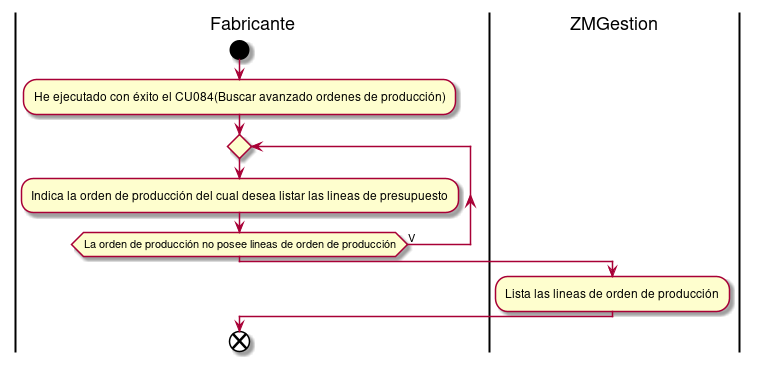
\includegraphics[width=\textwidth,height=0.95\textheight,keepaspectratio]{DiagramasActividad/DiagramaDeActividad/listarLineasOrdenProduccion}
    \caption{CU94 - Listar líneas de orden de producción}
\label{fig:listarLineasOrdenProduccion}
\end{figure}
			%
\renewcommand{\caseUseShortName}{borrarOrdenProduccion} %cammelCase name

\renewcommand{\caseUseCreated}{03/03/2020} %Fecha creación
\renewcommand{\caseUseModified}{03/03/2020} %Fecha modificación
\renewcommand{\caseUseName}{\CUborrarOrdenProduccion - Borrar orden de producción} %{\CUcammelCase - Title}

\renewcommand{\caseUseSummary}{Este caso de uso permite a un administrador de ZMGestion borrar una orden de producción.} %Resumen
\renewcommand{\caseUsePeople}{Administradores: quiere borrar una orden de producción.} %Actor: Meta
\renewcommand{\caseUsePreconditions}{\caseUseRow{Haber realizado con éxito el \CUbuscarAvanzadoOrdenesProduccion\ (Buscar avanzado órdenes de producción).} %Precondiciones
}
\renewcommand{\caseUsePostconditions}{
	\caseUseRow{Ninguna.} %Postcondiciones
}
\renewcommand{\caseUseScene}{ %Escenario principal
    \addCaseUseStep{El administrador indica la orden de producción que desea borrar.}
    \addCaseUseStep{ZMGestion borra la orden de producción y muestra un mensaje indicando el éxito de la operación.}
    \addCaseUseStep{}
    \addCaseUseStep{}
    \addCaseUseStep{}
    \addCaseUseStep{}
    \addCaseUseStep{}
    \addCaseUseStep{}
}
\renewcommand{\alternativeCaseUse}{ %Flujos alternativos
	\newAlternative{A1: La orden de producción no se encuentra en estado `En creación'.}{1} %Flujo alternativo A1.
	\caseUseRow{La secuencia A1 comienza luego del punto 1 del escenario principal.} %¡Indicar número paso!
    \alternativeRow{ZMGestion muestra un mensaje de error indicando que la orden de producción no se encuentra en estado `En creación' y por lo tanto no puede ser borrada.}
    \caseUseRow{El escenario vuelve al punto 1.}
    \caseUseRow{}

}
\renewcommand{\caseUseRequirementsGUI}{
	\caseUseRow{Teclado, Mouse y Pantalla} %Requisitos interfaz de usuario
}
\renewcommand{\caseUseResponseTime}{La interfaz debe responder dentro de un tiempo máximo de 10 segundos.} %Requisitos funcionales: Tiempo de respuesta
\renewcommand{\caseUseConcurrence}{} %Requisitos funcionales: Concurrencia
\renewcommand{\caseUseAvailability}{} %Requisitos funcionales: Disponibilidad

\item Caso de uso \caseUseName
\renewcommand*{\arraystretch}{1.3}
\begin{longtable}[c]{|>{\raggedright}p{0.3\textwidth} | >{\raggedright}p{0.2\textwidth} | p{0.5\textwidth} |}
\caption{\hyperref[sec:listadoCasoUso]{\caseUseName}}
\label{tabla:\caseUseShortName}\\
\hline
\rowcolor{tableCaseUseBackground}

\multicolumn{3}{|l|}{\textcolor{tableCaseUseFontColor}{Descripción textual del caso de uso: \caseUseName}} \\ \hline

Fecha de Creación: & \multicolumn{2}{L{\secondColumnWidth}|}{\caseUseCreated}\\ \hline

Fecha de Modificación: & \multicolumn{2}{L{\secondColumnWidth}|}{\caseUseModified} \\ \hline

Versión: & \multicolumn{2}{L{\secondColumnWidth}|}{1} \\ \hline

Resumen: & \multicolumn{2}{L{\secondColumnWidth}|}{\caseUseSummary} \\ \hline

Personas involucradas y metas: & \multicolumn{2}{L{\secondColumnWidth}|}{\caseUsePeople} \\ \hline

Precondiciones: \caseUsePreconditions \hline

Postcondiciones: \caseUsePostconditions \hline

Escenario principal: \caseUseScene \hline

Flujos alternativos: \alternativeCaseUse \hline

Requisitos de interfaz de usuario: \caseUseRequirementsGUI \hline
\multirow{3}{*}{Requisitos funcionales:}  & Tiempo de respuesta: & \caseUseResponseTime \\ \cline{2-3} 
& Concurrencia: & \caseUseConcurrence \\ \cline{2-3} 
& Disponibilidad: & \caseUseAvailability \\ \hline
\end{longtable}

\setcounter{rownumbers}{0}

\renewcommand{\alternativeCaseUse}{
	\caseUseRow{No existen flujos alternativos.}
}

%DIAGRAMA DE ACTIVIDAD
%\lineabreak[0]
%\activityDiagram{\caseUseShortName}{Diagrama de actividad - \caseUseName}
			%
\renewcommand{\caseUseShortName}{} %cammelCase name

\renewcommand{\caseUseCreated}{15/02/2020} %Fecha creación
\renewcommand{\caseUseModified}{15/02/2020} %Fecha modificación
\renewcommand{\caseUseName}{\CU - } %{\CUcammelCase - Title}

\renewcommand{\caseUseSummary}{} %Resumen
\renewcommand{\caseUsePeople}{} %Actor: Meta
\renewcommand{\caseUsePreconditions}{
	\caseUseRow{Haber iniciado sesión en el sistema.} %Precondiciones
}
\renewcommand{\caseUsePostconditions}{
	\caseUseRow{Ninguna.} %Postcondiciones
}
\renewcommand{\caseUseScene}{ %Escenario principal
    \addCaseUseStep{}
    \addCaseUseStep{}
    \addCaseUseStep{}
    \addCaseUseStep{}
    \addCaseUseStep{}
    \addCaseUseStep{}
    \addCaseUseStep{}
    \addCaseUseStep{}
}
\renewcommand{\alternativeCaseUse}{ %Flujos alternativos
	\newAlternative{A1: Error al .}{NUMERO} %Flujo alternativo A1.
	\caseUseRow{La secuencia A1 comienza luego del punto NUMERO del escenario principal.} %¡Indicar número paso!
    \alternativeRow{}
    \alternativeRow{}
    \alternativeRow{}
    \alternativeRow{}
    \alternativeRow{}
    \alternativeRow{}
    
    \caseUseRow{}

	\newAlternative{A2: Error al .}{NUMERO} %Flujo alternativo A2.
    \caseUseRow{La secuencia A2 comienza luego del punto NUMERO del escenario principal.}%¡Indicar número paso!
    \alternativeRow{}
    \alternativeRow{}
    \alternativeRow{}
    \alternativeRow{}
    \alternativeRow{}
    \alternativeRow{}
}
\renewcommand{\caseUseRequirementsGUI}{
	\caseUseRow{Teclado, Mouse y Pantalla} %Requisitos interfaz de usuario
}
\renewcommand{\caseUseResponseTime}{La interfaz debe responder dentro de un tiempo máximo de 10 segundos.} %Requisitos funcionales: Tiempo de respuesta
\renewcommand{\caseUseConcurrence}{} %Requisitos funcionales: Concurrencia
\renewcommand{\caseUseAvailability}{} %Requisitos funcionales: Disponibilidad

\item Caso de uso \caseUseName
\renewcommand*{\arraystretch}{1.3}
\begin{longtable}[c]{|>{\raggedright}p{0.3\textwidth} | >{\raggedright}p{0.2\textwidth} | p{0.5\textwidth} |}
\caption{\hyperref[sec:listadoCasoUso]{\caseUseName}}
\label{tabla:\caseUseShortName}\\
\hline
\rowcolor{tableCaseUseBackground}

\multicolumn{3}{|l|}{\textcolor{tableCaseUseFontColor}{Descripción textual del caso de uso: \caseUseName}} \\ \hline

Fecha de Creación: & \multicolumn{2}{L{\secondColumnWidth}|}{\caseUseCreated}\\ \hline

Fecha de Modificación: & \multicolumn{2}{L{\secondColumnWidth}|}{\caseUseModified} \\ \hline

Versión: & \multicolumn{2}{L{\secondColumnWidth}|}{1} \\ \hline

Resumen: & \multicolumn{2}{L{\secondColumnWidth}|}{\caseUseSummary} \\ \hline

Personas involucradas y metas: & \multicolumn{2}{L{\secondColumnWidth}|}{\caseUsePeople} \\ \hline

Precondiciones: \caseUsePreconditions \hline

Postcondiciones: \caseUsePostconditions \hline

Escenario principal: \caseUseScene \hline

Flujos alternativos: \alternativeCaseUse \hline

Requisitos de interfaz de usuario: \caseUseRequirementsGUI \hline
\multirow{3}{*}{Requisitos funcionales:}  & Tiempo de respuesta: & \caseUseResponseTime \\ \cline{2-3} 
& Concurrencia: & \caseUseConcurrence \\ \cline{2-3} 
& Disponibilidad: & \caseUseAvailability \\ \hline
\end{longtable}

\setcounter{rownumbers}{0}

\renewcommand{\alternativeCaseUse}{
	\caseUseRow{No existen flujos alternativos.}
}

%DIAGRAMA DE ACTIVIDAD
%\lineabreak[0]
%\activityDiagram{\caseUseShortName}{Diagrama de actividad - \caseUseName}
			%
\renewcommand{\caseUseShortName}{} %cammelCase name

\renewcommand{\caseUseCreated}{15/02/2020} %Fecha creación
\renewcommand{\caseUseModified}{15/02/2020} %Fecha modificación
\renewcommand{\caseUseName}{\CU - } %{\CUcammelCase - Title}

\renewcommand{\caseUseSummary}{} %Resumen
\renewcommand{\caseUsePeople}{} %Actor: Meta
\renewcommand{\caseUsePreconditions}{
	\caseUseRow{Haber iniciado sesión en el sistema.} %Precondiciones
}
\renewcommand{\caseUsePostconditions}{
	\caseUseRow{Ninguna.} %Postcondiciones
}
\renewcommand{\caseUseScene}{ %Escenario principal
    \addCaseUseStep{}
    \addCaseUseStep{}
    \addCaseUseStep{}
    \addCaseUseStep{}
    \addCaseUseStep{}
    \addCaseUseStep{}
    \addCaseUseStep{}
    \addCaseUseStep{}
}
\renewcommand{\alternativeCaseUse}{ %Flujos alternativos
	\newAlternative{A1: Error al .}{NUMERO} %Flujo alternativo A1.
	\caseUseRow{La secuencia A1 comienza luego del punto NUMERO del escenario principal.} %¡Indicar número paso!
    \alternativeRow{}
    \alternativeRow{}
    \alternativeRow{}
    \alternativeRow{}
    \alternativeRow{}
    \alternativeRow{}
    
    \caseUseRow{}

	\newAlternative{A2: Error al .}{NUMERO} %Flujo alternativo A2.
    \caseUseRow{La secuencia A2 comienza luego del punto NUMERO del escenario principal.}%¡Indicar número paso!
    \alternativeRow{}
    \alternativeRow{}
    \alternativeRow{}
    \alternativeRow{}
    \alternativeRow{}
    \alternativeRow{}
}
\renewcommand{\caseUseRequirementsGUI}{
	\caseUseRow{Teclado, Mouse y Pantalla} %Requisitos interfaz de usuario
}
\renewcommand{\caseUseResponseTime}{La interfaz debe responder dentro de un tiempo máximo de 10 segundos.} %Requisitos funcionales: Tiempo de respuesta
\renewcommand{\caseUseConcurrence}{} %Requisitos funcionales: Concurrencia
\renewcommand{\caseUseAvailability}{} %Requisitos funcionales: Disponibilidad

\item Caso de uso \caseUseName
\renewcommand*{\arraystretch}{1.3}
\begin{longtable}[c]{|>{\raggedright}p{0.3\textwidth} | >{\raggedright}p{0.2\textwidth} | p{0.5\textwidth} |}
\caption{\hyperref[sec:listadoCasoUso]{\caseUseName}}
\label{tabla:\caseUseShortName}\\
\hline
\rowcolor{tableCaseUseBackground}

\multicolumn{3}{|l|}{\textcolor{tableCaseUseFontColor}{Descripción textual del caso de uso: \caseUseName}} \\ \hline

Fecha de Creación: & \multicolumn{2}{L{\secondColumnWidth}|}{\caseUseCreated}\\ \hline

Fecha de Modificación: & \multicolumn{2}{L{\secondColumnWidth}|}{\caseUseModified} \\ \hline

Versión: & \multicolumn{2}{L{\secondColumnWidth}|}{1} \\ \hline

Resumen: & \multicolumn{2}{L{\secondColumnWidth}|}{\caseUseSummary} \\ \hline

Personas involucradas y metas: & \multicolumn{2}{L{\secondColumnWidth}|}{\caseUsePeople} \\ \hline

Precondiciones: \caseUsePreconditions \hline

Postcondiciones: \caseUsePostconditions \hline

Escenario principal: \caseUseScene \hline

Flujos alternativos: \alternativeCaseUse \hline

Requisitos de interfaz de usuario: \caseUseRequirementsGUI \hline
\multirow{3}{*}{Requisitos funcionales:}  & Tiempo de respuesta: & \caseUseResponseTime \\ \cline{2-3} 
& Concurrencia: & \caseUseConcurrence \\ \cline{2-3} 
& Disponibilidad: & \caseUseAvailability \\ \hline
\end{longtable}

\setcounter{rownumbers}{0}

\renewcommand{\alternativeCaseUse}{
	\caseUseRow{No existen flujos alternativos.}
}

%DIAGRAMA DE ACTIVIDAD
%\lineabreak[0]
%\activityDiagram{\caseUseShortName}{Diagrama de actividad - \caseUseName}
			%
\renewcommand{\caseUseShortName}{} %cammelCase name

\renewcommand{\caseUseCreated}{15/02/2020} %Fecha creación
\renewcommand{\caseUseModified}{15/02/2020} %Fecha modificación
\renewcommand{\caseUseName}{\CU - } %{\CUcammelCase - Title}

\renewcommand{\caseUseSummary}{} %Resumen
\renewcommand{\caseUsePeople}{} %Actor: Meta
\renewcommand{\caseUsePreconditions}{
	\caseUseRow{Haber iniciado sesión en el sistema.} %Precondiciones
}
\renewcommand{\caseUsePostconditions}{
	\caseUseRow{Ninguna.} %Postcondiciones
}
\renewcommand{\caseUseScene}{ %Escenario principal
    \addCaseUseStep{}
    \addCaseUseStep{}
    \addCaseUseStep{}
    \addCaseUseStep{}
    \addCaseUseStep{}
    \addCaseUseStep{}
    \addCaseUseStep{}
    \addCaseUseStep{}
}
\renewcommand{\alternativeCaseUse}{ %Flujos alternativos
	\newAlternative{A1: Error al .}{NUMERO} %Flujo alternativo A1.
	\caseUseRow{La secuencia A1 comienza luego del punto NUMERO del escenario principal.} %¡Indicar número paso!
    \alternativeRow{}
    \alternativeRow{}
    \alternativeRow{}
    \alternativeRow{}
    \alternativeRow{}
    \alternativeRow{}
    
    \caseUseRow{}

	\newAlternative{A2: Error al .}{NUMERO} %Flujo alternativo A2.
    \caseUseRow{La secuencia A2 comienza luego del punto NUMERO del escenario principal.}%¡Indicar número paso!
    \alternativeRow{}
    \alternativeRow{}
    \alternativeRow{}
    \alternativeRow{}
    \alternativeRow{}
    \alternativeRow{}
}
\renewcommand{\caseUseRequirementsGUI}{
	\caseUseRow{Teclado, Mouse y Pantalla} %Requisitos interfaz de usuario
}
\renewcommand{\caseUseResponseTime}{La interfaz debe responder dentro de un tiempo máximo de 10 segundos.} %Requisitos funcionales: Tiempo de respuesta
\renewcommand{\caseUseConcurrence}{} %Requisitos funcionales: Concurrencia
\renewcommand{\caseUseAvailability}{} %Requisitos funcionales: Disponibilidad

\item Caso de uso \caseUseName
\renewcommand*{\arraystretch}{1.3}
\begin{longtable}[c]{|>{\raggedright}p{0.3\textwidth} | >{\raggedright}p{0.2\textwidth} | p{0.5\textwidth} |}
\caption{\hyperref[sec:listadoCasoUso]{\caseUseName}}
\label{tabla:\caseUseShortName}\\
\hline
\rowcolor{tableCaseUseBackground}

\multicolumn{3}{|l|}{\textcolor{tableCaseUseFontColor}{Descripción textual del caso de uso: \caseUseName}} \\ \hline

Fecha de Creación: & \multicolumn{2}{L{\secondColumnWidth}|}{\caseUseCreated}\\ \hline

Fecha de Modificación: & \multicolumn{2}{L{\secondColumnWidth}|}{\caseUseModified} \\ \hline

Versión: & \multicolumn{2}{L{\secondColumnWidth}|}{1} \\ \hline

Resumen: & \multicolumn{2}{L{\secondColumnWidth}|}{\caseUseSummary} \\ \hline

Personas involucradas y metas: & \multicolumn{2}{L{\secondColumnWidth}|}{\caseUsePeople} \\ \hline

Precondiciones: \caseUsePreconditions \hline

Postcondiciones: \caseUsePostconditions \hline

Escenario principal: \caseUseScene \hline

Flujos alternativos: \alternativeCaseUse \hline

Requisitos de interfaz de usuario: \caseUseRequirementsGUI \hline
\multirow{3}{*}{Requisitos funcionales:}  & Tiempo de respuesta: & \caseUseResponseTime \\ \cline{2-3} 
& Concurrencia: & \caseUseConcurrence \\ \cline{2-3} 
& Disponibilidad: & \caseUseAvailability \\ \hline
\end{longtable}

\setcounter{rownumbers}{0}

\renewcommand{\alternativeCaseUse}{
	\caseUseRow{No existen flujos alternativos.}
}

%DIAGRAMA DE ACTIVIDAD
%\lineabreak[0]
%\activityDiagram{\caseUseShortName}{Diagrama de actividad - \caseUseName}
			%
\renewcommand{\caseUseShortName}{cancelarOrdenProduccion} %cammelCase name

\renewcommand{\caseUseCreated}{05/03/2020} %Fecha creación
\renewcommand{\caseUseModified}{05/03/2020} %Fecha modificación
\renewcommand{\caseUseName}{\CUcancelarOrdenProduccion - Cancelar orden de producción} %{\CUcammelCase - Title}

\renewcommand{\caseUseSummary}{Este caso de uso permite a un administrador de ZMGestion cancelar una orden de producción.} %Resumen
\renewcommand{\caseUsePeople}{Administradores: quiere cancelar una orden de producción existente.} %Actor: Meta
\renewcommand{\caseUsePreconditions}{
	\caseUseRow{Haber realizado con éxito el \CUbuscarAvanzadoOrdenesProduccion\ (Buscar avanzado órdenes de producción).}
}
\renewcommand{\caseUsePostconditions}{
	\caseUseRow{Ninguna.} %Postcondiciones
}
\renewcommand{\caseUseScene}{ %Escenario principal
    \addCaseUseStep{El administrador selecciona una orden de producción que desea cancelar.}
    \addCaseUseStep{ZMGestion ejecuta el \CUcancelarLineaOrdenProduccion\ (Cancelar línea orden de producción) para cada línea de la orden de producción que se encuentre `Pendiente de producción' o `En producción'.}
}
\renewcommand{\alternativeCaseUse}{ %Flujos alternativos
	\newAlternative{A1: La orden de producción seleccionada no se encuentra en estado `Pendiente' o `En producción'.}{1} %Flujo alternativo A1.
	\caseUseRow{La secuencia A1 comienza luego del punto 1 del escenario principal.} %¡Indicar número paso!
    \alternativeRow{ZMGestion muestra un mensaje de error indicando que la orden de producción no puede cancelarse.}
    \caseUseRow{El escenario vuelve al punto 1.}
    \caseUseRow{}
}

%\item Caso de uso \caseUseName
\renewcommand*{\arraystretch}{1.3}
\begin{longtable}[c]{|>{\raggedright}p{0.3\textwidth} | >{\raggedright}p{0.2\textwidth} | p{0.5\textwidth} |}
\caption{\hyperref[sec:listadoCasoUso]{\caseUseName}}
\label{tabla:\caseUseShortName}\\
\hline
\rowcolor{tableCaseUseBackground}

\multicolumn{3}{|l|}{\textcolor{tableCaseUseFontColor}{Descripción textual del caso de uso: \caseUseName}} \\ \hline

Fecha de Creación: & \multicolumn{2}{L{\secondColumnWidth}|}{\caseUseCreated}\\ \hline

Fecha de Modificación: & \multicolumn{2}{L{\secondColumnWidth}|}{\caseUseModified} \\ \hline

Versión: & \multicolumn{2}{L{\secondColumnWidth}|}{1} \\ \hline

Resumen: & \multicolumn{2}{L{\secondColumnWidth}|}{\caseUseSummary} \\ \hline

Personas involucradas y metas: & \multicolumn{2}{L{\secondColumnWidth}|}{\caseUsePeople} \\ \hline

Precondiciones: \caseUsePreconditions \hline

Postcondiciones: \caseUsePostconditions \hline

Escenario principal: \caseUseScene \hline

Flujos alternativos: \alternativeCaseUse \hline

Requisitos de interfaz de usuario: \caseUseRequirementsGUI \hline
\multirow{3}{*}{Requisitos funcionales:}  & Tiempo de respuesta: & \caseUseResponseTime \\ \cline{2-3} 
& Concurrencia: & \caseUseConcurrence \\ \cline{2-3} 
& Disponibilidad: & \caseUseAvailability \\ \hline
\end{longtable}

\setcounter{rownumbers}{0}

\renewcommand{\alternativeCaseUse}{
	\caseUseRow{No existen flujos alternativos.}
}

%DIAGRAMA DE ACTIVIDAD
%\lineabreak[0]
\activityDiagram{\caseUseShortName}{Diagrama de actividad - \caseUseName}
			%\renewcommand{\caseUseShortName}{listarObservacionesLineaOrdenProduccion} %cammelCase name
\renewcommand{\caseUseCreated}{05/03/2020} %Fecha creación
\renewcommand{\caseUseModified}{05/03/2020} %Fecha modificación
\renewcommand{\caseUseName}{\CUlistarObservacionesLineaOrdenProduccion - Listar observaciones de línea de orden de producción.} %{\CUcammelCase - Title}

\renewcommand{\caseUseSummary}{Este caso de uso permite a los fabricantes de ZMGestion listar las observaciones de una línea de orden de producción.} %Resumen
\renewcommand{\caseUsePeople}{Fabricantes: quiere listar las observaciones de una linea de orden de producción.} %Actor: Meta
\renewcommand{\caseUsePreconditions}{\caseUseRow{Haber realizado con éxito el \CUlistarLineasOrdenProduccion\ (Listar líneas de orden de producción).} %Precondiciones
}
\renewcommand{\caseUsePostconditions}{
	\caseUseRow{Ninguna.} %Postcondiciones
}
\renewcommand{\caseUseScene}{ %Escenario principal
    \addCaseUseStep{El fabricante selecciona una línea de orden de producción a la cual le desea listar sus observaciones.}
    \addCaseUseStep{ZMGestion lista las observaciones de la línea de orden de producción seleccionada.}
}
\renewcommand{\alternativeCaseUse}{ %Flujos alternativos
	\newAlternative{A1: La línea de orden de producción no posee observaciones.}{1} %Flujo alternativo A1.
	\caseUseRow{La secuencia A1 comienza luego del punto 1 del escenario principal.} %¡Indicar número paso!
    \alternativeRow{ZMGestion muestra un mensaje indicando que la línea de orden de producción no posee observaciones.}
    \caseUseRow{El escenario vuelve al punto 1.}
    \caseUseRow{}
}

\item Caso de uso \caseUseName
\renewcommand*{\arraystretch}{1.3}
\begin{longtable}[c]{|>{\raggedright}p{0.3\textwidth} | >{\raggedright}p{0.2\textwidth} | p{0.5\textwidth} |}
\caption{\hyperref[sec:listadoCasoUso]{\caseUseName}}
\label{tabla:\caseUseShortName}\\
\hline
\rowcolor{tableCaseUseBackground}

\multicolumn{3}{|l|}{\textcolor{tableCaseUseFontColor}{Descripción textual del caso de uso: \caseUseName}} \\ \hline

Fecha de Creación: & \multicolumn{2}{L{\secondColumnWidth}|}{\caseUseCreated}\\ \hline

Fecha de Modificación: & \multicolumn{2}{L{\secondColumnWidth}|}{\caseUseModified} \\ \hline

Versión: & \multicolumn{2}{L{\secondColumnWidth}|}{1} \\ \hline

Resumen: & \multicolumn{2}{L{\secondColumnWidth}|}{\caseUseSummary} \\ \hline

Personas involucradas y metas: & \multicolumn{2}{L{\secondColumnWidth}|}{\caseUsePeople} \\ \hline

Precondiciones: \caseUsePreconditions \hline

Postcondiciones: \caseUsePostconditions \hline

Escenario principal: \caseUseScene \hline

Flujos alternativos: \alternativeCaseUse \hline

Requisitos de interfaz de usuario: \caseUseRequirementsGUI \hline
\multirow{3}{*}{Requisitos funcionales:}  & Tiempo de respuesta: & \caseUseResponseTime \\ \cline{2-3} 
& Concurrencia: & \caseUseConcurrence \\ \cline{2-3} 
& Disponibilidad: & \caseUseAvailability \\ \hline
\end{longtable}

\setcounter{rownumbers}{0}

\renewcommand{\alternativeCaseUse}{
	\caseUseRow{No existen flujos alternativos.}
}

%DIAGRAMA DE ACTIVIDAD
%\lineabreak[0]
%\activityDiagram{\caseUseShortName}{Diagrama de actividad - \caseUseName}

			%GestionLineasOrdenesProduccion
			%
\renewcommand{\caseUseShortName}{} %cammelCase name

\renewcommand{\caseUseCreated}{15/02/2020} %Fecha creación
\renewcommand{\caseUseModified}{15/02/2020} %Fecha modificación
\renewcommand{\caseUseName}{\CU - } %{\CUcammelCase - Title}

\renewcommand{\caseUseSummary}{} %Resumen
\renewcommand{\caseUsePeople}{} %Actor: Meta
\renewcommand{\caseUsePreconditions}{
	\caseUseRow{Haber iniciado sesión en el sistema.} %Precondiciones
}
\renewcommand{\caseUsePostconditions}{
	\caseUseRow{Ninguna.} %Postcondiciones
}
\renewcommand{\caseUseScene}{ %Escenario principal
    \addCaseUseStep{}
    \addCaseUseStep{}
    \addCaseUseStep{}
    \addCaseUseStep{}
    \addCaseUseStep{}
    \addCaseUseStep{}
    \addCaseUseStep{}
    \addCaseUseStep{}
}
\renewcommand{\alternativeCaseUse}{ %Flujos alternativos
	\newAlternative{A1: Error al .}{NUMERO} %Flujo alternativo A1.
	\caseUseRow{La secuencia A1 comienza luego del punto NUMERO del escenario principal.} %¡Indicar número paso!
    \alternativeRow{}
    \alternativeRow{}
    \alternativeRow{}
    \alternativeRow{}
    \alternativeRow{}
    \alternativeRow{}
    
    \caseUseRow{}

	\newAlternative{A2: Error al .}{NUMERO} %Flujo alternativo A2.
    \caseUseRow{La secuencia A2 comienza luego del punto NUMERO del escenario principal.}%¡Indicar número paso!
    \alternativeRow{}
    \alternativeRow{}
    \alternativeRow{}
    \alternativeRow{}
    \alternativeRow{}
    \alternativeRow{}
}
\renewcommand{\caseUseRequirementsGUI}{
	\caseUseRow{Teclado, Mouse y Pantalla} %Requisitos interfaz de usuario
}
\renewcommand{\caseUseResponseTime}{La interfaz debe responder dentro de un tiempo máximo de 10 segundos.} %Requisitos funcionales: Tiempo de respuesta
\renewcommand{\caseUseConcurrence}{} %Requisitos funcionales: Concurrencia
\renewcommand{\caseUseAvailability}{} %Requisitos funcionales: Disponibilidad

\item Caso de uso \caseUseName
\renewcommand*{\arraystretch}{1.3}
\begin{longtable}[c]{|>{\raggedright}p{0.3\textwidth} | >{\raggedright}p{0.2\textwidth} | p{0.5\textwidth} |}
\caption{\hyperref[sec:listadoCasoUso]{\caseUseName}}
\label{tabla:\caseUseShortName}\\
\hline
\rowcolor{tableCaseUseBackground}

\multicolumn{3}{|l|}{\textcolor{tableCaseUseFontColor}{Descripción textual del caso de uso: \caseUseName}} \\ \hline

Fecha de Creación: & \multicolumn{2}{L{\secondColumnWidth}|}{\caseUseCreated}\\ \hline

Fecha de Modificación: & \multicolumn{2}{L{\secondColumnWidth}|}{\caseUseModified} \\ \hline

Versión: & \multicolumn{2}{L{\secondColumnWidth}|}{1} \\ \hline

Resumen: & \multicolumn{2}{L{\secondColumnWidth}|}{\caseUseSummary} \\ \hline

Personas involucradas y metas: & \multicolumn{2}{L{\secondColumnWidth}|}{\caseUsePeople} \\ \hline

Precondiciones: \caseUsePreconditions \hline

Postcondiciones: \caseUsePostconditions \hline

Escenario principal: \caseUseScene \hline

Flujos alternativos: \alternativeCaseUse \hline

Requisitos de interfaz de usuario: \caseUseRequirementsGUI \hline
\multirow{3}{*}{Requisitos funcionales:}  & Tiempo de respuesta: & \caseUseResponseTime \\ \cline{2-3} 
& Concurrencia: & \caseUseConcurrence \\ \cline{2-3} 
& Disponibilidad: & \caseUseAvailability \\ \hline
\end{longtable}

\setcounter{rownumbers}{0}

\renewcommand{\alternativeCaseUse}{
	\caseUseRow{No existen flujos alternativos.}
}

%DIAGRAMA DE ACTIVIDAD
%\lineabreak[0]
%\activityDiagram{\caseUseShortName}{Diagrama de actividad - \caseUseName}
			%
\renewcommand{\caseUseShortName}{modificarLineaOrdenProduccion} %cammelCase name

\renewcommand{\caseUseCreated}{04/03/2020} %Fecha creación
\renewcommand{\caseUseModified}{04/03/2020} %Fecha modificación
\renewcommand{\caseUseName}{\CUmodificarLineaOrdenProduccion - Modificar línea de orden de producción} %{\CUcammelCase - Title}

\renewcommand{\caseUseSummary}{Este caso de uso permite a un administrador de ZMGestion modificar una línea de orden de producción.} %Resumen
\renewcommand{\caseUsePeople}{Administradores: desea modificar una línea de orden de producción.} %Actor: Meta
\renewcommand{\caseUsePreconditions}{
	\caseUseRow{Haber ejecutado con éxito el \CUlistarLineasOrdenProduccion (Listar lineas de orden de producción).} %Precondiciones
}
\renewcommand{\caseUsePostconditions}{
	\caseUseRow{Ninguna.} %Postcondiciones
}
\renewcommand{\caseUseScene}{ %Escenario principal
    \addCaseUseStep{El administrador indica la línea de orden de producción que desea modificar.}
    \addCaseUseStep{ZMGestion muestra un formulario autocompletado con los datos de la linea de orden de producción seleccionada, producto, tela, lustre y cantidad a producirse. Indicando que el producto y la cantidad son obligatorios.}
    \addCaseUseStep{El administrador modifica el formulario.}
    \addCaseUseStep{ZMGestion modifica la línea de orden de producción y muestra un mensaje indicando el éxito de la operación.}

}
\renewcommand{\alternativeCaseUse}{ %Flujos alternativos
	\newAlternative{A1: La línea de orden de producción seleccionada no se encuentra en estado de `Pendiente de producción'.}{1} %Flujo alternativo A1.
	\caseUseRow{La secuencia A1 comienza luego del punto 1 del escenario principal.} %¡Indicar número paso!
    \alternativeRow{ZMgestion muestra un mensaje de error indicando que la línea de orden de producción no puede modificarse.}
    \caseUseRow{El escenario vuelve al punto 1.}
    \caseUseRow{}

	\newAlternative{A2: La cantidad a producirse es menor o igual que cero.}{3} %Flujo alternativo A2.
    \caseUseRow{La secuencia A2 comienza luego del punto 3 del escenario principal.}%¡Indicar número paso!
    \alternativeRow{ZMGestion muestra un mensaje de error indicando que la cantidad a producirse debe ser mayor que cero.}
    \caseUseRow{El escenario vuelve al punto 2.}
    \caseUseRow{}

    \newAlternative{A3: Existe una línea de orden de producción, producto, tela y lustre, igual en la orden de producción.}{3} %Flujo alternativo A2.
    \caseUseRow{La secuencia A3 comienza luego del punto 3 del escenario principal.}%¡Indicar número paso!
    \alternativeRow{ZMGestion muestra un mensaje de error indicando que ya existe una línea de orden de producción identica en la orden de producción.}
    \caseUseRow{El escenario vuelve al punto 2.}
    \caseUseRow{}

    \newAlternative{A4: El tipo de producto seleccionado no es del tipo `Producible'.}{3} %Flujo alternativo A4.
    \caseUseRow{La secuencia A4 comienza luego del punto 3 del escenario principal.} %¡Indicar número paso!
    \alternativeRow{ZMGestion muestra un mensaje de error indicando que el producto seleccionado no puede ser asignado a una orden de producción.}
    \caseUseRow{El escenario vuelve al punto 2.}
    \caseUseRow{}

    \newAlternative{A5: El administrador ha dejado un campo obligatorio vacio.}{3} %Flujo alternativo A1.
    \caseUseRow{La secuencia A5 comienza luego del punto 3 del escenario principal.} %¡Indicar número paso!
    \alternativeRow{ZMGestion muestra un mensaje de error indicando que ha dejado un campo obligatorio vacio.}
    \caseUseRow{El escenario vuelve al punto 2.}
    \caseUseRow{}
}

\item Caso de uso \caseUseName
\renewcommand*{\arraystretch}{1.3}
\begin{longtable}[c]{|>{\raggedright}p{0.3\textwidth} | >{\raggedright}p{0.2\textwidth} | p{0.5\textwidth} |}
\caption{\hyperref[sec:listadoCasoUso]{\caseUseName}}
\label{tabla:\caseUseShortName}\\
\hline
\rowcolor{tableCaseUseBackground}

\multicolumn{3}{|l|}{\textcolor{tableCaseUseFontColor}{Descripción textual del caso de uso: \caseUseName}} \\ \hline

Fecha de Creación: & \multicolumn{2}{L{\secondColumnWidth}|}{\caseUseCreated}\\ \hline

Fecha de Modificación: & \multicolumn{2}{L{\secondColumnWidth}|}{\caseUseModified} \\ \hline

Versión: & \multicolumn{2}{L{\secondColumnWidth}|}{1} \\ \hline

Resumen: & \multicolumn{2}{L{\secondColumnWidth}|}{\caseUseSummary} \\ \hline

Personas involucradas y metas: & \multicolumn{2}{L{\secondColumnWidth}|}{\caseUsePeople} \\ \hline

Precondiciones: \caseUsePreconditions \hline

Postcondiciones: \caseUsePostconditions \hline

Escenario principal: \caseUseScene \hline

Flujos alternativos: \alternativeCaseUse \hline

Requisitos de interfaz de usuario: \caseUseRequirementsGUI \hline
\multirow{3}{*}{Requisitos funcionales:}  & Tiempo de respuesta: & \caseUseResponseTime \\ \cline{2-3} 
& Concurrencia: & \caseUseConcurrence \\ \cline{2-3} 
& Disponibilidad: & \caseUseAvailability \\ \hline
\end{longtable}

\setcounter{rownumbers}{0}

\renewcommand{\alternativeCaseUse}{
	\caseUseRow{No existen flujos alternativos.}
}

%DIAGRAMA DE ACTIVIDAD
%\lineabreak[0]
%\activityDiagram{\caseUseShortName}{Diagrama de actividad - \caseUseName}
			%
\renewcommand{\caseUseShortName}{} %cammelCase name

\renewcommand{\caseUseCreated}{15/02/2020} %Fecha creación
\renewcommand{\caseUseModified}{15/02/2020} %Fecha modificación
\renewcommand{\caseUseName}{\CU - } %{\CUcammelCase - Title}

\renewcommand{\caseUseSummary}{} %Resumen
\renewcommand{\caseUsePeople}{} %Actor: Meta
\renewcommand{\caseUsePreconditions}{
	\caseUseRow{Haber iniciado sesión en el sistema.} %Precondiciones
}
\renewcommand{\caseUsePostconditions}{
	\caseUseRow{Ninguna.} %Postcondiciones
}
\renewcommand{\caseUseScene}{ %Escenario principal
    \addCaseUseStep{}
    \addCaseUseStep{}
    \addCaseUseStep{}
    \addCaseUseStep{}
    \addCaseUseStep{}
    \addCaseUseStep{}
    \addCaseUseStep{}
    \addCaseUseStep{}
}
\renewcommand{\alternativeCaseUse}{ %Flujos alternativos
	\newAlternative{A1: Error al .}{NUMERO} %Flujo alternativo A1.
	\caseUseRow{La secuencia A1 comienza luego del punto NUMERO del escenario principal.} %¡Indicar número paso!
    \alternativeRow{}
    \alternativeRow{}
    \alternativeRow{}
    \alternativeRow{}
    \alternativeRow{}
    \alternativeRow{}
    
    \caseUseRow{}

	\newAlternative{A2: Error al .}{NUMERO} %Flujo alternativo A2.
    \caseUseRow{La secuencia A2 comienza luego del punto NUMERO del escenario principal.}%¡Indicar número paso!
    \alternativeRow{}
    \alternativeRow{}
    \alternativeRow{}
    \alternativeRow{}
    \alternativeRow{}
    \alternativeRow{}
}
\renewcommand{\caseUseRequirementsGUI}{
	\caseUseRow{Teclado, Mouse y Pantalla} %Requisitos interfaz de usuario
}
\renewcommand{\caseUseResponseTime}{La interfaz debe responder dentro de un tiempo máximo de 10 segundos.} %Requisitos funcionales: Tiempo de respuesta
\renewcommand{\caseUseConcurrence}{} %Requisitos funcionales: Concurrencia
\renewcommand{\caseUseAvailability}{} %Requisitos funcionales: Disponibilidad

\item Caso de uso \caseUseName
\renewcommand*{\arraystretch}{1.3}
\begin{longtable}[c]{|>{\raggedright}p{0.3\textwidth} | >{\raggedright}p{0.2\textwidth} | p{0.5\textwidth} |}
\caption{\hyperref[sec:listadoCasoUso]{\caseUseName}}
\label{tabla:\caseUseShortName}\\
\hline
\rowcolor{tableCaseUseBackground}

\multicolumn{3}{|l|}{\textcolor{tableCaseUseFontColor}{Descripción textual del caso de uso: \caseUseName}} \\ \hline

Fecha de Creación: & \multicolumn{2}{L{\secondColumnWidth}|}{\caseUseCreated}\\ \hline

Fecha de Modificación: & \multicolumn{2}{L{\secondColumnWidth}|}{\caseUseModified} \\ \hline

Versión: & \multicolumn{2}{L{\secondColumnWidth}|}{1} \\ \hline

Resumen: & \multicolumn{2}{L{\secondColumnWidth}|}{\caseUseSummary} \\ \hline

Personas involucradas y metas: & \multicolumn{2}{L{\secondColumnWidth}|}{\caseUsePeople} \\ \hline

Precondiciones: \caseUsePreconditions \hline

Postcondiciones: \caseUsePostconditions \hline

Escenario principal: \caseUseScene \hline

Flujos alternativos: \alternativeCaseUse \hline

Requisitos de interfaz de usuario: \caseUseRequirementsGUI \hline
\multirow{3}{*}{Requisitos funcionales:}  & Tiempo de respuesta: & \caseUseResponseTime \\ \cline{2-3} 
& Concurrencia: & \caseUseConcurrence \\ \cline{2-3} 
& Disponibilidad: & \caseUseAvailability \\ \hline
\end{longtable}

\setcounter{rownumbers}{0}

\renewcommand{\alternativeCaseUse}{
	\caseUseRow{No existen flujos alternativos.}
}

%DIAGRAMA DE ACTIVIDAD
%\lineabreak[0]
%\activityDiagram{\caseUseShortName}{Diagrama de actividad - \caseUseName}
			%
\renewcommand{\caseUseShortName}{} %cammelCase name

\renewcommand{\caseUseCreated}{15/02/2020} %Fecha creación
\renewcommand{\caseUseModified}{15/02/2020} %Fecha modificación
\renewcommand{\caseUseName}{\CU - } %{\CUcammelCase - Title}

\renewcommand{\caseUseSummary}{} %Resumen
\renewcommand{\caseUsePeople}{} %Actor: Meta
\renewcommand{\caseUsePreconditions}{
	\caseUseRow{Haber iniciado sesión en el sistema.} %Precondiciones
}
\renewcommand{\caseUsePostconditions}{
	\caseUseRow{Ninguna.} %Postcondiciones
}
\renewcommand{\caseUseScene}{ %Escenario principal
    \addCaseUseStep{}
    \addCaseUseStep{}
    \addCaseUseStep{}
    \addCaseUseStep{}
    \addCaseUseStep{}
    \addCaseUseStep{}
    \addCaseUseStep{}
    \addCaseUseStep{}
}
\renewcommand{\alternativeCaseUse}{ %Flujos alternativos
	\newAlternative{A1: Error al .}{NUMERO} %Flujo alternativo A1.
	\caseUseRow{La secuencia A1 comienza luego del punto NUMERO del escenario principal.} %¡Indicar número paso!
    \alternativeRow{}
    \alternativeRow{}
    \alternativeRow{}
    \alternativeRow{}
    \alternativeRow{}
    \alternativeRow{}
    
    \caseUseRow{}

	\newAlternative{A2: Error al .}{NUMERO} %Flujo alternativo A2.
    \caseUseRow{La secuencia A2 comienza luego del punto NUMERO del escenario principal.}%¡Indicar número paso!
    \alternativeRow{}
    \alternativeRow{}
    \alternativeRow{}
    \alternativeRow{}
    \alternativeRow{}
    \alternativeRow{}
}
\renewcommand{\caseUseRequirementsGUI}{
	\caseUseRow{Teclado, Mouse y Pantalla} %Requisitos interfaz de usuario
}
\renewcommand{\caseUseResponseTime}{La interfaz debe responder dentro de un tiempo máximo de 10 segundos.} %Requisitos funcionales: Tiempo de respuesta
\renewcommand{\caseUseConcurrence}{} %Requisitos funcionales: Concurrencia
\renewcommand{\caseUseAvailability}{} %Requisitos funcionales: Disponibilidad

\item Caso de uso \caseUseName
\renewcommand*{\arraystretch}{1.3}
\begin{longtable}[c]{|>{\raggedright}p{0.3\textwidth} | >{\raggedright}p{0.2\textwidth} | p{0.5\textwidth} |}
\caption{\hyperref[sec:listadoCasoUso]{\caseUseName}}
\label{tabla:\caseUseShortName}\\
\hline
\rowcolor{tableCaseUseBackground}

\multicolumn{3}{|l|}{\textcolor{tableCaseUseFontColor}{Descripción textual del caso de uso: \caseUseName}} \\ \hline

Fecha de Creación: & \multicolumn{2}{L{\secondColumnWidth}|}{\caseUseCreated}\\ \hline

Fecha de Modificación: & \multicolumn{2}{L{\secondColumnWidth}|}{\caseUseModified} \\ \hline

Versión: & \multicolumn{2}{L{\secondColumnWidth}|}{1} \\ \hline

Resumen: & \multicolumn{2}{L{\secondColumnWidth}|}{\caseUseSummary} \\ \hline

Personas involucradas y metas: & \multicolumn{2}{L{\secondColumnWidth}|}{\caseUsePeople} \\ \hline

Precondiciones: \caseUsePreconditions \hline

Postcondiciones: \caseUsePostconditions \hline

Escenario principal: \caseUseScene \hline

Flujos alternativos: \alternativeCaseUse \hline

Requisitos de interfaz de usuario: \caseUseRequirementsGUI \hline
\multirow{3}{*}{Requisitos funcionales:}  & Tiempo de respuesta: & \caseUseResponseTime \\ \cline{2-3} 
& Concurrencia: & \caseUseConcurrence \\ \cline{2-3} 
& Disponibilidad: & \caseUseAvailability \\ \hline
\end{longtable}

\setcounter{rownumbers}{0}

\renewcommand{\alternativeCaseUse}{
	\caseUseRow{No existen flujos alternativos.}
}

%DIAGRAMA DE ACTIVIDAD
%\lineabreak[0]
%\activityDiagram{\caseUseShortName}{Diagrama de actividad - \caseUseName}
			%
\renewcommand{\caseUseShortName}{verificarLineaOrdenProduccion} %cammelCase name

\renewcommand{\caseUseCreated}{04/03/2020} %Fecha creación
\renewcommand{\caseUseModified}{04/03/2020} %Fecha modificación
\renewcommand{\caseUseName}{\CUverificarLineaOrdenProduccion - Verificar línea de orden de producción} %{\CUcammelCase - Title}

\renewcommand{\caseUseSummary}{Este caso de uso permite a un administrador de ZMGestion verificar que una línea de orden de producción (cuyas tareas se encuentran finalizadas) efectivamente se ha finalizado.} %Resumen
\renewcommand{\caseUsePeople}{Administradores: quiere verificar que una línea de orden de producción está finalizada.} %Actor: Meta
\renewcommand{\caseUsePreconditions}{
	\caseUseRow{Haber ejecutado con éxito el \CUlistarLineasOrdenProduccion (Listar lineas de orden de producción).} %Precondiciones
}
\renewcommand{\caseUsePostconditions}{
	\caseUseRow{Ninguna.} %Postcondiciones
}
\renewcommand{\caseUseScene}{ %Escenario principal
    \addCaseUseStep{El administrador indica la línea de orden de producción que desea verificar que esta finalizada.}
    \addCaseUseStep{ZMGestion pasa la línea de orden de producción al estado `Verificada' y en caso de tener una venta asociada reserva los productos fabricados para el cliente, pasando las lineas de venta utilizadas para generar la orden de produccion al estado `Reservada'.}
}
\renewcommand{\alternativeCaseUse}{ %Flujos alternativos
	\newAlternative{A1: La línea de orden de producción no se encuentra en estado `En producción' o sus tareas no están todas finalizadas.}{1} %Flujo alternativoA1.
	\caseUseRow{La secuencia A1 comienza luego del punto 1 del escenario principal.} %¡Indicar número paso!
    \alternativeRow{ZMGestion muestra un mensaje de error indicando que la línea de orden de producción no puede ser verificada.}
    \caseUseRow{El escenario vuelve al punto 1.}    
    \caseUseRow{}
}

%\item Caso de uso \caseUseName
\renewcommand*{\arraystretch}{1.3}
\begin{longtable}[c]{|>{\raggedright}p{0.3\textwidth} | >{\raggedright}p{0.2\textwidth} | p{0.5\textwidth} |}
\caption{\hyperref[sec:listadoCasoUso]{\caseUseName}}
\label{tabla:\caseUseShortName}\\
\hline
\rowcolor{tableCaseUseBackground}

\multicolumn{3}{|l|}{\textcolor{tableCaseUseFontColor}{Descripción textual del caso de uso: \caseUseName}} \\ \hline

Fecha de Creación: & \multicolumn{2}{L{\secondColumnWidth}|}{\caseUseCreated}\\ \hline

Fecha de Modificación: & \multicolumn{2}{L{\secondColumnWidth}|}{\caseUseModified} \\ \hline

Versión: & \multicolumn{2}{L{\secondColumnWidth}|}{1} \\ \hline

Resumen: & \multicolumn{2}{L{\secondColumnWidth}|}{\caseUseSummary} \\ \hline

Personas involucradas y metas: & \multicolumn{2}{L{\secondColumnWidth}|}{\caseUsePeople} \\ \hline

Precondiciones: \caseUsePreconditions \hline

Postcondiciones: \caseUsePostconditions \hline

Escenario principal: \caseUseScene \hline

Flujos alternativos: \alternativeCaseUse \hline

Requisitos de interfaz de usuario: \caseUseRequirementsGUI \hline
\multirow{3}{*}{Requisitos funcionales:}  & Tiempo de respuesta: & \caseUseResponseTime \\ \cline{2-3} 
& Concurrencia: & \caseUseConcurrence \\ \cline{2-3} 
& Disponibilidad: & \caseUseAvailability \\ \hline
\end{longtable}

\setcounter{rownumbers}{0}

\renewcommand{\alternativeCaseUse}{
	\caseUseRow{No existen flujos alternativos.}
}

%DIAGRAMA DE ACTIVIDAD
%\lineabreak[0]
%\activityDiagram{\caseUseShortName}{Diagrama de actividad - \caseUseName}
			%
\renewcommand{\caseUseShortName}{} %cammelCase name

\renewcommand{\caseUseCreated}{15/02/2020} %Fecha creación
\renewcommand{\caseUseModified}{15/02/2020} %Fecha modificación
\renewcommand{\caseUseName}{\CU - } %{\CUcammelCase - Title}

\renewcommand{\caseUseSummary}{} %Resumen
\renewcommand{\caseUsePeople}{} %Actor: Meta
\renewcommand{\caseUsePreconditions}{
	\caseUseRow{Haber iniciado sesión en el sistema.} %Precondiciones
}
\renewcommand{\caseUsePostconditions}{
	\caseUseRow{Ninguna.} %Postcondiciones
}
\renewcommand{\caseUseScene}{ %Escenario principal
    \addCaseUseStep{}
    \addCaseUseStep{}
    \addCaseUseStep{}
    \addCaseUseStep{}
    \addCaseUseStep{}
    \addCaseUseStep{}
    \addCaseUseStep{}
    \addCaseUseStep{}
}
\renewcommand{\alternativeCaseUse}{ %Flujos alternativos
	\newAlternative{A1: Error al .}{NUMERO} %Flujo alternativo A1.
	\caseUseRow{La secuencia A1 comienza luego del punto NUMERO del escenario principal.} %¡Indicar número paso!
    \alternativeRow{}
    \alternativeRow{}
    \alternativeRow{}
    \alternativeRow{}
    \alternativeRow{}
    \alternativeRow{}
    
    \caseUseRow{}

	\newAlternative{A2: Error al .}{NUMERO} %Flujo alternativo A2.
    \caseUseRow{La secuencia A2 comienza luego del punto NUMERO del escenario principal.}%¡Indicar número paso!
    \alternativeRow{}
    \alternativeRow{}
    \alternativeRow{}
    \alternativeRow{}
    \alternativeRow{}
    \alternativeRow{}
}
\renewcommand{\caseUseRequirementsGUI}{
	\caseUseRow{Teclado, Mouse y Pantalla} %Requisitos interfaz de usuario
}
\renewcommand{\caseUseResponseTime}{La interfaz debe responder dentro de un tiempo máximo de 10 segundos.} %Requisitos funcionales: Tiempo de respuesta
\renewcommand{\caseUseConcurrence}{} %Requisitos funcionales: Concurrencia
\renewcommand{\caseUseAvailability}{} %Requisitos funcionales: Disponibilidad

\item Caso de uso \caseUseName
\renewcommand*{\arraystretch}{1.3}
\begin{longtable}[c]{|>{\raggedright}p{0.3\textwidth} | >{\raggedright}p{0.2\textwidth} | p{0.5\textwidth} |}
\caption{\hyperref[sec:listadoCasoUso]{\caseUseName}}
\label{tabla:\caseUseShortName}\\
\hline
\rowcolor{tableCaseUseBackground}

\multicolumn{3}{|l|}{\textcolor{tableCaseUseFontColor}{Descripción textual del caso de uso: \caseUseName}} \\ \hline

Fecha de Creación: & \multicolumn{2}{L{\secondColumnWidth}|}{\caseUseCreated}\\ \hline

Fecha de Modificación: & \multicolumn{2}{L{\secondColumnWidth}|}{\caseUseModified} \\ \hline

Versión: & \multicolumn{2}{L{\secondColumnWidth}|}{1} \\ \hline

Resumen: & \multicolumn{2}{L{\secondColumnWidth}|}{\caseUseSummary} \\ \hline

Personas involucradas y metas: & \multicolumn{2}{L{\secondColumnWidth}|}{\caseUsePeople} \\ \hline

Precondiciones: \caseUsePreconditions \hline

Postcondiciones: \caseUsePostconditions \hline

Escenario principal: \caseUseScene \hline

Flujos alternativos: \alternativeCaseUse \hline

Requisitos de interfaz de usuario: \caseUseRequirementsGUI \hline
\multirow{3}{*}{Requisitos funcionales:}  & Tiempo de respuesta: & \caseUseResponseTime \\ \cline{2-3} 
& Concurrencia: & \caseUseConcurrence \\ \cline{2-3} 
& Disponibilidad: & \caseUseAvailability \\ \hline
\end{longtable}

\setcounter{rownumbers}{0}

\renewcommand{\alternativeCaseUse}{
	\caseUseRow{No existen flujos alternativos.}
}

%DIAGRAMA DE ACTIVIDAD
%\lineabreak[0]
%\activityDiagram{\caseUseShortName}{Diagrama de actividad - \caseUseName}
			%
\renewcommand{\caseUseShortName}{} %cammelCase name

\renewcommand{\caseUseCreated}{15/02/2020} %Fecha creación
\renewcommand{\caseUseModified}{15/02/2020} %Fecha modificación
\renewcommand{\caseUseName}{\CU - } %{\CUcammelCase - Title}

\renewcommand{\caseUseSummary}{} %Resumen
\renewcommand{\caseUsePeople}{} %Actor: Meta
\renewcommand{\caseUsePreconditions}{
	\caseUseRow{Haber iniciado sesión en el sistema.} %Precondiciones
}
\renewcommand{\caseUsePostconditions}{
	\caseUseRow{Ninguna.} %Postcondiciones
}
\renewcommand{\caseUseScene}{ %Escenario principal
    \addCaseUseStep{}
    \addCaseUseStep{}
    \addCaseUseStep{}
    \addCaseUseStep{}
    \addCaseUseStep{}
    \addCaseUseStep{}
    \addCaseUseStep{}
    \addCaseUseStep{}
}
\renewcommand{\alternativeCaseUse}{ %Flujos alternativos
	\newAlternative{A1: Error al .}{NUMERO} %Flujo alternativo A1.
	\caseUseRow{La secuencia A1 comienza luego del punto NUMERO del escenario principal.} %¡Indicar número paso!
    \alternativeRow{}
    \alternativeRow{}
    \alternativeRow{}
    \alternativeRow{}
    \alternativeRow{}
    \alternativeRow{}
    
    \caseUseRow{}

	\newAlternative{A2: Error al .}{NUMERO} %Flujo alternativo A2.
    \caseUseRow{La secuencia A2 comienza luego del punto NUMERO del escenario principal.}%¡Indicar número paso!
    \alternativeRow{}
    \alternativeRow{}
    \alternativeRow{}
    \alternativeRow{}
    \alternativeRow{}
    \alternativeRow{}
}
\renewcommand{\caseUseRequirementsGUI}{
	\caseUseRow{Teclado, Mouse y Pantalla} %Requisitos interfaz de usuario
}
\renewcommand{\caseUseResponseTime}{La interfaz debe responder dentro de un tiempo máximo de 10 segundos.} %Requisitos funcionales: Tiempo de respuesta
\renewcommand{\caseUseConcurrence}{} %Requisitos funcionales: Concurrencia
\renewcommand{\caseUseAvailability}{} %Requisitos funcionales: Disponibilidad

\item Caso de uso \caseUseName
\renewcommand*{\arraystretch}{1.3}
\begin{longtable}[c]{|>{\raggedright}p{0.3\textwidth} | >{\raggedright}p{0.2\textwidth} | p{0.5\textwidth} |}
\caption{\hyperref[sec:listadoCasoUso]{\caseUseName}}
\label{tabla:\caseUseShortName}\\
\hline
\rowcolor{tableCaseUseBackground}

\multicolumn{3}{|l|}{\textcolor{tableCaseUseFontColor}{Descripción textual del caso de uso: \caseUseName}} \\ \hline

Fecha de Creación: & \multicolumn{2}{L{\secondColumnWidth}|}{\caseUseCreated}\\ \hline

Fecha de Modificación: & \multicolumn{2}{L{\secondColumnWidth}|}{\caseUseModified} \\ \hline

Versión: & \multicolumn{2}{L{\secondColumnWidth}|}{1} \\ \hline

Resumen: & \multicolumn{2}{L{\secondColumnWidth}|}{\caseUseSummary} \\ \hline

Personas involucradas y metas: & \multicolumn{2}{L{\secondColumnWidth}|}{\caseUsePeople} \\ \hline

Precondiciones: \caseUsePreconditions \hline

Postcondiciones: \caseUsePostconditions \hline

Escenario principal: \caseUseScene \hline

Flujos alternativos: \alternativeCaseUse \hline

Requisitos de interfaz de usuario: \caseUseRequirementsGUI \hline
\multirow{3}{*}{Requisitos funcionales:}  & Tiempo de respuesta: & \caseUseResponseTime \\ \cline{2-3} 
& Concurrencia: & \caseUseConcurrence \\ \cline{2-3} 
& Disponibilidad: & \caseUseAvailability \\ \hline
\end{longtable}

\setcounter{rownumbers}{0}

\renewcommand{\alternativeCaseUse}{
	\caseUseRow{No existen flujos alternativos.}
}

%DIAGRAMA DE ACTIVIDAD
%\lineabreak[0]
%\activityDiagram{\caseUseShortName}{Diagrama de actividad - \caseUseName}
			%
\renewcommand{\caseUseShortName}{} %cammelCase name

\renewcommand{\caseUseCreated}{15/02/2020} %Fecha creación
\renewcommand{\caseUseModified}{15/02/2020} %Fecha modificación
\renewcommand{\caseUseName}{\CU - } %{\CUcammelCase - Title}

\renewcommand{\caseUseSummary}{} %Resumen
\renewcommand{\caseUsePeople}{} %Actor: Meta
\renewcommand{\caseUsePreconditions}{
	\caseUseRow{Haber iniciado sesión en el sistema.} %Precondiciones
}
\renewcommand{\caseUsePostconditions}{
	\caseUseRow{Ninguna.} %Postcondiciones
}
\renewcommand{\caseUseScene}{ %Escenario principal
    \addCaseUseStep{}
    \addCaseUseStep{}
    \addCaseUseStep{}
    \addCaseUseStep{}
    \addCaseUseStep{}
    \addCaseUseStep{}
    \addCaseUseStep{}
    \addCaseUseStep{}
}
\renewcommand{\alternativeCaseUse}{ %Flujos alternativos
	\newAlternative{A1: Error al .}{NUMERO} %Flujo alternativo A1.
	\caseUseRow{La secuencia A1 comienza luego del punto NUMERO del escenario principal.} %¡Indicar número paso!
    \alternativeRow{}
    \alternativeRow{}
    \alternativeRow{}
    \alternativeRow{}
    \alternativeRow{}
    \alternativeRow{}
    
    \caseUseRow{}

	\newAlternative{A2: Error al .}{NUMERO} %Flujo alternativo A2.
    \caseUseRow{La secuencia A2 comienza luego del punto NUMERO del escenario principal.}%¡Indicar número paso!
    \alternativeRow{}
    \alternativeRow{}
    \alternativeRow{}
    \alternativeRow{}
    \alternativeRow{}
    \alternativeRow{}
}
\renewcommand{\caseUseRequirementsGUI}{
	\caseUseRow{Teclado, Mouse y Pantalla} %Requisitos interfaz de usuario
}
\renewcommand{\caseUseResponseTime}{La interfaz debe responder dentro de un tiempo máximo de 10 segundos.} %Requisitos funcionales: Tiempo de respuesta
\renewcommand{\caseUseConcurrence}{} %Requisitos funcionales: Concurrencia
\renewcommand{\caseUseAvailability}{} %Requisitos funcionales: Disponibilidad

\item Caso de uso \caseUseName
\renewcommand*{\arraystretch}{1.3}
\begin{longtable}[c]{|>{\raggedright}p{0.3\textwidth} | >{\raggedright}p{0.2\textwidth} | p{0.5\textwidth} |}
\caption{\hyperref[sec:listadoCasoUso]{\caseUseName}}
\label{tabla:\caseUseShortName}\\
\hline
\rowcolor{tableCaseUseBackground}

\multicolumn{3}{|l|}{\textcolor{tableCaseUseFontColor}{Descripción textual del caso de uso: \caseUseName}} \\ \hline

Fecha de Creación: & \multicolumn{2}{L{\secondColumnWidth}|}{\caseUseCreated}\\ \hline

Fecha de Modificación: & \multicolumn{2}{L{\secondColumnWidth}|}{\caseUseModified} \\ \hline

Versión: & \multicolumn{2}{L{\secondColumnWidth}|}{1} \\ \hline

Resumen: & \multicolumn{2}{L{\secondColumnWidth}|}{\caseUseSummary} \\ \hline

Personas involucradas y metas: & \multicolumn{2}{L{\secondColumnWidth}|}{\caseUsePeople} \\ \hline

Precondiciones: \caseUsePreconditions \hline

Postcondiciones: \caseUsePostconditions \hline

Escenario principal: \caseUseScene \hline

Flujos alternativos: \alternativeCaseUse \hline

Requisitos de interfaz de usuario: \caseUseRequirementsGUI \hline
\multirow{3}{*}{Requisitos funcionales:}  & Tiempo de respuesta: & \caseUseResponseTime \\ \cline{2-3} 
& Concurrencia: & \caseUseConcurrence \\ \cline{2-3} 
& Disponibilidad: & \caseUseAvailability \\ \hline
\end{longtable}

\setcounter{rownumbers}{0}

\renewcommand{\alternativeCaseUse}{
	\caseUseRow{No existen flujos alternativos.}
}

%DIAGRAMA DE ACTIVIDAD
%\lineabreak[0]
%\activityDiagram{\caseUseShortName}{Diagrama de actividad - \caseUseName}

			%GestionObservaciones
			%\renewcommand{\caseUseShortName}{crearObservacion} %cammelCase name

\renewcommand{\caseUseCreated}{05/03/2020} %Fecha creación
\renewcommand{\caseUseModified}{05/03/2020} %Fecha modificación
\renewcommand{\caseUseName}{\CUcrearObservacion - Crear observación} %{\CUcammelCase - Title}

\renewcommand{\caseUseSummary}{Este caso de uso permite a un vendedor de ZMGestion crear una observación para un linea de presupuesto, venta, orden de producción o remito determinada.} %Resumen
\renewcommand{\caseUsePeople}{Vendedores: quiere crear una observación en una línea de presupuesto, venta, orden de producción o remi.} %Actor: Meta
\renewcommand{\caseUsePreconditions}{
    \caseUseRow{Haber realizado con éxito alguno de los siguientes casos de uso: 
    \begin{itemize}
        \item \CUlistarLineasPresupuesto\ (Listar líneas de presupuesto).
        \item \CUlistarLineasVenta\ (Listar líneas de venta).
        \item \CUlistarLineasOrdenProduccion\ (Listar líneas de orden de producción).
        \item \CUlistarLineasRemito\ (Listar líneas de remito.).
    \end{itemize} 
    } %Precondiciones
}
\renewcommand{\caseUsePostconditions}{
	\caseUseRow{Ninguna.} %Postcondiciones
}
\renewcommand{\caseUseScene}{ %Escenario principal
    \addCaseUseStep{El vendedor selecciona una línea de presupuesto, venta, orden de producción o remito a la cual le desea crear una observación.}
    \addCaseUseStep{ZMGestion muestra un formulario para que el administrador ingrese una observación.}
    \addCaseUseStep{El vendedor ingresa una observación.}
    \addCaseUseStep{ZMGestion crea la observación para la línea de presupuesto, venta, orden de producción o remito seleccionada por el vendedor.}
}
\renewcommand{\alternativeCaseUse}{ %Flujos alternativos
	\newAlternative{A1: No ha ingresado ninguna observación.}{3} %Flujo alternativo A1.
	\caseUseRow{La secuencia A1 comienza luego del punto 3 del escenario principal.} %¡Indicar número paso!
    \alternativeRow{ZMGestion muestra un mensaje de error indicando que debe ingresar una observación.}
    \caseUseRow{El escenario vuelve al punto 2.}
    \caseUseRow{}
}

\item Caso de uso \caseUseName
\renewcommand*{\arraystretch}{1.3}
\begin{longtable}[c]{|>{\raggedright}p{0.3\textwidth} | >{\raggedright}p{0.2\textwidth} | p{0.5\textwidth} |}
\caption{\hyperref[sec:listadoCasoUso]{\caseUseName}}
\label{tabla:\caseUseShortName}\\
\hline
\rowcolor{tableCaseUseBackground}

\multicolumn{3}{|l|}{\textcolor{tableCaseUseFontColor}{Descripción textual del caso de uso: \caseUseName}} \\ \hline

Fecha de Creación: & \multicolumn{2}{L{\secondColumnWidth}|}{\caseUseCreated}\\ \hline

Fecha de Modificación: & \multicolumn{2}{L{\secondColumnWidth}|}{\caseUseModified} \\ \hline

Versión: & \multicolumn{2}{L{\secondColumnWidth}|}{1} \\ \hline

Resumen: & \multicolumn{2}{L{\secondColumnWidth}|}{\caseUseSummary} \\ \hline

Personas involucradas y metas: & \multicolumn{2}{L{\secondColumnWidth}|}{\caseUsePeople} \\ \hline

Precondiciones: \caseUsePreconditions \hline

Postcondiciones: \caseUsePostconditions \hline

Escenario principal: \caseUseScene \hline

Flujos alternativos: \alternativeCaseUse \hline

Requisitos de interfaz de usuario: \caseUseRequirementsGUI \hline
\multirow{3}{*}{Requisitos funcionales:}  & Tiempo de respuesta: & \caseUseResponseTime \\ \cline{2-3} 
& Concurrencia: & \caseUseConcurrence \\ \cline{2-3} 
& Disponibilidad: & \caseUseAvailability \\ \hline
\end{longtable}

\setcounter{rownumbers}{0}

\renewcommand{\alternativeCaseUse}{
	\caseUseRow{No existen flujos alternativos.}
}

%DIAGRAMA DE ACTIVIDAD
%\lineabreak[0]
%\activityDiagram{\caseUseShortName}{Diagrama de actividad - \caseUseName}
			%\renewcommand{\caseUseShortName}{borrarObservacion} %cammelCase name

\renewcommand{\caseUseCreated}{05/03/2020} %Fecha creación
\renewcommand{\caseUseModified}{05/03/2020} %Fecha modificación
\renewcommand{\caseUseName}{CU106 - Borrar observación} %{\CUcammelCase - Title}

\renewcommand{\caseUseSummary}{Este caso de uso permite a un administrador de ZMGestion borrar una observación de una línea de orden de producción existente.} %Resumen
\renewcommand{\caseUsePeople}{Administradores: quiere borrar una observación de una línea de orden de producción.} %Actor: Meta
\renewcommand{\caseUsePreconditions}{
	\caseUseRow{Haber realizado con éxito el CU105 (Listar observaciones) y contar con los permisos necesarios para realizar esta función.} %Precondiciones
}
\renewcommand{\caseUsePostconditions}{
	\caseUseRow{Ninguna.} %Postcondiciones
}
\renewcommand{\caseUseScene}{ %Escenario principal
    \addCaseUseStep{El administrador selecciona la observación que desea borrar }
    \addCaseUseStep{ZMGestion borra la observación seleccionada por el administrador.}
}
\renewcommand{\alternativeCaseUse}{ %Flujos alternativos
    \caseUseRow{Ninguna.}
}

%\item Caso de uso \caseUseName
\renewcommand*{\arraystretch}{1.3}
\begin{longtable}[c]{|>{\raggedright}p{0.3\textwidth} | >{\raggedright}p{0.2\textwidth} | p{0.5\textwidth} |}
\caption{\hyperref[sec:listadoCasoUso]{\caseUseName}}
\label{tabla:\caseUseShortName}\\
\hline
\rowcolor{tableCaseUseBackground}

\multicolumn{3}{|l|}{\textcolor{tableCaseUseFontColor}{Descripción textual del caso de uso: \caseUseName}} \\ \hline

Fecha de Creación: & \multicolumn{2}{L{\secondColumnWidth}|}{\caseUseCreated}\\ \hline

Fecha de Modificación: & \multicolumn{2}{L{\secondColumnWidth}|}{\caseUseModified} \\ \hline

Versión: & \multicolumn{2}{L{\secondColumnWidth}|}{1} \\ \hline

Resumen: & \multicolumn{2}{L{\secondColumnWidth}|}{\caseUseSummary} \\ \hline

Personas involucradas y metas: & \multicolumn{2}{L{\secondColumnWidth}|}{\caseUsePeople} \\ \hline

Precondiciones: \caseUsePreconditions \hline

Postcondiciones: \caseUsePostconditions \hline

Escenario principal: \caseUseScene \hline

Flujos alternativos: \alternativeCaseUse \hline

Requisitos de interfaz de usuario: \caseUseRequirementsGUI \hline
\multirow{3}{*}{Requisitos funcionales:}  & Tiempo de respuesta: & \caseUseResponseTime \\ \cline{2-3} 
& Concurrencia: & \caseUseConcurrence \\ \cline{2-3} 
& Disponibilidad: & \caseUseAvailability \\ \hline
\end{longtable}

\setcounter{rownumbers}{0}

\renewcommand{\alternativeCaseUse}{
	\caseUseRow{No existen flujos alternativos.}
}

%DIAGRAMA DE ACTIVIDAD
%\lineabreak[0]
%\activityDiagram{\caseUseShortName}{Diagrama de actividad - \caseUseName}	

		\end{enumerate}

		
	
    